% \iffalse meta-comment
%
% ledmac.dtx
% Author: Peter Wilson (Herries Press) herries dot press at earthlink dot net 
% Maintainer:Maïeul Rouquette maieul at maieul dot net
% Copyright 2003 -- 2005 Peter R. Wilson / 2011-.. Maïeul Rouquette
%
% This work may be distributed and/or modified under the
% conditions of the LaTeX Project Public License, either
% version 1.3 of this license or (at your option) any 
% later version.
% The latest version of the license is in
%    http://www.latex-project.org/lppl.txt
% and version 1.3 or later is part of all distributions of
% LaTeX version 2003/06/01 or later.
%
% This work has the LPPL maintenance status "unmaintained".
%
% This work consists of the files listed in the README file.
%
%
%<*driver>
\documentclass[twoside]{ltxdoc}
\usepackage{url}
  \usepackage[draft=false,
              plainpages=false,
              pdfpagelabels,
              bookmarksnumbered,
%              hyperindex=true
              hyperindex=false
             ]{hyperref}
\providecommand{\phantomsection}{} % just in case hyperref is not used
\usepackage{graphicx}
\makeatletter
  \@mparswitchfalse
\makeatother
\EnableCrossrefs
\RecordChanges
\usepackage[noeledmac]{ledmac}
\CodelineIndex
%%\OnlyDescription
\renewcommand{\MakeUppercase}[1]{#1}
\pagestyle{headings}
\setcounter{StandardModuleDepth}{1}
\setcounter{IndexColumns}{2}
\begin{document}
  \raggedbottom
  \DocInput{ledmac.dtx}
\end{document}
%</driver>
%
% \fi
%
% \CheckSum{9342}
%
% \makeatletter
% \newcommand*{\DescribeIt}{\leavevmode\@bsphack\begingroup\MakePrivateLetters
%  \Describe@It}
% \newcommand*{\Describe@It}[1]{\endgroup
%   \marginpar{\raggedleft\PrintDescribeEnv{#1}}%
%   \SpecialItIndex{#1}\@esphack\ignorespaces}
% \newcommand*{\SpecialItIndex}[1]{\@bsphack
%   \index{#1\actualchar{\protect\ttfamily#1}\encapchar usage}\@esphack}
%     
% \DoNotIndex{\@,\@@par,\@beginparpenalty,\@empty}
% \DoNotIndex{\@flushglue,\@input}
% \DoNotIndex{\@makefnmark,\@makeother,\@maketitle}
% \DoNotIndex{\@namedef,\@ne,\@spaces,\@tempa}
% \DoNotIndex{\@tempb,\@tempswafalse,\@tempswatrue}
% \DoNotIndex{\@thanks,\@thefnmark,\@topnum}
% \DoNotIndex{\@@,\@elt,\@forloop,\@fortmp,\@gtempa,\@totalleftmargin}
% \DoNotIndex{\",\/,\@ifundefined,\@nil,\@verbatim,\@vobeyspaces}
% \DoNotIndex{\|,\~,\ ,\active,\advance,\aftergroup,\begingroup,\bgroup}
% \DoNotIndex{\mathcal,\csname,\def,\documentstyle,\dospecials,\edef}
% \DoNotIndex{\egroup}
% \DoNotIndex{\else,\endcsname,\endgroup,\endinput,\endtrivlist}
% \DoNotIndex{\expandafter,\fi,\fnsymbol,\futurelet,\gdef,\global}
% \DoNotIndex{\hbox,\hss,\if,\if@inlabel,\if@tempswa,\if@twocolumn}
% \DoNotIndex{\ifcase}
% \DoNotIndex{\ifcat,\iffalse,\ifx,\ignorespaces,\index,\input,\item}
% \DoNotIndex{\jobname,\kern,\leavevmode,\leftskip,\let,\llap,\lower}
% \DoNotIndex{\m@ne,\next,\newpage,\nobreak,\noexpand,\nonfrenchspacing}
% \DoNotIndex{\obeylines,\or,\protect,\raggedleft,\rightskip,\rm,\sc}
% \DoNotIndex{\setbox,\setcounter,\small,\space,\string,\strut}
% \DoNotIndex{\strutbox}
% \DoNotIndex{\thefootnote,\thispagestyle,\topmargin,\trivlist,\tt}
% \DoNotIndex{\twocolumn,\typeout,\vss,\vtop,\xdef,\z@}
% \DoNotIndex{\,,\@bsphack,\@esphack,\@noligs,\@vobeyspaces,\@xverbatim}
% \DoNotIndex{\`,\catcode,\end,\escapechar,\frenchspacing,\glossary}
% \DoNotIndex{\hangindent,\hfil,\hfill,\hskip,\hspace,\ht,\it,\langle}
% \DoNotIndex{\leaders,\long,\makelabel,\marginpar,\markboth,\mathcode}
% \DoNotIndex{\mathsurround,\mbox,\newcount,\newdimen,\newskip}
% \DoNotIndex{\nopagebreak}
% \DoNotIndex{\parfillskip,\parindent,\parskip,\penalty,\raise,\rangle}
% \DoNotIndex{\section,\setlength,\TeX,\topsep,\underline,\unskip,\verb}
% \DoNotIndex{\vskip,\vspace,\widetilde,\\,\%,\@date,\@defpar}
% \DoNotIndex{\[,\{,\},\]}
% \DoNotIndex{\count@,\ifnum,\loop,\today,\uppercase,\uccode}
% \DoNotIndex{\baselineskip,\begin,\tw@}
% \DoNotIndex{\a,\b,\c,\d,\e,\f,\g,\h,\i,\j,\k,\l,\m,\n,\o,\p,\q}
% \DoNotIndex{\r,\s,\t,\u,\v,\w,\x,\y,\z,\A,\B,\C,\D,\E,\F,\G,\H}
% \DoNotIndex{\I,\J,\K,\L,\M,\N,\O,\P,\Q,\R,\S,\T,\U,\V,\W,\X,\Y,\Z}
% \DoNotIndex{\1,\2,\3,\4,\5,\6,\7,\8,\9,\0}
% \DoNotIndex{\!,\#,\$,\&,\',\(,\),\+,\.,\:,\;,\<,\=,\>,\?,\_}
% \DoNotIndex{\discretionary,\immediate,\makeatletter,\makeatother}
% \DoNotIndex{\meaning,\newenvironment,\par,\relax,\renewenvironment}
% \DoNotIndex{\repeat,\scriptsize,\selectfont,\the,\undefined}
% \DoNotIndex{\arabic,\do,\makeindex,\null,\number,\show,\write,\@ehc}
% \DoNotIndex{\@author,\@ehc,\@ifstar,\@sanitize,\@title,\everypar}
% \DoNotIndex{\if@minipage,\if@restonecol,\ifeof,\ifmmode}
% \DoNotIndex{\lccode,\newtoks,\onecolumn,\openin,\p@,\SelfDocumenting}
% \DoNotIndex{\settowidth,\@resetonecoltrue,\@resetonecolfalse,\bf}
% \DoNotIndex{\clearpage,\closein,\lowercase,\@inlabelfalse}
% \DoNotIndex{\selectfont,\mathcode,\newmathalphabet,\rmdefault}
% \DoNotIndex{\bfdefault}
% \DoNotIndex{\newcommand,\renewcommand,\providecommand}
% \DoNotIndex{\ ,\to,\hsize,\multiply,\textit}
%
% \GetFileInfo{ledmac.sty}
% \newcommand{\dtxfilename}{\texttt{ledmac.dtx}}
% \changes{v0.1}{2003/03/25}{First public release}
% \changes{v0.2}{2003/08/16}{Added tabmac code, and extended indexing}
% \changes{v0.2.1}{2003/09/13}{Bug fixes and match with mempatch v1.8}
% \changes{v0.2.2}{2003/11/09}{Improved paragraph footnotes}
% \changes{v0.2.2}{2003/11/09}{New Dekker example}
% \changes{v0.3}{2004/02/14}{Includes edstanza and more}
% \changes{v0.3.1}{2004/02/18}{Not released. Added remarks about the parallel package}
% \changes{v0.4}{2004/02/29}{Added minipage, etc., support}
% \changes{v0.4.1}{2004/03/28}{Not released. Minor editorial improvements and code tweaks}
% \changes{v0.5}{2004/04/04}{Added sidenotes, familiar footnotes in numbered text}
% \changes{v0.5.1}{2004/04/10}{Fixed right line numbers killed in v0.5}
% \changes{v0.6}{2004/11/16}{Fixed long paragraphs looping}
% \changes{v0.6}{2004/11/16}{Prepared for ledpar package}
% \changes{v0.6}{2004/12/10}{Fixed minor typos}
% \changes{v0.7}{2005/02/18}{Tidying up for ledpar and ledarab packages}
% \changes{v0.7}{2005/02/18}{Replaced all \cs{interAfootnotelinepenalty}, etc.,
%                           by just \cs{interfootnotelinepenalty}}
% \changes{v0.7}{2005/03/02}{ledmac having been available for 2 years,
%                           deleted the commented out original edmac texts}
% \changes{v0.7}{2011/06/17}{Ma\"ieul Rouquette new maintainer}
% \changes{v0.8}{2011/17/06}{Bug on endnotes fixed : in a // text, all endnotes will print and be placed at the ends of columns (!)}
% \changes{v0.8.1}{2011/07/14}{Bug on \cs{edtext} ; \cs{critex} ; \cs{lemma} fixed : we can now us non switching commands}
% \changes{v0.9}{2011/08/03}{No more ledpatch. All patches are now in the main file.}
% \changes{v0.9.1}{2011/08/08}{Fix some bugs linked to integrating ledpatch on the main file.}
% \changes{v0.10}{2011/08/22}{Corrections to \cs{section} and other titles in numbered sections}
% \changes{v0.11}{2011/09/16}{Makes it possible to add a symbol on each verse's hanging, as in French typography. Redefines the command \cs{hangingsymbol} to define the character.}
% \changes{v0.12}{2011/10/01}{Possibility to number the pstart with the commands \cs{numberpstarttrue}.}
% \changes{v0.12}{2011/10/01}{For compatibilty with ledpar, possibility to use \cs{autopar} on the right side.}
% \changes{v0.12.1}{2011/10/02}{The numbering of \cs{pstarts} restarts on each \cs{beginnumbering}.}
% \changes{v0.12.1}{2011/10/02}{Don't number \cs{pstarts} of stanza.}
%\changes{v0.13}{2011/11/08}{New stanzaindentsrepetition counter  to repeat stanza indents every \emph{n} verses.}
% \changes{v0.13.1}{2011/11/18}{\cs{thepstartL} and \cs{thepstartR}  use now \cs{bfseries} and not \cs{bf}, which is deprecated and makes conflicts with memoir class.}
% \changes{v0.14}{2012/04/04}{Tweaked \cs{edlabel} to get correct line number if the command is first element of a paragraph.}
% \changes{v0.19.2a}{2015/07/19}{Reledmac is released.}
% \changes{v0.19.3}{2015/10/14}{Fix bug with bidi v17.9 and following.}
% \changes{v0.19.4}{2016/08/06}{Fix bug with nested \cs{edtext} added by v.0.8.1 !}
% 
% \hyphenation{man-u-script man-u-scripts}
%
% \newcommand{\Lpack}[1]{\textsf{#1}}
% \newcommand{\Lclass}[1]{\textsf{#1}}
% \newcommand{\file}[1]{\texttt{#1}}
% \newcommand{\ledmac}{ledmac}
% \newcommand{\Ledmac}{\Lpack{\ledmac}}
% \newcommand{\edmac}{\texttt{EDMAC}}
% \newcommand{\tabmac}{\texttt{TABMAC}}
% \newcommand{\edstanza}{\texttt{EDSTANZA}}
% \newcommand{\PWcomment}[1]{}
% \newenvironment{PW}{\itshape}{}
% \renewenvironment{PW}{\sffamily}{}
% \newcommand{\texbook}{\textit{TeXbook}}
% \newcommand{\thetexbook}{\textit{The TeXbook}}
%
% ^^A PW added following as the definitions are at some unknown elsewhere
% \newcommand{\egstart}{}
% \newcommand{\egmid}{}
% \newcommand{\egend}{}
%
% \renewcommand{\egstart}{%
%    \par
%    \begingroup
%    \centering
%    \begin{minipage}{0.45\textwidth}}
% \renewcommand{\egmid}{%
%    \end{minipage}\hfill\begin{minipage}{0.45\textwidth}}
% \renewcommand{\egend}{%
%    \end{minipage}\par\endgroup}
%
% \title{\Lpack{\ledmac} (deprecated)\\
%        A presumptuous attempt to port \\
%        \edmac, \tabmac{} and \edstanza{} to LaTeX\thanks{This file (\dtxfilename)
% has version number \fileversion, last revised \filedate.}}
%
% \author{%
% Peter Wilson \\
% Herries Press\thanks{%
% \texttt{herries dot press at earthlink dot net}} \\
% Ma\"ieul Rouquette\thanks{\texttt{maieul at maieul dot net}} \\
% {\small based on the original work by} \\
% John Lavagnino, Dominik Wujastyk, Herbert Breger and Wayne Sullivan
% }
%
% \date{}
%
%  \iffalse     This is a METACOMMENT
% This METACOMMENT is part of the original EDMAC
%           Everything up to the next `\ fi' (without a blank) will
%           be ignored. This is necessary because `%' may no longer
%           be a comment mark when this file is read in.
%
% The original EDMAC was written by:
% \author{John Lavagnino\thanks{%
%  Department of English and American Literature,
%  Brandeis University,
%  415 South Street,
%  Waltham, MA  02254--9110,  USA.
%  Internet: {\tt lav@binah.cc.brandeis.edu},
%  Bitnet: {\tt lav@brandeis}.}
%  \and Dominik Wujastyk\thanks{%
%  Wellcome Institute for the History of Medicine,
%  183 Euston Road,
%  London NW1 2BE, UK.
%  Internet: {\tt D.Wujastyk@ucl.ac.uk},
%  Bitnet: {\tt dow@harvunxw}.}}
%  \date{}
%
%
%  Macro file `EDMAC' for use with Plain TeX.
%  Copyright (C) 1990, 1991, 1992, 1993, 1994 John Lavagnino and Dominik
%  Wujastyk, all rights reserved.
%
% Copying of this file is authorized only if either
% (1) you make absolutely no changes to your copy, including name, or
% (2) if you do make changes, you name it something other than
%     edmac.tex or edmac.doc
% This restriction helps to ensure that the macro development is orderly.
%
% \fi
%
% \maketitle
%
%
% {\large\bfseries This is documentation of deprecated ledmac package. If you are beginning a new project, we suggest that you use reledmac instead. If for old projects you can't migrate to reledmac, you can continue to use this documentation and the ledmac package. You should add noeledmac option when loading package, to disable message about eledmac.}
% \begin{abstract}
% \begin{PW}
% For over ten years \edmac, a set of \PlainTeX\ macros, has been 
% available for typesetting critical editions in the traditional
% way, i.e., similar to the Oxford Classical Texts, Teubner, Arden
% Shakespeare and other series. A separate set of \PlainTeX\ macros,
% \tabmac, provides for tabular material. Another set of \PlainTeX\
% macros, \edstanza, assists in typesetting verse.
%
%  The \Ledmac{} package makes the
% \edmac, \tabmac{} and \edstanza{} facilities available to authors 
% who would prefer 
% to use LaTeX. The principal functions provided by the package
% are marginal line numbering and multiple series of
% footnotes and endnotes keyed to line numbers. 
%
% In addition to the \edmac, \tabmac{} and \edstanza{} functions the package
% also provides for index entries keyed to both page and line numbers.
% Multiple series of the familiar numbered footnotes are also available.
%
%    Other LaTeX packages for critical editions include EDNOTES, and
% \Lpack{poemscol} for poetical works.
% \end{PW}
% 
% To report bugs, please go to ledmac's GitHub page and click "New Issue": \url{https://github.com/maieul/ledmac/issues/}. You must open an account with github.com to access my page (maieul/ledmac).  GitHub accounts are free for open-source users.
%
% You can subscribe to the eledmac email list in:\\ \url{https://lists.berlios.de/pipermail/ledmac-users/}
% \end{abstract}
%
% \tableofcontents
%
% \listoffigures
%
%
% \section{Introduction}
%
% \begin{PW}
%    The \edmac{} macros \cite{EDMACTUG} for typesetting critical editions of texts
% have been available for use with TeX for some years. Since \edmac{}
% was introduced there has been a small but constant demand for a
% version of \edmac{} that could be used with LaTeX. The \Lpack{ledmac}
% package is an attempt to satisfy that request.
%
%
%    \Ledmac{} would not have been possible without the amazing work by
% John Lavagnino\index{Lavagnino, John} 
% and Dominik Wujastyk\index{Wujastyk, Dominik}, 
% the original authors of \edmac.
% I am very grateful for their encouragement and permission to use
% \edmac{} as a base.
% The majority of both the code and this manual are by these two. 
% The tabular material is based on the  
% \tabmac{} code~\cite{TABMAC}, by permission of its author,
% Herbert Breger\index{Breger, Herbert}.
% The verse-related code is by courtesy of Wayne Sullivan, the author
% of \edstanza~\cite{EDSTANZA}, who has kindly supplied more than
% his original macros.
%
%    I have altered their code and documentation as little as possible.
% In order to more easily show the debt that I owe, my few
% contributions are in the font you are now reading. I have not
% noted minor editorial changes such as replacing `TeX' with `LaTeX'
% or replacing `\edmac' with `\Ledmac' or `package'. The original
% work is in the normal roman font.
%
%    There are places where I have not supplied some of the original
% \edmac{} facilities, either because they are natively provided by
% LaTeX (such as font handling), or are available from other LaTeX
% packages (such as crop marks).
%
%
%
% \end{PW}
%
% \subsection{Overview}
%
% \begin{PW}
%
% The \Ledmac{} package, together with LaTeX, provides several
% important facilities for formatting critical editions of texts in
% a traditional manner. Major features include:
% \begin{itemize}\addtolength{\itemsep}{-1ex}
% \item automatic stepped line numbering, by page or by section;
% \item sub-lineation within the main series of line numbers;
% \item variant readings automatically keyed to line numbers;
% \item caters for both prose and verse;
% \item multiple series of footnotes and endnotes;
% \item block or columnar formatting of footnotes;
% \item simple tabular material may be line numbered;
% \item indexing keyed to page and line numbers.
% \end{itemize}
%
% \end{PW}
%
% \Ledmac{} allows the scholar engaged in preparing a critical
% edition to focus attention wholly on the task of creating the
% critical text and evaluating the variant readings, text-critical
% notes and testimonia. LaTeX and \Ledmac{} will take care of
% the formatting and visual correlation of all the disparate types
% of information.
%
%
% \begin{itshape}
% While \Ledmac{} can be used `out of the box', with little or
% no customization, you may also go to the other extreme and view
% it as a collection of tools.  Critical editions are amongst the
% most idiosyncratic of books (like their authors), so we have made
% \Ledmac{} deliberately bland in some ways, while also trying to
% document it reasonably well so that you can find out how to make
% it do what you want.\par
% \end{itshape}
%
%
% \begin{PW}
%
% The original \edmac{} can be used as a `stand alone' processor
% or as part of a process. One example is its use as the formatting
% engine or `back end' for the output of an automatic manuscript
% collation program.  \texttt{COLLATE}, written by 
% Peter\index{Robinson, Peter} Robinson, 
% runs on the Apple Macintosh, can collate simultaneously up to a
% hundred manuscripts of any length, and provides facilities for
% the scholar to tailor the collation interactively. For further
% details of this and other related work, visit the \edmac{} home page
% at \url{http://www.homepages.ucl.ac.uk/~ucgadkw/edmac/index.html}.
%
%    Apart from \Ledmac{} there are some other LaTeX packages for
% critical edition typesetting. As I am not an author, or even a 
% prospective one, of any critical
% edition work I cannot provide any opinions on what authors in this
% area might feel comfortable with or how well any of the packages
% meet their needs.
%
%    \texttt{EDNOTES}~\cite{EDNOTES}, by Uwe L\"{u}ck\index{L\"uck, Uwe} and 
% Christian Tapp\index{Tapp, Christian}, is another 
% LaTeX package being developed for critical editions. Unlike \Ledmac{}
% which is based on \edmac, \texttt{EDNOTES} takes a different (internal)
% approach and provides a different set of features. For example it
% provides additional facilities for overlapping lemmas and for
% handling tables. For more information there is a web site at
% \url{http://ednotes.sty.de.vu} or
% email to \url{ednotes.sty@web.de}.
%
%    The \Lpack{poemscol} package~\cite{POEMSCOLTUG} by John Burt\index{Burt, John} 
% is designed for typesetting
% critical editions of collections of poems. I do not know how, or whether,
% \Lpack{poemscol} and \Ledmac{} will work together.
%
% Critical authors may find it useful
% to look at \edmac, \texttt{EDNOTES}, \Ledmac, and \Lpack{poemscol} to 
% see which best meets their needs.
%
%    At the time of writing I know of two web sites, apart from the \edmac{} 
% home page, that have information on \Ledmac, and other programs.
% \begin{itemize}
% \item Jer\'{o}nimo Leal\index{Leal, Jeronimo@Leal, Jer\'{o}nimo} 
% pointed me to \url{http://www.guit.sssup.it/latex/critical.html}. This
% also mentions another package for critical editions called
% \Lpack{MauroTeX} (\url{http://www.maurolico.unipi.it/mtex/mtex.htm}).
% These sites are both in Italian.
% \item Dirk-Jan Dekker\index{Dekker, Dirk-Jan} maintains
% \url{http://www.djdekker.net/ledmac}
% which is a FAQ for typesetting critical editions and \Ledmac.
% \end{itemize}
%
% \end{PW}
%
% This manual contains a general description of how to use 
% \begin{PW}the LaTeX version of \edmac, namely \Ledmac,\end{PW}
% (in sections~\ref{howto} through~\ref{sec:lastuser}); 
% the complete source code for the package,
% with extensive documentation (in sections~\ref{overview}
% through \ref{end}); a series of examples (in
% Appendix~\ref{examples}); and an Index to the
% source code. We do not suggest that you need to
% read the source code for this package in order to use it; we
% provide this code primarily for reference, and many of our
% comments on it repeat material that is also found in
% the earlier sections. But no documentation, however
% thorough, can cover every question that comes up, and many can be
% answered quickly by consultation of the code. On a first reading,
% we suggest that you should skip from the general documentation in
% sections~\ref{howto} through~\ref{sec:lastuser} to the examples 
% in Appendix~\ref{examples},
% unless you are particularly interested in the innards of \Ledmac.
%
% \subsection{History}
%
% \subsubsection{EDMAC}
%
% The original version of \edmac{} was \texttt{TEXTED.TEX}, written
% by John Lavagnino\index{Lavagnino, John} 
% in late 1987 and early 1988 for formatting
% critical editions of English plays.
%
% John passed these macros on to Dominik Wujastyk\index{Wujastyk, Dominik}
% who, in
% September--October 1988, added the footnote paragraphing mechanism,
% margin swapping and other changes to suit his own purposes, making the
% style more like that traditionally used for classical texts in Latin and
% Greek (e.g., the Oxford Classical Texts series). He also wrote some
% extra documentation and sent the files out to several people. This
% version of the macros was the first to be called \edmac.
%
% The present version was developed in the summer of 1990, with the
% intent of adding necessary features, streamlining and documenting
% the code, and further generalizing it to make it easily adaptable
% to the needs of editors in different disciplines.  John did most
% of the general reworking and documentation, with the financial
% assistance of the Division of the Humanities and Social Sciences,
% California Institute of Technology.  Dominik adapted the code to
% the conventions of Frank Mittelbach's\index{Mittelbach, Frank}
% \verb"doc" option, and added some documentation, multiple-column
% footnotes, cross-references, and crop marks.\footnote{This version of
% the macros was used to format the Sanskrit text in volume I of {\em
% Metarules of P\=a\d ninian Grammar\/} by Dominik Wujastyk (Groningen:
% Forsten, 1993).} A description by John and Dominik of this version of
% \edmac{} was published as `An overview of \edmac: a \PlainTeX\
% format for critical editions', \emph{TUGboat} \textit{11} (1990),
% pp.\,623--643.
%
% From 1991 through 1994, the macros continued
% to evolve, and were tested at a
% number of sites.  We are very grateful to all the members of the
% (now defunct)
% \verb"edmac@mailbase.ac.uk" discussion group who helped us with
% smoothing out bugs and infelicities in the macros.
% Ron Whitney\index{Whitney, Ron} and our anonymous reviewer at
% the TUG were both of great help in ironing out last-minute
% wrinkles, while Ron made some important suggestions which may help
% to make future versions of \edmac{} even more efficient.
% Wayne
% Sullivan,\index{Sullivan, Wayne} in particular, provided several
% important fixes and contributions, including adapting the
% Mittelbach\slash
% Sch\"opf\index{Sch\"opf, Rainer}\index{Mittelbach, Frank} `New
% Font Selection Scheme' for use with \PlainTeX\ and \edmac.
% Another project Wayne has worked
% on is a \verb"DVI" post-processor which works with an \edmac{}
% that has been slightly modified to output \cs{special}s.  This
% combination enables you to recover to some extent the text of
% each line, as {\sc ascii} code, facilitating the creation of
% concordances, an {\em index verborum}, etc.
%
% At the time of writing (1994), we are pleased to be able to say that \edmac{} is
% being used for real-life book production of several interesting
% editions, such as the Latin texts of Euclid's {\sl
% Elements},\footnote{Gerhard Brey\index{Brey, Gerhard} used \edmac{} in
% the production of Hubert L. L. Busard\index{Busard, Hubert L. L.} and
% Menso Folkerts,\index{Folkerts, Menso} {\em Robert of Chester's
% (?)\index{Chester, Robert of} Redaction of Euclid's\index{Euclid} {\em
% Elements}, the so-called Adelard II\index{Adelard II} Version}, 2 vols.,
% (Basel, Boston, Berlin: Birkh\"auser, 1992).} an edition of the letters
% of Nicolaus Copernicus,\footnote{Being prepared at the German Copernicus
% Research Institute, Munich.}\index{Copernicus, Nicolaus} Simon
% Bredon's\index{Bredon, Simon} {\em Arithmetica},\footnote{Being prepared
% by Menso Folkerts {\em et al.}, at the Institut f\"ur Geschichte der
% Naturwissenschaften in Munich.} a Latin translation by Plato of
% Tivoli\index{Plato of Tivoli} of an Arabic astrolabe
% text,\footnote{Richard Lorch,\index{Lorch, Richard} Gerhard
% Brey\index{Brey, Gerhard} {\em et al.}, at the same Institute.} a Latin
% translation of part II of the Arabic {\em Algebra\/} by Ab\=u K\=amil
% Shuj\=a' b. Aslam,\index{Abu Kamil Shuja' b. Aslam}\footnote{Richard
% Lorch, `Ab\=u K\=amil on the Pentagon and Decagon' in {\em Vestigia
% Mathematica}, ed.\ M. Folkerts and J. P. Hogendijk (Amsterdam, Atlanta:
% Rodopi, 1993).} the Latin {\em Rithmachia\/} of Werinher von
% Tegernsee,\footnote{Menso Folkerts, `Die {\em Rithmachia\/} des Werinher
% von Tegernsee', ibid.} a middle-Dutch romance epic on the
% Crusades,\footnote{Geert H. M. Claassens,\index{Claassens, Geert H. M.}
% {\em De Middelnederlandse Kruisvaartromans}, (Amsterdam: Schiphower en
% Brinkman, 1993).} a seventeenth-century Hungarian politico-philosophical
% tract,\footnote{Emil Hargittay, {\em Cs\'aky Istv\'an: Politica
% philosophiai Okoskod\'as-szerint val\'o rendes \'eletnek p\'eld\'aja
% (1664--1674)\/} (Budapest: Argumentum Kiad\'o, 1992).} an anonymous
% Latin compilation from Hungary entitled {\em Sermones Compilati in
% Studio Gererali Quinqeecclesiensi in Regno Ungarie},\footnote{Being
% produced, as was the previous book, by Gyula Mayer\index{Mayer, Gyula}
% in Budapest.} the collected letters and papers of
% Leibniz,\index{Leibniz}\footnote{Leibniz, {\em S\"amtliche Schriften und
% Briefe}, series {\sc I, III, VII,} being edited by Dr.\ H.
% Breger\index{Breger, Herbert}, Dr. N. G\"adeke\index{G\"adeke, Nora} and
% others,
% at the Leibniz-Archiv, Nieders\"achsische Landesbibliothek, Hannover.
% (see \url{http://www.nlb-hannover.de/Leibniz})}
% Theodosius's\index{Theodosius} {\em Spherics}, the German {\em
% Algorismus} of Sacrobosco,\index{Sacrobosco} the Sanskrit text of the
% {\em K\={a}\'{s}ik\={a}\-v\d{r}tti\/} of V\={a}mana\index{Vamana} and
% Jay\={a}ditya\index{Jayaditya},\footnote{Being prepared at Poona and
% Lausanne Universities.} and the English texts of Thomas
% Middleton's\index{Middleton, Thomas} collected works, as well as the
% editions illustrated in Appendix~\ref{examples}.
%
% \subsubsection{ledmac}
%
%
% \begin{PW}
%
%    Version 1.0 of \tabmac{} was released by 
% Herbert Breger\index{Breger, Herbert} in October
% 1996. This added the capability for typesetting tabular material.
%
%     Version 0.01 of \edstanza{} was released by 
% Wayne Sullivan~\index{Sullivan, Wayne}
% in June 1992, to help a colleague with typesetting Irish verse.
%
%    In March 2003 Peter Wilson started an attempt to port \edmac{}
% from TeX to LaTeX. The starting point was \edmac{} version 3.16 
% as documented on 19 July 1994 (available from CTAN). In August 2003
% the \tabmac{} functions were added; the starting point for these
% being version 1.0 of Ocober 1996. The \edstanza{} (v0.01) functions were
% added in February 2004. Sidenotes and regular footnotes in numbered
% text were added in April 2004.
% \end{PW}
%
%
% \section{The \Ledmac{} package}\label{howto}
%
%
%    \Ledmac{} is a three-pass package like
% LaTeX itself. 
% Although your textual apparatus and line
% numbers will be printed even on the first run, it takes two more
% passes through LaTeX to be sure that everything gets to its right
% place. Any changes you make to the input file may similarly
% require three passes to get everything to the right place, if the
% changes alter the number of lines or notes. \Ledmac{} will tell
% you that you need to make more runs, when it notices, but it does
% not expend the labor to check this thoroughly. If you have
% problems with a line or two misnumbered at the top of a page, try
% running LaTeX once or twice more.
%
% A file may mix \emph{numbered} and \emph{unnumbered} text.
% Numbered text is printed with marginal line numbers and can include
% footnotes and endnotes that are referenced to those line numbers:
% this is how you'll want to print the text that you're editing.
% Unnumbered text is not printed with line numbers, and you can't
% use \Ledmac's note commands with it: this is appropriate for
% introductions and other material added by the editor around the
% edited text.
%
%
% \section{Numbering text lines and paragraphs}
%
% \DescribeMacro{\beginnumbering}
% \DescribeMacro{\endnumbering}
% Each section of numbered text must be preceded by
% \cs{beginnumbering} and followed by \cs{endnumbering}, like: \\
% \cs{beginnumbering} \\
% \meta{text} \\
% \cs{endnumbering}
%
% The \cs{beginnumbering} macro resets the line number to zero,
% reads an auxiliary file called \meta{jobname}.\file{nn} (where
% \meta{jobname} is the name of the main input file for this job,
% and \file{nn} is 1 for the first numbered section, 2 for
% the second section, and so on), and then creates a new version of
% this auxiliary file to collect information during this run. The
% first instance of \cs{beginnumbering} also opens a file called
% \meta{jobname}\file{.end} to receive the text of the endnotes.
% \cs{endnumbering} closes the \meta{jobname}.\file{nn} file.
%
% If the line numbering of a text is to be continuous from start to end,
% then the whole text will be typed between one pair of
% \cs{beginnumbering} and \cs{endnumbering} commands. But your text
% will most often contain chapter or other divisions marking sections
% that should be independently numbered, and these will be appropriate
% places to begin new numbered sections. \Ledmac{} has to read and store
% in memory
% a certain amount of information about the entire section when it
% encounters a \cs{beginnumbering} command, so it speeds up the
% processing and reduces memory use when a text is divided into a larger
% number of sections (at the expense of multiplying the number of
% external files that are generated).
%
% \DescribeMacro{\pstart}
% \DescribeMacro{\pend}
% Within a numbered section, each paragraph of numbered text must
% be marked using the \cs{pstart} and \cs{pend} commands: \\
% \cs{pstart} \\
% \meta{paragraph of text} \\
% \cs{pend}
%
% Text that appears within a numbered section but isn't marked with
% \cs{pstart} and \cs{pend} will not be numbered.
%
% The following example shows the proper section and paragraph
% markup, and the kind of output that would typically be generated:
% \egstart
% \begin{verbatim}
% \beginnumbering
% \pstart
% This is a sample paragraph, with
% lines numbered automatically.
% \pend
%
% \pstart
% This paragraph too has its
% lines automatically numbered.
% \pend
%
% The lines of this paragraph are
% not numbered.
%
% \pstart
% And here the numbering begins
% again.
% \pend
% \endnumbering
% \end{verbatim}
% \egmid
% {\parskip0pt \count255=0
% \everypar={\advance \count255 by 1 \hbox to 1.5em{\the\count255\hfil}}
% This is a sample paragraph\par
% with lines numbered\par
% automatically.\smallskip
%
% This paragraph too\par
% has its lines automatically\par
% numbered.\smallskip
%
% \everypar={\hbox to 1.5em{\hfil}}
% The lines of this paragraph\par
% are not numbered.\smallskip
%
% \everypar={\advance \count255 by 1 \hbox to 1.5em{\the\count255\hfil}}
% And here the numbering\par
% begins again.\par}
% \egend
%
% \DescribeMacro{\autopar}
% You can use \cs{autopar} to avoid the nuisance of this paragraph markup
% and still have every paragraph automatically numbered.  The scope of the
% \cs{autopar} command needs to be limited by keeping it within a group, as
% follows:
% \egstart
% \begin{verbatim}
% \begingroup
%   \beginnumbering
%   \autopar
%
%   A paragraph of numbered text.
%
%   Another paragraph of numbered
%   text.
%
%   \endnumbering
% \endgroup
% \end{verbatim}
% \egmid
% {\parskip0pt \count255=0
% \everypar={\advance \count255 by 1 \hbox to 1.5em{\the\count255\hfil}}
% A paragraph of numbered\par
% text.\smallskip
%
% Another paragraph of\par
% numbered text.\par}
% \egend
%
% \cs{autopar} fails, however, on paragraphs that start with a
% \verb"{" or with any other command that starts a new group before it
% generates any text. Such paragraphs need to be started explicitly,
% before the new group is opened,
% using \cs{indent}, \cs{noindent}, or \cs{leavevmode}, or using
% \cs{pstart} itself.\footnote{For a detailed study of the
% reasons for this restriction, see Barbara Beeton, `Initiation
% rites', \textit{TUGboat} \textbf{12} (1991),
% pp.\,257--258.\protect\index{Beeton, Barbara Ann Neuhaus Friend}}
%
% \begin{PW}
% \DescribeMacro{\firstlinenum}
% \DescribeMacro{\linenumincrement}
%    By default, \Ledmac{} numbers every 5th line. There are two counters,
% \verb?firstlinenum? and \verb?linenumincrement?, that control this
% behaviour; they can be changed using \cs{firstlinenum}\marg{num} and
% \cs{linenumincrement}\marg{num}. \cs{firstlinenum} specifies the first 
% line that will have a printed number, and \cs{linenumincrement} is 
% the difference between succesive
% numbered lines. For example, to start printing numbers at the first line
% and to have every other line numbered: \\
% \verb?\firstlinenum{1} \linenumincrement{2}?
%
% \DescribeMacro{\firstsublinenum}
% \DescribeMacro{\sublinenumincrement}
% There are similar commands, \cs{firstsublinenum}\marg{num} and 
% \cs{sublinenumincrement}\marg{num} for controlling sub-line numbering.
%
% \end{PW}
%
% \DescribeMacro{\pausenumbering}
% \DescribeMacro{\resumenumbering}
% \phantomsection\label{pause}\relax
% \Ledmac{} stores a lot of information about line numbers and
% footnotes in memory as it goes through a numbered section.  But
% at the end of such a section, it empties its memory out, so to
% speak.  If your text has a very long numbered section it is
% possible that your LaTeX may reach its memory limit.  There are
% two solutions to this.  The first is to get a larger LaTeX with
% increased memory.  
% The second solution is to
% split your long section into several smaller ones.  The trouble
% with this is that your line numbering will start again at zero
% with each new section.  To avoid this problem, we provide
% \cs{pausenumbering} and \cs{resumenumbering} which are just
% like \cs{endnumbering} \ldots \cs{beginnumbering}, except that
% they arrange for your line numbering to continue across the break.
% Use \cs{pausenumbering} only between numbered paragraphs:
% \egstart
% \begin{verbatim}
% \beginnumbering
% \pstart
% Paragraph of text.
% \pend
% \pausenumbering
%
% \resumenumbering
% \pstart
% Another paragraph.
% \pend
% \endnumbering
% \end{verbatim}
% \egmid
% {\parskip0pt \count255=0
% \everypar={\advance \count255 by 1 \hbox to 1.5em{\the\count255\hfil}}
% Paragraph of\par
% text.\medskip
%
% Another paragraph.\par}
% \egend
%
% We have
% defined these commands as two macros, in case you find it necessary
% to insert text between numbered sections without disturbing the
% line numbering.  But if you are really just using these macros to
% save memory, you might as well say
% \begin{verbatim}
% \newcommand{\memorybreak}{\pausenumbering\resumenumbering}
% \end{verbatim}
% and say \cs{memorybreak} between the relevant \cs{pend} and
% \cs{pstart}.
%
%\changes{v0.12}{2011/10/01}{Possibilty to number \cs{pstart}.}
% It's possible to insert a number at every \cs{pstart} command. You must use the \DescribeMacro{\numberpstarttrue}\cs{numberpstarttrue} command to have it. You can stop the numbering with \DescribeMacro{\numberpstartfalse}\cs{numberpstartfalse}. You can redefine the command \DescribeMacro{\thepstart}\cs{thepstart} to change style. On each \cs{beginnumbering} the numbering restarts.
% \changes{v0.15}{2012/06/11}{Possibilty to print \cs{pstart} number in side.}
% With the \cs{sidepstartnumtrue} command, the number of \cs{pstart} will be printed in side. In this case, the line number will be not printed.
% \subsection{Lineation commands}
% \DescribeMacro{\numberlinefalse} \DescribeMacro{\numberlinetrue}
% Line numbering can be disabled with  \cs{numberlinefalse}. It can be enabled again with \cs{numberlinetrue}.
% \DescribeMacro{\lineation}
% Lines can be numbered either by page, by pstart or by section; you specify
% this using the \cs{lineation}\marg{arg}
% macro, where \meta{arg} is either
% \texttt{page}, \texttt{pstart} or \texttt{section}. You may only use this command at places
% where numbering is not in effect; you can't change the lineation system
% within a section. You can change it between sections: they don't all
% have to use the same lineation system. 
% The package's standard setting is \verb"\lineation{section}". If the lineation is by pstart, the pstart number will be printed before the line number in the notes.
%
% \DescribeMacro{\linenummargin}
% The command \cs{linenummargin}\meta{location} specifies the margin
% where the line numbers will be printed. The permissable value
% for \meta{location} is one out of the list \texttt{left}, \texttt{right},
% \texttt{inner}, or \texttt{outer}, 
% for example \verb"\linenummargin{inner}".
% The package's default setting is \\
% \verb"\linenummargin{left}" \\
% to typeset the numbers in the left hand margin. 
% You can change this whenever you're not in the  middle of 
% making a paragraph. 
%
% \begin{PW}
% More precisely, the value of 
% \cs{linenummargin} used is that in effect at the \cs{pend}
% of a numbered paragraph. Apart from an initial setting for
% \cs{linenummargin}, only change it after a \cs{pend}, whereupon
% it will apply to all following numbered paragraphs, until
% changed again (changing it between a \cs{pstart} and \cs{pend}
% pair will apply the change to all the current paragraph).
%
% \end{PW}
%
%
% \DescribeMacro{\firstlinenum}
% \DescribeMacro{\linenumincrement}
% \DescribeMacro{\firstsublinenum}
% \DescribeMacro{\sublinenumincrement}
% In most cases, you will not want a number printed for every
% single line of the text. Four LaTeX \verb"counters" control
% the printing of marginal numbers and they can be set by the
% macros \cs{firstlinenum}\marg{num}, etc.
% \cs{firstlinenum} specifies the number of the first line in a
% section to number, and \cs{linenumincrement} is the increment
% between numbered lines. \cs{firstsublinenum} and
% \cs{sublinenumincrement} do the same for
% sub-lines. Initially, all these are set to $5$ (e.g.,
% \verb?\firstlinenum{5}?.
%
% \begin{PW}
% \DescribeMacro{\linenumberlist}
% You can define \cs{linenumberlist} to specify a non-uniform distribution
% of printed line numbers. For example: \\
% \verb?\def\linenumberlist{1,2,3,5,7,11,13,17,19,23,29}? \\
% to have numbers printed on prime-numbered lines only. There must be
% no spaces within the definition which consists of comma-separated decimal
% numbers. The numbers can be in any order but it is easier to read if you
% put them in numerical order. Either omitting the definition of
% \cs{linenumberlist} or following the vacuous definition \\
% \verb?\def\linenumberlist{}? \\
% the standard numbering sequence is applied. The standard sequence
% is that specified by the combination of the \texttt{firstlinenum},
% \texttt{linenumincrement}, \texttt{firstsublinenum} and
% \texttt{linenumincrement} counter values.
% \end{PW}
%
% \DescribeMacro{\leftlinenum}
% \DescribeMacro{\rightlinenum}
% \DescribeMacro{\linenumsep}
% When a marginal line number is to be printed, there are a
% lot of ways to display it.
% You can redefine \cs{leftlinenum} and \cs{rightlinenum} to
% change the way marginal line numbers are printed in the
% left and right margins respectively; the initial
% versions print the number in font \cs{numlabfont} (described
% below) at a distance \cs{linenumsep} (initially set to one pica)
% from the text.
%
% \subsection{Changing the line numbers}
%
% Normally the line numbering starts at 1 for the first line of
% a section and steps up by one for each line thereafter. There
% are various common modifications of this system, however; the
% commands described here allow you to put such modifications
% into effect.
%
% \DescribeMacro{\startsub}
% \DescribeMacro{\endsub}
% You insert the \cs{startsub} and \cs{endsub} commands in your text
% to turn sub-lineation on and off. In plays, for
% example, stage directions are often numbered with sub-line
% numbers: as line $10.1$, $10.2$,
% $10.3$, rather than as $11$, $12$, and $13$.
% Titles and headings are sometimes numbered with sub-line numbers
% as well.
%
% When sub-lineation is in effect, the line number counter is
% frozen and the sub-line counter advances instead. If one of these
% commands appears in the middle of a line, it doesn't take effect
% until the next line; in other words, a line is counted as a line
% or sub-line depending on what it started out as, even if that
% changes in the middle.
%
% \DescribeMacro{\startlock}
% \DescribeMacro{\endlock}
% The \cs{startlock} command, used in running text, locks the
% line number at its current value, until you say \cs{endlock}.
% It can tell for itself whether you are in a patch of line or
% sub-line numbering. One use for line-number locking is in printing
% poetry: there the line numbers should be those of verse lines
% rather than of printed lines, even when a verse line requires several
% printed lines.
%
% \DescribeMacro{\lockdisp}
% When line-number locking is used,
% several printed lines may have the same line number, and you have to
% specify whether you want the number attached to the first printed
% line or the last, or whether you just want the number printed by
% them all. (This assumes that, on the basis of the settings of
% the previous parameters, it is necessary to display a line number for
% this line.)  You specify your preference using \cs{lockdisp}\marg{arg}; its
% argument is a word, either \texttt{first}, \texttt{last}, or \texttt{all}.
% The package initially sets this as \verb"\lockdisp{first}".
%
% \DescribeMacro{\setline}
% \DescribeMacro{\advanceline}
% In some cases you may want to modify the line numbers that are
% automatically calculated: if you are printing only fragments
% of a work but want to print line numbers appropriate to a complete
% version, for example. The \cs{setline}\marg{num} and 
% \cs{advanceline}\marg{num} commands
% may be used to change the current line's number (or the sub-line
% number, if sub-lineation is currently on). They change both the
% marginal line numbers and the line numbers passed to the notes.
% \cs{setline} takes one argument, the value to which you want
% the line number set; it must be $0$ or greater. \cs{advanceline}
% takes one argument, an amount that should be added to the current
% line number; it may be positive or negative.
%
% \begin{PW}
% \DescribeMacro{\setlinenum}
% The \verb?\setline? and \verb?\advanceline? macros should only be used
% within a \verb?\pstart...\pend? group. The \cs{setlinenum}\marg{num}
% command can be used outside such a group, for example between
% a \verb?pend? and a \verb?\pstart?. It sets the line number 
% to \meta{num}. 
% It has no effect if used within a \verb?\pstart...\pend? group
% \end{PW}
%
% \begin{PW}
% \DescribeMacro{\linenumberstyle}
% \DescribeMacro{\sublinenumberstyle}
%  Line numbers are nomally printed as arabic numbers. You can
% use \cs{linenumberstyle}\marg{style} to change the numbering style.
% \meta{style} must be one of:
% \begin{itemize}
% \item[\texttt{Alph}] Uppercase letters (A\ldots Z).
% \item[\texttt{alph}] Lowercase letters (a\ldots z).
% \item[\texttt{arabic}] Arabic numerals (1, 2, \ldots)
% \item[\texttt{Roman}] Uppercase Roman numerals (I, II, \ldots)
% \item[\texttt{roman}] Lowercase Roman numerals (i, ii, \ldots)
% \end{itemize}
% Note that with the \texttt{Alph} or \texttt{alph} styles, `numbers'
% must be between 1 and 26 inclusive.
%
% Similarly \cs{sublinenumberstyle}\marg{style} can be used to change
% the numbering style of sub-line numbers, which is normally arabic numerals.
% \end{PW}
%
% \begin{PW}
% \DescribeMacro{\skipnumbering}
% When inserted into a numbered line the macro \cs{skipnumbering} causes
% the numbering of that particular line to be skipped; that is, the line 
% number is unchanged and no line number will be printed.
%
% \end{PW}
%
% \section{The apparatus}
%
% \begin{PW}
% \DescribeMacro{\edtext}
% Within numbered paragraphs, all footnotes and endnotes are generated
% by the \cs{edtext} macro:
% \begin{verse}
% \cs{edtext}\marg{lemma}\marg{commands}
% \end{verse}
% \end{PW}
%
%
% The \meta{lemma} argument is the lemma in the main text: \cs{edtext}
% both prints this as part of the text, and makes it available to the
% \meta{commands} you specify to generate notes. 
%
% For example:
% \egstart
% \begin{verbatim}
% I saw my friend \edtext{Smith}{
% \Afootnote{Jones C, D.}}
% on Tuesday.
% \end{verbatim}
% \egmid
% 1\enspace I saw my friend\\
% 2\enspace Smith on Tuesday.\smallskip
% \hrule width 1.5cm
% \strut {\bf 2} Smith] Jones C, D.
% \egend
%
% The lemma \verb?Smith? is printed as part of this sentence in
% the text, and is also made available to the footnote
% that specifies a variant, \verb?Jones C, D?. The footnote macro
% is supplied with the line number at which the lemma appears
% in the main text.
%
% The \meta{lemma} may contain further \cs{edtext} commands.
%  Nesting makes
% it possible to print an explanatory note on a long passage together with
% notes on variants for individual words within the passage. For
% example:
% \egstart
% \begin{verbatim}
% \edtext{I saw my friend
%   \edtext{Smith}{\Afootnote{Jones
%   C, D.}} on Tuesday.}{
%   \Bfootnote{The date was
%   July 16, 1954.}
% }
% \end{verbatim}
% \egmid
% 1\enspace I saw my friend\\
% 2\enspace Smith on Tuesday.\smallskip
% \hrule width 1.5cm
% \strut {\bf 2} Smith] Jones C, D.\smallskip
% \hrule width 1.5cm
% \strut {\bf 1--2} I saw my friend \\
% Smith on Tuesday.] The\\ date was
% July 16, 1954.
% \egend
%
% However, \cs{edtext} cannot handle overlapping but unnested
% notes---for example, one note covering lines 10--15, and another
% covering 12--18; a \cs{edtext} that starts in the \meta{lemma}
% argument of another \cs{edtext} must end there, too. (The
% \cs{lemma} and \cs{linenum} commands may be used to
% generate overlapping notes if necessary.)
%
% \paragraph{Commands used in {\tt\protect\bslash edtext}'s second argument}
%
% The second argument of the \cs{edtext} macro, \meta{commands},
% may contain a series of subsidiary commands that generate
% various kinds of notes.
%
% \DescribeMacro{\Afootnote}
% \DescribeMacro{\Bfootnote}
% \DescribeMacro{\Cfootnote}
% \DescribeMacro{\Dfootnote}
% \DescribeMacro{\Efootnote}
% Five separate series of footnotes are maintained; each macro
% taking one argument like \cs{Afootnote}\marg{text}. When all five
% are used, the \texttt{A} notes appear in a layer just below the main
% text, followed by the rest in turn, down to the \texttt{E} notes at
% the bottom.  These are the main macros that you will use to construct
% the critical apparatus of your text. The package provides five
% layers of notes in the belief that this will be adequate for
% the most demanding editions.  But it is not hard to add further
% layers of notes should they be required.
%
% \DescribeMacro{\Aendnote}
% \DescribeMacro{\Bendnote}
% \DescribeMacro{\Cendnote}
% \DescribeMacro{\Dendnote}
% \DescribeMacro{\Eendnote}
% The package also maintains five separate series of endnotes.
% Like footnotes each macro takes a single argument like 
% \cs{Aendnote}\marg{text}.
% Normally, none of them is printed: you must use the
% \cs{doendnotes} macro described below
% (p.\,\pageref{doendnotes}) to call for their
% output at the appropriate point in your document.
%
% \DescribeMacro{\lemma}
% Sometimes you want to change the lemma that gets passed to the notes.
% You can do this by using \cs{lemma}\marg{alternative} within the 
% second argument to \cs{edtext}, before the note commands.
% The most common use of this command is to abbreviate the lemma that's
% printed in the notes. For example:
% \egstart
% \begin{verbatim}
% \edtext{I saw my friend
%   \edtext{Smith}{\Afootnote{Jones
%   C, D.}} on Tuesday.}
%   {\lemma{I \dots\ Tuesday.}
%   \Bfootnote{The date was
%   July 16, 1954.}
% }
% \end{verbatim}
% \egmid
% 1\enspace I saw my friend\\
% 2\enspace Smith on Tuesday.\smallskip
% \hrule width 1.5cm
% \strut {\bf 2} Smith] Jones C, D.\smallskip
% \hrule width 1.5cm
% \strut {\bf 1--2} I \dots\ Tuesday.] \\
% The date was July 16, 1954.
% \egend
%
% \DescribeMacro{\linenum}
% \phantomsection\label{linenum}\relax
% You can use \cs{linenum}\marg{arg} to change the line numbers passed to
% the notes. The notes are actually given seven parameters: the page,
% line, and sub-line number for the start of the lemma; the same
% three numbers for the end of the lemma; and the font specifier
% for the lemma. As the argument to \cs{linenum}, you specify
% those seven parameters in that order, separated by vertical bars
% (the \verb"|" character). However, you can retain the value
% computed by \Ledmac{} for any number by simply omitting it; and
% you can omit a sequence of vertical bars at the end of the
% argument.  For example, \verb"\linenum{|||23}" changes one number,
% the ending page number of the current lemma.
%
% This command doesn't change the marginal line numbers in any way;
% it just changes the numbers passed to the footnotes. Its use comes in
% situations that \cs{edtext} has trouble dealing with for
% whatever reason. If you need notes for overlapping passages that
% aren't nested, for instance, you can use \cs{lemma} and
% \cs{linenum} to generate such notes despite the limitations of
% \cs{edtext}.  If the \meta{lemma} argument to \cs{edtext} is
% extremely long, you may run out of memory; here again you can
% specify a note with an abbreviated lemma using \cs{lemma} and
% \cs{linenum}. The numbers used in \cs{linenum} need not be
% entered manually; you can use the `\texttt{x-}' symbolic cross-referencing
% commands below (p.\,\pageref{crossref}) to compute them
% automatically.
%
% Similarly, being able to manually change the lemma's font specifier
% in the notes might be important if you were using multiple scripts or
% languages. The form of the font specifier is three
% separate codes separated by \verb"/" characters, giving the family,
% series, and shape codes as defined within NFSS.
%
% \paragraph{Changing the names of these commands}
%
% The commands for generating the apparatus have been given
% rather bland names, because editors in different fields have
% widely divergent notions of what sort of notes are required, where
% they should be printed, and what they should be called. But this
% doesn't mean you have to type \cs{Afootnote} when you'd rather
% say something you find more meaningful, like \cs{variant}. We
% recommend that you create a series of such aliases and use them
% instead of the names chosen here; all you have to do is put commands
% of this form at the start of your file:
% \begin{verbatim}
% \let\variant=\Afootnote
% \let\explanatory=\Bfootnote
% \let\trivial=\Aendnote
% \let\testimonia=\Cfootnote
% \end{verbatim}
%
%
% \subsection{Alternate footnote formatting}
% If you just launch into \Ledmac{} using the commands outlined
% above, you will get a standard layout for your text and notes.  You
% may be happy to accept this at the very beginning, while you
% get the hang of things, but the standard layout is not particularly
% pretty, and you will certainly want to modify it in due course.
% The package provides ways of changing the fonts and layout of
% your text, but these are not aimed at being totally comprehensive.
% They are enough to deal with simple variations from the norm, and
% to exemplify how you might go on to make more swingeing changes.
%
% \DescribeMacro{\footparagraph}
% \DescribeMacro{\foottwocol}
% \DescribeMacro{\footthreecol}
% All footnotes will normally be formatted as a series of separate
% paragraphs in one column. But there are three other formats
% available for notes, and using these macros you can select a
% different format for a series of notes. 
% \begin{itemize}
% \item \cs{footparagraph} formats
% all the footnotes of a series as a single paragraph (see
% figs.~\ref{iocasta-out} and \ref{periphyseon-out},
% pp.\,\pageref{iocasta-out} and \pageref{periphyseon-out});
% \item \cs{foottwocol} formats them as separate paragraphs,
% but in two columns (see bottom notes in fig.~\ref{arden-out},
% p.\,\pageref{arden-out});
% \item \cs{footthreecol}, in three columns (see second layer of notes in
% fig.\ref{features-out}, p.\,\pageref{features-out}). 
% \end{itemize}
% Each of these macros
% takes one argument: a letter (between \verb"A" and \verb"E") for
% the series of notes you want changed.
% So a text with three layers of notes might begin thus:
% \begin{verbatim}
% \footnormal{A}
% \footthreecol{B}
% \footparagraph{C}
% \end{verbatim}
% This would make the A-notes ordinary, B-notes would be in three
% columns, and the bottom layer of notes would be formed into
% a paragraph on each page.
%
% \DescribeMacro{\interparanoteglue}
% If you use paragraphed footnotes, the macro \cs{interparanoteglue}
% defines the glue appearing in between footnotes in the paragraph.
% It is a macro whose argument is the glue you want, and its
% initial setting is (see p.\,\pageref{interparanoteglue}):
% \begin{verbatim}
% \interparanoteglue{1em plus .4em minus .4em}
% \end{verbatim}
%
%
% \begin{PW} 
%    You should set up the page layout parameters, and in particular the
% \cs{baselineskip} of the footnotes (this is done for you if you
% use the standard \cs{notefontsetup}), before you call any
% of these macros because their action depends on these;\end{PW} 
% too much or too little space will be allotted for the notes on
% the page if these macros use the wrong
% values.\footnote{\phantomsection\label{nobreaks}There
% is one tiny proviso about using paragraphed notes: you shouldn't
% force any explicit line-breaks inside such notes: do not use
% {\tt \bslash par},
% {\tt \bslash break}, or {\tt \bslash penalty=-10000}.  If
% you must have a line-break for some obscure reason, just suggest
% the break very strongly: {\tt \bslash penalty=-9999} will do
% the trick. Page \pageref{nobreak} explains why this restriction
% is necessary.}
%
% \begin{PW}
% \subsection{Creating a new series}
%
%    If you need more than 5 series of critical footnotes you can
% readily create extra series. For example to create a G series
% you have to put the following code into either a \file{.sty}
% package file, or into the preamble sandwiched between
% \verb?\makeatletter? and \verb?\makeatother? declarations.
% \begin{verbatim}
% \newcommand*{\Gfootnote}[1]{%
%   \ifnumberedpar@
%     \xright@appenditem{\noexpand\vGfootnote{G}%
%                    {{\l@d@nums}{\@tag}{#1}}}\to\inserts@list
%     \global\advance\insert@count by \@ne
%   \else
%     \vGfootnote{G}{{0|0|0|0|0|0|0}{}{#1}}%
%   \fi\ignorespaces}
% \newinsert\Gfootins
%
% \newcommand*{\mpGfootnote}[1]{%
%   \ifnumberedpar@
%     \xright@appenditem{\noexpand\mpvGfootnote{G}%
%                    {{\l@d@nums}{\@tag}{#1}}}\to\inserts@list
%     \global\advance\insert@count by \@ne
%   \else
%     \mpvGfootnote{G}{{0|0|0|0|0|0|0}{}{#1}}%
%   \fi\ignorespaces}
% \newinsert\mpGfootins
%
% \addfootins{G}
% \footnormal{G}
% \end{verbatim}
%
% \end{PW}
%
% \section{Fonts}\label{fonts}
% One of the most important features of the appearance of the notes,
% and indeed of your whole document, will be the fonts used. We will
% first describe the commands that give you control over the
% use of fonts in the different structural elements of the document,
% especially within the notes, and then in
% subsequent sections specify how these commands are used.
%
% For those who are setting up for a large job, here is
% a list of the complete set of \Ledmac{} macros relating to fonts that
% are intended for manipulation by the user: 
% \cs{endashchar}, 
% \cs{fullstop},
% \cs{notefontsetup}, 
% \cs{notenumfont},
% \cs{numlabfont}, and 
% \cs{rbracket}. 
%
% \DescribeMacro{\notefontsetup}
% \phantomsection\label{notefonts}\relax
% The \cs{notefontsetup} macro defines the standard size of the
% fonts for all your footnotes;  \Ledmac{} initially defines
% this as: \\
% \verb"\newcommand*{\notefontsetup}{\footnotesize}" 
%
% \DescribeMacro{\notenumfont}
% The \cs{notenumfont} macro specifies the font used for the line
% numbers printed in notes. This will typically be a command like
% \cs{bfseries}  that selects a  distinctive style for the
% note numbers, but leaves the choice of a size up to
% \cs{notefontsetup}.
% \Ledmac{} initially defines: \\
% \verb"\newcommand{\notenumfont}{\normalfont}" \\
% thus using the main document font.
%
%
% \DescribeMacro{\numlabfont}
% Line numbers for the main text
% are usually printed in a smaller font in the margin.
% The \cs{numlabfont} macro is provided as a standard name for
% that font: it is initially defined as \\
% \verb"\newcommand{\numlabfont}{\normalfont\scriptsize}" \\
% You might wish to use a different font if, for example,
% you preferred to have these line numbers printed using
% old-style numerals.
%
% \PWcomment{Deleted subsections dealing with the NFSS and Plain 
% font selection as only NFSS is used.}
%
%
% Here are some examples of how you might redefine some of the font
% macros.
% \begin{verbatim}
%   \renewcommand*{\notefontsetup}{\small}
%   \renewcommand*{\notenumfont}{\sffamily}
% \end{verbatim}
% These commands select \cs{small} fonts for the notes, and choose a 
% sans font for the line numbers within notes.
%
%
%
% \DescribeMacro{\endashchar}
% \DescribeMacro{\fullstop}
% \DescribeMacro{\rbracket}
% \font\teni=cmmi10
% A relatively trivial matter relates to punctuation.  In your
% footnotes, there will sometimes be spans of line numbers like
% this: 12--34, or lines with sub-line numbers like this: 55.6. The
% en-dash and the full stop are taken from the same font as the
% numbers, and it all works nicely.  But what if you wanted to use
% old-style numbers, like {\teni12} and {\teni34}?  These look nice
% in an edition, but when you use the fonts provided by \PlainTeX\
% they are taken from a math font which does not
% have the en-dash or full stop in the same places as a text font.
% If you (or your macros) just typed \verb"$\oldstyle 12--34$" or
% \verb"$\oldstyle 55.6$" you would get `{\teni12--34}'and
% `{\teni55.6}'.  So we define \cs{endashchar} and
% \cs{fullstop}, which produce an en-dash and a full stop
% respectively from the normal document font, whatever font you are using
% for the numbers. These two macros are used in the
% macros which format the line numbers in the margins and
% footnotes, instead of explicit punctuation.
%  We also define an \cs{rbracket} macro for the
% right square bracket printed at the end of the lemma in many
% styles of textual notes (including \Ledmac's standard style).
%
%
%
% \DescribeMacro{\select@lemmafont}
% We will briefly discuss \cs{select@lemmafont}
% here because it is important to know about
% it now, although it is not one of the macros you would expect to
% change in the course of a simple job. Hence it is `protected'
% by having the @-sign in its name.
%
% When you use the \cs{edtext} macro to mark a word in your text
% as a lemma, that word will normally be printed again in your
% apparatus.  If the word in the text happens to be in a font such
% as italic or bold you would probably expect it to appear in the
% apparatus in the same font.  This becomes an absolute necessity
% if the font is actually a different script, such as Arabic or
% Cyrillic.  \cs{select@lemmafont} does the work of
% decoding \Ledmac's data about the fonts used to print the lemma in
% the main text and calling up those fonts for printing the lemma in
% the note.
%
% \cs{select@lemmafont} is a macro that takes one long
% argument---the cluster of line numbers passed to the note
% commands. This cluster ends with a code indicating what
% fonts were in use at the start of the lemma.
% \cs{select@lemmafont} selects the appropriate font for the
% note using that font specifier.
%
% \Ledmac{} uses \cs{select@lemmafont} in a standard footnote
% format macro called \cs{normalfootfmt}.  The footnote formats
% for each of the layers \texttt{A} to \texttt{E} are \cs{let} equal
% to \cs{normalfootfmt}.  So all the layers of footnotes are
% formatted in the same way.
%
% But it is also likely that you might want to have different fonts
% for just, say, the note numbers in layers \texttt{A} and \texttt{B} of
% your apparatus.  To do this, make two copies of the
% \cs{normalfootfmt} macro (see p.\,\pageref{normalfootfmt})---or
% \cs{twocolfootfmt}, or the other appropriate macro ending in
% \verb"-footfmt", depending on what footnote format you have
% selected---and give these macros the names \cs{Afootfmt} and
% \cs{Bfootfmt}.  Then, in these new macros, change the font
% specifications (and spacing, or whatever) to your liking.
%
% \begin{PW}
% As an example, in some texts the lemma in a footnote ends with a
% right bracket except where the lemma is an abbreviation (often
% typeset in italics). This requirement can be met as follows,
% assuming that the `A' series footnote will be used.
%
%     First, define \cs{Afootfmt} as a modified version of the original 
% \cs{normalfootfmt}
% (all the following should be enclosed in \cs{makeatletter} and
% \cs{makeatother} if it is in the preamble). The change is
% modifying |...#2}\rbracket\enskip...| to read
% |...#2\rbracket}\enskip...|, so that \cs{rbracket} is inside the group
% that includes the lemma argument.
% \begin{verbatim}
% \renewcommand{\Afootfmt}[3]{%
%   \ledsetnormalparstuff
%   {\notenumfont\printlines#1|}\strut\enspace
%   {\select@lemmafont#1|#2\rbracket}\enskip#3\strut\par}
% \end{verbatim}
% Define an `abbreviation' macro that kills the definition of \cs{rbracket}.
% \begin{verbatim}
% \newcommand*{\nobrak}{}
% \newcommand{\abb}[1]{\textit{#1}\let\rbracket\nobrak\relax}
% \end{verbatim}
% Finally, make sure that \cs{abb} is not expanded during the first
% processing of a line.
% \begin{verbatim}
% \newcommand{\morenoexpands}{%
%   \let\abb=0%
% }
% \end{verbatim}
% 
%    Now code like the following can be used, and `lemma' will be footnoted
% with a `]' and `abbrv' will have no `]'.
% \begin{verbatim}
% A sentence with a \edtext{lemma}{\Afootnote{ordinary}} in it.
% A sentence with an \edtext{\abb{abbrv}}{\Afootnote{abbreviated}} in it.
% \end{verbatim}  
%
% \end{PW}
%
% \section{Verse}
%
% \begin{PW}
%
%    In 1992 Wayne Sullivan\footnote{Department of Mathematics,
%                          University College,
%                          Dublin 4, Ireland}
%  wrote the \edstanza{} macros~\cite{EDSTANZA}
% for typesetting verse in a critical edition. More specifically
% they were for handling poetry stanzas which use indentation to
% indicate rhyme or metre.
%
%    With Wayne Sullivan's\index{Sullivan, Wayne} permission the majority 
% of this section has 
% been taken from~\cite{EDSTANZA}. I have made a few changes to enable his 
% macros to be used in the LaTeX \Lpack{ledmac}
% package.
% 
% \end{PW}
%
% \DescribeMacro{\stanza}
% \DescribeMacro{\&}
% Use \verb?\stanza? at the start of a stanza. Each line in a stanza
% is ended by an ampersand (\&), and the stanza itself is ended
% by putting \verb?\&? at the end of the last line.
%
% \DescribeMacro{\stanzaindentbase}
% Lines within a stanza may be indented. The indents are integer multiples
% of the length \verb?\stanzaindentbase?, whose default value is 20pt.
%
% \DescribeMacro{\setstanzaindents}
% In order to use the stanza macros, one must set the indentation values.
% First the value of \verb+\stanzaindentbase+ should be set,
% unless the default value 20pt is desired.
% Every stanza line indentation is a multiple of this.
%
% \begin{PW}
% To specify these
% multiples one invokes, for example \\
% \verb+\setstanzaindents{3,1,2,1,2}+. \\
% \end{PW}
%
% The numerical entries must be whole numbers, 0 or greater, separated by
% commas without embedded spaces. The first entry
% gives the hanging indentation to be used if the stanza line requires more
% than one print line. If it is known that each stanza line will fit on
% a single print line, then this first entry should be 0; \TeX\ does less
% work in this case, but no harm ensues if the hanging indentation is not
% 0 but is never used. Enumeration is by stanza lines, not by print lines.
% In the above example the lines are indented one unit, two units, one unit,
% two units, with 3 units of hanging indentation in case a stanza line is too
% long to fit on one print line. 
%
%\changes{v0.13}{2011/11/08}{New stanzaindentsrepetition counter to repeat stanza indents every \emph{n} verses.}
% Since version 0.13, if the indentation is repeated every \emph{n} verses of the stanza, you can define only the \emph{n} first indentations, and say they are repeated, defining the value of  the \verb+stanzaindentsrepetition+ counter  at \emph{n}. For example :
%\begin{verbatim}
%\setstanzaindents{0,1,0}
%\setcounter{stanzaindentsrepetition}{2}
% \end{verbatim}
%
% is like
%\begin{verbatim}
%\setstanzaindents{0,1,0,1,0,1,0,1,0,1,0…}
% \end{verbatim}
%
%If you don't use the  \verb+stanzaindentsrepetition+ counter,make sure you have at least one more numerical
% entry in \verb+\setstanzavalues+ than the number of lines in the stanza.
% The macros make no restriction on the number of lines in a stanza.
% Stanza indentation values (and penalty values) obey \TeX's grouping
% conventions, so if one stanza among several has a different structure,
% its indentations (penalties) may be set within a group; the prior values
% will be restored when the group ends.
%
% \DescribeMacro{\setstanzapenalties}
% When the stanzas run over several pages, often it is
% desirable that page breaks should arise between certain lines in the
% stanza, so a facility for including penalties after stanza lines is
% provided. If you are satisfied with the page breaks, you need not set the
% penalty values. 
%
% \begin{PW}
% The command \\
% \verb+\setstanzapenalties{1,5000,10100,5000,0}+ \\
%  results in a penalty of
% 5000  being placed after the first and third lines of the stanza, and a
% penalty of ${-100}$ after the second. 
% \end{PW}
%
% The first entry ``1'' is a control
% value. If it is zero, then no penalties are passed on to \TeX,
% which is the default. Values between 0 and 10000 are penalty
% values; values between 10001 and 20000 have 10000 subtracted and the result
% is given as a negative penalty. The mechanism used for indentations and
% penalties requires unsigned values less than 32768. No penalty is placed
% after the last line, so the final \verb+,0+ in then example above could
% be omitted. The control sequence \verb+\endstanzaextra+ can be defined to
% include a penalty. A penalty of 10000 will prevent a page break; such a
% penalty is included automatically where there is stanza hanging indentation.
% A penalty of ${-10000}$ (corresponding to the entry value 20000 in this
% context) forces a page break. Values in between act as suggestions as to the
% desirability of a page break at a given line. There is a subtle interaction
% between penalties and \textit{glue}, so it may take some adjustment of skips
% and penalties to achieve the best results.
%
% \DescribeMacro{\ampersand}
% If you need to print an \& symbol in a stanza, use the \verb?\ampersand? 
% macro, not \verb?\&? which will end the stanza.
%
% \DescribeMacro{\endstanzaextra}
% The macro \verb?\endstanzaextra?, if it is defined, is
% called at the end of a stanza. You could define this, for example,
% to add extra space between stanzas (by default there is no extra 
% space between stanzas); if you are using the \Lpack{memoir} class,
% it provides a length \verb?\stanzaskip? which may come in handy.
%
% \begin{PW}
% \DescribeMacro{\startstanzahook}
%  Similarly, if \verb?\startstanzahook? is defined, it is called by 
% \verb?\stanza? at the 
% start. This can be defined to do something.
% \end{PW}
%
% \begin{PW}
% \DescribeMacro{\flagstanza}
% Putting \cs{flagstanza}\oarg{len}\marg{text} at the start of a  line
% in a stanza (or elsewhere) will typeset \meta{text} at a 
% distance \meta{len} before
% the line. The default \meta{len} is \verb?\stanzaindentbase?.
%
% For example, to put a verse number before the first line of a stanza
% you could proceed along the lines:
% \begin{verbatim}
% \newcounter{stanzanum}
% \setcounter{stanzanum}{0}
% \newcommand*{\startstanzahook}{\refstepcounter{stanzanum}}
% \newcommand{\numberit}{\flagstanza{\thestanzanum}}
% ...
% \stanza
% \numberit First line...&
%    rest of stanza\&
%
% \stanza
% \numberit First line, second stanza...
% \end{verbatim}
% \end{PW}
%\begin{PW}
%It's possible to insert a symbol on each line of verse's hanging, as in French typography for `['.  To insert in ledmac, redefine macro \DescribeMacro{\hangingsymbol}\cmd{\hangingsymbol} with this code :
%\begin{verbatim}
%\renewcommand{\hangingsymbol}{[\,}
%\end{verbatim}
%\end{PW}
% \section{Grouping}
% \begin{PW}
%      In a \verb?minipage? environment LaTeX changes \verb?\footnote? numbering from
% arabic to alphabetic and puts the footnotes at the end of the minipage.
%
% \DescribeEnv{minipage}
% You can put numbered text with critical footnotes in a minipage and
% the footnotes are set at the end of the minipage. 
% 
% You can also put familiar footnotes (see section~\ref{sec:desc:familiar})  
% in a minipage but unlike with \verb?\footnote? the numbering scheme is
% unaltered.
%
% \DescribeEnv{ledgroup}
% Minipages, of course, aren't broken across pages. Footnotes in a \verb?ledgroup?
% environment are typeset at the end of the environment, as with minipages,
% but the environment includes normal page breaks. The environment makes no
% change to the textwidth so it appears as normal text; it just might be that
% footnotes appear in the middle of a page, with text above and below.
%
% \DescribeEnv{ledgroupsized}
% The \verb?ledgroupsized? environment is similar to \verb?ledroup? except that
% you must specify a width for the environment, as with a minipage. \\
% \verb?\begin{ledgroupsized}?\oarg{pos}\marg{width}.
%
%    The required \meta{width} argument is the text width for the environment. The
% optional \meta{pos} argument is for positioning numbered text within
% the normal textwidth. It may be one of the characters:
% \begin{itemize}
% \item[l] (left) numbered text is flush left with respect to the normal
%          textwidth. This is the default.
% \item[c] (center) numbered text is in the center of the textwidth.
% \item[r] (right) numbered text is flush right with respect to the
%          normal textwidth.
% \end{itemize}
% Note that normal text, footnotes, and so forth are all flush left.
% 
% \verb?\begin{ledgroupsized}{\textwidth}? is effectively the same as 
% \verb?\begin{ledgroup}?
% 
% 
% \end{PW}
%
% \section{Crop marks}
%
% \PWcomment{I deleted crop marks.}
% The \Lpack{\ledmac} package does not provide crop marks. These are
% available with either the \Lclass{memoir} class~\cite{MEMOIR} or the \Lpack{crop}
% package.
%
%
% \section{Endnotes}
%
% \DescribeMacro{\doendnotes}
% \DescribeMacro{\endprint}
% \DescribeMacro{\printnpnum}
% \phantomsection\label{doendnotes}\relax
% \cs{doendnotes}\marg{letter} closes the \file{.end} file that contains
% the text of the endnotes, if it's open, and
% prints one series of endnotes, as specifed by a series-letter
% argument, e.g., \verb"\doendnotes{A}". \cs{endprint} is the
% macro that's called to print each note. It uses
% \cs{notenumfont}, \cs{select@lemmafont}, and
% \cs{notefontsetup} to select fonts, just as the footnote
% macros do (see p.\,\pageref{notefonts} above).
%
% \begin{PW}
% As endnotes may be printed at any point in the document they always
% start with the page number of where they were specified. The
% macro \cs{printnpnum}\marg{num} is used to print these numbers.
% Its default definition is: \\
% \verb?\newcommand*{\printnpnum}[1]{p.#1) }?
% \end{PW}
%
% \DescribeMacro{\noendnotes}
% If you aren't going to have any endnotes, you can say \cs{noendnotes}
% in your file, before the first \cs{beginnumbering}, to suppress the
% generation of an unneeded \file{.end} file.
%
% \section{Cross referencing}
% \label{crossref}\relax
% The package provides a simple cross-referencing facility that allows
% you to mark places in the text with labels, and generate page and
% line number references to those places elsewhere 
% using those labels.
%
%
% \PWcomment{label and pageref changed to edlabel and edpageref respectively.}
%
% \DescribeMacro{\edlabel}
% First you place a label in the text using the command
% \cs{edlabel}\marg{lab}. \meta{lab} can be almost anything you like, including
% letters, numbers, punctuation, or a combination---anything but spaces;
% you might say \verb"\edlabel{toves-3}", for example.\footnote{More precisely,
% you should stick to characters in the \TeX\ categories of `letter'
% and `other'.}
%
% \DescribeMacro{\edpageref}
% \DescribeMacro{\lineref}
% \DescribeMacro{\sublineref}
% Elsewhere in the text, either before or after the \cs{edlabel},
% you can refer to its location via \cs{edpageref}\marg{lab}, or
% \cs{lineref}\marg{lab}, or \cs{sublineref}\marg{lab}. These commands
% will produce, respectively, the page, line and sub-line on which
% the \cs{edlabel}\marg{lab} command occurred.
%
% An \cs{edlabel} command may appear in the main text, or in the
% first argument of \cs{edtext}, but not in the apparatus itself.  But
% \cs{edpageref}, \cs{lineref} and \cs{sublineref} commands can also be used in
% the apparatus to refer to \cs{edlabel}'s in the text.
%
% The \cs{edlabel} command works by writing macros to the LaTeX
% \file{.aux} file. You will need to process
% your document through LaTeX twice in order for the references to
% be resolved.
%
% You will be warned if you say \verb"\edlabel{foo}" and \verb"foo"
% has been used as a label before. The \verb"ref" commands will
% return references to the last place in the file marked with this
% label. You will also be warned if a reference is made to an
% undefined label. (This will also happen the first time you
% process a document after adding a new \cs{edlabel} command: the
% auxiliary file will not have been updated yet.)
%
% If you want to refer to a word inside an
% \verb"\edtext{...}{...}" command, the \cs{edlabel} should be defined inside
% the first argument, e.g.,
% \begin{verbatim}
%   The \edtext{creature\edlabel{elephant} was quite
%     unafraid}{\Afootnote{Of the mouse, that is.}}
% \end{verbatim}
%
% \DescribeMacro{\xpageref}
% \DescribeMacro{\xlineref}
% \DescribeMacro{\xsublineref}
% However, there are situations in which you'll want \Ledmac{} to
% return a number without displaying any
% warning messages about undefined labels or the like: if you want to
% use the reference in a context where LaTeX is looking for a
% number, such a warning will lead to a complaint that the number
% is missing. This is the case for references used within the
% argument to \cs{linenum}, for example. For this situation,
% three variants of the reference commands, with the \verb"x"
% prefix, are supplied: \cs{xpageref}, \cs{xlineref}, and \cs{xsublineref}.
% They have these limitations:
% they will not tell you if the label is undefined, and they must
% be preceded in the file by at least one of the four other
% cross-reference commands---e.g., a \verb"\edlabel{foo}" command,
% even if you never refer to that label---since those commands can all
% do the necessary processing of the \file{.aux} file, and the \cs{x...}
% ones cannot.
%
% \DescribeMacro{\xxref}
% The macros \cs{xxref} and 
% \cs{edmakelabel} let you manipulate numbers
% and labels in ways which you may find helpful in tricky
% situations.
%
% The \cs{xxref}\marg{lab1}\marg{lab2} command generates a reference to a sequence of
% lines, for use in the second argument of \cs{edtext}.
% It takes two arguments, both of which are
% labels: e.g., \verb"\xxref{mouse}{elephant}". It calls \cs{linenum}
% (q.v., p.\,\pageref{linenum} above) and sets the beginning page,
% line, and sub-line numbers to those of the place where
% \verb"\edlabel{mouse}" was placed, and the ending numbers to those where
% \verb"\edlabel{elephant}" occurs.
%
% \DescribeMacro{\edmakelabel}
% Sometimes the \cs{edlabel} command cannot be used to specify exactly
% the page and line desired---for example, if you want to refer to a
% page and line number in another volume of your edition.  In such
% cases, you can use the \cs{edmakelabel}\marg{lab}\marg{numbers} 
% macro so that you can `roll your own' label.  
% For example, if you say `\verb"\edmakelabel{elephant}{10|25|0}"' 
% you will create a new
% label, and a later call to \verb"\edpageref{elephant}" would print
% `10' and \verb"\lineref{elephant}" would print `25'. The sub-line
% number here is zero.  It is usually best to collect your
% \cs{edmakelabel} statements near the top of your document, so that
% you can see them at a glance.
%
% \begin{PW}
% \DescribeMacro{\label}
% \DescribeMacro{\ref}
% \DescribeMacro{\pageref}
% \changes{v0.2.1}{2003/08/25}{Added text about normal labeling}
%    The normal \cs{label}, \cs{ref} and \cs{pageref} macros may be used
% within numbered text, and operate in the familiar fashion. As an example,
% here is one way of numbering paragraphs in numbered text, and then being
% able to refer to the paragraph numbers, in addition to line and page numbers.
% \begin{verbatim}
% \newcounter{para} \setcounter{para}{0}
% \newcommand{\newpara}{%
%   \refstepcounter{para}%
%   \noindent\llap{\thepar. }\quad}
% \newcommand{\oldpara}[1]{%
%    \noindent\llap{\ref{#1}. }\quad}
% \end{verbatim}
% The definitions of \cs{newpara} and \cs{oldpara} put the numbers in the left
% margin and the first line of the paragraph is indented. You can now
% write things like:
% \begin{verbatim}
% \linenummargin{right}
% \beginnumbering
% \pstart
% \newpara\label{P1} A paragraph about \ldots
% \pend
%  In paragraph~\ref{P1} the author \ldots
% \pstart
% \oldpara{P1} This has the same 
%              \edtext{number}{\Afootnote{\ref{P1} is the paragraph, not line}}
%  as the first paragraph.
% \pend
% \endnumbering
% \end{verbatim}
%
% \end{PW}
%
% \section{Side notes}
%
% \begin{PW}
%   The \cs{marginpar} command does not work in numbered text. Instead 
% the package provides for non-floating sidenotes in either margin.
%
% \DescribeMacro{\ledleftnote}
% \DescribeMacro{\ledrightnote}
% \cs{ledleftnote}\marg{text} will put \meta{text} into the left margin level
% with where the command was issued. Similarly, \cs{ledrightnote}\marg{text}
% puts \meta{text} in the right margin. 
%
% \DescribeMacro{\ledsidenote}
% \DescribeMacro{\sidenotemargin}
% \cs{ledsidenote}\marg{text} will put \meta{text} into the margin specified
% by the current setting of \cs{sidenotemargin}\marg{location}. The
% permissable value for \meta{location} is one out of the list
% \texttt{left}, \texttt{right}, \texttt{inner}, or \texttt{outer}, for
% example \verb?\sidenotemargin{outer}?. The package's default setting
% is \\
% \verb?\sidenotemargin{right}? \\
% to typeset \cs{ledsidenote}s in the right hand margin. This is the opposite
% to the default margin for line numbers. The style for a \cs{ledsidenote}
% follows that for a \cs{ledleftnote} or a \cs{ledrightnote} depending
% on the margin it is put in.
%
%    If two, say, \cs{ledleftnote}, commands are called in the same line the
% second \meta{text} will obliterate the first. There is no problem though with
% having both a left and a right sidenote on the same line. 
%
% \DescribeMacro{\ledlsnotewidth}
% \DescribeMacro{\ledrsnotewidth}
% The left sidenote text is put into a box of width \cs{ledlsnotewidth} 
% and the right text into a box of width \cs{ledrsnotewidth}. These
% are initially set to the value of \cs{marginparwidth}.
%
% \DescribeMacro{\ledlsnotesep}
% \DescribeMacro{\ledrsnotesep}
% The texts are put a distance \cs{ledlsnotesep} (or \cs{ledrsnotesep})
% into the left (or right) margin. These lengths are initially set to
% the value of \cs{linenumsep}.
%
% \DescribeMacro{\ledlsnotefontsetup}
% \DescribeMacro{\ledrsnotefontsetup}
% These macros  specify how the sidenote texts are to be typeset. The
% initial definitions are:
% \begin{verbatim}
% \newcommand*{\ledlsnotefontsetup}{\raggedleft\footnotesize}% left
% \newcommand*{\ledrsnotefontsetup}{\raggedright\footnotesize}% right
% \end{verbatim}
% These can of course be changed to suit.
%
% \end{PW}
%
% \section{Familiar footnotes} \label{sec:desc:familiar}
%
% \begin{PW}
%
%   The \Lpack{footmisc} package~\cite{FOOTMISC} by Robin 
% Fairbairns\index{Fairbairns, Robin} has an option whereby 
% sequential footnote
% marks in the text can be separated by 
% commas\textsuperscript{3,4} like so.
% As a convenience \Ledmac{} provides this automatically.
%
% \DescribeMacro{\multfootsep}
% \cs{multfootsep} is used as the separator between footnote markers.
% Its default definition is: \\
% \verb?\providecommand*{\multfootsep}{\textsuperscript{\normalfont,}}? \\
% and can be changed if necessary.
%
% \DescribeMacro{\footnoteA}
% \DescribeMacro{\footnoteB}
% \DescribeMacro{\footnoteC}
%    As well as the standard LaTeX footnotes generated via \cs{footnote},
% the package also provides
% three series of additional footnotes called \cs{footnoteA} through
% \cs{footnoteC}. These have the familiar marker in the text, and 
% the marked text at the foot of the page can be formated using
% any of the styles described for the critical footnotes. Note that
% the `regular' footnotes have the series letter at the end of the macro
% name whereas the critical footnotes have the series letter at the start
% of the name.
%
% \DescribeMacro{\footnormalX}
% \DescribeMacro{\footparagraphX}
% \DescribeMacro{\foottwocolX}
% \DescribeMacro{\footthreecolX}
%  Each of the \verb?\foot...X? macros takes one argument which is the 
% series letter (e.g., \texttt{B}). \cs{footnormalX} is the typical
% footnote format. With \cs{footparagraphX} the series is typeset a one
% paragraph, with \cs{foottwocolX} the notes are in two columns, and are in
% three columns with \cs{foothreecolX}.
%
% \DescribeMacro{\thefootnoteA}
% \DescribeMacro{\bodyfootmarkA}
% \DescribeMacro{\footfootmarkA}
% As well as using the \verb?\foot...X? macros to specify the general 
% footnote arrangement for a series, each series uses a set of macros for
% styling the marks. The mark numbering scheme is defined by the
% \cs{thefootnoteA} macro; the default is: \\
% \verb?\renewcommand*{\thefootnoteA}{\arabic{footnoteA}}?\\
% The appearance of the mark in the text is controlled by \cs{bodyfootmarkA}
% which is defined as: \\
% \verb?\newcommand*{\bodyfootmarkA}{%? \\
% \verb?  \hbox{\textsuperscript{\normalfont\thefootnoteA}}}? \\
% The command \cs{footfootmarkA} controls the appearance of the mark at the
% start of the footnote text. It is defined as: \\
% \verb?\newcommand*{\footfootmarkA}{\textsuperscript{\thefootnoteA}}?
%
%    There are similar command triples for the other series.
%
% Additional footnote series can be easily defined. For example, to
% specify a \texttt{D} series you have to specify the following code,
% either in a \file{.sty} package file or in the preamble sandwiched
% between \cs{makeatletter} and \cs{makeatother} commands.
% \begin{verbatim}
% \newcommand{\footnoteD}[1]{%
%   \refstepcounter{footnoteD}%
%   \@footnotemarkD
%   \vfootnoteD{D}{#1}\m@mmf@prepare}
% \newcounter{footnoteD}
%   \renewcommand{\thefootnoteD}{\arabic{footnoteD}}
% \newinsert\footinsD 
%
% \newcommand{\mpfootnoteD}[1]{%
%   \refstepcounter{footnoteD}%
%   \@footnotemarkD
%   \mpvfootnoteD{D}{#1}\m@mmf@prepare}
% \newinsert\footins\mpfootinsD  
%
% \addfootinsX{D}
% \footnormalX{D}
% \end{verbatim}
%
% The above creates the \texttt{D} series with the default layout, 
% and perhaps that
% is all that is required. If not, then you can now start to specialise
% it. For instance, to have the marks in the main text as lowercase
% roman numerals in parentheses, the marks in the foot on the baseline
% with a single closing parenthesis, and using the paragraph style:
% \begin{verbatim}
% \renewcommand*{\thefootnoteD}{\roman{footnoteD}}
% \renewcommand*{\bodyfootmarkD}{\hbox{\textsuperscript{(\thefootnoteD)}}}
% \renewcommand*{\footfootmarkD}{\thefootnoteD) }
% \footparagraphX{D}
% \end{verbatim}
%
% \section{Indexing}
%
% \DescribeMacro{\edindex}
% LaTeX provides the |\index|\marg{item} command for specifying that \meta{item}
% and the current page number should be added to the raw index (\file{idx}) file.
% The |\edindex|\marg{item} macro can be used in numbered text to specify
% that \meta{item} and the current page \& linenumber should be added to
% the raw index file.
%
% If the \Lclass{memoir} class is used then the macro takes an optional
% argument, which is the name of a raw index file. For example
% |\edindex[line]{item}| will use |line.idx| as the raw file instead of
% |\jobname.idx|.
%
% \DescribeMacro{\pagelinesep}
% The page \& linenumber combination is written as |page\pagelinesep line|,
% where the default definition is |\newcommand{\pagelinesep}{-}| so that
% an item on page 3, line 5 will be noted as being at |3-5|. You can
% renew |\pagelinesep| to get a different separator (but it just so happens
% that |-| is the default
% separator used by the \textsc{MakeIndex} program).
%
% \DescribeMacro{\edindexlab}
% The |\edindex| process uses a |\label|/|\ref| mechanism to get
% the correct line number. It automatically generates labels
% of the form |\label{\edindexlab N}|, where N is a number, and
% the default definition of |\edindexlab| is: \\
% |\newcommand*{\edindexlab}{$&}| \\
% in the hopes that this will not be used by any other labels
% (|\edindex|'s labels are like |\label{$&27}|).
% You can change |\edindexlab| to something else if you need to.
%
% \section{Tabular material}
%
% LaTeX's normal |tabular| and |array| environments cannot be used where
% line numbering is being done; more precisely, they can be used but with 
% odd results, so don't use them. However, \ledmac{} provides some simple 
% tabulation environments that can be line numbered. The environments
% can also be used in normal unnumbered text.
%
% \DescribeEnv{edarrayl}
% \DescribeEnv{edarrayc}
% \DescribeEnv{edarrayr}
% \DescribeEnv{edtabularl}
% \DescribeEnv{edtabularc}
% \DescribeEnv{edtabularr}
%    There are six environments; the |edarray*| environments are for math
% and |edtabular*| for text entries. The final |l|, |c|, or |r|
% in the environment names indicate that the entries will be flushleft (|l|),
% centered (|c|) or flushright (|r|). There is no means of specifying
% different formats for each column, nor for specifying a fixed width for
% a column. The environments are centered with respect to the surrounding text.
%
% \egstart
% \begin{verbatim}
% \begin{edtabularc}
% 1 & 2 & 3 \\
% a & bb & ccc \\
% AAA & BB & C
% \end{edtabularc}
% \end{verbatim}
% \egmid
% \centering
% \begin{tabular}{ccc}
% 1 & 2 & 3 \\
% a & bb & ccc \\
% AAA & BB & C
% \end{tabular}\par
% \egend
%
%   Entries in the environments are the same as for the normal
% |array| and |tabular| environments but there must be no ending
% \verb?\\? at the end of the last row. 
% \emph{There must be the same number of column designators (the \&)
% in each row.} There is no equivalent
% to any line drawing commands (such as \cs{hline}).
% However, unlike the normal environments,  the |ed...| environments 
% can cross page breaks.
%
%    Macros like \cs{edtext} can be used as part of an entry.
%
% For example:
% \begin{verbatim}
% \beginnumbering 
% \pstart
% \begin{edtabularl}
% \textbf{\Large I} & wish I was a little bug\edindex{bug} &
% \textbf{\Large I} & eat my peas with honey\edindex{honey} \\
%  & With whiskers \edtext{round}{\Afootnote{around}} my tummy & 
%  & I've done it all my life. \\
%  & I'd climb into a honey\edindex{honey} pot & 
%  & It makes the peas taste funny \\
%  & And get my tummy gummy.\edindex{gummy} & 
%  & But it keeps them on the knife.
% \end{edtabularr}
% \pend
% \endnumbering
% \end{verbatim}
%  produces the following parallel pair of verses.
% 
% \begin{center}
% \setlength{\tabcolsep}{2pt}
% \begin{tabular}{p{4em}rlrl}
% {\footnotesize 1} & \textbf{\Large I} & wish I was a little bug &
% \textbf{\Large I} & eat my peas with honey \\
% {\footnotesize 2} & & With whiskers round my tummy & 
%  & I've done it all my life. \\
% {\footnotesize 3} & & I'd climb into a honey pot & 
%  & It makes the peas taste funny \\
% {\footnotesize 4} & & And get my tummy gummy. & 
%  & But it keeps them on the knife.
% \end{tabular}
% \end{center}
%
%
%
%
%
% \DescribeMacro{\edtabcolsep}
% The distance between the columns is controlled by the length |\edtabcolsep|.
%
% \DescribeMacro{\spreadmath}
% \DescribeMacro{\spreadtext}
% |\spreadmath|\marg{math} typesets \marg{math} but the \marg{math} has
% no effect on the calculation of column widths.
% |\spreadtext|\marg{text} is the analagous command for use in |edtabular| 
% environments.
% 
% \egstart
% \begin{verbatim}
% \begin{edarrayl}
% 1 & 2  &  3  &  4 \\
%   & \spreadmath{F+G+C} & & \\
% a & bb & ccc & dddd 
% \end{edarrayl}
% \end{verbatim}
% \egmid
% \begin{displaymath}
% \begin{array}{llll}
% 1 & 2  &  3  &  4 \\
%   & \multicolumn{3}{l}{F+G+C} \\
% a & bb & ccc & dddd 
% \end{array}
% \end{displaymath}
% \egend
%
% \DescribeMacro{\edrowfill}
% The macro |\edrowfill|\marg{start}\marg{end}\marg{fill}
% fills columns number \meta{start} to \meta{end} inclusive with
% \meta{fill}. The \meta{fill} argument can be any horizontal `fill'.
% For example |\hrulefill| or |\upbracefill|.
%
% Note that every row must have the same number of columns, even if 
% some would not appear to be necessary.
%
% The |\edrowfill| macro can be used in both tabular and array environments.
% The typeset appearance of the following code is shown below.
% \begin{verbatim}
% \begin{edtabularr}
% 1                                & 2    & 3  & 4  & 5 \\
% Q                                &      & fd & h  & qwertziohg \\
% v                                & wptz & x  & y  & vb \\
% g                                & nnn  & \edrowfill{3}{5}{\upbracefill} & & \\
% \edrowfill{1}{3}{\downbracefill} &      &    & pq & dgh \\
% k                                &      & l  & co & ghweropjklmnbvcxys \\
% 1                                & 2 & 3 & \edrowfill{4}{5}{\hrulefill} &
% \end{tabularr}
% \end{verbatim}
%
% \begin{center}
% \begin{tabular}{rrrrr}
% 1                            & 2    & 3  & 4  & 5 \\
% Q                            &      & fd & h  & qwertziohg \\
% v                            & wptz & x  & y  & vb \\
% g                            & nnn  & \multicolumn{3}{c}{\upbracefill} \\
% \multicolumn{3}{c}{\downbracefill}       & pq & dgh \\
% k                            &      & l  & co & ghweropjklmnbvcxys \\
% 1                            & 2    & 3  & \multicolumn{2}{c}{\hrulefill} 
% \end{tabular}
% \end{center}
%
%    You can also define your own `fill'. For example:
% \begin{verbatim}
% \newcommand*{\upbracketfill}{%
%   \vrule height 4pt depth 0pt\hrulefill\vrule height 4pt depth 0pt}
% \end{verbatim}
% is a fill like |\upbracefill| except it has the appearance of a 
% (horizontal) bracket instead of a brace. It can be used like
% this:
%
% \newcommand*{\upbracketfill}{%
%   \vrule height 4pt depth 0pt\hrulefill\vrule height 4pt depth 0pt}
%
% \begin{verbatim}
% \begin{edarrayc}
% 1 & 2                                & 3 & 4 \\
% a & \edrowfill{2}{3}{\upbracketfill} &   & d \\
% A & B                                & C & D
% \end{edarrayc}
% \end{verbatim}
%
% \begin{displaymath}
% \begin{array}{cccc}
% 1 & 2                                  & 3 & 4 \\
% a & \multicolumn{2}{c}{\upbracketfill}     & d \\
% A & B                                  & C & D
% \end{array}
% \end{displaymath}
%
% 
%
% \DescribeMacro{\edatleft}
% \DescribeMacro{\edatright}
% |\edatleft|\oarg{math}\marg{symbol}\marg{halfheight} typesets the math 
% \meta{symbol} as |\left<symbol>| 
% with the optional \meta{math} centered before it. The \meta{symbol} is
% twice \meta{halfheight} tall. The |\edatright| macro is similar
% and it typesets |\right<symbol>| with \meta{math} centered after it.
%
% \begin{verbatim}
% \begin{edarrayc}
%    & 1 & 2 & 3 &  \\
%    & 4 & 5 & 6 &  \\
% \edatleft[left =]{\{}{1.5\baselineskip}
%    & 7 & 8 & 9 &
% \edatright[= right]{)}{1.5\baselineskip}
% \end{edarrayc}
% \end{verbatim}
% 
% \begin{displaymath}
% left = \left\{
% \begin{array}{ccc}
%  1 & 2 & 3 \\
%  4 & 5 & 6 \\
%  7 & 8 & 9
% \end{array}
% \right) = right
% \end{displaymath}
%
% 
%
% \DescribeMacro{\edbeforetab}
% \DescribeMacro{\edaftertab}
% |\edbeforetab|\marg{text}\marg{entry}, where \meta{entry} is an entry in the
% leftmost column, typesets \meta{text} left justified before the \meta{entry}.
% Similarly |\edaftertab|\marg{entry}\marg{text}, where \meta{entry} is an entry
% in the rightmost column, typesets \meta{text} right justified after the
% \meta{entry}.
%
% For example:
% \begin{verbatim}
% \begin{edarrayl}
%                      A  & 1 & 2 & 3 \\
% \edbeforetab{Before}{B} & 1 & 3 & 6 \\
%                      C  & 1 & 4 & \edaftertab{8}{After} \\
%                      D  & 1 & 5 & 0
% \end{edarrayl}
% \end{verbatim}
%
%
% \begin{displaymath}
% \begin{array}{p{0.4\textwidth}llp{0.4\textwidth}}
% \mbox{} \hfill $A$ & 1 & 2 & $3$ \\
% Before  \hfill $B$ & 1 & 3 & $6$ \\
% \mbox{} \hfill $C$ & 1 & 4 & $8$ \hfill After \\
% \mbox{} \hfill $D$ & 1 & 5 & $0$
% \end{array}
% \end{displaymath}
% 
% \DescribeMacro{\edvertline}
% \DescribeMacro{\edvertdots}
% The macro |\edvertline|\marg{height} draws a vertical line \meta{height} high
% (contrast this with |\edatright| where the size argument is half the desired
% height).
% \begin{verbatim}
% \begin{edarrayr}
%  a & b & C & d   & \\
%  v & w & x & y   & \\
%  m & n & o & p   & \\
%  k &   & L & cvb & \edvertline{4pc}
% \end{edarrayr}
% \end{verbatim}
% 
% \DeleteShortVerb{\|}
% \begin{displaymath}
% \left.
% \begin{array}{rrrr}
%  a & b & C & d   \\
%  v & w & x & y   \\
%  m & n & o & p   \\
%  k &   & L & cvb 
% \end{array}
% \right|
% \end{displaymath}
% \MakeShortVerb{\|}
% 
% The |\edvertdots| macro is similar to |\edvertline| except that it
% produces a vertical dotted instead of a solid line.
%
% \end{PW}
%
% \section{Miscellaneous}
%
%
% \DescribeMacro{\extensionchars}
% When the package assembles the name of the auxiliary file for a
% section, it prefixes \cs{extensionchars} to the section number.
% This is initially defined to be empty, but you can add some characters to
% help distinguish these files if you like; what you use is likely
% to be system-dependent. If, for example, you said
% \verb"\renewcommand{\extensionchars}{!}", then you would get temporary
% files called \file{jobname.!1}, \file{jobname.!2}, etc.
%
% \begin{PW}
% \DescribeMacro{\ifledfinal}
%    The package can take options. The option `final', which is the default
% is for final typesetting; this sets \verb?\ifledfinal? to TRUE. The other 
% option, `draft', may be useful during earlier stages and sets 
% \verb?\ifledfinal? to FALSE.
%
% \DescribeMacro{\showlemma}
%    The lemma within the text is printed via \verb?\showlemma{lemma}?.
% Normally, or with the `final' option, the definition of \verb?\showlemma? 
% is: \\
% \verb?\newcommand*{\showlemma}[1]{#1}? \\
% so it just produces its argument. 
% With the `draft' option it is defined as \\
% \verb?\newcommand*{\showlemma}[1]{\textit{#1}}? \\
% so that its argument is typeset in an italic font, which may make it 
% easier to check that all lemmas have been treated.
%
%    If you would prefer some other style, you could put something like this
% in the preamble:
% \begin{verbatim}
% \ifledfinal\else
%    \renewcommand{\showlemma}[1]{\textbf{#1}}% or simply ...[1]{#1}
% \fi
% \end{verbatim}
% \end{PW}
%
% \begin{PW}
% \DescribeMacro{\ledplinenumtrue}
% \DescribeMacro{\ledplinenumfalse}
% \DescribeMacro{\symplinenum}
% Following the declaration \cs{ledplinenumtrue} critical footnotes will be
% marked with their line number. After \cs{ledplinenumfalse} the footnotes
% will be marked by \cs{symplinenum}, whose default definition is \\
% \verb?\newcommand*{\symplinenum}{}?
%
% \subsection{Hints}
%
%     By doing a little work it is possible, for example,
% to set things up so that a particular footnote series only prints
% the linenumber for the first footnote on a 
% line.\footnote{This was requested by Dirk-Jan Dekker\index{Dekker, Dirk-Jan}
% (\texttt{djdekker@let.ru.nl}).} You may wish to skip
% the following but if not read it in conjunction with the code definitions
% from section~\ref{sec:nfootformat}. Suppose that we only want this to 
% apply to the \texttt{B} series
% of normal footnotes. To accomplish this goal we have to modify the definition
% of \cs{normalvfootnote} as follows:
% 
% \begin{verbatim}
% \makeatletter
% \newcommand*{\previous@B@number}{-1}
% \newcommand*{\previous@page}{-1}
% \renewcommand*{\normalvfootnote}[2]{
%   \insert\csname #1footins\endcsname\bgroup
%   \notefontsetup
%   \footsplitskips
%   \spaceskip=\z@skip \xspaceskip=\z@skip
%   \l@dparsefootspec #2\ledplinenumtrue%            % NEW FROM HERE
%   \ifnum\@nameuse{previous@#1@number} = \l@dparsedstartline\relax
%     \ledplinenumfalse
%   \fi
%   \ifnum\previous@page=\l@dparsedstartpage\relax
%   \else \ledplinenumtrue \fi
%   \ifnum\l@dparsedstartline=\l@dparsedendline\relax
%   \else \ledplinenumtrue \fi
%   \expandafter\xdef\csname previous@#1@number\endcsname{\l@dparsedstartline}%
%   \xdef\previous@page{\l@dparsedstartpage}%        % TO HERE
%   \csname #1footfmt\endcsname #2\egroup}
% \footnormal{B}
% \makeatother
% \end{verbatim}
% The additional code uses \cs{l@dparsefootspec} to get the footnote's line 
% number as \cs{l@dparsedstartline} and the page number as
% \cs{l@dparsedstartpage}. It then sets \cs{ledplinenum} according
% to whether or not \cs{l@dparsedstartline} is the same as the 
% previous (\cs{previous@B@number}) number. If the page number has changed
% then the line number must be printed. If the starting line number
% is not the same as the ending line number then the line number
% must be printed. After \cs{ledplinenum}
% has been set the two previous values are updated to the current
% line and page numbers.
%
%     After the redefinition of \cs{normalvfootnote} the \texttt{B} 
% series has to be
% respecified as normal for the changes to take effect. The \texttt{A} series
% will still be in the traditional style of printing every line number. 
% To eliminate duplicate printing from the normal \texttt{A} series, you
% simply need to define \cs{previous@A@number} and respecify the series.
%
%    Similar techniques can be used for the other footnote styles.
%
% \changes{v0.3}{2004/02/14}{Two more Dekker examples}
%    Dirk-Jan Dekker\index{Dekker, Dirk-Jan} felt that there was too much
% empty space if the starting line number was ommited in a footnote. He
% proposed\footnote{Posted to \texttt{comp.text.tex} on 24 January 2004.} 
% this solution, here applied to a paragraphed footnote.
% \begin{verbatim}
% \renewcommand*{\Bparafootfmt}[3]{%
%   \ledsetnormalparstuff
%   \scriptsize
%   \notenumfont\printlines#1|%          % NEW FROM HERE
%   \ifledplinenum
%      \enspace
%    \else
%      {\hskip 0em plus 0em minus .4em}%
%    \fi%                                % TO HERE
%    {\select@lemmafont#1|#2}\rbracket\enskip
%    #3\penalty-10}
% \end{verbatim}
%
%    Another question has been how to control the printing, or not,
% of line numbers in the footnote from the |\edtext| command. Here
% is an awful hack to do this. The example is an extension of the
% code just above.
% \begin{verbatim}
% \newcounter{killnum}
%    \setcounter{killnum}{0}
% \newcommand*{\killnumbers}{\setcounter{killnum}{-1}}
% \newcommand*{\restorenumbers}{\setcounter{killnum}{0}}
% \renewcommand*{\Bparafootfmt}[3]{%
%   \ledsetnormalparstuff
%   \scriptsize
%   \ifnum\c@killnum<\z@\ledplinenumfalse\fi%    %% NEW
%   \notenumfont\printlines#1|%
%   \ifledplinenum
%      \enspace
%    \else
%      {\hskip 0em plus 0em minus .4em}%
%    \fi%
%    {\select@lemmafont#1|#2}\rbracket\enskip
%    #3\penalty-10}
% \end{verbatim}
% In the text it is used like:
% \begin{verbatim}
% ...
% \edtext{text}{\Bfootnote{TEXT\killnumbers}}% later B line numbers not printed
% ...
% \edtext{textual}{\Bfootnote{TEXTUAL\restorenumbers}}% later B numbers printed
% ...
% \end{verbatim}
% That is, |\killnumbers| and |\restorenumbers| only take effect for the next
% and later |\edtext|s, not the one they are in. You have to kill/restore
% numbers in the note \emph{before} you want the change.
%
%    Dirk-Jan Dekker\index{Dekker, Dirk-Jan} 
% suggested\footnote{Private communication, 17 February 2004.} the following 
% \verb?\killnumber? macro if you want to occasionaly kill a number. \\
% \verb?\newcommand*{\killnumber}{\linenum{|-1|||-1||}}? \\
% Then insert \\
% \verb?\ifnum#2=-1 \ledplinenumfalse\fi? \\
% near the start of the definition of \verb?\printlines? so it reads
% \begin{verbatim}
% \def\printlines#1|#2|#3|#4|#5|#6|#7|{\begingroup
%   \ifnum#2=-1 \ledplinenumfalse\fi%      %% NEW
%   \setprintlines{#1}{#2}{#3}{#4}{#5}{#6}%
%   ...
% \end{verbatim}
% It is used like this: \\
% \verb?\edtext{critical}{\killnumber\Afootnote{criticism}}? \\
% The \verb?\killnumber? command will kill the line number for the one
% note, unlike \verb?\killnumbers? which kills numbers for subsequent notes.
%
%
% ^^A 
% ^^A From D-J D email 17 Feb 04:
% ^^A In preamble \verb?\newcommand*{\killnumber}{\linenum{|-1|||-1||}}?
% ^^A Into \verb?\def\printlines#1|#2|#3|#4|#5|#6|#7|?
% ^^A   \verb?\ifnum#2=-1 \ledplinenumfalse \fi
% ^^A  Use it as
% ^^A \verb?\edtext{critical}{\killnumber\Afootnote{criticism}}?
% ^^A Which kills the number for the one footnote only (taking effect
% ^^A immediately, not delayed like \killnumbers)
% ^^A 
%
%    Perhaps, though, you just want a footnote series with no numbers at
% all (and maybe no lemma either).
% \begin{verbatim}
% \footparagraph{A}
% \makeatletter
% \def\zparafootfmt#1#2#3{%
%   \ledsetnormalparstuff
%   \notetextfont #3\penalty-10 }
% \makeatother
% \let\Afootfmt=\zparafootfmt
% ...
% \beginnumbering
% \edtext{}{\Afootnote{numberless and lemmaless}}
% ...
% \end{verbatim}
%
%    At least one user has wanted a big space between the text and footnotes
% but a smaller space between each series. That is, the first printed series
% on a page must have a big skip and all later ones a small skip. Of course,
% there is no telling which will be the first on any given page; on one 
% page there might be A, C and E series and on the next D and E.
%
%    Here is the start of a solution.
% \begin{verbatim}
% \newskip\prefootskip % the big initial skip
% \prefootskip=3.3em plus .6em minus .6em
% \newif\ifskipped \skippedfalse
% \renewcommand*{\normalfootstart}[1]{%
%   \ifskipped
%     \vskip\skip\csname #1footins\endcsname% normal skip
%   \else
%     \skip\prefootskip%        first note so big skip
%     \skippedtrue
%   \fi
%   \leftskip0pt\rightskip0pt
%   \csname #1footnoterule\endcsname}
% \footnormal{A}% make sure the new \normalfootstart is used
% \footnormal{B}
%  ...
% \end{verbatim}
% In addition similar changes would be required for paragraphed footnotes,
% footnotes in minipages, and the familiar footnotes.
%
%     Another user has had a wider ranging set of requirements:
% \begin{itemize}
% \item Number paragraphs and use the number in the notes for that paragraph;
% \item Duplicate a paragraph number later in the document and use it for
%       that paragraph's notes;
% \item In any series of notes only use the paragraph number for the first
%       in the paragraph
% \item Have some series use line nummbers in the notes and in other series
%       have neither lemmas nor line numbers in the notes.
% \item Perhaps eliminate all paragraph numbers in the notes.
% \end{itemize}
%    Here is some code that enables these requirements to be met. This should
% be in an environment where \texttt{@} is treated as a letter.
% First, here is a version of \cs{ref} that returns a number even if the
% corresponding \cs{label} has not been defined.
% \begin{verbatim}
% \newcommand*{\saferef}[1]{%
%   \expandafter\ifx\csname r@#1\endcsname\relax 0\else
%   \ref{#1}\fi}
% \end{verbatim}
% Now for some code for the paragraph numbering. Use \cs{newpara} at the start
% of a numbered paragraph and \cs{oldpara}\marg{lab} at the start of 
% a `re-numbered' one, where \cs{label}\marg{lab} has been used in the
% original numbered one.
% \begin{verbatim}
% \newcounter{para}\setcounter{para}{0}
% \newcounter{thispara}\setcounter{thispara}{0}
% \newcommand*{\newpara}{%
%   \refstepcounter{para}%
%   \setcounter{thispara}{\value{para}}%
%   \noindent\textbf{\thepara. }}
% \newcommand{\oldpara}[1]{%
%   \noindent\setcounter{thispara}{\saferef{#1}}\textbf{\saferef{#1}. }}
% \end{verbatim}
% Set up the \texttt{A} note series for lemmas, line numbers and non-repeated
% paragraph numbers, assuming paragraphed notes.
% \begin{verbatim}
% \newif\ifparnumfoot
%   \parnumfoottrue% false to eliminate paragraph numbers in notes
% \newcommand*{\previous@Aparnum}{-1}
% \def\printlinesA#1|#2|#3|#4|#5|#6|#7|{\begingroup
%   \setprintlines{#1}{#2}{#3}{#4}{#5}{#6}%
%   \ifnum\previous@Aparnum=\the\c@thispara% not a new paragraph
%   \else% new paragraph, print, and update the check 
%     \ifparnumfoot \textbf{\thethispara.}\fi
%     \xdef\previous@Aparnum{\the\c@thispara}%
%   \fi
%   \ifledplinenum \linenumr@p{#2}\else \symplinenum\fi
%   \ifl@d@ssub \fullstop \sublinenumr@p{#3}\fi
%   \ifl@d@dash \endashchar\fi
%   \ifl@d@pnum #4\fullstop\fi
%   \ifl@d@elin \linenumr@p{#5}\fi
%   \ifl@d@esl \ifl@d@elin \fullstop\fi \sublinenumr@p{#6}\fi
% \endgroup}
% \renewcommand*{\Afootfmt}[3]{%
%   \ledsetnormalparstuff
%   {\notenumfont\printlinesA#1|}\enspace
%   {\select@lemmafont#1|#2}\rbracket\enskip
%   #3\penalty-10 }
% \end{verbatim}
% Set up the \texttt{B} series notes for no line numbers or lemmas, just
% non-repeated paragraph numbers, assuming normal notes.
% \begin{verbatim}
% \newcommand*{\previous@Bparnum}{-1}
% \def\printlinesB#1|#2|#3|#4|#5|#6|#7|{\begingroup
%   \setprintlines{#1}{#2}{#3}{#4}{#5}{#6}%
%   \ifnum\previous@Bparnumm=\the\c@thispara% not a new paragraph
%   \else% new paragraph, print, and update the check 
%     \ifparnumfoot \textbf{\thethispara.}\fi
%     \xdef\previous@Aparnum{\the\c@thispara}%
%   \fi
% \endgroup}
% \renewcommand*{\Bfootfmt}[3]{%
%   \ledsetnormalparstuff
%   {\notenumfont\printlinesB#1|}%\enspace
%   {\select@lemmafont#1|#2}%\enskip
%   #3\strut\par}
% \end{verbatim}
%
% You can use the above like:
% \begin{verbatim}
% ...
% \newpara\label{fpara} A numbered\edtext{}{\Bfootnote{lemma-less 
% and linenumber-less}} \edtext{paragraph}{\Afootnote{chunk}} ...
% ...
% \oldpara{fpara} \edtext{Repeated}{\Afootnote{Again}} 
% paragraph\edtext{}{\Bfootnote{Just a comment}} ...
% ...
% \end{verbatim}
%
% \end{PW}
%
% \subsection{Known and suspected limitations}
%
% In general, \Ledmac's system for adding marginal line numbers
% breaks anything that makes direct use of the LaTeX insert system,
% which includes marginpars, footnotes and floats.
%
% \begin{PW}
% However, you can use both \cs{footnote} and the familiar footnote
% series notes in numbered text. A \cs{marginpar} in numbered text
% will throw away its contents and send a warning message to the terminal
% and log file, but will do no harm.
% \end{PW}
%
% \cs{parshape} cannot be used within numbered text, except in a
% very restricted way (see p.\,\pageref{parshape}).
%
% \DescribeMacro{\ballast}
% \phantomsection\label{ballastdesc}\relax
% LaTeX is a three-pass system, but even after a document has
% been processed three times, there are some tricky situations in
% which the page breaks decided by \TeX\ never settle down.  At
% each successive run, \Ledmac{} may oscillate between two
% different sets of page decisions.  To stop this happening, should
% it arise, Wayne Sullivan\index{Sullivan, Wayne} suggested the
% inclusion of the quantity \cs{ballast}.  The amount of \cs{ballast}
% will be subtracted from the penalties which apply to the page
% breaks calculated on the \emph{previous} run through \TeX, thus
% reinforcing these breaks.  So if you find your page breaks
% oscillating, say \\
% \verb"\setcounter{ballast}{100}" \\
% or some such figure, and with any
% luck the page breaks will settle down.  Luckily, this problem
% doesn't crop up at all often.
%
% The restriction on explicit line-breaking in paragraphed footnotes,
% mentioned in footnote \ref{nobreaks}, p.\,\pageref{nobreaks}, and
% described in more detail on p.\,\pageref{nobreaks-detail}, really is a
% nuisance if that's something you need to do.  There are some possible
% solutions, described by Michael Downes\index{Downes, Michael},
% but this area remains unsatisfactory.
%
% \begin{PW}
%
% LaTeX has a reputation for putting things in the wrong margin after
% a page break. The \Ledmac{} package does nothing to improve the situation
% --- in fact it just makes it more obvious if numbered text crosses a
% page (or column) boundary and the numbers are meant to flip from side
% to side. Try and keep the numbers in the same margin all the time.
% Another aspect of TeX's page breaking mechanism is that when numbering
% lines by the page, the first few numbers after a page break may continue
% as though the lines were still on the previous page.
%
% \DescribeMacro{\pageparbreak}
% If you can't resist flipping the numbers or numbering by the page,
% then you might find that
% judicious use of \cs{pageparbreak} may help if numbering goes awry
% across a page (or column) break. It tries to force TeX into partitioning
% the current paragraph into two invisibly joined paragraphs with a page
% break between them. Insert the command between the last word on one page
% and the first word on the next page. If later you change something earlier
% in the document the natural page break may be in a different place, and you
% will have to adjust the location of \cs{pageparbreak} accordingly.
%
% \DescribeMacro{\footfudgefiddle}
% For paragraphed footnotes \TeX{} has to estimate the amount of space
% required. If it underestimates this then the notes may get too long and
% run off the bottom of the text block. \cs{footfudgefiddle} can be increased
% from its default 64 (say to 68) to increase the estimate. You have to use 
% \cs{renewcommand} for this, like: \\
% \verb?\renewcommand{\footfudgefiddle}{68}?
% 
%
% \end{PW}
%
% Help, suggestions and corrections will be gratefully received.
%
% \subsection{Use with other packages}
%
% \begin{PW}
%
%    Because of \Ledmac's complexity it may not play well with other
% packages. In particular \Ledmac{} is sensitive to commands in the
% arguments to the \cs{edtext} and \cs{*footnote} macros (this is
% discussed in more detail in section~\ref{text}, and in particular
% the discussion about \cs{no@expands} and \cs{morenoexpands}). You
% will have to see what works or doesn't work in your particular case.
%
%
%    It is possible that \Ledmac{} and the \Lpack{hyperref} package may
% work together. I have not tried this combination but past experience
% with \Lpack{hyperref} suggests that cooperation is unlikely; \Lpack{hyperref}
% changes many LaTeX internals and \Lpack{ledmac} does things that are 
% not normaly seen in LaTeX.
%
% \DescribeMacro{\morenoexpands}
% You can define the macro \cs{morenoexpands} to modify macros that you
% call within \cs{edtext}. Because of the way \Ledmac{} numbers the lines
% the arguments to \cs{edtext} can be processed more than once and in some
% cases a macro should only be processed once. One example is the \cs{colorbox}
% macro from the \Lpack{color} package, which you might use like this:
% \begin{verbatim}
% ... \edtext{\colorbox{mycolor}{lemma}}{\Afootnote{...\colorbox...}}
% \end{verbatim}
% If you actally try 
% this\footnote{Reported by Dirk-Jan Dekker\index{Dekker, Dirk-Jan} 
% in the CTT thread `Incompatibility
% of ``color'' package' on 2003/08/28.}
% you will find LaTeX whinging 
% `\texttt{Missing \{ inserted}', and then things start to fall apart.
% The trick in this case is to specify either:
% \begin{verbatim}
% \newcommand{\morenoexpands}{\let\colorbox=0}
% \end{verbatim}
% or
% \begin{verbatim}
% \makeatletter
% \newcommand{\morenoexpands}{\let\colorbox\@secondoftwo}
% \makeatother
% \end{verbatim}
% (\cs{@secondoftwo} is an internal LaTeX macro that takes two arguments and
% thows away the first one.)
% The first incantation lets color show in both the main text and footnotes
% whereas the second one shows color in the main text but kills it
% in the lemma and footnotes. On the other hand if you use 
% \cs{textcolor} instead, like
% \begin{verbatim}
% ... \edtext{\textcolor{mycolor}{lemma}}{\Afootnote{...\textcolor...}}
% \end{verbatim}
% there is no need to fiddle with \cs{morenoexpands} as the color will
% naturally be displayed in both the text and footnotes. To kill the color
% in the lemma and footnotes, though, you can do:
% \begin{verbatim}
% \makeatletter
% \newcommand{\morenoexpands}{\let\textcolor\@secondoftwo}
% \makeatother
% \end{verbatim}
% It took me a little while to discover all this. If you run into this sort 
% of problem you may have to spend some time experimenting before hitting 
% on a solution.
%
% \end{PW}
%
% \subsection{Parallel typesetting}
%
% \begin{PW}
%
% \changes{v0.31}{2004/12/1}{Added remarks about ledmac/parallel package incompatability}
% \changes{v0.7}{2005/02/20}{Added bits about ledpar package}
%
%    \Ledmac{} and the \Lpack{parallel} package~\cite{PARALLEL} 
% do not work together --- they have very different ideas about 
% footnoting --- and I do not have the skills to try and get them 
% to cooperate. If you are
% trying to typeset short pieces in parallel on the same page you can
% try using the \verb?edtabular? environment.
%
%    More likely you are wanting to typeset in parallel on opposite
% pages (e.g., original on the left (even numbered) pages and a translation
% on the right (odd numbered) pages). Essentially you will have to do
% all the page breaking yourself. Here's some example code that might help, 
% though.
% \begin{verbatim}
% \makeatletter
% \providecommand{\cleartoevenpage}{% defined in the memoir class
%   \clearpage%
%   \ifodd\c@page\hbox{}\clearpage\fi}
% \providecommand{\cleartooddpage}{% defined in the memoir class
%   \clearpage%
%   \ifodd\c@page\else\hbox{}\clearpage\fi}
% \makeatother
% \newenvironment{parallelpages}{\cleartoevenpage}{}
% \newcommand{\leftpage}{\cleartoevenpage}
% \newcommand{\rightpage}{\cleartooddpage}
% ...
% \begin{parallelpages}
% \leftpage{first left page text}
% \rightpage{first right page text}
% \leftpage{second left page text}
% ...
% \end{parallelpages}
% \end{verbatim}
% Notes:
% \begin{itemize}
% \item The \verb?\(left|right)page? declarations are guaranteed to
%       start a new page of the specified kind.
% \item You are responsible for ensuring that each text (plus any footnotes) 
%       is not more than a page long.
% \item I used braces above so that would be possible to do, say, \\
%       \verb?\renewcommand{\rightpage}[1]{}? \\
%       to comment out all the texts on the righthand pages. 
% \item However,
%       in general it's probably not a good idea for these macros
%       to take the text as an argument as that would prohibit
%       the use of any verbatim text.
% \item You could do things like \\
%       \verb?\renewcommand{\rightpage}{\cleartooddpage\normalfont\itshape}? \\
%       \verb?\renewcommand{\leftpage}{\cleartoevenpage\normalfont\sfseries}? \\
%       to have different fonts for the two texts.
% \end{itemize}
% I realise that the above does not eliminate the need for hand massaging
% but it might help in other ways.
%
% Since the above was written I have developed the \Lpack{ledpar} 
% package~\cite{LEDPAR}
% as an adjunct to \Ledmac{} specifically for parallel typesetting
% of critical texts. This also cooperates with the \Lpack{babel}
% package for typesetting in multiple languages. An even more
% recent extension is the \Lpack{ledarab} package~\cite{LEDARAB} for 
% handling parallel arabic text in critical editions.
%
% \end{PW}
%
%
%
% \subsection{Notes for EDMAC users} \label{sec:lastuser}
%
%    \begin{PW}
% If you have never used \edmac, ignore this section. If you have used
% \edmac{} and are starting on a completely new document, ignore this section.
% Only read this section if you are converting an original \edmac{}
% document to use \ledmac.
%
%    The package still provides the original \cs{text} command, but it is
% (a) deprecated, and 
% (b) its name has been changed\footnote{A name like \cs{text} is  likely to be defined by
% other LaTeX packages (it certainly is by the AMS packages) and it
% seems sensible to try and avoid clashes with other definitions.} 
% to \cs{critext}; 
% use the \cs{edtext} macro instead. However, if you do
% use \cs{critext} (the new name for \cs{text}), the following is a reminder.
%
% \end{PW}
%
% \DescribeMacro{\critext}
% Within numbered paragraphs, footnotes and endnotes are generated
% by forms of the \cs{critext} macro:
% \begin{verse}
% \cs{critext}\marg{lemma}\meta{commands}\verb"/"
% \end{verse}
%
%
% The \meta{lemma} argument is the lemma in the main text: \cs{critext}
% both prints this as part of the text, and makes it available to the
% \meta{commands} you specify to generate notes. The \verb"/" at the
% end terminates the command; it is part of the macro's definition so
% that spaces after the macro will be treated as significant.
%
% For example:
% \egstart
% \begin{verbatim}
% I saw my friend \critext{Smith}
% \Afootnote{Jones C, D.}/
% on Tuesday.
% \end{verbatim}
% \egmid
% 1\enspace I saw my friend\\
% 2\enspace Smith on Tuesday.\smallskip
% \hrule width 1.5cm
% \strut {\bf 2} Smith] Jones C, D.
% \egend
%
% The lemma \verb"Smith" is printed as part of this sentence in
% the text, and is also made available to the footnote
% that specifies a variant, \verb"Jones C, D". The footnote macro
% is supplied with the line number at which the lemma appears
% in the main text.
%
% The \meta{lemma} may contain further \cs{critext} commands.
%  Nesting makes
% it possible to print an explanatory note on a long passage together with
% notes on variants for individual words within the passage. For
% example:
% \egstart
% \begin{verbatim}
% \critext{I saw my friend
%   \critext{Smith}{\Afootnote{Jones
%   C, D.}/ on Tuesday.}
%   \Bfootnote{The date was
%   July 16, 1954.}
% /
% \end{verbatim}
% \egmid
% 1\enspace I saw my friend\\
% 2\enspace Smith on Tuesday.\smallskip
% \hrule width 1.5cm
% \strut {\bf 2} Smith] Jones C, D.\smallskip
% \hrule width 1.5cm
% \strut {\bf 1--2} I saw my friend \\
% Smith on Tuesday.] The\\ date was
% July 16, 1954.
% \egend
%
% However, \cs{critext} cannot handle overlapping but unnested
% notes---for example, one note covering lines 10--15, and another
% covering 12--18; a \cs{critext} that starts in the \meta{lemma}
% argument of another \cs{critext} must end there, too. (The
% \cs{lemma} and \cs{linenum} commands may be used to
% generate overlapping notes if necessary.)
%
% \begin{PW}
% The second argument of the \cs{critext} macro, \meta{commands},
% is the same as the second argument to the \cs{edtext} macro.
% \end{PW}
%
%
% It is possible to define aliases for \cs{critext}, which
% can be easier to type. You can make a single character substitute
% for \cs{critext} by saying this:
% \begin{verbatim}
% \catcode`\<=\active
% \let<=\critext
% \end{verbatim}
%
% Then you might say \verb"<{Smith}\variant{Jones}/". This of course
% destroys the ability to use \verb"<" in any new macro definitions, so
% long as it remains in effect; hence it should be used with care.
%
% Changing the character at the end of the command requires more work:
% \begin{verbatim}
% \catcode`\<=\active
% \def\xtext#1#2>{\critext{#1}{#2}/}
% \let<=\xtext
% \end{verbatim}
% This allows you to say \verb"<{Smith}\Afootnote{Jones}>".
%
% Aliases for \cs{critext}
% of the first kind shown here also can't be nested---that is,
% you can't use the alias in the text that forms the first argument
% to \cs{critext}. (See section~\ref{text} to find out why.) Aliases of
% the second kind may be nested without any problem.
%
% \begin{PW}
%
% If you really have to use |\critext| in any of the tabular or
% array environments, then |\edtext| must not be used in the same
% environment. If you use |\critext| in one of these environments
% then you have to issue the declaration |\usingcritext| beforehand.
% The declaration |\usingedtext| must be issued to revert to the
% default assumption that |\edtext| will be used.
%
% \end{PW}
%
% \StopEventually{}
%
% \clearpage
% \section{Implementation overview}\label{overview}
%
%
% We present the \Ledmac{} code in roughly the order in which it's used
% during a run of \TeX. The order is \emph{exactly} that in which
% it's read when you load the \Ledmac{} package, because the same file
% is used to generate this manual and to generate the LaTeX package file.
% Most of what follows consists of macro definitions, but there
% are some commands that are executed immediately---especially
% at the start of the code. The documentation generally describes the
% code from the point of view of what happens when the macros are
% executed, though. As each macro is introduced, its name is printed
% in the margin.
%
% We begin with the commands you use to start and
% stop line numbering in a section of text (Section~\ref{preliminaries}).
% Next comes the machinery for writing and reading the auxiliary file for
% each section that helps us count lines, and for creating list macros
% encoding the information from that file (Section~\ref{lineation}); this
% auxiliary file will be read at the start of each section, to create
% those list macros, and a new version of the file will be started to
% collect information from the body of the section.
%
% Next are commands for marking sections of
% the text for footnotes (Section~\ref{text}), followed by the macros
% that take each paragraph apart, attach the line numbers and insertions,
% and send the result to the vertical list (Section~\ref{paragraph}). The
% footnote commands (Section~\ref{footnotes}) and output routine
% (Section~\ref{output}) finish the main part of the processing;
% cross-referencing (Section~\ref{xref}) and endnotes
% (Section~\ref{endnotes}) complete the story.
%
% In what follows, macros with an @ in their name are more internal
% to the workings of \Ledmac{} than those made up just of
% ordinary letters, just as in \PlainTeX\ (see \thetexbook,
% p.\,344).  You are meant to be able to make free with
% ordinary macros, but the `@' ones should be treated with more
% respect, and changed only if you are pretty sure of what you are
% doing.
%
%
% \section{Preliminaries}
% \label{preliminaries}\relax
%
% \begin{PW}
% I'll try and use \texttt{l@d} in macro names to help avoid
% name clashes, but this is not a hard and fast rule. For example,
% if an original \edmac{} macro includes \texttt{edmac} I'll simply
% change that to \texttt{ledmac}.
% \end{PW}
%
%    \begin{PW}
% Announce the name and version of the package, which is 
% targetted for LaTeX2e.
% \end{PW}
%
%    \begin{macrocode}
%<*code>
\NeedsTeXFormat{LaTeX2e}
\ProvidesPackage{ledmac}[2016/08/06 v0.19.4 LaTeX port of EDMAC]

%    \end{macrocode}
%
% \begin{PW}
%    In general I have made the following modifications to the original
% \edmac{} code:
% \begin{itemize}
% \item Replace as many \cs{def}'s by \cs{newcommand}'s as possible
% to avoid overwriting LaTeX macros.
%
% \item Replace user-level TeX counts by LaTeX counters.
%
% \item Use the LaTeX font handling mechanisms.
%
% \item Use LaTeX messaging and file facilities.
%
% \end{itemize}
% \end{PW}
%
% \begin{PW}
%    I'm adding final/draft options which I hope may be useful.
%
% \begin{macro}{\ifledfinal}
% Use this to remember which option is used, set and execute the options
% with final as the default.
% \changes{v0.4}{2004/02/29}{Added final/draft options}
%    \begin{macrocode}
\newif\ifledfinal
\newif\ifnoeledmac
\DeclareOption{final}{\ledfinaltrue}
\DeclareOption{draft}{\ledfinalfalse}
\DeclareOption{noeledmac}{\noeledmactrue}
\ExecuteOptions{final}
%    \end{macrocode}
% Use the starred form of \verb?\ProcessOptions? which executes options in
% the order listed in the source file: class options, then listed package
% options, so a package option can override a class option with the same name.
% This was suggested by Dan Luecking\index{Luecking, Dan} in the \texttt{ctt}
% thread \textit{Class/package option processing}, on 27 February 2004.
%    \begin{macrocode}
\ProcessOptions*\relax

%    \end{macrocode
% \end{macro}
%
% \begin{macro}{\showlemma}
% \verb?\showlemma?\marg{lemma} typesets the lemma text in the body.
% It depends on the option.
% \changes{v0.4}{2004/02/29}{Added \cs{showlemma}}
%    \begin{macrocode}
\ifledfinal
  \newcommand*{\showlemma}[1]{#1}
\else
  \newcommand*{\showlemma}[1]{\textit{#1}}
\fi

%    \end{macrocode}
% \end{macro}
% \end{PW}
%
% \begin{PW}
% \begin{macro}{\linenumberlist}
% The code for the \verb?\linenumberlist? mechanism was given to me by Wayne
% Sullivan\index{Sullivan, Wayne} on 2004/02/11.
%
% Initialize it as \verb?\empty?
% \changes{v0.3}{2004/02/14}{Added \cs{linenumberlist} mechanism}
%    \begin{macrocode}
\let\linenumberlist=\empty

%    \end{macrocode}
% \end{macro}
% \end{PW}
%
% \begin{macro}{\@l@dtempcnta}
% \begin{macro}{\@l@dtempcntb}
% In imitation of \LaTeX, we create a couple of scratch counters.
%
% \begin{PW}
% LaTeX already defines \cs{@tempcnta} and \cs{@tempcntb} but I have
% found in the past that it can be dangerous to use these (for example
% one of the AMS packages did something nasty to the \Lpack{ccaption}
% package's use of one of these).
% \end{PW}
%    \begin{macrocode}
\newcount\@l@dtempcnta \newcount\@l@dtempcntb
%    \end{macrocode}
% \end{macro}
% \end{macro}
%
%
% \begin{PW}
% \begin{macro}{\ifl@dmemoir}
% Define a flag for if the \Lpack{memoir} class has been used.
% \changes{v0.2}{2003/07/25}{Added \cs{ifl@dmemoir} for memoir class having been used}
%    \begin{macrocode}
\newif\ifl@dmemoir
\@ifclassloaded{memoir}{\l@dmemoirtrue}{\l@dmemoirfalse}

%    \end{macrocode}
% \end{macro}
% \end{PW}
%
%
% \subsection{Messages}
%
% \begin{PW}
% All the messages are grouped here as macros. This saves TeX's memory
% when the same message is repeated and also lets them be edited easily.
% \changes{v0.7}{2005/02/21}{Made macros of all messages}
% \end{PW}
% 
% \begin{macro}{\ledmac@warning}
% Write a warning message.
% \begin{PW}Changed to use LaTeX capabilities.\end{PW}
%    \begin{macrocode}
\newcommand{\ledmac@warning}[1]{\PackageWarning{ledmac}{#1}}
%    \end{macrocode}
% \end{macro}
%
% \begin{PW}
% \begin{macro}{\ledmac@error}
% Write an error message. 
% \changes{v0.2}{2003/07/25}{Added \cs{ledmac@error} and replaced error messages}
%    \begin{macrocode}
\newcommand{\ledmac@error}[2]{\PackageError{ledmac}{#1}{#2}}
%    \end{macrocode}
% \end{macro}
% \end{PW}
%
% \changes{v0.19}{2012/09/14}{Add an optional message to suggest to migrate to eledmac.}
% \changes{v0.19.2a}{2015/07/19}{Suggest now to migrate to reledmac.}
%    \begin{macrocode}
\ifnoeledmac
\else
\ledmac@error{Using package `ledmac' is deprecated. We suggest\MessageBreak using `reledmac' instead. If you want to continue\MessageBreak with `ledmac', you can disable this message by\MessageBreak adding the option `noeledmac' when loading `ledmac'}{\@ehc}
\fi
%    \end{macrocode}
% \begin{PW}
% \begin{macro}{\led@err@NumberingStarted}
% \begin{macro}{\led@err@NumberingNotStarted}
% \begin{macro}{\led@err@NumberingShouldHaveStarted}
%    \begin{macrocode}
\newcommand*{\led@err@NumberingStarted}{%
  \ledmac@error{Numbering has already been started}{\@ehc}}
\newcommand*{\led@err@NumberingNotStarted}{%
  \ledmac@error{Numbering was not started}{\@ehc}}
\newcommand*{\led@err@NumberingShouldHaveStarted}{%
  \ledmac@error{Numbering should already have been started}{\@ehc}}
%    \end{macrocode}
% \end{macro}
% \end{macro}
% \end{macro}
%
% \begin{macro}{\led@mess@NotesChanged}
%    \begin{macrocode}
\newcommand*{\led@mess@NotesChanged}{%
  \typeout{ledmac reminder: }%
  \typeout{ The number of footnotes in this section
            has changed since the last run.}%
  \typeout{ You will need to run LaTeX two more times
            before the footnote placement}%
  \typeout{ and line numbering in this section are
            correct.}}
%    \end{macrocode}
% \end{macro}
%
% \begin{macro}{\led@mess@SectionContinued}
%    \begin{macrocode}
\newcommand*{\led@mess@SectionContinued}[1]{%
  \message{Section #1 (continuing the previous section)}}
%    \end{macrocode}
% \end{macro}
%
% \begin{macro}{\led@err@LineationInNumbered}
%    \begin{macrocode}
\newcommand*{\led@err@LineationInNumbered}{%
  \ledmac@error{You can't use \string\lineation\space within
                a numbered section}{\@ehc}}
%    \end{macrocode}
% \end{macro}
%
%
% \begin{macro}{\led@warn@BadLineation}
% \begin{macro}{\led@warn@BadLinenummargin}
% \begin{macro}{\led@warn@BadLockdisp}
% \begin{macro}{\led@warn@BadSublockdisp}
%    \begin{macrocode}
\newcommand*{\led@warn@BadLineation}{%
  \ledmac@warning{Bad \string\lineation\space argument}}
\newcommand*{\led@warn@BadLinenummargin}{%
  \ledmac@warning{Bad \string\linenummargin\space argument}}
\newcommand*{\led@warn@BadLockdisp}{%
  \ledmac@warning{Bad \string\lockdisp\space argument}}
\newcommand*{\led@warn@BadSublockdisp}{%
  \ledmac@warning{Bad \string\sublockdisp\space argument}}
%    \end{macrocode}
% \end{macro}
% \end{macro}
% \end{macro}
% \end{macro}
%
% \begin{macro}{\led@warn@NoLineFile}
%    \begin{macrocode}
\newcommand*{\led@warn@NoLineFile}[1]{%
  \ledmac@warning{Can't find line-list file #1}}
%    \end{macrocode}
% \end{macro}
%
% \begin{macro}{\led@warn@BadAdvancelineSubline}
% \begin{macro}{\led@warn@BadAdvancelineLine}
%    \begin{macrocode}
\newcommand*{\led@warn@BadAdvancelineSubline}{%
  \ledmac@warning{\string\advanceline\space produced a sub-line
                  number less than zero.}}
\newcommand*{\led@warn@BadAdvancelineLine}{%
  \ledmac@warning{\string\advanceline\space produced a line
                  number less than zero.}}
%    \end{macrocode}
% \end{macro}
% \end{macro}
%
% \begin{macro}{\led@warn@BadSetline}
% \begin{macro}{\led@warn@BadSetlinenum}
%    \begin{macrocode}
\newcommand*{\led@warn@BadSetline}{%
  \ledmac@warning{Bad \string\setline\space argument}}
\newcommand*{\led@warn@BadSetlinenum}{%
  \ledmac@warning{Bad \string\setlinenum\space argument}}
%    \end{macrocode}
% \end{macro}
% \end{macro}
%
% \begin{macro}{\led@err@PstartNotNumbered}
% \begin{macro}{\led@err@PstartInPstart}
% \begin{macro}{\led@err@PendNotNumbered}
% \begin{macro}{\led@err@PendNoPstart}
% \begin{macro}{\led@err@AutoparNotNumbered}
%    \begin{macrocode}
\newcommand*{\led@err@PstartNotNumbered}{%
  \ledmac@error{\string\pstart\space must be used within a 
                numbered section}{\@ehc}}
\newcommand*{\led@err@PstartInPstart}{%
  \ledmac@error{\string\pstart\space encountered while another
                \string\pstart\space was in effect}{\@ehc}}
\newcommand*{\led@err@PendNotNumbered}{%
  \ledmac@error{\string\pend\space must be used within a 
                numbered section}{\@ehc}}
\newcommand*{\led@err@PendNoPstart}{%
  \ledmac@error{\string\pend\space must follow a \string\pstart}{\@ehc}}
\newcommand*{\led@err@AutoparNotNumbered}{%
  \ledmac@error{\string\autopar\space must be used within a 
                numbered section}{\@ehc}}
%    \end{macrocode}
% \end{macro}
% \end{macro}
% \end{macro}
% \end{macro}
% \end{macro}
%
% \begin{macro}{\led@warn@BadAction}
%    \begin{macrocode}
\newcommand*{\led@warn@BadAction}{%
  \ledmac@warning{Bad action code, value \next@action.}}
%    \end{macrocode}
% \end{macro}
%
% \begin{macro}{\led@warn@DuplicateLabel}
% \begin{macro}{\led@warn@RefUndefined}
%    \begin{macrocode}
\newcommand*{\led@warn@DuplicateLabel}[1]{%
  \ledmac@warning{Duplicate definition of label `#1' on page \the\pageno.}}
\newcommand*{\led@warn@RefUndefined}[1]{%
  \ledmac@warning{Reference `#1' on page \the\pageno\space undefined.
                  Using `000'.}}
%    \end{macrocode}
% \end{macro}
% \end{macro}
%
% \begin{macro}{\led@warn@NoMarginpars}
%    \begin{macrocode}
\newcommand*{\led@warn@NoMarginpars}{%
  \ledmac@warning{You can't use \string\marginpar\space in numbered text}}
%    \end{macrocode}
% \end{macro}
%
% \begin{macro}{\led@warn@BadSidenotemargin}
%    \begin{macrocode}
\newcommand*{\led@warn@BadSidenotemargin}{%
  \ledmac@warning{Bad \string\sidenotemmargin\space argument}}
%    \end{macrocode}
% \end{macro}
%
% \begin{macro}{\led@warn@NoIndexFile}
%    \begin{macrocode}
\newcommand*{\led@warn@NoIndexFile}[1]{%
  \ledmac@warning{Undefined index file #1}}
%    \end{macrocode}
% \end{macro}
%
% \begin{macro}{\led@err@TooManyColumns}
% \begin{macro}{\led@err@UnequalColumns}
% \begin{macro}{\led@err@LowStartColumn}
% \begin{macro}{\led@err@HighEndColumn}
% \begin{macro}{\led@err@ReverseColumns}
%    \begin{macrocode}
\newcommand*{\led@err@TooManyColumns}{%
  \ledmac@error{Too many columns}{\@ehc}}
\newcommand*{\led@err@UnequalColumns}{%
  \ledmac@error{Number of columns is not equal to the number
                in the previous row (or \protect\\ \space forgotten?)}{\@ehc}}
\newcommand*{\led@err@LowStartColumn}{%
  \ledmac@error{Start column is too low}{\@ehc}}
\newcommand*{\led@err@HighEndColumn}{%
  \ledmac@error{End column is too high}{\@ehc}}
\newcommand*{\led@err@ReverseColumns}{%
  \ledmac@error{Start column is greater than end column}{\@ehc}}
%    \end{macrocode}
% \end{macro}
% \end{macro}
% \end{macro}
% \end{macro}
% \end{macro}
%
% \end{PW}
%
%
% \section{Sectioning commands}
%
% \begin{macro}{\section@num}
% You use \cs{beginnumbering} and \cs{endnumbering} to begin
% and end a line-numbered section of the text; the pair of commands may
% be used as many times as you like within one document to start
% and end multiple, separately line-numbered sections. LaTeX will
% maintain and display 
% a `section number' as a count named
% \cs{section@num} that counts how many
% \cs{beginnumbering} and \cs{resumenumbering}
% commands have appeared; it needn't be
% related to the logical divisions of your text.
%
% \begin{macro}{\extensionchars}
% Each section will read and write an associated `line-list
% file', containing information used to do the numbering; the file
% will be called \meta{jobname}\file{.nn}, where \file{nn} is the
% section number. However, you may direct that
% an extra string be added before the
% \file{nn} in that filename, in order to distinguish these
% temporary files from others: that string is called
% \cs{extensionchars}. Initially it's empty, since different
% operating systems have greatly varying ideas about what
% characters are permitted in file names.  So
% \verb"\renewcommand{\extensionchars}{-}" gives temporary files called
% \file{jobname.-1}, \file{jobname.-2}, etc.
%    \begin{macrocode}
\newcount\section@num
\section@num=0
\let\extensionchars=\empty
%    \end{macrocode}
% \end{macro}
% \end{macro}
%
% \begin{macro}{\ifnumbering}
% \begin{macro}{\numberingtrue}
% \begin{macro}{\numberingfalse}
% The \cs{ifnumbering} flag is
% set to \verb"true" if we're within a numbered section (that is, between
% \cs{beginnumbering} and \cs{endnumbering}). You can use \cs{ifnumbering}
% in your own code to check whether you're in a numbered section, but
% don't change the flag's value.
%    \begin{macrocode}
\newif\ifnumbering
%    \end{macrocode}
% \end{macro}
% \end{macro}
% \end{macro}
%
% \begin{macro}{\ifnumberingR}
% \begin{macro}{\ifl@dpairing}
% \begin{macro}{\l@dpairingtrue}
% \begin{macro}{\l@dpairingfalse}
% \begin{macro}{\ifpst@rtedL}
% \begin{macro}{\pst@rtedLtrue}
% \begin{macro}{\pst@rtedLfalse}
% \begin{macro}{\l@dnumpstartsL}
% \begin{macro}{\ifledRcol}
% In preparation for the \Lpack{ledpar} package, these are related to 
% the `left' text of parallel texts (when \cs{ifl@dpairing} is TRUE). 
% They are explained in the \Lpack{ledpar}
% manual.
% \changes{v0.7}{2005/02/24}{Added \cs{l@dnumpstartsL}, \cs{ifl@dpairing} 
%                and \cs{ifpst@rted} for/from ledpar}
% \changes{v0.12}{2005/10/01}{Added \cs{ifledRcol} and \cs{ifnumberingR} for/from ledpar}
%    \begin{macrocode}
\newif\ifl@dpairing
  \l@dpairingfalse
\newif\ifpst@rtedL
  \pst@rtedLfalse
\newcount\l@dnumpstartsL
\newif\ifledRcol
%    \end{macrocode}
% The \cs{ifnumberingR} flag is
% set to \verb"true" if we're within a right text numbered section.
%    \begin{macrocode}
\newif\ifnumberingR
%    \end{macrocode}
% \end{macro}
% \end{macro}
% \end{macro}
% \end{macro}
% \end{macro}
% \end{macro}
% \end{macro}
% \end{macro}
% \end{macro}
% \begin{macro}{\beginnumbering}
% \begin{macro}{\initnumbering@reg}
% \cs{beginnumbering} begins a section of numbered text.
% When it's executed we increment the section number,
% initialize our counters, send a message to your terminal, and
% call macros to start the lineation machinery and endnote files.
%
% The initializations here are trickier than they look.
% \cs{line@list@stuff} will use all of the counters
% that are zeroed here when it assembles
% the line-list and other lists of information about the lineation.
% But it will do all of this locally and
% within a group, and when it's done the
% lists will remain but the counters will return to zero. Those same
% counters will then be used as we process the text of this section,
% but the assignments will be made globally. These initializations
% actually apply to both uses, though in all other respects there
% should be no direct interaction between the use of these counters
% and variables in the two processing steps.
% \changes{v0.7}{2005/02/24}{Added \cs{initnumbering@reg}}
%    \begin{macrocode}
\newcommand*{\beginnumbering}{%
  \ifnumbering
    \led@err@NumberingStarted
    \endnumbering
  \fi
  \global\numberingtrue
  \global\advance\section@num \@ne
  \initnumbering@reg
  \message{Section \the\section@num }%
  \line@list@stuff{\jobname.\extensionchars\the\section@num}%
  \l@dend@stuff
  \setcounter{pstart}{1}
}
\newcommand*{\initnumbering@reg}{%
  \global\pst@rtedLfalse
  \global\l@dnumpstartsL \z@
  \global\absline@num \z@
  \global\line@num \z@
  \global\subline@num \z@
  \global\@lock \z@
  \global\sub@lock \z@
  \global\sublines@false
  \global\let\next@page@num=\relax
  \global\let\sub@change=\relax}

%    \end{macrocode}
% \end{macro}
% \end{macro}
%
% \begin{macro}{\endnumbering}
% \cs{endnumbering} must follow the last text for a numbered section.
% It takes care of notifying you when changes have been noted in the
% input that require running the file through again to move everything
% to the right place.
% \PWcomment{Using LaTeX typeout rather than TeX write below.}
% \changes{v0.7}{2005/02/24}{Changed \cs{endnumbering} for ledpar}
%    \begin{macrocode}
\def\endnumbering{%
  \ifnumbering
    \global\numberingfalse
    \normal@pars
    \ifl@dpairing
      \global\pst@rtedLfalse
    \else
      \ifx\insertlines@list\empty\else
        \global\noteschanged@true
      \fi
      \ifx\line@list\empty\else
        \global\noteschanged@true
      \fi
    \fi
    \ifnoteschanged@
      \led@mess@NotesChanged
    \fi
  \else
    \led@err@NumberingNotStarted
  \fi
  \autoparfalse}
%    \end{macrocode}
% \end{macro}
%
% \begin{macro}{\pausenumbering}
% \begin{macro}{\resumenumbering}
% The \cs{pausenumbering} macro is just the same as
% \cs{endnumbering}, but with the \cs{ifnumbering} flag set to \verb"true", to
% show that numbering continues across the gap.\footnote{Our thanks
% to Wayne Sullivan,\index{Sullivan, Wayne} who suggested the idea
% behind these macros.}
%    \begin{macrocode}
\newcommand{\pausenumbering}{%
  \endnumbering\global\numberingtrue}
%    \end{macrocode}
% The \cs{resumenumbering} macro is a bit more involved, but not much.
% It does most of the same things as \cs{beginnumbering}, but
% without resetting the various counters. Note that no check is made
% by \cs{resumenumbering} to ensure that \cs{pausenumbering} was actually
% invoked.
% \changes{v0.7}{2005/02/24}{Changed \cs{resumenumbering} for ledpar}
%    \begin{macrocode}
\newcommand*{\resumenumbering}{%
  \ifnumbering
     \global\pst@rtedLtrue
     \global\advance\section@num \@ne
     \led@mess@SectionContinued{\the\section@num}%
     \line@list@stuff{\jobname.\extensionchars\the\section@num}%
     \l@dend@stuff
  \else
    \led@err@NumberingShouldHaveStarted
    \endnumbering
    \beginnumbering
  \fi}

%    \end{macrocode}
% \end{macro}
% \end{macro}
%
%
% \section{Line counting}
% \label{lineation}\relax
%
% \subsection{Choosing the system of lineation}
% \changes{v0.15}{2012/06/11}{Line numbering can be reset at each pstart.}
% \changes{v0.18}{2012/09/14}{Debug \cs{lineation} command.}
% Sometimes you want line numbers that start at $1$ at the top of each
% page; sometimes you want line numbers that start at $1$ at each \cs{pstart}; other times you want line numbers that start at $1$ at the start
% of each section and increase regardless of page breaks.
% \Ledmac{} can do it either way, and you can switch from one to the
% other within one work.
% But you have to choose one or the other for all line numbers and
% line references within each section. Here we will define
% internal codes for these systems and the macros you use to select them.
%
% \begin{macro}{\ifbypstart@}
% \begin{macro}{\bypstart@true}
% \begin{macro}{\bypstart@false}
% \begin{macro}{\ifbypage@}
% \begin{macro}{\bypage@true}
% \begin{macro}{\bypage@false}
% The \cs{ifbypage@} and \cs{ifbypstart@} flag specifie the current lineation
% system: \begin{itemize}
% \item line-of-page : \verb|bypstart@ = false| and \verb|bypage@ = true|.
% \item line-of-pstart : \verb|bypstart@ = true| and \verb|bypage@ = false|.
% \end{itemize}
% \Ledmac{} will use the line-of-section system unless instructed otherwise.
%    \begin{macrocode}
\newif\ifbypage@
\newif\ifbypstart@
%    \end{macrocode}
% \end{macro}
% \end{macro}
% \end{macro}
% \end{macro}
% \end{macro}
% \end{macro}
%
% \begin{macro}{\lineation}
% \cs{lineation}\marg{word} is the macro you use to select the 
% lineation system.
% Its argument is a string: either \texttt{page} or \texttt{section} or \texttt{pstart}.
%    \begin{macrocode}
\newcommand*{\lineation}[1]{{%
  \ifnumbering
    \led@err@LineationInNumbered
  \else
    \def\@tempa{#1}\def\@tempb{page}%
    \ifx\@tempa\@tempb
        \global\bypage@true
        \global\bypstart@false
    \else
       \def\@tempb{pstart}%
       \ifx\@tempa\@tempb
           \global\bypage@false
           \global\bypstart@true
       \else
       	\def\@tempb{section}
       	\ifx\@tempa\@tempb
           \global\bypage@false
           \global\bypstart@false
       	\else
         	\led@warn@BadLineation
        \fi
       \fi
    \fi
  \fi}}
%    \end{macrocode}
% \end{macro}
%
% \begin{macro}{\linenummargin}
% \begin{macro}{\line@margin}
% \begin{macro}{\l@dgetline@margin}
% You call \cs{linenummargin}\marg{word} to specify which margin you want your
% line numbers in; it takes one argument, a string.
% You can put the line numbers in the same margin on every page using
% \texttt{left} or \texttt{right}; or you can use \texttt{inner} or
% \texttt{outer} to get them in the inner or outer margins. (These last
% two options assume that even-numbered pages will be on the
% left-hand side of every opening in your book.)
% You can change this within a numbered section, but the
% change may not take effect just when you'd like; if it's done between
% paragraphs nothing surprising should happen.
%
% The selection is recorded in the count \cs{line@margin}:
% $0$ for left, $1$ for right, $2$ for outer, and $3$ for inner.
% \changes{v0.7}{2005/02/23}{Added \cs{l@dgetline@margin}}
%    \begin{macrocode}
\newcount\line@margin
\newcommand*{\linenummargin}[1]{{%
  \l@dgetline@margin{#1}%
  \ifnum\@l@dtempcntb>\m@ne
    \global\line@margin=\@l@dtempcntb
  \fi}}
\newcommand*{\l@dgetline@margin}[1]{%
  \def\@tempa{#1}\def\@tempb{left}%
  \ifx\@tempa\@tempb
    \@l@dtempcntb \z@
  \else
     \def\@tempb{right}%
     \ifx\@tempa\@tempb
       \@l@dtempcntb \@ne
     \else
       \def\@tempb{outer}%
       \ifx\@tempa\@tempb
         \@l@dtempcntb \tw@
       \else
         \def\@tempb{inner}%
         \ifx\@tempa\@tempb
           \@l@dtempcntb \thr@@
         \else
           \led@warn@BadLinenummargin
           \@l@dtempcntb \m@ne
         \fi
       \fi
     \fi
  \fi}

%    \end{macrocode}
% \end{macro}
% \end{macro}
% \end{macro}
%
% \begin{macro}{\c@firstlinenum}
% \begin{macro}{\c@linenumincrement}
% The following counters tell \Ledmac{} which lines should be
% printed with line numbers. \texttt{firstlinenum} is the number of the
% first line in each section that gets a number;
% \texttt{linenumincrement}
% is the difference between successive numbered lines. The initial
% values of these counters produce labels on lines $5$, $10$, $15$, etc.
% \texttt{linenumincrement} must be at least $1$.
% \PWcomment{I have changed the original counts into LaTeX counters.}
% 
%    \begin{macrocode}
\newcounter{firstlinenum}
  \setcounter{firstlinenum}{5}
\newcounter{linenumincrement}
  \setcounter{linenumincrement}{5}
%    \end{macrocode}
% \end{macro}
% \end{macro}
%
% \begin{macro}{\c@firstsublinenum}
% \begin{macro}{\c@sublinenumincrement}
% The following parameters are just like \texttt{firstlinenum} and
% \texttt{linenumincrement}, but for sub-line numbers.
% \texttt{sublinenumincrement} must be at least $1$.
% \PWcomment{I have changed the original counts into LaTeX counters.}
%
%    \begin{macrocode}
\newcounter{firstsublinenum}
  \setcounter{firstsublinenum}{5}
\newcounter{sublinenumincrement}
  \setcounter{sublinenumincrement}{5}

%    \end{macrocode}
% \end{macro}
% \end{macro}
%
% \begin{macro}{\firstlinenum}
% \begin{macro}{\linenumincrement}
% \begin{macro}{\firstsublinenum}
% \begin{macro}{\sublinenumincrement}
% \begin{PW}
% These macros can be used to set the corresponding counters.
% \end{PW}
% \changes{v0.7}{2005/02/18}{Added \cs{firstlinenum}, \cs{linenumincrement},
%                \cs{firstsublinenum} and \cs{linenumincrement}}
%    \begin{macrocode}
\newcommand*{\firstlinenum}[1]{\setcounter{firstlinenum}{#1}}
\newcommand*{\linenumincrement}[1]{\setcounter{linenumincrement}{#1}}
\newcommand*{\firstsublinenum}[1]{\setcounter{firstsublinenum}{#1}}
\newcommand*{\sublinenumincrement}[1]{\setcounter{sublinenumincrement}{#1}}

%    \end{macrocode}
% \end{macro}
% \end{macro}
% \end{macro}
% \end{macro}
%
% \begin{macro}{\lockdisp}
% \begin{macro}{\lock@disp}
% \begin{macro}{\l@dgetlock@disp}
% When line locking is being used, the \cs{lockdisp}\marg{word} macro
% specifies whether a line number---if one is due to
% appear---should be printed on the first printed line or on the
% last, or by all of them. Its argument is a word, either
% \texttt{first}, \texttt{last}, or \texttt{all}.  
% Initially, it is set to \texttt{first}.
%
% \cs{lock@disp} encodes the selection: $0$ for first, $1$ for last,
% $2$ for all.
% \changes{v0.7}{2005/02/23}{Added \cs{l@dgetlock@disp}}
%    \begin{macrocode}
\newcount\lock@disp
\newcommand{\lockdisp}[1]{{%
  \l@dgetlock@disp{#1}%
  \ifnum\@l@dtempcntb>\m@ne
    \global\lock@disp=\@l@dtempcntb
  \else
    \led@warn@BadLockdisp
  \fi}}
\newcommand*{\l@dgetlock@disp}[1]{
  \def\@tempa{#1}\def\@tempb{first}%
  \ifx\@tempa\@tempb
    \@l@dtempcntb \z@
  \else
     \def\@tempb{last}%
     \ifx\@tempa\@tempb
       \@l@dtempcntb \@ne
     \else
       \def\@tempb{all}%
       \ifx\@tempa\@tempb
         \@l@dtempcntb \tw@
       \else
         \@l@dtempcntb \m@ne
       \fi
     \fi
  \fi}

%    \end{macrocode}
% \end{macro}
% \end{macro}
% \end{macro}
%
% \begin{macro}{\sublockdisp}
% \begin{macro}{\sublock@disp}
% The same questions about where to print the line number apply to
% sub-lines, and these are the analogous macros for dealing with
% the problem.
%    \begin{macrocode}
\newcount\sublock@disp
\newcommand{\sublockdisp}[1]{{%
  \l@dgetlock@disp{#1}%
  \ifnum\@l@dtempcntb>\m@ne
    \global\sublock@disp=\@l@dtempcntb
  \else
    \led@warn@BadSublockdisp
  \fi}}

%    \end{macrocode}
% \end{macro}
% \end{macro}
%
% \begin{PW}
% \begin{macro}{\linenumberstyle}
% \begin{macro}{\linenumrep}
% \begin{macro}{\linenumr@p}
% \begin{macro}{\sublinenumberstyle}
% \begin{macro}{\sublinenumrep}
% \begin{macro}{\sublinenumr@p}
% We provide a mechanism for using different representations of the
% line numbers, not just the normal arabic.
%
% NOTE: In v0.7 \cs{linenumrep} and \cs{sublinenumrep} replaced
% the internal \cs{linenumr@p} and \cs{sublinenumr@p}.
%
% \verb?\linenumberstyle? and \verb?\sublinenumberstyle? are user level
% macros for setting the number represention (\verb?\linenumrep?
% and \verb?\sublinenumrep?) for line and sub-line numbers.
% \changes{v0.3}{2004/02/14}{Added \cs{linenumberstyle} and \cs{sublinenumberstyle}}
% \changes{v0.7}{2005/02/18}{Using \cs{linenumrep} instead of \cs{linenumr@p}}
% \changes{v0.7}{2005/02/18}{Using \cs{sublinenumrep} instead of \cs{sublinenumr@p}}
%    \begin{macrocode}
\newcommand*{\linenumberstyle}[1]{%
  \def\linenumrep##1{\@nameuse{@#1}{##1}}}
\newcommand*{\sublinenumberstyle}[1]{%
  \def\sublinenumrep##1{\@nameuse{@#1}{##1}}}
%    \end{macrocode}
% Initialise the number styles to arabic.
%    \begin{macrocode}
\linenumberstyle{arabic}
  \let\linenumr@p\linenumrep
\sublinenumberstyle{arabic}
  \let\sublinenumr@p\sublinenumrep

%    \end{macrocode}
% \end{macro}
% \end{macro}
% \end{macro}
% \end{macro}
% \end{macro}
% \end{macro}
% \end{PW}
%
% \begin{macro}{\leftlinenum}
% \begin{macro}{\rightlinenum}
% \begin{macro}{\linenumsep}
% \begin{macro}{\numlabfont}
% \begin{macro}{\ledlinenum}
% \cs{leftlinenum} and \cs{rightlinenum} are the macros that are
% called to print marginal line numbers on
% a page, for left- and right-hand margins respectively.
% They're made easy to access and change, since you may
% often want to change the styling in some way. These standard versions
% illustrate the general sort of thing that will be needed; they're
% based on the \cs{leftheadline} macro in \thetexbook, p.\,416.
%
% Whatever these macros output gets printed in a box that will be
% put into the appropriate margin without any space between it and the
% line of text. You'll generally want a kern between a line number and
% the text, and \cs{linenumsep} is provided as a standard way of
% storing its size. Line numbers are usually printed in a smaller
% font, and \cs{numlabfont} is provided as a standard name for that
% font. When called, these macros
% will be executed within a group, so font changes and the like will
% remain local.
%
% \cs{ledlinenum} typesets the line (and subline) number.
% 
% \begin{PW}
%   The original \cs{numlabfont} specification is equivalent to 
% the LaTeX \cs{scriptsize} for a 10pt document.
% \end{PW}
% \changes{v0.3}{2004/02/14}{Added \cs{linenumr@p} and \cs{sublinenum@rep}
%             to \cs{leftlinenum} and \cs{rightlinenum}}
% \changes{v0.7}{2005/02/18}{Added \cs{ledlinenum} for use by
%                \cs{leftlinenum} and \cs{rightlinenum}}
%    \begin{macrocode}
\newlength{\linenumsep}
  \setlength{\linenumsep}{1pc}
\newcommand*{\numlabfont}{\normalfont\scriptsize}
\newcommand*{\ledlinenum}{%
  \numlabfont\linenumrep{\line@num}%
  \ifsublines@
    \ifnum\subline@num>0\relax
      \unskip\fullstop\sublinenumrep{\subline@num}%
    \fi
  \fi}
\newcommand*{\leftlinenum}{%
  \ledlinenum
  \kern\linenumsep}
\newcommand*{\rightlinenum}{%
  \kern\linenumsep
  \ledlinenum}

%    \end{macrocode}
% \end{macro}
% \end{macro}
% \end{macro}
% \end{macro}
% \end{macro}
%
% \subsection{List macros}
%
% \begin{PW}
% Reminder: compare these with the LaTeX list macros in case they
% would be suitable instead.
% \end{PW}
%
% We will make heavy use of lists of information, which will be built
% up and taken apart by the following macros; they are
% adapted from \thetexbook, pp.\,378--379, which discusses
% their use in more detail.
%
% These macros consume a large amount of the run-time of this code.
% We intend to replace them in a future version, and in anticipation
% of doing so have defined their interface in such a way that it is
% not sensitive to details of the underlying code.
%
% \begin{macro}{\list@create}
% The \cs{list@create} macro creates a new list. In this version of
% \Ledmac{} this macro doesn't do anything beyond initializing an empty
% list macro, but in future versions it may do more.
%    \begin{macrocode}
\newcommand*{\list@create}[1]{\global\let#1=\empty}
%    \end{macrocode}
% \end{macro}
%
% \begin{macro}{\list@clear}
% The \cs{list@clear} macro just initializes a list to the empty list;
% in this version of \Ledmac{} it is no different from
% \cs{list@create}.
%    \begin{macrocode}
\newcommand*{\list@clear}[1]{\global\let#1=\empty}
%    \end{macrocode}
% \end{macro}
%
% \begin{macro}{\xright@appenditem}
% \begin{macro}{\@toksa}
% \begin{macro}{\@toksb}
% \cs{xright@appenditem} expands an item and appends it to the right
% end of a list macro. We want the expansion because we'll often
% be using this to store the current value of a counter.
% It creates global control sequences, like \cs{xdef}, and uses two
% temporary token-list registers, \cs{@toksa} and \cs{@toksb}.
%    \begin{macrocode}
\newtoks\@toksa \newtoks\@toksb
\global\@toksa={\\}
\long\def\xright@appenditem#1\to#2{%
  \global\@toksb=\expandafter{#2}%
  \xdef#2{\the\@toksb\the\@toksa\expandafter{#1}}%
  \global\@toksb={}}
%    \end{macrocode}
% \end{macro}
% \end{macro}
% \end{macro}
%
% \begin{macro}{\xleft@appenditem}
% \cs{xleft@appenditem} expands an item and appends it to the left
% end of a list macro; it is otherwise identical to
% \cs{xright@appenditem}.
%    \begin{macrocode}
\long\def\xleft@appenditem#1\to#2{%
  \global\@toksb=\expandafter{#2}%
  \xdef#2{\the\@toksa\expandafter{#1}\the\@toksb}%
  \global\@toksb={}}
%    \end{macrocode}
% \end{macro}
%
% \begin{macro}{\gl@p}
% The \cs{gl@p} macro removes the leftmost
% item from a list and places it in a
% control sequence. You say \verb"\gl@p\l\to\z"
% (where \verb"\l" is the list macro, and
% \verb"\z" receives the left item). \verb"\l" is assumed nonempty: say
% \verb"\ifx\l\empty" to test for an empty \verb"\l". The control
% sequences created by \cs{gl@p} are all global.
%    \begin{macrocode}
\def\gl@p#1\to#2{\expandafter\gl@poff#1\gl@poff#1#2}
\long\def\gl@poff\\#1#2\gl@poff#3#4{\gdef#4{#1}\gdef#3{#2}}

%    \end{macrocode}
% \end{macro}
%
% \subsection{Line-number counters and lists}
%
% Footnote references using line numbers rather than symbols can't be
% generated in one pass, because we don't know the line numbers till we
% ship out the pages. It would be possible if footnotes were never keyed
% to more than one line; but some footnotes gloss passages that may run
% for several lines, and they must be tied to the first line of the
% passage glossed. And even one-line passages require two passes if we
% want line-per-page numbering rather than line-per-section numbering.
%
% So we run LaTeX over the text several times, and each time save
% information about page and line numbers in a `line-list file' to
% be used during the next pass. At the start of each section---whenever
% \cs{beginnumbering} is executed---the line-list file
% for that section
% is read, and the information from it is encoded into a few list
% macros.
%
% We need first to define the different line numbers that are involved
% in these macros, and the associated counters.
%
% \begin{macro}{\line@num}
% The count \cs{line@num} stores the line number that's used in
% marginal line numbering and in notes: counting either from the start of
% the page or from the start of the section, depending on your
% choice for this section. This may be qualified by \cs{subline@num}.
%    \begin{macrocode}
\newcount\line@num
%    \end{macrocode}
% \end{macro}
%
% \begin{macro}{\subline@num}
% The count \cs{subline@num} stores
% a sub-line number that qualifies \cs{line@num}. For example,
% line $10$ might have sub-line numbers $1$, $2$ and $3$, which might be
% printed as lines $10.1$, $10.2$, $10.3$.
%    \begin{macrocode}
\newcount\subline@num
%    \end{macrocode}
% \end{macro}
%
% \begin{macro}{\ifsublines@}
% \begin{macro}{\sublines@true}
% \begin{macro}{\sublines@false}
% We maintain an associated flag, \cs{ifsublines@},
% to tell us whether we're within
% a sub-line range or not.
%
% You may wonder why we don't just use the value of \cs{subline@num}
% to determine this---treating anything greater than $0$ as an
% indication that sub-lineation is on. We need a separate flag because
% sub-lineation can be used together with line-number locking in odd
% ways: several pieces of a logical line might be interrupted by
% pieces of sub-lineated text, and those sub-line numbers should not
% return to zero until the next change in the major line number. This
% is common in the typesetting of English Renaissance verse
% drama\index{Middleton, Thomas}, in which stage directions are
% given sub-line numbers: a single line of verse may be
% interrupted by several stage directions.
%    \begin{macrocode}
\newif\ifsublines@
%    \end{macrocode}
% \end{macro}
% \end{macro}
% \end{macro}
%
% \begin{macro}{\absline@num}
% The count \cs{absline@num} stores the
% absolute number of lines since the start
% of the section: that is, the number we've actually printed, no matter
% what numbers we attached to them.
% This value is never printed on an output page, though
% \cs{line@num} will often be equal to it. It is used internally to
% keep track of where notes are to appear and where new
% pages start: using this value rather than \cs{line@num} is a lot
% simpler, because it doesn't depend on the lineation system in use.
%    \begin{macrocode}
\newcount\absline@num
%    \end{macrocode}
% \end{macro}
%
% We'll be calling \cs{absline@num} numbers `absolute' numbers, and
% \cs{line@num} and \cs{subline@num} numbers `visible' numbers.
%
% \begin{macro}{\@lock}
% \begin{macro}{\sub@lock}
% The counts \cs{@lock} and \cs{sub@lock}
% tell us the state of line-number
% and sub-line-number locking. $0$ means we're not within a locked set of
% lines; $1$ means we're at the first line in the set; $2$, at some
% intermediate line; and $3$, at the last line.
%    \begin{macrocode}
\newcount\@lock
\newcount\sub@lock
%    \end{macrocode}
% \end{macro}
% \end{macro}
%
% \begin{macro}{\line@list}
% \begin{macro}{\insertlines@list}
% \begin{macro}{\actionlines@list}
% \begin{macro}{\actions@list}
% Now we can define the list macros that will be created from the
% line-list file.  We will maintain the following lists:
% \begin{itemize}\addtolength{\itemsep}{-1ex}
% \item \cs{line@list}: the page and line numbers for every
% lemma marked by \cs{edtext}.
% There are seven pieces of information, separated by vertical bars:
% \phantomsection\label{linenumbers}
% \begin{enumerate}\addtolength{\itemsep}{-1ex}
% \item the starting page,
% \item line, and
% \item sub-line numbers, followed by the
% \item ending page,
% \item line, and
% \item sub-line numbers, and then the
% \item font specifier for the lemma.
% \end{enumerate}
%
%
% These line numbers are all visible numbers.
% The font specifier is a set of four codes for font encoding, 
% family, series, and shape, separated by \verb"/" characters.  
% Thus a lemma that
% started on page $23$, line $35$ and
% went on until page $24$, line $3$
% (with no sub-line numbering), and was typeset in a normal roman font
% would have a line list entry like this: \\
% \verb"23|35|0|24|3|0|OT1/cmr/m/n".
%
% There is one item in this list for every lemma marked by
% \cs{edtext}, even if there are several notes to that lemma, or no
% notes at all. \cs{edtext} reads the data in this list, making it
% available for use in the text of notes.
%
% \item \cs{insertlines@list}: the line numbers of lines that have
% footnotes or other insertions.
% These are the absolute numbers where the corresponding
% lemmas begin. This list contains one entry for every footnote in the
% section; one lemma may contribute no footnotes or many footnotes.
% This list is used by \cs{add@inserts} within \cs{do@line}, to tell
% it where to insert notes.
%
% \item \cs{actionlines@list}: a list of absolute line numbers at
% which we are to perform special
% actions; these actions are specified by the \cs{actions@list} list
% defined below.
%
% \item \cs{actions@list}: action codes corresponding to the line
% numbers in \cs{actionlines@list}. These codes tell \Ledmac{} what action
% it's supposed to take at each of these lines. One action, the
% page-start action, is generated behind the scenes by \Ledmac{} itself;
% the others, for specifying sub-lineation, line-number locking, and
% line-number alteration, are generated only by explicit commands in
% your input file. The page-start and line-number-alteration actions
% require arguments, to specify the new values for the page or line
% numbers; instead of storing those arguments in another list, we have
% chosen the action-code values so that they can encode both the action
% and the argument in these cases. Action codes greater than $-1000$
% are page-start actions, and the code value is the page number; action
% codes less than $-5000$ specify line numbers, and the code value is
% a transformed version of the line number; action codes between these
% two values specify other actions which require no argument.
%
% Here is the full list of action codes and their meanings:
%
% Any number greater than $-1000$ is a page-start action: the line number
% associated with it is the first line on a page, and the action number is
% the page number. (The cutoff of $-1000$ is chosen because negative
% page-number values are used by some macro packages; we assume that
% page-number values less than $-1000$ are not common.)
% Page-start action codes are added to the list by
% the \cs{page@action} macro, which is (indirectly) triggered by the
% workings of the \cs{page@start} macro; that macro should always be
% called in the output routine, just before the page contents are
% assembled. \Ledmac{} calls it in \cs{pagecontents}.
%
% The action code $-1001$ specifies the start of sub-lineation: meaning
% that, starting with the next line, we should be advancing
% \cs{subline@num} at each start-of-line command, rather than
% \cs{line@num}.
%
% The action code $-1002$ specifies the end of sub-lineation. At the
% next start-of-line, we should clear the sub-line counter and start
% advancing the line number. The action codes for starting and ending
% sub-lineation are added to the list by the \cs{sub@action} macro, as
% called to implement the \cs{startsub} and \cs{endsub} macros.
%
% The action code $-1003$ specifies the start of line number locking.
% After the number for the current line is computed, it will remain
% at that value through the next line that has an action code to end
% locking.
%
% The action code $-1004$ specifies the end of line number locking.
%
% The action code $-1005$ specifies the start of sub-line number locking.
% After the number for the current sub-line is computed, it will remain
% at that value through the next sub-line that has an action code to end
% locking.
%
% The action code $-1006$ specifies the end of sub-line number locking.
%
% The four action codes for line and sub-line number locking are added
% to the list by the \cs{do@lockon} and \cs{do@lockoff} macros, as called
% to implement the \cs{startlock} and \cs{endlock} macros.
%
% An action code of $-5000$ or less sets the current visible line
% number (either the line number or the sub-line number, whichever is
% currently being advanced) to a specific positive value. The value of
% the code is $-(5000+n)$, where $n$ is the value (always $\ge 0$)
% assigned to the current line number. Action codes of this type are
% added to the list by the \cs{set@line@action} macro, as called to
% implement the \cs{advanceline} and \cs{setline} macros: this action only
% occurs when the user has specified some change to the line numbers
% using those macros. Normally \Ledmac{} computes the visible line numbers
% from the absolute line numbers with reference to the other
% action codes and the settings they invoke; it doesn't require an
% entry in the action-code list for every line.
%
% Here are the commands to create these lists:
%
%    \begin{macrocode}
\list@create{\line@list}
\list@create{\insertlines@list}
\list@create{\actionlines@list}
\list@create{\actions@list}

%    \end{macrocode}
%
% \end{itemize}
% \end{macro}
% \end{macro}
% \end{macro}
% \end{macro}
%
% \begin{macro}{\page@num}
% \begin{macro}{\endpage@num}
% \begin{macro}{\endline@num}
% \begin{macro}{\endsubline@num}
% We'll need some counts while we read the line-list,
% for the page number and the ending page, line, and sub-line numbers.
% Some of these will be used again later on, when we are acting on the
% data in our list macros.
%    \begin{macrocode}
\newcount\page@num
\newcount\endpage@num
\newcount\endline@num
\newcount\endsubline@num
%    \end{macrocode}
% \end{macro}
% \end{macro}
% \end{macro}
% \end{macro}
%
% \begin{macro}{\ifnoteschanged@}
% \begin{macro}{\noteschanged@true}
% \begin{macro}{\noteschanged@false}
% If the number of footnotes in a section is different from what it was
% during the last run, or if this is the very first time you've run
% LaTeX,
% on this file, the information from the line-list used to place the
% notes will be wrong, and some notes will probably be misplaced.
% When this happens, we prefer
% to give a single error message for the whole section rather than
% messages at every point where we notice the problem, because
% we don't really know where in the section notes were added or removed,
% and the solution in any case is simply to run LaTeX two more times;
% there's no fix needed to the document. The
% \cs{ifnoteschanged@} flag is set if such
% a change in the number of notes is discovered at any point.
%    \begin{macrocode}
\newif\ifnoteschanged@
%    \end{macrocode}
% \end{macro}
% \end{macro}
% \end{macro}
%
% \subsection{Reading the line-list file}
%
%
% \begin{macro}{\read@linelist}
% \cs{read@linelist}\marg{file} is the control sequence
% that's called by \cs{beginnumbering}
% (via \cs{line@list@stuff}) to open and process a
% line-list file; its argument is the name of the file.
% \phantomsection\label{readlinelist}
%    \begin{macrocode}
\newread\@inputcheck
\newcommand*{\read@linelist}[1]{%
  \list@clearing@reg
%    \end{macrocode}
%
% When the file is there we start a new group and make some special
% definitions we'll need to process it: it's a sequence of \TeX\
% commands, but they require a few special settings. We make [ and
% ] become grouping characters: they're used that way in the
% line-list file, because we need to write them out one at a time
% rather than in balanced pairs, and it's easier to just use
% something other than real braces. @ must become a letter, since
% this is run in the ordinary LaTeX context. We ignore carriage
% returns, since if we're in horizontal mode they can get
% interpreted as spaces to be printed.
%
%
% Our line, page, and line-locking counters were already zeroed
% by \cs{line@list@stuff} if this is being called from within
% \cs{beginnumbering}; sub-lineation will be turned off as well
% in that case. On the other hand,
% if this is being called from \cs{resumenumbering}, those things
% should still have the values they had when \cs{pausenumbering}
% was executed.
%
%   If the file is not there, we print an informative message.
%
% Now, after these preliminaries, we start interpreting the file.
%
%
%    \begin{macrocode}
  \get@linelistfile{#1}%
  \endgroup
    
%    \end{macrocode}
%
% When the reading is done, we're all through with the
% line-list file. All the information we needed
% from it will now be encoded in our list macros.
%
% Finally, we
% initialize the \cs{next@actionline} and \cs{next@action} macros,
% which specify where and what the next action to be taken is.
%    \begin{macrocode}
  \global\page@num=\m@ne
  \ifx\actionlines@list\empty
      \gdef\next@actionline{1000000}%
  \else
      \gl@p\actionlines@list\to\next@actionline
      \gl@p\actions@list\to\next@action
  \fi}

%    \end{macrocode}
% \end{macro}
%
% \begin{PW}
% \begin{macro}{\list@clearing@reg}
% Clears the lists for \cs{read@linelist}
% \changes{v0.7}{2005/02/22}{Added \cs{list@clearing@reg}}
%    \begin{macrocode}
\newcommand*{\list@clearing@reg}{%
  \list@clear{\line@list}%
  \list@clear{\insertlines@list}%
  \list@clear{\actionlines@list}%
  \list@clear{\actions@list}}
%    \end{macrocode}
% \end{macro}
%
% \begin{macro}{\get@linelistfile}
% \Ledmac{} can take advantage of the LaTeX `safe file input' macros
% to get the line-list file.
% \changes{v0.7}{2005/02/22}{Added \cs{get@linelistfile}}
%    \begin{macrocode}
\newcommand*{\get@linelistfile}[1]{%
  \InputIfFileExists{#1}{%
    \global\noteschanged@false
    \begingroup
      \catcode`\[=1 \catcode`\]=2
      \makeatletter \catcode`\^^M=9}{%
    \led@warn@NoLineFile{#1}%
    \global\noteschanged@true
    \begingroup}%
}

%    \end{macrocode}
% \end{macro}
% \end{PW}
%
% This version of \cs{read@linelist} creates list macros
% containing data for the entire section, so they could get rather
% large. It would be no more difficult to read the line-list file
% incrementally rather than all at once: we could read, at the
% start of each paragraph, only the commands relating to that
% paragraph. But this would require that we
% have two line-lists open at once, one for reading, one for
% writing, and on systems without version numbers we'd have to do
% some file renaming outside of LaTeX  for that to work. We've
% retained this slower approach to avoid that sort of hacking
% about, but have provided the \cs{pausenumbering} and
% \cs{resumenumbering} macros to help you if you run into
% macro memory limitations (see p.\,\pageref{pause} above).
%
% \subsection{Commands within the line-list file}
%
% This section defines the commands that can appear within a
% line-list file. They all have very short names because we are
% likely to be writing very large numbers of them out. One macro,
% \cs{@l}, is especially short, since it will be written to the
% line-list file once for every line of text in a numbered section.
% (Another of these commands, \cs{@lab}, will be introduced in a
% later section, among the cross-referencing commands it is
% associated with.)
%
% When these commands modify the various page and line counters,
% they deliberately do not say \cs{global}. This is because we
% want them to affect only the counter values within the current
% group when nested calls of \cs{@ref} occur. (The code assumes
% throughout that the value of \cs{globaldefs} is zero.)
%
% The macros with \verb"action" in their names contain all the code
% that modifies the action-code list: again, this is so that they
% can be turned off easily for nested calls of \cs{@ref}.
%
% \begin{macro}{\@l}
% \begin{macro}{\@l@reg}
% \cs{@l} does everything related to the start of a
% new line of numbered text.
%
% \begin{PW}
% In order to get the \verb?\setlinenum? to work I had to slip in some new
% code at the start of the macro, to get the timing of the actions
% correct. The problem was that my original naive implementation
% of \verb?\setlinenum? had a unfortunate tendency to change the
% number of the last line of the \emph{preceding} paragraph. 
% The new code is sort of based on the page number handling and
% \verb?\setline? It seems
% that a lot of fiddling with the line number internals is required.
%
% In November 2004 in order to accurately determine page numbers I added 
% these to the macro. It is now: \\
% \cs{@l}\marg{page counter number}\marg{printed page number} \\
% I don't (yet) use the printed number (i.e., the \verb?\thepage?) but
% it may come in handy later. The macro \cs{fix@page} checks if a new
% page has started.
% 
% \end{PW}
% \changes{v0.3}{2004/02/14}{Added a bunch of code to \cs{@l} for handling 
%                            \cs{setlinenum}}
% \changes{v0.6}{2004/11/16}{Extended \cs{@l} to include the page number}
% \changes{v0.6}{2004/11/16}{Added \cs{fix@page} to \cs{@l}}
% \changes{v0.7}{2005/02/22}{Added \cs{@l@reg}}
%    \begin{macrocode}
\newcommand{\@l}[2]{% 
  \fix@page{#1}%
  \@l@reg}
\newcommand*{\@l@reg}{%
  \ifx\l@dchset@num\relax \else
    \advance\absline@num \@ne
    \set@line@action
    \let\l@dchset@num=\relax
    \advance\absline@num \m@ne
    \advance\line@num \m@ne
  \fi
%    \end{macrocode}
% \begin{PW}
% Now we are back to the original code.
% \end{PW}
%
% First increment the absolute line-number, and perform
% deferred actions relating to page starts and sub-lines.
%    \begin{macrocode}
  \advance\absline@num \@ne
         \ifx\next@page@num\relax \else
             \page@action
             \let\next@page@num=\relax
         \fi
         \ifx\sub@change\relax \else
            \ifnum\sub@change>\z@
               \sublines@true
            \else
               \sublines@false
            \fi
            \sub@action
            \let\sub@change=\relax
         \fi
%    \end{macrocode}
%
% Fix the lock counters, if necessary. A value of $1$ is advanced to
% $2$; $3$ advances to $0$; other values are unchanged.
%    \begin{macrocode}
         \ifcase\@lock
            \or
               \@lock \tw@
            \or \or
               \@lock \z@
         \fi
         \ifcase\sub@lock
            \or
               \sub@lock \tw@
            \or \or
               \sub@lock \z@
         \fi
%    \end{macrocode}
%
% Now advance the visible line number, unless it's been locked.
%    \begin{macrocode}
         \ifsublines@
              \ifnum\sub@lock<\tw@
                \advance\subline@num \@ne
              \fi
         \else
              \ifnum\@lock<\tw@
                \advance\line@num \@ne \subline@num \z@
              \fi
         \fi}

%    \end{macrocode}
% \end{macro}
% \end{macro}
%
% \begin{macro}{\@page}
% \cs{@page}\marg{num} marks the start of a new output page; its argument is
% the number of that page.
%
% First we reset the visible line numbers, if we're numbering by page,
% and store the page number itself in a count.
%    \begin{macrocode}
\newcommand*{\@page}[1]{%
  \ifbypage@
    \line@num \z@ \subline@num \z@
  \fi
  \page@num=#1\relax
%    \end{macrocode}
%
% And we set a flag that tells \cs{@l} that a new page number is
% to be set, because other associated actions shouldn't occur until the
% next line-start occurs.
%    \begin{macrocode}
  \def\next@page@num{#1}}

%    \end{macrocode}
% \end{macro}
%
% \begin{macro}{\last@page@num}
% \begin{macro}{\fix@page}
% \begin{PW}
%  \cs{fix@page} basically replaces \cs{@page}. It determines whether or not
% a new page has been started, based on the page values held by \cs{@l}.
% \end{PW}
% \changes{v0.6}{2004/11/16}{Added \cs{last@page@num} and \cs{fix@page}}
%    \begin{macrocode}
\newcount\last@page@num
  \last@page@num=-10000
\newcommand*{\fix@page}[1]{%
  \ifnum #1=\last@page@num
  \else
    \ifbypage@
      \line@num=\z@ \subline@num=\z@
    \fi
    \page@num=#1\relax
    \last@page@num=#1\relax
    \def\next@page@num{#1}%
  \fi}

%    \end{macrocode}
% \end{macro}
% \end{macro}
%
% \begin{macro}{\@pend}
% \begin{macro}{\@pendR}
% \begin{macro}{\@lopL}
% \begin{macro}{\@lopR}
% \begin{PW}
% These don't do anything at this point, but will have been added to the 
% auxiliary file(s) if the \Lpack{ledpar} package has been used. They
% are just here to stop \Lpack{\ledmac} from moaning if the \Lpack{ledpar}
% is used for one run and then not for the following one.
% \end{PW}
% \changes{v0.6}{2004/11/16}{Added \cs{@pend},\cs{@pendR}, \cs{@lopL} and 
%          \cs{@lopR} in anticipation of parallel processing}
%    \begin{macrocode}
\newcommand*{\@pend}[1]{}
\newcommand*{\@pendR}[1]{}
\newcommand*{\@lopL}[1]{}
\newcommand*{\@lopR}[1]{}

%    \end{macrocode}
% \end{macro}
% \end{macro}
% \end{macro}
% \end{macro}
%
% \begin{macro}{\sub@on}
% \begin{macro}{\sub@off}
% The \cs{sub@on} and \cs{sub@off} macros
% turn sub-lineation on and off\/: but not directly, since such changes
% don't really take effect until the next line of text. Instead
% they set a flag that notifies \cs{@l} of the necessary action.
%    \begin{macrocode}
\newcommand*{\sub@on}{\ifsublines@
     \let\sub@change=\relax
  \else
     \def\sub@change{1}%
  \fi}
\newcommand*{\sub@off}{\ifsublines@
     \def\sub@change{-1}%
  \else
     \let\sub@change=\relax
  \fi}

%    \end{macrocode}
% \end{macro}
% \end{macro}
%
% \begin{macro}{\@adv}
% The \cs{@adv}\marg{num} macro advances
% the current visible line number by the amount specified as
% its argument. This is used to implement \cs{advanceline}.
%    \begin{macrocode}
\newcommand*{\@adv}[1]{\ifsublines@
       \advance\subline@num by #1\relax
       \ifnum\subline@num<\z@
         \led@warn@BadAdvancelineSubline
          \subline@num \z@
       \fi
  \else
       \advance\line@num by #1\relax
       \ifnum\line@num<\z@
         \led@warn@BadAdvancelineLine
          \line@num \z@
       \fi
  \fi
  \set@line@action}

%    \end{macrocode}
% \end{macro}
%
% \begin{macro}{\@set}
% The \cs{@set}\marg{num} macro sets
% the current visible line number to the value specified as
% its argument.  This is used to implement \cs{setline}.
%    \begin{macrocode}
\newcommand*{\@set}[1]{\ifsublines@
    \subline@num=#1\relax
  \else
    \line@num=#1\relax
  \fi
  \set@line@action}

%    \end{macrocode}
% \end{macro}
%
% \begin{PW}
% \begin{macro}{\l@d@set}
% \begin{macro}{\l@dchset@num}
% The \cs{l@d@set}\marg{num} macro sets
% the line number for the next \verb?\pstart...? to the value specified as
% its argument.  This is used to implement \cs{setlinenum}.
%
% \verb?\l@dchset@num? is a flag to the \verb?\@l? macro. If it is not
% \verb?\relax? then a linenumber change is to be done.
%    \begin{macrocode}
\newcommand*{\l@d@set}[1]{%
  \line@num=#1\relax
  \advance\line@num \@ne
  \def\l@dchset@num{#1}}
\let\l@dchset@num\relax

%    \end{macrocode}
% \end{macro}
% \end{macro}
% \end{PW}
%
% \begin{macro}{\page@action}
% \cs{page@action}
% adds an entry to the action-code list to change the page number.
%    \begin{macrocode}
\newcommand*{\page@action}{%
  \xright@appenditem{\the\absline@num}\to\actionlines@list
  \xright@appenditem{\next@page@num}\to\actions@list}
%    \end{macrocode}
% \end{macro}
%
% \begin{macro}{\set@line@action}
% \cs{set@line@action} adds an entry to the action-code
% list to change the visible line number.
%    \begin{macrocode}
\newcommand*{\set@line@action}{%
  \xright@appenditem{\the\absline@num}\to\actionlines@list
  \ifsublines@
       \@l@dtempcnta=-\subline@num
  \else
       \@l@dtempcnta=-\line@num
  \fi
  \advance\@l@dtempcnta by -5000
  \xright@appenditem{\the\@l@dtempcnta}\to\actions@list}
%    \end{macrocode}
% \end{macro}
%
% \begin{macro}{\sub@action}
% \cs{sub@action}
% adds an entry to the action-code list to turn sub-lineation on or
% off, according to the current value of the \cs{ifsublines@} flag.
%    \begin{macrocode}
\newcommand*{\sub@action}{%
  \xright@appenditem{\the\absline@num}\to\actionlines@list
  \ifsublines@
      \xright@appenditem{-1001}\to\actions@list
  \else
      \xright@appenditem{-1002}\to\actions@list
  \fi}
%    \end{macrocode}
% \end{macro}
%
% \begin{macro}{\lock@on}
% \begin{macro}{\do@lockon}
% \begin{macro}{\do@lockonL}
% \cs{lock@on}
% adds an entry to the action-code list to turn line number
% locking on. The current setting of the sub-lineation flag tells us
% whether this applies to line numbers or sub-line numbers.
%
% Adding commands to the action list is slow, and it's very often the
% case that a lock-on command is immediately followed by a lock-off
% command in the line-list file, and therefore really does nothing.
% We use a look-ahead scheme here to detect such pairs, and add nothing
% to the line-list in those cases.
%    \begin{macrocode}
\newcommand*{\lock@on}{\futurelet\next\do@lockon}
\newcommand*{\do@lockon}{%
  \ifx\next\lock@off
    \global\let\lock@off=\skip@lockoff
  \else
    \do@lockonL
  \fi}
\newcommand*{\do@lockonL}{%
  \xright@appenditem{\the\absline@num}\to\actionlines@list
  \ifsublines@
    \xright@appenditem{-1005}\to\actions@list
    \ifnum\sub@lock=\z@
      \sub@lock \@ne
    \else
      \ifnum\sub@lock=\thr@@
        \sub@lock \@ne
      \fi
    \fi
  \else
    \xright@appenditem{-1003}\to\actions@list
    \ifnum\@lock=\z@
      \@lock \@ne
    \else
      \ifnum\@lock=\thr@@
        \@lock \@ne
      \fi
    \fi
  \fi}
  
%    \end{macrocode}
% \end{macro}
% \end{macro}
% \end{macro}
%
% \begin{macro}{\lock@off}
% \begin{macro}{\do@lockoff}
% \begin{macro}{\do@lockoffL}
% \begin{macro}{\skip@lockoff}
% \cs{lock@off} adds an entry to the action-code list
% to turn line number locking off.
%    \begin{macrocode}
\newcommand*{\do@lockoffL}{%
  \xright@appenditem{\the\absline@num}\to\actionlines@list
  \ifsublines@
    \xright@appenditem{-1006}\to\actions@list
    \ifnum\sub@lock=\tw@
      \sub@lock \thr@@
    \else
      \sub@lock \z@
    \fi
  \else
    \xright@appenditem{-1004}\to\actions@list
    \ifnum\@lock=\tw@
      \@lock \thr@@
    \else
      \@lock \z@
    \fi
  \fi}
\newcommand*{\do@lockoff}{\do@lockoffL}
\newcommand*{\skip@lockoff}{\global\let\lock@off=\do@lockoff}
\global\let\lock@off=\do@lockoff

%    \end{macrocode}
% \end{macro}
% \end{macro}
% \end{macro}
% \end{macro}
%
% \begin{PW}
% \begin{macro}{\n@num}
% \begin{macro}{\n@num@reg}
% This macro implements the \cs{skipnumbering} command. It uses
% a new action code, namely 1007.
% \changes{v0.7}{2005/02/22}{Added \cs{n@num}}
%    \begin{macrocode}
\newcommand*{\n@num}{\n@num@reg}
\newcommand*{\n@num@reg}{%
  \xright@appenditem{\the\absline@num}\to\actionlines@list
  \xright@appenditem{-1007}\to\actions@list}

%    \end{macrocode}
% \end{macro}
% \end{macro}
% \end{PW}
%
% \begin{macro}{\@ref}
% \begin{macro}{\insert@count}
% \cs{@ref}
% marks the start of a passage, for creation of a footnote reference.
% It takes two arguments:
% \begin{itemize}\addtolength{\itemsep}{-1ex}
% \item \verb"#1", the number of entries to add to \cs{insertlines@list}
% for this reference. \SpecialMainIndex{\insert@count}
% This value, here and within \cs{edtext},
% which computes it and writes it to the line-list file,
% will be stored in the count \cs{insert@count}.
%    \begin{macrocode}
\newcount\insert@count
%    \end{macrocode}
%
% \item \verb"#2", a sequence of other line-list-file commands, executed to
% determine the ending line-number. (This may also include other
% \cs{@ref} commands, corresponding to uses of \cs{edtext}
% within the first argument of another instance of \cs{edtext}.)
% \end{itemize}
%
% \begin{macro}{\dummy@ref}
% When nesting of \cs{@ref} commands does occur, it's necessary to
% temporarily redefine \cs{@ref} within \cs{@ref}, so that we're only
% doing one of these at a time.
%    \begin{macrocode}
\newcommand*{\dummy@ref}[2]{#2}
%    \end{macrocode}
% \end{macro}
%
% \begin{macro}{\@ref@reg}
% The first thing \cs{@ref} (i.e. \cs{@ref@reg}) itself does is to add 
% the specified number
% of items to the \cs{insertlines@list} list.
% \changes{v0.7}{2005/02/22}{Added \cs{@ref@reg}}
%    \begin{macrocode}
\newcommand*{\@ref}[2]{%
  \@ref@reg{#1}{#2}}
\newcommand*{\@ref@reg}[2]{%
  \global\insert@count=#1\relax
  \loop\ifnum\insert@count>\z@
    \xright@appenditem{\the\absline@num}\to\insertlines@list
    \global\advance\insert@count \m@ne
  \repeat
%    \end{macrocode}
%
% Next, process the second argument to determine the page
% and line numbers for the end of this lemma.
% We temporarily equate \cs{@ref} to a different macro that just executes
% its argument, so that nested \cs{@ref} commands are just skipped
% this time. Some other macros need to be temporarily redefined to
% suppress their action.
%    \begin{macrocode}
  \begingroup
    \let\@ref=\dummy@ref
    \let\page@action=\relax
    \let\sub@action=\relax
    \let\set@line@action=\relax
    \let\@lab=\relax
    #2
    \global\endpage@num=\page@num
    \global\endline@num=\line@num
    \global\endsubline@num=\subline@num
  \endgroup
%    \end{macrocode}
%
% Now store all the information about the location of the lemma's
% start and end in \cs{line@list}.
%    \begin{macrocode}
    \xright@appenditem%
      {\the\page@num|\the\line@num|%
       \ifsublines@ \the\subline@num \else 0\fi|%
       \the\endpage@num|\the\endline@num|%
       \ifsublines@ \the\endsubline@num \else 0\fi}\to\line@list
%    \end{macrocode}
%
% Finally, execute the second argument of \cs{@ref} again,
% to perform for real all the commands within it.
%    \begin{macrocode}
  #2}

%    \end{macrocode}
% \end{macro}
% \end{macro}
% \end{macro}
%
% \subsection{Writing to the line-list file}
%
% We've now defined all the counters, lists, and commands involved in
% reading the line-list file at the start of a section. Now we'll
% cover the commands that \Ledmac{} uses within the text of a
% section to write commands out to the line-list.
%
% \begin{macro}{\linenum@out}
% The file will be opened on output stream \cs{linenum@out}.
%    \begin{macrocode}
\newwrite\linenum@out
%    \end{macrocode}
% \end{macro}
%
% \begin{macro}{\iffirst@linenum@out@}
% \begin{macro}{\first@linenum@out@true}
% \begin{macro}{\first@linenum@out@false}
% Once any file is opened on this stream, we keep it open forever, or
% else switch to another file that we keep open. The reason is that
% we want the output routine to write the page number for every page
% to this file; otherwise we'd have to write it at the start of
% every line.
% But it's not very easy for the output routine to tell whether an
% output stream is open or not. There's no way to test the status of
% a particular output stream directly, and
% the asynchronous nature of output routines makes the
% status hard to determine by other means.
%
% We can manage pretty well by means of the \cs{iffirst@linenum@out@}
% flag; its inelegant name suggests the nature of the problem that
% made its creation necessary. It's set
% to be \verb"true" before any \cs{linenum@out} file is opened. When such a file
% is opened for the first time, it's done using \cs{immediate}, so that
% it will at once be safe for the output routine to write to it; we then
% set this flag to \verb"false".
%    \begin{macrocode}
\newif\iffirst@linenum@out@
  \first@linenum@out@true
%    \end{macrocode}
% \end{macro}
% \end{macro}
% \end{macro}
%
% \begin{macro}{\line@list@stuff}
% The \cs{line@list@stuff}\marg{file} macro, which
% is called by \cs{beginnumbering}, performs
% all the line-list operations needed at the start of a section.
% Its argument is the name of the line-list file.
%    \begin{macrocode}
\newcommand*{\line@list@stuff}[1]{%
%    \end{macrocode}
%
% First, use the commands of the previous section to interpret the
% line-list file from the last run.
%    \begin{macrocode}
  \read@linelist{#1}%
%    \end{macrocode}
%
% Now close the current output line-list file, if any, and open a new one.
% The first time we open a line-list file for output, we do it using
% \cs{immediate}, and clear the \cs{iffirst@linenum@out@} flag.
% \changes{v0.2.2}{2003/11/09}{Added initial write of page number in 
%                             \cs{line@list@stuff}}
% \changes{v0.7}{2005/02/25}{Deleted \cs{page@start} from \cs{line@list@stuff}}
%    \begin{macrocode}
  \iffirst@linenum@out@
     \immediate\closeout\linenum@out
     \global\first@linenum@out@false
     \immediate\openout\linenum@out=#1\relax
  \else
%    \end{macrocode}
% If we get here, then this is
% not the first line-list we've seen, so we
% don't open or close the files immediately.
%    \begin{macrocode}
     \closeout\linenum@out
     \openout\linenum@out=#1\relax
  \fi}

%    \end{macrocode}
% \end{macro}
%
% \begin{macro}{\new@line}
% The \cs{new@line} macro sends the \cs{@l} command to the line-list
% file, to mark the start of a new text line, and its page number.
% \changes{v0.6}{2004/11/16}{Extended \cs{new@line} to output page numbers}
%    \begin{macrocode}
\newcommand*{\new@line}{\write\linenum@out{\string\@l[\the\c@page][\thepage]}}
%    \end{macrocode}
% \end{macro}
%
% \begin{macro}{\flag@start}
% \begin{macro}{\flag@end}
% We enclose a lemma marked by \cs{edtext} in
% \cs{flag@start} and \cs{flag@end}: these send the \cs{@ref}
% command to the line-list file. \cs{edtext} is responsible for
% setting the value of \cs{insert@count} appropriately; it
% actually gets done by the various footnote macros.
%    \begin{macrocode}
\newcommand*{\flag@start}{%
  \edef\next{\write\linenum@out{%
                  \string\@ref[\the\insert@count][}}%
  \next}
\newcommand*{\flag@end}{\write\linenum@out{]}}
%    \end{macrocode}
% \end{macro}
% \end{macro}
%
% \begin{macro}{\page@start}
% \begin{PW}
% Originally the commentary was: \cs{page@start} writes a command to the line-list
% file noting the current page number;
% when used within an output routine, this should be called so as to place
% its \cs{write} within the box that gets shipped out, and as close to
% the top of that box as possible.
%
% However, in October 2004 Alexej Krukov\index{Krukov, Alexej} discovered that
% when processing long paragraphs that included Russian, Greek and Latin texts
% \Ledmac{} would go into an infinite loop, emitting thousands of blank pages.
% This was caused by being unable to find an appropriate place in the
% output routine. A different algorithm is now used for getting page numbers.
% \changes{v0.6}{2004/11/16}{Made \cs{page@start} a no-op}
% \end{PW}
%    \begin{macrocode}
\newcommand*{\page@start}{}

%    \end{macrocode}
% \end{macro}
%
% \begin{macro}{\startsub}
% \begin{macro}{\endsub}
% \cs{startsub} and \cs{endsub}
% turn sub-lineation on and off, by writing
% appropriate instructions to the line-list file.  When
% sub-lineation is in effect, the line number counter is frozen and
% the sub-line counter advances instead. If one of these commands
% appears in the middle of a line, it doesn't take effect until the
% next line; in other words, a line is counted as a line or
% sub-line depending on what it started out as, even if that
% changes in the middle.
%
% We tinker with \cs{lastskip} because a command of either sort
% really needs to be attached to the last word preceding the change, not
% the first word that follows the change. This is because sub-lineation
% will often turn on and off in mid-line---stage directions, for example,
% often are mixed with dialogue in that way---and when a line is mixed
% we want to label it using the system that was in effect at its start.
% But when sub-lineation begins at the very start of a line we have a
% problem, if we don't put in this code.
%    \begin{macrocode}
\newcommand*{\startsub}{\dimen0\lastskip
  \ifdim\dimen0>0pt \unskip \fi
  \write\linenum@out{\string\sub@on}%
  \ifdim\dimen0>0pt \hskip\dimen0 \fi}
\def\endsub{\dimen0\lastskip
  \ifdim\dimen0>0pt \unskip \fi
  \write\linenum@out{\string\sub@off}%
  \ifdim\dimen0>0pt \hskip\dimen0 \fi}

%    \end{macrocode}
% \end{macro}
% \end{macro}
%
% \begin{macro}{\advanceline}
% You can use \cs{advanceline}\marg{num}
% in running text to advance the current visible
% line-number by a specified value, positive or negative.
%    \begin{macrocode}
\newcommand*{\advanceline}[1]{\write\linenum@out{\string\@adv[#1]}}
%    \end{macrocode}
% \end{macro}
%
% \begin{macro}{\setline}
% You can use \cs{setline}\marg{num}
% in running text (i.e., within \verb?\pstart...\pend?) to set the 
% current visible
% line-number to a specified positive value.
%    \begin{macrocode}
\newcommand*{\setline}[1]{%
  \ifnum#1<\z@
    \led@warn@BadSetline
  \else
    \write\linenum@out{\string\@set[#1]}%
  \fi}

%    \end{macrocode}
% \end{macro}
%
% \begin{PW}
% \begin{macro}{\setlinenum}
% You can use \cs{setlinenum}\marg{num}
% before a \verb?\pstart? to set the visible line-number to a specified 
% positive value. It writes a \verb?\l@d@set? command to the line-list file.
%    \begin{macrocode}
\newcommand*{\setlinenum}[1]{%
  \ifnum#1<\z@
    \led@warn@BadSetlinenum
  \else
    \write\linenum@out{\string\l@d@set[#1]}%
  \fi}

%    \end{macrocode}
% \end{macro}
% \end{PW}
%
% \begin{macro}{\startlock}
% \begin{macro}{\endlock}
% You can use \cs{startlock} or \cs{endlock}
% in running text to start or end line number locking at
% the current line. They decide whether line numbers or sub-line numbers
% are affected, depending on the current state of the sub-lineation flags.
%    \begin{macrocode}
\newcommand*{\startlock}{\write\linenum@out{\string\lock@on}}
\def\endlock{\write\linenum@out{\string\lock@off}}

%    \end{macrocode}
% \end{macro}
% \end{macro}
%
% \begin{PW}
% \begin{macro}{\ifl@dskipnumber}
% \begin{macro}{\l@dskipnumbertrue}
% \begin{macro}{\l@dskipnumberfalse}
% \begin{macro}{\skipnumbering}
% \begin{macro}{\skipnumbering@reg}
% In numbered text \cs{skipnumbering} will suspend the numbering
% for that particular line.
% \changes{v0.7}{2005/02/22}{Added \cs{skipnumbering} and supports}
%    \begin{macrocode}
\newif\ifl@dskipnumber
  \l@dskipnumberfalse
\newcommand*{\skipnumbering}{\skipnumbering@reg}
\newcommand*{\skipnumbering@reg}{%
  \write\linenum@out{\string\n@num}%
  \advanceline{-1}}

%    \end{macrocode}
% \end{macro}
% \end{macro}
% \end{macro}
% \end{macro}
% \end{macro}
% \end{PW}
%
% \section{Marking text for notes}
% \label{text}\relax
%
% The \cs{edtext} (or \cs{critext}) macro is used to create all 
% footnotes and endnotes,
% as well as to print the portion of the main text to which a given note
% or notes is keyed. The idea is to have that lemma appear only once in
% the \file{.tex} file: all instances of it in the main text and in the
% notes are copied from that one appearance.
%
% \begin{PW}
% For convenience, I will use \cs{*text} when I do not need to distinguish
% between \cs{edtext} and \cs{critext}.
% The \cs{*text} macros take two arguments, the only difference between
% \cs{edtext} and \cs{critext} is how the second argument is delineated.
% \end{PW}
%
% \cs{critext} requires two arguments. At any point within numbered
% text, you use it by saying:
% \begin{verbatim}
%     \critext{#1}#2/
% \end{verbatim}
% \begin{PW} Similarly \cs{edtext} requires the same two arguments
% but you use it by saying:
% \begin{verbatim}
%     \edtext{#1}{#2}
% \end{verbatim}
% \end{PW}
%
% \begin{itemize}\addtolength{\itemsep}{-1ex}
% \item \verb"#1" is the piece of the main text being glossed;
% it gets added to the
% main text, and is also used as a lemma for notes to it.
%
% \item \verb"#2" is a series of subsidiary macros that generate
% various kinds of notes. With \cs{critext} the \verb"/" after \verb"#2" \emph{must} appear:
% it marks the end of the macro. (\thetexbook,
% p.\,204, points out that when
% additional text to be matched follows the arguments like this, spaces
% following the macro are not skipped, which is very desirable since
% this macro will never be used except within text. Having an
% explicit terminator also helps keep things straight when nested
% calls to \cs{critext} are used.)  Braces around
% \verb"#2" are optional with \cs{critext} and required for \cs{edtext}.
% \end{itemize}
%
% The \cs{*text} macro may be used (somewhat) recursively; that
% is, \cs{*text} may be used within its own first argument. The
% code would be much simpler without this feature, but nested notes
% will commonly be necessary: it's quite likely that we'll have an
% explanatory note for a long passage and notes on variants for
% individual words within that passage. The situation we can't
% handle is overlapping notes that aren't nested: for example, one
% note covering lines 10--15, and another covering 12--18. You can
% handle such cases by using the \cs{lemma} and \cs{linenum}
% macros within \verb"#2": they alter the copy of the lemma and the
% line numbers that are passed to the notes, and hence allow you to
% overcome any limitations of this system, albeit with extra
% effort.
%
% The recursive operation of \cs{*text} will fail if you try to use a copy
% that is called something other than \cs{*text}. In order to handle
% recursion, \cs{*text} needs to redefine its own definition temporarily
% at one point, and that doesn't work if the macro you are calling is
% not actually named \cs{*text}. There's no problem as long as \cs{*text}
% is not invoked in the first argument. If you want to call \cs{*text}
% something else, it is best to create instead a macro that expands
% to an invocation of \cs{*text}, rather than copying \cs{*text} and giving
% it a new name; otherwise you will need to add an appropriate
% definition for your new macro to \cs{morenoexpands}.
%
% Side effects of our line-numbering code make it impossible to use
% the usual footnote macros directly within a paragraph whose lines are
% numbered (see comments to
% \cs{do@line}, p.\,\pageref{doline}).
% Instead, the appropriate note-generating command
% is appended to the list macro \cs{inserts@list}, and when \cs{pend}
% completes the paragraph it inserts all the notes at the proper places.
%
% Note that we don't provide previous-note information, although it's
% often wanted; your own macros must handle that. We can't do it
% correctly without keeping track of what kind of notes have gone past:
% it's not just a matter of remembering the line numbers associated with
% the previous invocation of \cs{*text}, because that might have been for
% a different kind of note. It is preferable for your footnote macros
% to store and recall this kind of information if they need it.
%
% \phantomsection\label{parallel}An example where some `memory' of line numbers
% might be required is where there are several variant readings
% per line of text, and you do not wish the line number to be repeated
% for each lemma in the notes.  After the first occurrence of the line
% number, you might want the symbol `$\parallel$' instead of further
% occurrences, for instance.  This can easily be done by a macro like
% \cs{printlines}, if it saves the last value of \cs{l@d@nums} that \emph{it}
% saw, and then performs a simple conditional test to see whether to print
% a number or a~`$\parallel$'.
%
% \subsection{{\tt \protect\bslash edtext} and {\tt \protect\bslash critext}
%  themselves}
%
% The various note-generating macros might want to request that
% commands be executed not at once, but in close connection with the
% start or end of the lemma. For example, footnote numbers in the text
% should be connected to the end of the lemma; or, instead of a single
% macro to create a note listing variants, you might want to use
% several macros in series to create individual variants, which would
% each add information to a private macro or token register, which in
% turn would be formatted and output when all of \verb"#2" for the lemma
% has been read.
%
% \begin{macro}{\end@lemmas}
% To accomodate this, we provide a list macro
% to which macros may add commands that should subsequently
% be executed at the end of the lemma when that lemma is added
% to the text of the paragraph. A macro should add its contribution to
% \cs{end@lemmas} by using \cs{xleft@appenditem}.
% (Anything that needs to be done at
% the \emph{start} of the lemma may be handled using \cs{aftergroup}, since
% the commands specified within \cs{critext}'s second argument are
% executed within a group that ends just before the lemma is added to
% the main text.)
%
% \cs{end@lemmas} is intended for the few things that need to be
% associated with the end of the lemma, like footnote numbers. Such
% numbers are not implemented in the current version, and indeed
% no use is currently made of \cs{end@lemmas} or of the \cs{aftergroup}
% trick. The general
% approach would be to define a macro to be used within the second
% argument of \cs{critext} that would add the appropriate command to
% \cs{end@lemmas}.
%
% Commands that are added to this list should always take care
% not to do anything that adds possible line-breaks to the output;
% otherwise line numbering could be thrown off.
%    \begin{macrocode}
\list@create{\end@lemmas}
%    \end{macrocode}
% \end{macro}
%
% \begin{macro}{\dummy@text}
% We now need to define a number of macros that allow us to weed out
% nested instances of \cs{critext}, and other problematic macros, from
% our lemma. This is similar to what we did in reading the line-list
% file using \cs{dummy@ref} and various redefinitions---and that's
% because nested \cs{critext} macros create nested \cs{@ref} entries
% in the line-list file.
%
% Here's a macro that takes the same arguments as
% \cs{critext} but merely returns the first argument and ignores
% the second.
%    \begin{macrocode}
\long\def\dummy@text#1#2/{#1}
%    \end{macrocode}
% \end{macro}
%
% \begin{PW} 
% \begin{macro}{\dummy@edtext}
% LaTeX users are not used to delimited arguments, so I provide
% a \cs{edtext} macro as well.
%    \begin{macrocode}
\newcommand{\dummy@edtext}[2]{#1}
%    \end{macrocode}
% \end{macro}
%
% \end{PW}
%
% We're going to need another macro that takes one argument and ignores
% it entirely. This is supplied by the LaTeX \cs{@gobble}\marg{arg}.
%
% \begin{macro}{\no@expands}
% \begin{macro}{\morenoexpands}
% We need to turn off macro expansion for certain sorts of macros we're
% likely to see within the lemma and within the notes.
%
% The first class is font-changing macros. We suppress expansion for
% them by letting them become equal to zero.\footnote{Since `control
% sequences equivalent to characters are not expandable'---\thetexbook,
% answer to Exercise 20.14.} This is done because we want to
% pass into our notes the generic commands to change to roman or
% whatever, and not their expansions that will ask for a particular style at
% a specified size.  The notes may well be in a smaller font, so the
% command should be expanded later, when the note's environment is in
% effect.
%
% A second sort to turn off includes a few of the accent macros.
% Most are not a problem: an accent that's expanded to an \cs{accent}
% command may be harder to read but it works just the same. The
% ones that cause problems are: those that use alignments---\TeX\
% seems to get confused about the difference between alignment
% parameters and macro parameters; those that use temporary control
% sequences; and those that look carefully at what the current font
% is.
%
% (The \cs{copyright} macro defined in \PlainTeX\ has this sort of
% problem as well, but isn't used enough to bother with. That macro,
% and any other that causes trouble, will get by all right if you put
% a \cs{protect} in front of it in your file.)
%
% We also need to eliminate all \Ledmac{} macros like \cs{edlabel} and
% \cs{setline} that write things to auxiliary files: that writing
% should be done only once. And we make
% \cs{critext} itself, if it appears within its own
% argument, do nothing but copy its first argument.
%
% Finally, we execute \cs{morenoexpands}. The version of
% \cs{morenoexpands} defined here does nothing; but you may define
% a version of your own when you need to add more expansion
% suppressions as needed with your macros. That makes it possible
% to make such additions without needing to copy or modify the
% standard \Ledmac{} code. If you define your own
% \cs{morenoexpands}, you must be very careful about spaces: if the
% macro adds any spaces to the text when it runs, extra space
% will appear in the main text when \cs{critext} is used.
%
% (A related problem, not addressed by these two macros,
% is that of characters whose category code is changed by any
% the macros used in the arguments to \cs{critext}. Since the
% category codes are set when the arguments are scanned, macros
% that depend on changing them will not work. We have most often
% encountered this with characters that are made `active' within
% text in some, but not all, of the languages used within the document.
% One way around the problem, if it takes this form,
% is to ensure that those characters are \emph{always} active; within
% languages that make no special use of them, their associated
% control sequences should simply return the proper character.)
% \changes{v0.2}{2003/07/25}{Added \cs{l@dtabnoexpands} to \cs{no@expands}}
% \changes{v0.2.1}{203/08/25}{Removed some \cs{let}s from \cs{no@expands}.
%    These were in \edmac{} but I feel that they should not have been as they
%    disabled page/line refs in footnotes}
%    \begin{macrocode}
\newcommand*{\no@expands}{\let\rm=0\let\it=0\let\sl=0\let\bf=0\let\tt=0%
  \let\b=0\let\c=0\let\d=0\let\t=0%
  \let\select@@lemmafont=0%
  \def\protect{\noexpand\protect\noexpand}%
  \let\startsub=\relax  \let\endsub=\relax
  \let\startlock=\relax \let\endlock=\relax
  \let\edlabel=\@gobble 
%  \let\edpageref=\@gobble
%  \let\lineref=\@gobble 
%  \let\sublineref=\@gobble
  \let\setline=\@gobble \let\advanceline=\@gobble
  \let\critext=\dummy@text
  \let\edtext=\dummy@edtext
  \l@dtabnoexpands
  \morenoexpands}
\let\morenoexpands=\relax

%    \end{macrocode}
% \end{macro}
% \end{macro}
%
% \begin{macro}{\critext}
% Now we begin \cs{critext} itself. The definition requires a \verb"/" after
% the arguments: this eliminates the possibility of problems about
% knowing where \verb"#2" ends. This also changes the handling of spaces
% following an invocation of the macro: normally such spaces are
% skipped, but in this case they're significant because \verb"#2" is
% a `delimited parameter'. Since \cs{critext} is always used in running
% text, it seems more appropriate to pay attention to spaces than to
% skip them.
%
% When executed, \cs{critext} first ensures that we're in
% horizontal mode.
%    \begin{macrocode}
\long\def\critext#1#2/{\leavevmode
%    \end{macrocode}
%
% \begin{macro}{\@tag}
% Our normal lemma is just argument \verb"#1"; but that argument could have
% further invocations of \cs{critext} within it. We get a copy of the
% lemma without any \cs{critext} macros within it by temporarily redefining
% \cs{critext} to just copy its first argument and ignore the other,
% and then expand \verb"#1" into \cs{@tag}, our lemma.
%
% This is done within a group that starts here, in order to get the
% original \cs{critext} restored; within this group we've also turned
% off the expansion of those control sequences commonly found within text
% that can cause trouble for us.
%    \begin{macrocode}
  \begingroup
    \no@expands
    \gdef\@tag{#1}%
%    \end{macrocode}
% \end{macro}
%
% \begin{macro}{\l@d@nums}
% \phantomsection\label{nums}
% Prepare more data for the benefit of note-generating macros: the line
% references and font specifier for this lemma go to \cs{l@d@nums}.
%    \begin{macrocode}
    \set@line
%    \end{macrocode}
% \end{macro}
%
% \cs{insert@count} will be altered by the note-generating macros:
% it counts the number of deferred footnotes or other insertions
% generated by this instance of \cs{critext}.
%    \begin{macrocode}
    \global\insert@count=0
%    \end{macrocode}
%
% Now process the note-generating macros in argument \verb"#2"
% (i.e., \cs{Afootnote}, \cs{lemma}, etc.). \cs{ignorespaces} is here to
% skip over any spaces that might appear at the start of \verb"#2";
% otherwise they wind up in the main text. Footnote and other
% macros that are used within \verb"#2" should all end with
% \cs{ignorespaces} as well, to skip any spaces between macros when
% several are used in series.
%    \begin{macrocode}
    \ignorespaces #2\relax
%    \end{macrocode}
%
% Finally, we're ready to admit the first argument into the current
% paragraph.
%
% It's important that we generate and output all the notes for this
% chunk of text \emph{before} putting the text into the paragraph: notes
% that are referenced by line number should generally be tied to the
% start of the passage they gloss, not the end. That should all be done
% within the expansion of \verb"#2" above, or in \cs{aftergroup}
% commands within that expansion.
%    \begin{macrocode}
    \flag@start
  \endgroup
  \showlemma{#1}%
%    \end{macrocode}
%
% Finally, we add any insertions that are
% associated with the \emph{end} of
% the lemma. Footnotes that are identified by symbols rather than by
% where the lemma begins in the main text need to be done here, and
% not above.
%
%    \begin{macrocode}
  \ifx\end@lemmas\empty \else
    \gl@p\end@lemmas\to\x@lemma
    \x@lemma
    \global\let\x@lemma=\relax
  \fi
  \flag@end}
%    \end{macrocode}
% \end{macro}
%
% \begin{PW} Here's the promised undelimited LaTeX version of \cs{critext}.
% \changes{v0.4}{2004/02/29}{Added \cs{showlemma} to \cs{edtext} (and \cs{critext})}
% \begin{macro}{\edtext}
%    \begin{macrocode}
\newcommand{\edtext}[2]{\leavevmode
  \begingroup
    \no@expands
    \gdef\@tag{#1}%
    \set@line
    \global\insert@count=0
    \ignorespaces #2\relax
    \flag@start
  \endgroup
  \showlemma{#1}%
  \ifx\end@lemmas\empty \else
    \gl@p\end@lemmas\to\x@lemma
    \x@lemma
    \global\let\x@lemma=\relax
  \fi
  \flag@end}

%    \end{macrocode}
% \end{macro}
%
% \end{PW}
%
% \begin{macro}{\ifnumberline}
% The \cs{ifnumberline} option can be set to FALSE to disable line numbering.
%  \begin{macrocode}
\newif\ifnumberline
\numberlinetrue
%  \end{macrocode}
% \end{macro}
% \begin{macro}{\set@line}
% The \cs{set@line} macro
% is called by \cs{critext} to put the line-reference field and
% font specifier for the current block of text into \cs{l@d@nums}.
%
% One instance of \cs{critext} may generate several notes, or it
% may generate none---it's legitimate for argument \verb"#2" to \cs{critext} to
% be empty. But \cs{flag@start} and \cs{flag@end} induce the generation of
% a single entry in \cs{line@list} during the next run, and it's vital
% to also remove one and only one \cs{line@list} entry here.
%    \begin{macrocode}
\newcommand*{\set@line}{%
%    \end{macrocode}
%
% If no more lines are listed in \cs{line@list}, something's
% wrong---probably just some change in the input. We set all the numbers
% to zeros, following an old publishing convention for numerical
% references that haven't yet been resolved.
%    \begin{macrocode}
  \ifx\line@list\empty
    \global\noteschanged@true
    \xdef\l@d@nums{000|000|000|000|000|000|\edfont@info}%
 \else
   \gl@p\line@list\to\@tempb
   \xdef\l@d@nums{\@tempb|\edfont@info}%
   \global\let\@tempb=\undefined
 \fi}

%    \end{macrocode}
% \end{macro}
%
% \begin{macro}{\edfont@info}
% The macro \cs{edfont@info} returns coded information about the
% current font. 
%
%    \begin{macrocode}
\newcommand*{\edfont@info}{\f@encoding/\f@family/\f@series/\f@shape}

%    \end{macrocode}
% \end{macro}
%
% \subsection{Substitute lemma}
%
% \begin{macro}{\lemma}
% The \cs{lemma}\marg{text} macro allows you to change the lemma
% that's passed on to the notes.
%    \begin{macrocode}
\newcommand*{\lemma}[1]{\gdef\@tag{#1}\ignorespaces}
%    \end{macrocode}
% \end{macro}
%
% \subsection{Substitute line numbers}
%
% \begin{macro}{\linenum}
% \phantomsection\label{linenumdef}\relax
% The \cs{linenum} macro can change any or all of
% the page and line numbers that are
% passed on to the notes.
%
% As argument \cs{linenum} takes a set of seven parameters
% separated by vertical bars, in the format used internally for
% \cs{l@d@nums} (see p.\,\pageref{linenumbers}): the starting page,
% line, and sub-line numbers, followed by the ending page, line, and
% sub-line numbers, and then the font specifier for the lemma.
% However, you can omit any parameters you don't want to change, and
% you can omit a string of vertical bars at the end of the
% argument. Hence \verb"\linenum{18|4|0|18|7|1|0}" is an invocation
% that changes all the parameters, but \verb"\linenum{|3}" only
% changes the starting line number, and leaves the rest unaltered.
%
% We use \verb"\\" as an internal separator for the macro parameters.
%    \begin{macrocode}
\newcommand*{\linenum}[1]{%
  \xdef\@tempa{#1|||||||\noexpand\\\l@d@nums}%
  \global\let\l@d@nums=\empty
  \expandafter\line@set\@tempa|\\\ignorespaces}
%    \end{macrocode}
%
% \begin{macro}{\line@set}
% \cs{linenum} calls \cs{line@set} to do the actual work; it
% looks at the first number in the argument to \cs{linenum},
% sets the corresponding value in \cs{l@d@nums}, and then calls
% itself to process the next number in the \cs{linenum}
% argument, if there are more numbers in \cs{l@d@nums} to process.
%    \begin{macrocode}
\def\line@set#1|#2\\#3|#4\\{%
  \gdef\@tempb{#1}%
  \ifx\@tempb\empty
        \l@d@add{#3}%
  \else
        \l@d@add{#1}%
  \fi
  \gdef\@tempb{#4}%
  \ifx\@tempb\empty\else
      \l@d@add{|}\line@set#2\\#4\\%
  \fi}
%    \end{macrocode}
% \end{macro}
%
% \begin{macro}{\l@d@add}
% \cs{line@set} uses \cs{l@d@add} to tack numbers or vertical bars
% onto the right hand end of \cs{l@d@nums}.
%    \begin{macrocode}
\newcommand{\l@d@add}[1]{\xdef\l@d@nums{\l@d@nums#1}}

%    \end{macrocode}
% \end{macro}
% \end{macro}
%
% \section{Paragraph decomposition and reassembly}
% \label{paragraph}\relax
%
% In order to be able to count the lines of text and affix line
% numbers, we add an extra stage of processing for each paragraph.
% We send the paragraph into a box
% register, rather than straight onto the vertical list, and when
% the paragraph ends we
% slice the paragraph into its component lines; to each line we
% add any notes or line numbers, add a command to write to the
% line-list, and then at last send the line to the vertical list.
% This section contains all the code for this processing.
%
% \subsection{Boxes, counters, {\tt\protect\bslash pstart}
% and {\tt\protect\bslash pend}}
%
% \begin{macro}{\raw@text}
% \begin{macro}{\ifnumberedpar@}
% \begin{macro}{\numberedpar@true}
% \begin{macro}{\numberedpar@false}
% \begin{macro}{\num@lines}
% \begin{macro}{\one@line}
% \begin{macro}{\par@line}
% Here are numbers and flags that are used internally in the course
% of the paragraph decomposition.
%
% When we first form the paragraph, it goes into a box register,
% \cs{raw@text}, instead of onto the current vertical list.
% The \cs{ifnumberedpar@} flag will be \verb"true" while a paragraph is
% being processed in that way.
% \cs{num@lines} will store the number of lines in the paragraph
% when it's complete. When we chop it up into lines, each line
% in turn goes into the
% \cs{one@line} register, and \cs{par@line} will be the number
% of that line within the paragraph.
%    \begin{macrocode}
\newbox\raw@text
\newif\ifnumberedpar@
\newcount\num@lines
\newbox\one@line
\newcount\par@line
%    \end{macrocode}
% \end{macro}
% \end{macro}
% \end{macro}
% \end{macro}
% \end{macro}
% \end{macro}
% \end{macro}
%
% \begin{macro}{\pstart}
% \begin{macro}{numberpstarttrue}
% \begin{macro}{numberpstartfalse}
% \begin{macro}{thepstart}
% \cs{pstart} starts the paragraph by
% clearing the \cs{inserts@list} list and other
% relevant variables, and then arranges for the
% subsequent text to go into the
% \cs{raw@text} box. \cs{pstart} needs to appear at the start of
% every paragraph that's to be numbered; the \cs{autopar} command below
% may be used to insert these commands automatically.
%
% Beware: everything that occurs between \cs{pstart} and \cs{pend}
% is happening within a group; definitions must be global if you want
% them to survive past the end of the paragraph.
%
%You can use the command \cs{numberpstarttrue} to insert a number on every \cs{pstart}. To stop the numbering, you must use \cs{numberpstartfalse}. To reset the numebering of \cs{pstarts}, insert 
% \begin{verbatim}
%\setcounter{pstart}{0}
% \end{verbatim}
%
%    \begin{macrocode}

\newcounter{pstart}
\renewcommand{\thepstart}{{\bfseries\@arabic\c@pstart}. }
\newif\ifnumberpstart
\numberpstartfalse
\newcommand*{\pstart}{
\if@nobreak
\let\@oldnobreak\@nobreaktrue
\else
\let\@oldnobreak\@nobreakfalse
\fi
\@nobreaktrue
\ifnumbering \else
    \led@err@PstartNotNumbered
    \beginnumbering
  \fi
  \ifnumberedpar@
    \led@err@PstartInPstart
    \pend
  \fi
  \list@clear{\inserts@list}%
  \global\let\next@insert=\empty
  \begingroup\normal@pars
  \global\setbox\raw@text=\vbox\bgroup\ifautopar\else\ifnumberpstart\ifinstanza\else\ifsidepstartnum\else\thepstart\fi\fi\fi\fi
  \numberedpar@true}
%    \end{macrocode}
% \end{macro}
% \end{macro}
% \end{macro}
% \end{macro}
% \begin{macro}{\pend}
% \cs{pend} must be used to end a numbered paragraph.
%
%    \begin{macrocode}
\newcommand*{\pend}{\ifnumbering \else
    \led@err@PendNotNumbered
  \fi
  \ifnumberedpar@ \else
    \led@err@PendNoPstart
  \fi
%    \end{macrocode}
% We set all the usual interline penalties to zero and then immediately
% call \cs{endgraf} to end the paragraph; this ensures that there'll
% be no large interline penalties to prevent us from slicing the
% paragraph into pieces. These penalties revert to the values
% that you set when the group for the \cs{vbox} ends. Then we call
% \cs{do@line} to slice a line off the top of the
% paragraph, add a line number and footnotes, and restore it to the page;
% we keep doing this until there aren't any more lines left.
%    \begin{macrocode}
  \l@dzeropenalties
  \endgraf\global\num@lines=\prevgraf\egroup
%    \end{macrocode}	
% We check if lineation is by pstart : in this case, we reset line number, 
% but only in the second line of the pstart, to prevent some trouble. 
% We can't reset line number at the begining of  \cs{pstart} \cs{setline} 
% is parsed at the end of previous \cs{pend}, 
% and so, we must do it at the end of first line of pstart.
%    \begin{macrocode}
  \newcount\pstartline%
  \pstartline=0\relax%
  \loop\ifvbox\raw@text%
     \advance\pstartline 1%
     \do@line%
     \ifbypstart@%
     	\ifnum\pstartline=1%
	    \setline{1}%
	    \fi%
     \fi%
  \repeat
%    \end{macrocode}
% Deal with any leftover notes, and then end the group that was begun
% in the \cs{pstart}.
%    \begin{macrocode}
  \flush@notes
  \endgroup
  \ignorespaces
  \ifnumberpstart
	\pstartnumtrue
	\fi
  \@oldnobreak
  \addtocounter{pstart}{1}}

%    \end{macrocode}
% \end{macro}
%
% \begin{PW}
% \begin{macro}{\l@dzeropenalties}
% A macro to zero penalties for \cs{pend}.
% \changes{v0.7}{2005/02/22}{Added \cs{l@dzeropenalties}}
%    \begin{macrocode}
\newcommand*{\l@dzeropenalties}{%
  \brokenpenalty \z@ \clubpenalty \z@
  \displaywidowpenalty \z@ \interlinepenalty \z@ \predisplaypenalty \z@
  \postdisplaypenalty \z@ \widowpenalty \z@}

%    \end{macrocode}
% \end{macro}
% \end{PW}
%
% \begin{macro}{\autopar}
% In most cases it's only an annoyance to have to label the paragraphs
% to be numbered with \cs{pstart} and \cs{pend}. \cs{autopar} will
% do that automatically, allowing you to start a paragraph with its
% first word and no other preliminaries, and to end it with a blank line
% or a \verb"\par" command. The command should be issued within a
% group, after \cs{beginnumbering} has been used to start the
% numbering; all paragraphs within the group will be affected.
%
% A few situations can cause problems. One is a paragraph that begins with
% a begin-group character or command: \cs{pstart} will not get invoked
% until after such a group beginning is processed; as a result the
% character that ends the group will be mistaken for the end of the
% \cs{vbox} that \cs{pstart} creates, and the rest of the paragraph
% will not be numbered. Such paragraphs need to be started explicitly
% using \cs{indent}, \cs{noindent}, or \cs{leavevmode}---or \cs{pstart}, since
% you can still include your own \cs{pstart} and \cs{pend}
% commands even with \cs{autopar} on.
%
% Prematurely ending the group within which \cs{autopar} is in
% effect will cause a similar problem. You must either leave a
% blank line or use \verb"\par" to end the last paragraph before
% you end the group.
%
% The functioning of this macro is more tricky than the usual
% \cs{everypar}: we don't want anything to go onto the vertical
% list at all, so we have to end the paragraph, erase any evidence
% that it ever existed, and start it again using \cs{pstart}.
% We remove the paragraph-indentation box using \cs{lastbox} and
% save the width, and then skip backwards over the \cs{parskip}
% that's been added for this paragraph. Then we start again with
% \cs{pstart}, restoring the indentation that we saved, and
% locally change \verb"\par" so that it'll do our \cs{pend} for us.
%    \begin{macrocode}
\newif\ifautopar
\autoparfalse
\newcommand*{\autopar}{
  \ifledRcol
    \ifnumberingR \else
    \led@err@AutoparNotNumbered
    \beginnumberingR
    \fi
    \else
    \ifnumbering \else
    \led@err@AutoparNotNumbered
    \beginnumbering
    \fi
  \fi
  \autopartrue
  \everypar={\setbox0=\lastbox
    \endgraf \vskip-\parskip
    \pstart \noindent \kern\wd0 \ifnumberpstart\ifinstanza\else\thepstart\fi\fi
    \let\par=\pend}%
  \ignorespaces}
%    \end{macrocode}
% \end{macro}
%
% \begin{macro}{\normal@pars}
% We also define a macro which we can rely on to turn off the
% \cs{autopar} definitions at various important places, if they
% are in force. We'll want to do this within footnotes, for
% example.
%    \begin{macrocode}
\newcommand*{\normal@pars}{\everypar={}\let\par\endgraf}

%    \end{macrocode}
% \end{macro}
%
% \subsection{Processing one line}
%
% \begin{macro}{\do@line}
% \changes{v.0.19.2}{2014/09/25}{Coming back of add@penalties, deleted by version 0.17!}
% \begin{macro}{\l@dunhbox@line}
% The \cs{do@line} macro is called by \cs{pend} to
% do all the processing for a single line of text.
%    \begin{macrocode}
 \newcommand*{\l@dunhbox@line}[1]{\unhbox #1}
 \newcommand*{\do@line}{%
  {\vbadness=10000
   \splittopskip=\z@
   \do@linehook
\l@demptyd@ta
   \global\setbox\one@line=\vsplit\raw@text to\baselineskip}%
  \unvbox\one@line \global\setbox\one@line=\lastbox
  \getline@num
  \ifnum\@lock>\@ne
    \inserthangingsymboltrue
  \else
    \inserthangingsymbolfalse
  \fi
  \affixline@num
  \affixpstart@num
  \hb@xt@ \linewidth{\inserthangingsymbol\l@dld@ta\add@inserts\affixside@note
    \l@dlsn@te
    {\ledllfill\hb@xt@ \wd\one@line{\new@line\l@dunhbox@line{\one@line}}\ledrlfill\l@drd@ta%
    \l@drsn@te
  }}%
  \add@penalties%
  }%
%    \end{macrocode}
% \end{macro}
% \end{macro}
%
% \begin{PW}
% \begin{macro}{\do@linehook}
% A hook into \cs{do@line}.
% \changes{v0.7}{2005/02/18}{Added \cs{do@linehook} for use in \cs{do@line}}
%    \begin{macrocode}
\newcommand*{\do@linehook}{}
%    \end{macrocode}
% \end{macro}
%
% \begin{macro}{\l@demptyd@ta}
% \begin{macro}{\l@dld@ta}
% \begin{macro}{\l@drd@ta}
% \begin{macro}{\l@dcsnotetext}
%  Nulls the \cs{...d@ta}, which may later hold line numbers.
% Similarly for \cs{l@dcsnotetext} for the text of a sidenote.
% \changes{v0.7}{2005/02/18}{Added \cs{l@demptyd@ta}}
%    \begin{macrocode}
\newcommand*{\l@demptyd@ta}{%
  \gdef\l@dld@ta{}%
  \gdef\l@drd@ta{}%
  \gdef\l@dcsnotetext{}}

%    \end{macrocode}
% \end{macro}
% \end{macro}
% \end{macro}
% \end{macro}
% 
% \begin{macro}{\l@dlsn@te}
% \begin{macro}{\l@drsn@te}
% Zero width boxes of the left and right side notes, together with their kerns.
% \changes{v0.7}{2005/02/18}{Added \cs{l@dlsn@te} and \cs{l@drsn@te}
%                for use in \cs{do@line}}
%    \begin{macrocode}
\newcommand{\l@dlsn@te}{%
  \hb@xt@ \z@{\hss\box\l@dlp@rbox\kern\ledlsnotesep}}
\newcommand{\l@drsn@te}{%
   \hb@xt@ \z@{\kern\ledrsnotesep\box\l@drp@rbox\hss}}

%    \end{macrocode}
% \end{macro}
% \end{macro}
% \end{PW}
% 
%
% \begin{PW}
% \begin{macro}{\ledllfill}
% \begin{macro}{\ledrlfill}
%  These macros are called at the left (\verb?\ledllfill?) and the right
% (\verb?\ledllfill?) of each numbered line. The initial definitions
% correspond to the original code for \verb?\do@line?.
%    \begin{macrocode}
\newcommand*{\ledllfill}{\hfil}
\newcommand*{\ledrlfill}{}

%    \end{macrocode}
% \end{macro}
% \end{macro}
% \end{PW}
%
% \subsection{Line and page number computation}
%
% \begin{macro}{\getline@num}
% The \cs{getline@num} macro
% determines the page and line numbers for the line we're about to
% send to the vertical list.
%    \begin{macrocode}
\newcommand*{\getline@num}{%
  \ifnumberline
  	\global\advance\absline@num \@ne
  \fi
  \do@actions
  \do@ballast
  \ifnumberline
  \ifsublines@
     \ifnum\sub@lock<\tw@
       \global\advance\subline@num \@ne
     \fi
  \else
     \ifnum\@lock<\tw@
       \global\advance\line@num \@ne
       \global\subline@num \z@
     \fi
  \fi
  \fi
  }
%    \end{macrocode}
% \end{macro}
%
% \begin{macro}{\do@ballast}
% \phantomsection\label{do@ballast}\relax
% The real work in the macro above is done in \cs{do@actions}, but
% before we plunge into that, let's get \cs{do@ballast} out of the
% way.  This macro looks to see if there is an action to be
% performed on the \emph{next} line, and if it is going to be a
% page break action, \cs{do@ballast} decreases the count \cs{ballast@count}
% counter
% by the amount of \verb"ballast".  This means, in practice, that when
% \cs{add@penalties} assigns penalties at this point, \TeX\ will be
% given extra encouragement to break the page here (see
% p.\,\pageref{add@penalties}).
%
% \begin{macro}{\ballast@count}
% \begin{macro}{\c@ballast}
% First we set up the required counters; they are initially
% set to zero, and will remain so unless you say
% \verb"\setcounter{ballast}"\marg{some figure} in your document.
%    \begin{macrocode}
\newcount\ballast@count
\newcounter{ballast}
  \setcounter{ballast}{0}
%    \end{macrocode}
% \end{macro}
% \end{macro}
% And here is \cs{do@ballast} itself. It advances \cs{absline@num}
% within the protection of a group to make its check for what
% happens on the next line.
%    \begin{macrocode}
\newcommand*{\do@ballast}{\global\ballast@count \z@
  \begingroup
    \advance\absline@num \@ne
    \ifnum\next@actionline=\absline@num
      \ifnum\next@action>-1001\relax
        \global\advance\ballast@count by -\c@ballast
       \fi
     \fi
  \endgroup}
%    \end{macrocode}
% \end{macro}
%
% \begin{macro}{\do@actions}
% \begin{macro}{\do@actions@next}
%
% The \cs{do@actions} macro
% looks at the list of actions to take at particular absolute line
% numbers, and does everything that's specified for the current line.
%
% It may call itself recursively, and to do this efficiently (using
% \TeX's optimization for tail recursion), we define a control-sequence
% called \cs{do@actions@next} that is always the last thing that
% \cs{do@actions} does. If there could be more actions to process for
% this line, \cs{do@actions@next} is set equal to \cs{do@actions};
% otherwise it's just \cs{relax}.
% \changes{v0.7}{2005/02/22}{Added number skipping to \cs{do@actions}}
%    \begin{macrocode}
\newcommand*{\do@actions}{%
  \global\let\do@actions@next=\relax
  \ifnum\absline@num<\next@actionline\else
%    \end{macrocode}
%
% First, page number changes, which will generally be the most common
% actions. If we're restarting lineation on each page, this is where it
% happens.
%    \begin{macrocode}
    \ifnum\next@action>-1001
       \global\page@num=\next@action
       \ifbypage@
         \global\line@num=\z@ \global\subline@num=\z@
       \fi
%    \end{macrocode}
%
% Next, we handle
% commands that change the line-number values. (We subtract $5001$ rather
% than $5000$ here because the line number is going to be incremented
% automatically in \cs{getline@num}.)
%    \begin{macrocode}
    \else
       \ifnum\next@action<-4999
          \@l@dtempcnta=-\next@action
          \advance\@l@dtempcnta by -5001
          \ifsublines@
             \global\subline@num=\@l@dtempcnta
          \else
             \global\line@num=\@l@dtempcnta
          \fi
%    \end{macrocode}
%
% It's one of the fixed codes. We rescale the value in
% \cs{@l@dtempcnta} so that we can use a case statement.
%    \begin{macrocode}
       \else
          \@l@dtempcnta=-\next@action
          \advance\@l@dtempcnta by -1000
          \do@actions@fixedcode
       \fi
    \fi
%    \end{macrocode}
%
% Now we get information about the next action off the list,
% and then set \cs{do@actions@next} so that we'll
% call ourself recursively: the next action might also be for this
% line.
%
% There's no warning if we find \cs{actionlines@list} empty,
% since that will always happen near the end of the section.
%
%    \begin{macrocode}
    \ifx\actionlines@list\empty
         \gdef\next@actionline{1000000}%
    \else
         \gl@p\actionlines@list\to\next@actionline
         \gl@p\actions@list\to\next@action
         \global\let\do@actions@next=\do@actions
    \fi
  \fi
%    \end{macrocode}
%
% Make the recursive call, if necessary.
%
%    \begin{macrocode}
\do@actions@next}

%    \end{macrocode}
% \end{macro}
% \end{macro}
% \begin{macro}{\do@actions@fixedcode}
% This macro handles the fixed codes for \cs{do@actions}. It is
% one big case statement.
% \changes{v0.7}{2005/02/24}{Added \cs{do@actions@fixedcode}}
%    \begin{macrocode}
\newcommand*{\do@actions@fixedcode}{%
  \ifcase\@l@dtempcnta
  \or%                     % 1001
    \global\sublines@true
  \or%                     % 1002
    \global\sublines@false
  \or%                     % 1003
      \global\@lock=\@ne
  \or%                     % 1004
    \ifnum\@lock=\tw@
      \global\@lock=\thr@@
    \else
      \global\@lock=\z@
    \fi
  \or%                     % 1005
     \global\sub@lock=\@ne
  \or%                     % 1006
    \ifnum\sub@lock=\tw@
      \global\sub@lock=\thr@@
    \else
      \global\sub@lock=\z@
    \fi
  \or%                     % 1007
    \l@dskipnumbertrue
  \else
    \led@warn@BadAction
  \fi}


%    \end{macrocode}
% \end{macro}
% \subsection{Line number printing}
%
% \begin{macro}{\affixline@num}
% \begin{PW}
% \cs{affixline@num} originally took a single argument, a series of
% commands for printing the line just split off by \cs{do@line}; it
% put that line back on the vertical list, and added a line number if
% necessary. It now just puts a left line number into \cs{l@dld@ta}
% or a right line number into \cs{l@drd@ta} if required.
% \end{PW}
%
% To determine whether we need to affix a line number to this line,
% we compute the following:
% \begin{tabbing}
%   \quad $m$ \=  \kill
%   $n$ \> $= \mbox{\it int\/} ( ( \mbox{\it linenum\/} -
%                                \mbox{\it firstlinenum\/} ) /
%                                  \mbox{\it linenumincrement\/} )$ \\
%   $m$ \> $= \mbox{\it firstlinenum\/} +
%                     ( n \times \mbox{\it linenumincrement\/})$
% \end{tabbing}
% (where {\it int\/} truncates a real number to an integer).
% $m$ will be equal to {\it linenum\/} only
% if we're to paste a number on here.
% However, the formula breaks down for the first line to number (and any
% before that), so we check that case separately: if \cs{line@num} $\le$
% \cs{firstlinenum}, we compare the two directly instead of making these
% calculations.
%
% We compute, in the scratch counter \cs{@l@dtempcnta}, the number
% of the next line that should be printed with a number ($m$ in the
% above discussion), and move the current line number into the
% counter \cs{@l@dtempcntb} for comparison.
%
% \begin{PW}
% Remember that some counts are now counters!
% \end{PW}
%
% First, the case when we're within a sub-line range.
% \changes{v0.5.1}{2004/04/10}{Changed \cs{affixline@num} to cater for sidenotes}
% \changes{v0.7}{2005/02/22}{Added skipnumering to \cs{affixline@num}}
%    \begin{macrocode}
\newcommand*{\affixline@num}{%
%    \end{macrocode}
% No number is attached if \cs{ifl@dskipnumber} is TRUE (and then it
% is set to its normal FALSE value).
% No number is attached if \cs{ifnumberline} is FALSE (the normal value is TRUE).
% \changes{v0.15}{2012/06/11}{Line numbering can be disabled.}
%    \begin{macrocode}
\ifnumberline
\ifl@dskipnumber
  \global\l@dskipnumberfalse
\else
  \ifsublines@
    \@l@dtempcntb=\subline@num
    \ifnum\subline@num>\c@firstsublinenum
      \@l@dtempcnta=\subline@num
      \advance\@l@dtempcnta by-\c@firstsublinenum
      \divide\@l@dtempcnta by\c@sublinenumincrement
      \multiply\@l@dtempcnta by\c@sublinenumincrement
      \advance\@l@dtempcnta by\c@firstsublinenum
    \else
      \@l@dtempcnta=\c@firstsublinenum
    \fi
%    \end{macrocode}
%
% That takes care of computing the values for comparison, but if line
% number locking is in effect we have to make a further check. If this
% check fails, then we disable the line-number display by setting the
% counters to arbitrary but unequal values.
%    \begin{macrocode}
    \ch@cksub@l@ck 
%    \end{macrocode}
%
% Now the line number case, which works the same way.
%    \begin{macrocode}
  \else
    \@l@dtempcntb=\line@num
%    \end{macrocode}
% \begin{PW}
% Check on the \verb?\linenumberlist? If it's \verb?\empty? use the standard
% algorithm.
% \end{PW}
%    \begin{macrocode}
    \ifx\linenumberlist\empty
      \ifnum\line@num>\c@firstlinenum
         \@l@dtempcnta=\line@num
         \advance\@l@dtempcnta by-\c@firstlinenum
         \divide\@l@dtempcnta by\c@linenumincrement
         \multiply\@l@dtempcnta by\c@linenumincrement
         \advance\@l@dtempcnta by\c@firstlinenum
      \else
         \@l@dtempcnta=\c@firstlinenum
      \fi
    \else
%    \end{macrocode}
% \begin{PW}
% The \verb?\linenumberlist? wasn't \verb?\empty?, so here's Wayne's
% numbering mechanism. This takes place in TeX's mouth.
% \end{PW}
%    \begin{macrocode}
      \@l@dtempcnta=\line@num
      \edef\rem@inder{,\linenumberlist,\number\line@num,}%
        \edef\sc@n@list{\def\noexpand\sc@n@list
        ####1,\number\@l@dtempcnta,####2|{\def\noexpand\rem@inder{####2}}}%
        \sc@n@list\expandafter\sc@n@list\rem@inder|%
          \ifx\rem@inder\empty\advance\@l@dtempcnta\@ne\fi
    \fi
%    \end{macrocode}
%
%
% A locking check for lines, just like the version for sub-line
% numbers above.
%    \begin{macrocode}
    \ch@ck@l@ck
  \fi
%    \end{macrocode}
%
% The following test is true if we need to print a line number.
%    \begin{macrocode}
  \ifnum\@l@dtempcnta=\@l@dtempcntb
%    \end{macrocode}
%
% If we got here,
% we're going to print a line number; so now we need to
% calculate a number that will tell us which side of the page will get
% the line number. We start from \cs{line@margin}, which asks for
% one side always if it's less than $2$; and then if the side does
% depend on the page number, we simply add the page number to this
% side code---because the values of \cs{line@margin} have been devised so
% that this produces a number that's even for left-margin numbers and
% odd for right-margin numbers.
%
% \begin{PW}
% For LaTeX we have to consider two column documents as well. In this case
% I think we need to put the numbers at the outside of the column ---
% the left of the first column and the right of the second. Do the twocolumn
% stuff before going on with the original code.
% \end{PW}
% \begin{macro}{\l@dld@ta}
% \begin{macro}{\l@drd@ta}
% \begin{PW}
% A left line number is stored in \cs{l@dld@ta} and a right one in
% \cs{l@drd@ta}.
% \end{PW}
%
%    \begin{macrocode}
 \if@twocolumn
    \if@firstcolumn
      \gdef\l@dld@ta{\llap{{\leftlinenum}}}%
    \else
      \gdef\l@drd@ta{\rlap{{\rightlinenum}}}%
    \fi
 \else
%    \end{macrocode}
% Continuing the original code \ldots
%    \begin{macrocode}
    \@l@dtempcntb=\line@margin
    \ifnum\@l@dtempcntb>\@ne
      \advance\@l@dtempcntb \page@num
    \fi
%    \end{macrocode}
%
% Now print the line (\verb"#1") with its page number.
%    \begin{macrocode}
    \ifodd\@l@dtempcntb
      \gdef\l@drd@ta{\rlap{{\rightlinenum}}}%
    \else
      \gdef\l@dld@ta{\llap{{\leftlinenum}}}%
    \fi
 \fi
  \else
%    \end{macrocode}
%
% As no line number is to be appended, we just print the line as is.
%    \begin{macrocode}
%%    #1%
  \fi
%    \end{macrocode}
% \end{macro}
% \end{macro}
%
% Now fix the lock counters, if necessary. 
% A value of $1$ is advanced to
% $2$; $3$ advances to $0$; other values are unchanged.
%    \begin{macrocode}
  \f@x@l@cks
\fi
\fi
}

%    \end{macrocode}
% \end{macro}
%
% \begin{macro}{\ch@cksub@l@ck}
% \begin{macro}{\ch@ck@l@ck}
% \begin{macro}{\f@x@l@cks}
%  These macros handle line number locking for \cs{affixline@num}.
% \changes{v0.7}{2005/02/24}{Added \cs{ch@cksub@l@ck}, \cs{ch@ck@l@ck}
%                            and \cs{f@x@l@cks}}
%  \cs{ch@cksub@l@ck} checks subline locking. If it fails, then we disable
% the line-number display by setting the counters to arbitrary but unequal
% values.
%    \begin{macrocode}
\newcommand*{\ch@cksub@l@ck}{%
    \ifcase\sub@lock
      \or
        \ifnum\sublock@disp=\@ne
           \@l@dtempcntb=\z@ \@l@dtempcnta=\@ne
        \fi
      \or
        \ifnum\sublock@disp=\tw@ \else
           \@l@dtempcntb=\z@ \@l@dtempcnta=\@ne
        \fi
      \or
        \ifnum\sublock@disp=\z@
           \@l@dtempcntb=\z@ \@l@dtempcnta=\@ne
        \fi
    \fi}
%    \end{macrocode}
% Similarly for line numbers.
%    \begin{macrocode}
\newcommand*{\ch@ck@l@ck}{%
    \ifcase\@lock
       \or
         \ifnum\lock@disp=\@ne
            \@l@dtempcntb=\z@ \@l@dtempcnta=\@ne
         \fi
       \or
         \ifnum\lock@disp=\tw@ \else
            \@l@dtempcntb=\z@ \@l@dtempcnta=\@ne
         \fi
       \or
         \ifnum\lock@disp=\z@
            \@l@dtempcntb=\z@ \@l@dtempcnta=\@ne
         \fi
    \fi}
%    \end{macrocode}
% Fix the lock counters.
% A value of $1$ is advanced to
% $2$; $3$ advances to $0$; other values are unchanged.
%    \begin{macrocode}
\newcommand*{\f@x@l@cks}{%
  \ifcase\@lock
  \or
    \global\@lock=\tw@
  \or \or
    \global\@lock=\z@
  \fi
  \ifcase\sub@lock
  \or
    \global\sub@lock=\tw@
  \or \or
    \global\sub@lock=\z@
  \fi}

%    \end{macrocode}
% \end{macro}
% \end{macro}
% \end{macro}
%
%
%
%
% \begin{PW}
% \begin{macro}{\pageparbreak}
% Because of TeX's asynchronous page breaking mechanism we can never be
% sure juust where it will make a break and, naturally, it has already decided
% exactly how it will typeset any remainder of a paragraph that crosses
% the break. This is disconcerting when trying to number lines by the page
% or put line numbers in different margins. This macro tries to force an invisible
% paragraph break and a page break.
%    \begin{macrocode}
\newcommand{\pageparbreak}{\pend\newpage\pstart\noindent}

%    \end{macrocode}
% \end{macro}
% \end{PW}
%
% \subsection{Pstart number printing in side}
% In side, the printing of pstart number is running like the printing of line number. There is only some differences :
% \begin{macro}{\affixpstart@num}
% \begin{macro}{\pstartnum}
% \begin{itemize}
%  \item The pstarts counter is upgrade in the \cs{pend} command. Consequently, the \cs{affixpstart@num} command has not to upgrade it, unlike the \cs{affixline@num} which upgrades the lines counter.
%  \item To print the pstart number only at the begining of a pstart, and not in every line, a boolean test is made. The \cs{pstartnum} boolean is set to TRUE at every \cs{pend}. It's tried in the \cs{leftpstartnum} and \cs{rightstartnum} commands. After the try, it is set to FALSE.
% \end{itemize}
% \begin{macro}{\leftpstartnum}
% \begin{macro}{\rightstartnum}
% \begin{macro}{\ifsidepstartnum}
%   \begin{macrocode}

\newif\ifsidepstartnum
\newcommand*{\affixpstart@num}{%
    \ifsidepstartnum
        \if@twocolumn
            \if@firstcolumn
                  \gdef\l@dld@ta{\llap{{\leftpstartnum}}}%
            \else
                  \gdef\l@drd@ta{\rlap{{\rightpstartnum}}}%
            \fi
        \else
             \@l@dtempcntb=\line@margin
            \ifnum\@l@dtempcntb>\@ne
                  \advance\@l@dtempcntb \page@num
            \fi
            \ifodd\@l@dtempcntb
                  \gdef\l@drd@ta{\rlap{{\rightpstartnum}}}%
            \else
                  \gdef\l@dld@ta{\llap{{\leftpstartnum}}}%
            \fi
        \fi
    \fi
        
}
%

\newif\ifpstartnum
\pstartnumtrue
\newcommand*{\leftpstartnum}{
    \ifpstartnum\thepstart
    \kern\linenumsep\fi
    \global\pstartnumfalse    
}
\newcommand*{\rightpstartnum}{
    \ifpstartnum
    \kern\linenumsep
    \thepstart
    \fi
    \global\pstartnumfalse
}
%    \end{macrocode}
% \end{macro}
% \end{macro}
% \end{macro}
% \end{macro}
% \end{macro}
% \subsection{Add insertions to the vertical list}
%
% \begin{macro}{\inserts@list}
% \cs{inserts@list} is the list macro that contains the inserts that
% we save up for one paragraph.
%
%    \begin{macrocode}
\list@create{\inserts@list}
%    \end{macrocode}
% \end{macro}
%
% \begin{macro}{\add@inserts}
% \begin{macro}{\add@inserts@next}
% \cs{add@inserts}
% is the penultimate macro used by \cs{do@line}; it takes
% insertions saved in a list macro and sends them onto the vertical list.
%
% It may call itself recursively, and to do this efficiently (using
% \TeX's optimization for tail recursion), we define a control-sequence
% called \cs{add@inserts@next} that is always the last thing that
% \cs{add@inserts} does. If there could be more inserts to process for
% this line, \cs{add@inserts@next} is set equal to \cs{add@inserts};
% otherwise it's just \cs{relax}.
%
%    \begin{macrocode}
\newcommand*{\add@inserts}{%
  \global\let\add@inserts@next=\relax
%    \end{macrocode}
%
% If \cs{inserts@list} is empty, there aren't any more notes or insertions
% for this paragraph, and we needn't waste our time.
%    \begin{macrocode}
  \ifx\inserts@list\empty \else
%    \end{macrocode}
%
% The \cs{next@insert} macro records the number of the line that
% receives the next footnote or other insert; it's empty when we start
% out, and just after we've affixed a note or insert.
%    \begin{macrocode}
  \ifx\next@insert\empty
    \ifx\insertlines@list\empty
      \global\noteschanged@true
      \gdef\next@insert{100000}%
    \else
      \gl@p\insertlines@list\to\next@insert
    \fi
  \fi
%    \end{macrocode}
%
% If the next insert's for this line, tack it on (and then erase the
% contents of the insert macro, as it could be quite large).
% In that case, we also set \cs{add@inserts@next} so that we'll
% call ourself recursively: there might be another insert for this same
% line.
%
%    \begin{macrocode}
  \ifnum\next@insert=\absline@num
    \gl@p\inserts@list\to\@insert
    \@insert
    \global\let\@insert=\undefined
    \global\let\next@insert=\empty
    \global\let\add@inserts@next=\add@inserts
  \fi
\fi
%    \end{macrocode}
%
% Make the recursive call, if necessary.
%
%    \begin{macrocode}
\add@inserts@next}

%    \end{macrocode}
% \end{macro}
% \end{macro}
%
% \subsection{Penalties}
%
% \begin{macro}{\add@penalties}
% \cs{add@penalties} is
% the last macro used by \cs{do@line}. It adds up the club,
% widow, and interline penalties, and puts a single penalty
% of the appropriate size
% back into the paragraph; these penalties get
% removed by the \cs{vsplit} operation. \cs{displaywidowpenalty} and
% \cs{brokenpenalty} are not restored, since we have no easy way to
% find out where we should insert them.
%
% \phantomsection\label{add@penalties}
% In this code, \cs{num@lines} is the number of lines in the whole
% paragraph, and \cs{par@line} is the line we're working on at the
% moment.  The count \cs{@l@dtempcnta} is used to calculate and
% accumulate the penalty; it is initially set to the value of
% \cs{ballast@count}, which has been worked out in \cs{do@ballast}
% above (p.\,\pageref{do@ballast}).  Finally, the penalty is
% checked to see that it doesn't go below $-10000$.
%    \begin{macrocode}
\newcommand*{\add@penalties}{\@l@dtempcnta=\ballast@count
  \ifnum\num@lines>\@ne
    \global\advance\par@line \@ne
    \ifnum\par@line=\@ne
      \advance\@l@dtempcnta \clubpenalty
    \fi
    \@l@dtempcntb=\par@line \advance\@l@dtempcntb \@ne
    \ifnum\@l@dtempcntb=\num@lines
      \advance\@l@dtempcnta \widowpenalty
    \fi
    \ifnum\par@line<\num@lines
      \advance\@l@dtempcnta \interlinepenalty
    \fi
  \fi
    \ifnum\@l@dtempcnta=\z@
      \relax
    \else
      \ifnum\@l@dtempcnta>-10000
        \penalty\@l@dtempcnta
      \else
        \penalty -10000
      \fi
    \fi}

%    \end{macrocode}
% \end{macro}
%
% \subsection{Printing leftover notes}
%
% \begin{macro}{\flush@notes}
% The \cs{flush@notes}
% macro is called after the entire paragraph has been sliced up
% and sent on to the vertical list.
% If the number of notes to this paragraph has increased since the last
% run of \TeX, then there can be leftover notes that haven't yet been
% printed. An appropriate error message will be printed elsewhere; but
% it's best to go ahead and
% print these notes somewhere, even if it's not in quite the
% right place. What we do is dump them all out here, so that they should
% be printed on the same page as the last line
% of the paragraph. We can hope that's not
% too far from the proper location, to which they'll move on the next
% run.
%    \begin{macrocode}
\newcommand*{\flush@notes}{%
  \@xloop
    \ifx\inserts@list\empty \else
      \gl@p\inserts@list\to\@insert
      \@insert
      \global\let\@insert=\undefined
  \repeat}

%    \end{macrocode}
% \end{macro}
%
% \begin{macro}{\@xloop}
% \cs{@xloop} is
% a variant of the \PlainTeX\ \cs{loop} macro, useful when it's
% hard to construct a positive test using the \TeX\ \verb"\if" commands---as
% in \cs{flush@notes} above. One says \cs{@xloop} \verb"..." \verb"\if" \verb"..." \verb"\else"
% \verb"..." \verb"\repeat", and the action following \verb"\else" is repeated as long
% as the \verb"\if" test fails. (This macro will work wherever the \PlainTeX\
% \cs{loop} is used, too, so we could just call it \cs{loop};
% but it seems preferable not to change the definitions of any of
% the standard macros.)
%
% This variant of \cs{loop} was introduced by
% Alois Kabelschacht\index{Kabelschacht, Alois} in
% \textit{TUGboat} \textbf{8} (1987), pp.\,184--5.
%
%    \begin{macrocode}
\def\@xloop#1\repeat{%
  \def\body{#1\expandafter\body\fi}%
  \body}

%    \end{macrocode}
% \end{macro}
%
% \section{Footnotes}
% \label{footnotes}\relax
%
% The footnote macros are adapted from those in \PlainTeX, but they
% differ in these respects: the outer-level commands must add other
% commands to a list macro rather than doing insertions immediately;
% there are five separate levels of footnotes, not just one; and there
% are options to reformat footnotes into paragraphs or into multiple
% columns.
%
% \subsection{Fonts}
% \label{fontcode}\relax
% Before getting into the details of formatting the notes, we set
% up some font macros. It is the notes that present the greatest
% challenge for our font-handling mechanism, because we need to be
% able to take fragments of our main text and print them in
% different forms: it is common to reduce the size,
% for example, without otherwise changing the fonts used.
%
% \begin{PW}I have deleted all Plain Font-related code and just keept
%     the code for NFSS font handling.\end{PW}
%
% \begin{macro}{\notefontsetup}
% The font setup defined in \cs{notefontsetup} defines the standard
% fonts for the text of the footnotes.  Parts of the footnote, such
% as the line number references and the lemma, are enclosed in
% groups, with their own font macros, so a note in plain roman can
% still have line numbers in bold, say, and the lemma in the same
% font encoding, family, series, and shape
% of font as in the main text. Typically this definition should
% specify only a size.
%
% \begin{PW}
%  The original font for \cs{notefontsetup} effectively maps to LaTeX 
%  \cs{footnotesize} for a 10pt document.
% \end{PW}
%
%    \begin{macrocode}
\newcommand*{\notefontsetup}{\footnotesize}
%    \end{macrocode}
% \end{macro}
%
% \begin{macro}{\notenumfont}
% The line numbers will be printed using the font selected by
% executing \cs{notenumfont}.
%
% \begin{PW}
%    The original font for \cs{notenumfont} maps to LaTeX \cs{scriptsize}
% for a 10pt document. However, the description in the user guide does
% not seem to match the definition (the usage guide says that the
% size is \cs{notefontsetup}).
% \end{PW}
%    \begin{macrocode}
\newcommand*{\notenumfont}{\normalfont}
%    \end{macrocode}
% \end{macro}
%
% \begin{macro}{\select@lemmafont}
% \begin{macro}{\select@@lemmafont}
% \cs{select@lemmafont} is provided to set the right font for
% the lemma in a note. This macro extracts the font specifier
% from the line and page number cluster, and issues the associated
% font-changing command, so that the lemma is printed in its
% original font.
%    \begin{macrocode}
  \def\select@lemmafont#1|#2|#3|#4|#5|#6|#7|{\select@@lemmafont#7|}
  \def\select@@lemmafont#1/#2/#3/#4|%
    {\fontencoding{#1}\fontfamily{#2}\fontseries{#3}\fontshape{#4}%
    \selectfont}

%    \end{macrocode}
% \end{macro}
% \end{macro}
%
%
% \subsection{Outer-level footnote commands}
% \begin{macro}{\Afootnote}
% The outer-level footnote commands will look familiar: they're
% just called \cs{Afootnote}, \cs{Bfootnote}, etc., instead of
% plain \cs{footnote}. What they do, however, is quite different,
% since they have to operate in conjunction with \cs{critext} when
% numbering is in effect.
%
% If we're within a line-numbered paragraph, then, we tack this note onto
% the \cs{inserts@list} list, and increment the deferred-page-bottom-note
% counter.
%    \begin{macrocode}
\newcommand*{\Afootnote}[1]{%
  \ifnumberedpar@
    \xright@appenditem{\noexpand\vAfootnote{A}%
                   {{\l@d@nums}{\@tag}{#1}}}\to\inserts@list
    \global\advance\insert@count \@ne
%    \end{macrocode}
%
% Within free text, there's no need to put off making the insertion
% for this note. No line numbers are available, so this isn't generally
% that useful; but you might want to use it to get around some
% limitation of \Ledmac.
%    \begin{macrocode}
  \else
    \vAfootnote{A}{{0|0|0|0|0|0|0}{}{#1}}%
  \fi\ignorespaces}
%    \end{macrocode}
% \end{macro}
%
% \begin{macro}{\Bfootnote}
% \begin{macro}{\Cfootnote}
% \begin{macro}{\Dfootnote}
% \begin{macro}{\Efootnote}
% We need similar commands for the other footnote series.
%    \begin{macrocode}
\newcommand*{\Bfootnote}[1]{%
  \ifnumberedpar@
    \xright@appenditem{\noexpand\vBfootnote{B}%
                   {{\l@d@nums}{\@tag}{#1}}}\to\inserts@list
    \global\advance\insert@count \@ne
  \else
    \vBfootnote{B}{{0|0|0|0|0|0|0}{}{#1}}%
  \fi\ignorespaces}
%    \end{macrocode}
%    \begin{macrocode}
\newcommand*{\Cfootnote}[1]{%
  \ifnumberedpar@
    \xright@appenditem{\noexpand\vCfootnote{C}%
                   {{\l@d@nums}{\@tag}{#1}}}\to\inserts@list
    \global\advance\insert@count \@ne
  \else
    \vCfootnote{C}{{0|0|0|0|0|0|0}{}{#1}}%
  \fi\ignorespaces}
%    \end{macrocode}
%    \begin{macrocode}
\newcommand*{\Dfootnote}[1]{%
  \ifnumberedpar@
    \xright@appenditem{\noexpand\vDfootnote{D}%
                   {{\l@d@nums}{\@tag}{#1}}}\to\inserts@list
    \global\advance\insert@count \@ne
  \else
    \vDfootnote{D}{{0|0|0|0|0|0|0}{}{#1}}%
  \fi\ignorespaces}
%    \end{macrocode}
%    \begin{macrocode}
\newcommand*{\Efootnote}[1]{%
  \ifnumberedpar@
    \xright@appenditem{\noexpand\vEfootnote{E}%
                   {{\l@d@nums}{\@tag}{#1}}}\to\inserts@list
    \global\advance\insert@count \@ne
  \else
    \vEfootnote{E}{{0|0|0|0|0|0|0}{}{#1}}%
  \fi\ignorespaces}

%    \end{macrocode}
% \end{macro}
% \end{macro}
% \end{macro}
% \end{macro}
%
% \begin{PW}
% \begin{macro}{\mpAfootins}
% \begin{macro}{\mpBfootins}
% \begin{macro}{\mpCfootins}
% \begin{macro}{\mpDfootins}
% \begin{macro}{\mpEfootins}
% For footnotes in minipages and the like, we need a new set of inserts.
% \changes{v0.4}{2004/02/29}{Added \cs{mpAfootins} and friends}
%    \begin{macrocode}
\newinsert\mpAfootins
\newinsert\mpBfootins
\newinsert\mpCfootins
\newinsert\mpDfootins
\newinsert\mpEfootins

%    \end{macrocode}
% \end{macro}
% \end{macro}
% \end{macro}
% \end{macro}
% \end{macro}
%
% \begin{macro}{\mpAfootnote}
% \begin{macro}{\mpBfootnote}
% \begin{macro}{\mpCfootnote}
% \begin{macro}{\mpDfootnote}
% \begin{macro}{\mpEfootnote}
% For footnotes in minipages and the like, we need a similar series of commands.
% \changes{v0.4}{2004/02/29}{Added \cs{mpAfootnote} and friends}
%    \begin{macrocode}
\newcommand*{\mpAfootnote}[1]{%
  \ifnumberedpar@
    \xright@appenditem{\noexpand\mpvAfootnote{A}%
                   {{\l@d@nums}{\@tag}{#1}}}\to\inserts@list
    \global\advance\insert@count \@ne
  \else
    \mpvAfootnote{A}{{0|0|0|0|0|0|0}{}{#1}}%
  \fi\ignorespaces}
%    \end{macrocode}
%    \begin{macrocode}
\newcommand*{\mpBfootnote}[1]{%
  \ifnumberedpar@
    \xright@appenditem{\noexpand\mpvBfootnote{B}%
                   {{\l@d@nums}{\@tag}{#1}}}\to\inserts@list
    \global\advance\insert@count \@ne
  \else
    \mpvBfootnote{B}{{0|0|0|0|0|0|0}{}{#1}}%
  \fi\ignorespaces}
%    \end{macrocode}
%    \begin{macrocode}
\newcommand*{\mpCfootnote}[1]{%
  \ifnumberedpar@
    \xright@appenditem{\noexpand\mpvCfootnote{C}%
                   {{\l@d@nums}{\@tag}{#1}}}\to\inserts@list
    \global\advance\insert@count \@ne
  \else
    \mpvCfootnote{C}{{0|0|0|0|0|0|0}{}{#1}}%
  \fi\ignorespaces}
%    \end{macrocode}
%    \begin{macrocode}
\newcommand*{\mpDfootnote}[1]{%
  \ifnumberedpar@
    \xright@appenditem{\noexpand\mpvDfootnote{D}%
                   {{\l@d@nums}{\@tag}{#1}}}\to\inserts@list
    \global\advance\insert@count \@ne
  \else
    \mpvDfootnote{D}{{0|0|0|0|0|0|0}{}{#1}}%
  \fi\ignorespaces}
%    \end{macrocode}
%    \begin{macrocode}
\newcommand*{\mpEfootnote}[1]{%
  \ifnumberedpar@
    \xright@appenditem{\noexpand\mpvEfootnote{E}%
                   {{\l@d@nums}{\@tag}{#1}}}\to\inserts@list
    \global\advance\insert@count \@ne
  \else
    \mpvEfootnote{E}{{0|0|0|0|0|0|0}{}{#1}}%
  \fi\ignorespaces}
%    \end{macrocode}
% \end{macro}
% \end{macro}
% \end{macro}
% \end{macro}
% \end{macro}
%
%
% \end{PW}
%
% \subsection{Normal footnote formatting} \label{sec:nfootformat}
%
% The processing of each note is done
% by four principal macros: the \cs{vfootnote} macro takes the text
% of the footnote and does the \cs{insert}; it calls on the
% \cs{footfmt} macro to select the right fonts, print the line
% number and lemma, and do any other formatting needed for that individual
% note. Within the output routine, the two other macros, \cs{footstart}
% and \cs{footgroup}, are called; the first prints extra vertical
% space and a footnote rule, if desired; the second does any reformatting
% of the whole set of footnotes in this series for this page---such
% as paragraphing or division into columns---and then sends them to the
% page.
%
% These four macros, and the other macros and parameters shown
% here, are distinguished by the `series letter'
% that indicates which set of footnotes
% we're dealing with---\texttt{A}, \texttt{B}, \texttt{C}, \texttt{D}, or \texttt{E}.
% The series letter always precedes the string \verb"foot" in macro
% and parameter names. Hence, for the \texttt{A} series, the four macros
% are called \cs{vAfootnote}, \cs{Afootfmt}, \cs{Afootstart},
% and \cs{Afootgroup}.
%
% \begin{macro}{\normalvfootnote}
% We now begin a series of commands that do `normal' footnote
% formatting: a format much like that implemented
% in \PlainTeX{}, in which each footnote
% is a separate paragraph.
%
% \cs{normalvfootnote} takes the series letter as \verb"#1",
% and the entire text of the footnote is \verb"#2". It does the
% \cs{insert} for this note, calling on the \cs{footfmt} macro for
% this note series to format the text of the note.
%    \begin{macrocode}
\newcommand*{\normalvfootnote}[2]{%
  \insert\csname #1footins\endcsname\bgroup
  \notefontsetup
  \footsplitskips
  \spaceskip=\z@skip \xspaceskip=\z@skip
  \csname #1footfmt\endcsname #2\egroup}
%    \end{macrocode}
% \end{macro}
%
% \begin{PW}
% \begin{macro}{\footsplitskips}
% Some setup code that is common for a variety of footnotes.
% \changes{v0.7}{2005/02/18}{Added \cs{footsplitskips} for use in many
%                footnote styles}
%    \begin{macrocode}
\newcommand*{\footsplitskips}{%
  \interlinepenalty=\interfootnotelinepenalty
  \floatingpenalty=\@MM
  \splittopskip=\ht\strutbox \splitmaxdepth=\dp\strutbox
  \leftskip=\z@skip \rightskip=\z@skip}

%    \end{macrocode}
% \end{macro}
% \end{PW}
%
% \begin{PW}
% \begin{macro}{\mpnormalvfootnote}
% And a somewhat different version for minipages.
% \changes{v0.4}{2004/02/29}{Added \cs{mpnormalvfootnote}}
%    \begin{macrocode}
\newcommand*{\mpnormalvfootnote}[2]{%
  \global\setbox\@nameuse{mp#1footins}\vbox{%
    \unvbox\@nameuse{mp#1footins}
    \notefontsetup
    \hsize\columnwidth
    \@parboxrestore
    \color@begingroup
    \csname #1footfmt\endcsname #2\color@endgroup}}

%    \end{macrocode}
% \end{macro}
% \end{PW}
%
% \begin{macro}{\ledsetnormalparstuff}
% \begin{macro}{\normalfootfmt}
% \phantomsection\label{normalfootfmt}\relax
% \cs{normalfootfmt} is a `normal' macro
% to take the footnote line and page
% number information (see p.\,\pageref{linenumbers}), and the
% desired text, and output what's to be printed.
% Argument \verb"#1" contains the line and page number information
% and lemma font specifier;
% \verb"#2" is the lemma;
% \verb"#3" is the note's text. This version is very
% rudimentary---it uses \cs{printlines}
% to print just the range of line numbers,
% followed by a square bracket, the lemma, and the note text;
% it's intended to be copied and modified as necessary.
%
% \verb"\par" should always be redefined to \verb"\endgraf" within
% the format macro (this is what \cs{normal@pars} does),
% to override any tricky stuff which might be done in the main text
% to get the lines numbered automatically (as set up by
% \cs{autopar}, for example).
%    \begin{macrocode}
\newcommand*{\ledsetnormalparstuff}{%
  \normal@pars
  \parindent \z@ \parfillskip \z@ \@plus 1fil}
\newcommand*{\normalfootfmt}[3]{%
  \ledsetnormalparstuff
  {\notenumfont\printlines#1|}\strut\enspace
      {\select@lemmafont#1|#2}\rbracket\enskip#3\strut\par}

%    \end{macrocode}
% \end{macro}
% \end{macro}
%
% \begin{macro}{\endashchar}
% \begin{macro}{\fullstop}
% \begin{macro}{\rbracket}
% The fonts that are used for printing notes might not have the
% character mapping we expect: for example, the Computer Modern font
% that contains old-style numerals does not contain an en-dash or
% square brackets, and its period and comma are in odd locations.
% To allow use of the standard footnote macros with such fonts, we use
% the following macros for certain characters.
%
% The \cs{endashchar} macro is simply an en-dash from the
% normal font and is immune to changes in the surrounding
% font.  The same goes for the full stop.  These two are used in
% \cs{printlines}.  The right bracket macro is the same again;
% it crops up in \cs{normalfootfmt} and the other footnote
% macros for controlling the format of footnotes.
%    \begin{macrocode}
\def\endashchar{\textnormal{--}}
\newcommand*{\fullstop}{\textnormal{.}}
\newcommand*{\rbracket}{\textnormal{\thinspace]}}

%    \end{macrocode}
% \end{macro}
% \end{macro}
% \end{macro}
%
% The \cs{printlines} macro prints the line
% numbers for a note---which, in the
% general case, is a rather complicated task.
% The seven parameters of the
% argument are the line numbers as stored in \cs{l@d@nums}, in the
% form described on page \pageref{linenumbers}: the starting
% page, line, and sub-line numbers, followed by the ending page,
% line, and sub-line numbers, and then the font specifier for
% the lemma.
%
% \begin{PW}
%    The original \edmac{} code used several counters at this point,
% saying:
% \begin{quote}
% To simplify the logic, we use a lot of counters to tell us which
% numbers need to get printed (using $1$ for yes, $0$ for no, so
% that \verb"\ifodd" tests for `yes'). The counter assignments are:
% \begin{itemize}\addtolength{\itemsep}{-1ex}
% \item \cs{@pnum} for page numbers;
% \item \cs{@ssub} for starting sub-line;
% \item \cs{@elin} for ending line;
% \item \cs{@esl} for ending sub-line; and
% \item \cs{@dash} for the dash between the starting and ending groups.
% \end{itemize}
% There's no counter for the line number because it's always printed.
% \end{quote}
% LaTeX tends to use a lot of counters and packages should try and
% minimise the number of new ones they create. In line with this
% I have reverted to traditional booleans.
% \end{PW}
%
% \begin{macro}{\ifl@d@pnum}
% \begin{macro}{\ifl@d@ssub}
% \begin{macro}{\ifl@d@elin}
% \begin{macro}{\ifl@d@esl}
% \begin{macro}{\ifl@d@dash}
%    \begin{macrocode}
\newif\ifl@d@pnum 
  \l@d@pnumfalse
\newif\ifl@d@ssub 
  \l@d@ssubfalse
\newif\ifl@d@elin
  \l@d@elinfalse
\newif\ifl@d@esl
  \l@d@eslfalse  
\newif\ifl@d@dash
  \l@d@dashfalse
%    \end{macrocode}
% \end{macro}
% \end{macro}
% \end{macro}
% \end{macro}
% \end{macro}
%
% \begin{macro}{\ifledplinenum}
% \begin{macro}{\symplinenum}
% \begin{PW}
% Sometimes it could be useful not to print the line number, or give
% it a symbolic value (perhaps if there are several notes from the same line).
% \end{PW}
% \changes{v0.2.2}{2003/11/04}{Added \cs{symplinenum}}
%    \begin{macrocode}
\newif\ifledplinenum
  \ledplinenumtrue
\newcommand*{\symplinenum}{}

%    \end{macrocode}
% \end{macro}
% \end{macro}
%
% \begin{macro}{\l@dparsefootspec}
% \begin{macro}{\l@dp@rsefootspec}
% \begin{macro}{\l@dparsedstartpage}
% \begin{macro}{\l@dparsedstartline}
% \begin{macro}{\l@dparsedstartsub}
% \begin{macro}{\l@dparsedendpage}
% \begin{macro}{\l@dparsedendline}
% \begin{macro}{\l@dparsedendsub}
% \cs{l@dparsefootspec}\marg{spec}\marg{lemma}\marg{text} parses a footnote
% specification. \meta{lemma} and \meta{text} are the lemma and text
% respectively. \meta{spec} is the line and page number and lemma font
% specifier in \cs{l@d@nums} style format. The real work is done
% by \cs{l@dp@rsefootspec} which defines macros holding the numeric values.
%    \begin{macrocode}
\newcommand*{\l@dparsefootspec}[3]{\l@dp@rsefootspec#1|}
\def\l@dp@rsefootspec#1|#2|#3|#4|#5|#6|#7|{%
  \gdef\l@dparsedstartpage{#1}%
  \gdef\l@dparsedstartline{#2}%
  \gdef\l@dparsedstartsub{#3}%
  \gdef\l@dparsedendpage{#4}%
  \gdef\l@dparsedendline{#5}%
  \gdef\l@dparsedendsub{#6}%
}
%    \end{macrocode}
% Initialise the several number value macros.
%    \begin{macrocode}
\def\l@dparsedstartpage{0}%
\def\l@dparsedstartline{0}%
\def\l@dparsedstartsub{0}%
\def\l@dparsedendpage{0}%
\def\l@dparsedendline{0}%
\def\l@dparsedendsub{0}%

%    \end{macrocode}
% \end{macro}
% \end{macro}
% \end{macro}
% \end{macro}
% \end{macro}
% \end{macro}
% \end{macro}
% \end{macro}
%
% \begin{macro}{\setprintlines}
% First of all, we print the page numbers only if\/: 1)~we're doing
% the lineation by page, and 2)~the ending page number is different
% from the starting page number.\phantomsection\label{printlines}
% 
% Just a reminder of the arguments: \\
% \verb?\printlines    #1      |  #2  |   #3    |    #4    |  #5  |  #6     |   #7? \\
% \verb?\printlines start-page | line | subline | end-page | line | subline | font ? 
% 
% \begin{PW}
% The macro \cs{setprintlines} does the work of deciding what numbers should
% be printed. Its arguments are the same as the first 6 of \cs{printlines}.
% \end{PW}
% \changes{v0.7}{2005/02/18}{Added \cs{setprintlines} for use by \cs{printlines}}
%    \begin{macrocode}
\newcommand*{\setprintlines}[6]{%
  \l@d@pnumfalse \l@d@dashfalse 
  \ifbypage@
     \ifnum#4=#1 \else
        \l@d@pnumtrue 
        \l@d@dashtrue
     \fi
  \fi
%    \end{macrocode}
%
% We print the ending line number if\/: (1)~we're printing the ending
% page number, or (2)~it's different from the starting line number.
%    \begin{macrocode}
  \ifl@d@pnum \l@d@elintrue \else \l@d@elinfalse \fi
  \ifnum#2=#5 \else
      \l@d@elintrue
      \l@d@dashtrue
  \fi
%    \end{macrocode}
%
% We print the starting sub-line if it's nonzero.
%    \begin{macrocode}
  \l@d@ssubfalse
  \ifnum#3=0 \else
      \l@d@ssubtrue
  \fi
%    \end{macrocode}
%
% We print the ending sub-line if it's nonzero and: (1)~it's different
% from the starting sub-line number, or (2)~the ending line number is
% being printed.
%    \begin{macrocode}
  \l@d@eslfalse
  \ifnum#6=0 \else
      \ifnum#6=#3
         \ifl@d@elin \l@d@esltrue \else \l@d@eslfalse \fi
      \else
         \l@d@esltrue
         \l@d@dashtrue
      \fi
  \fi}
%    \end{macrocode}
% \end{macro}
%
% \begin{macro}{\printlines}
% Now we're ready to print it all. If the lineation is by pstart, we print the pstart.
% \changes{v0.15}{2012/06/11}{Line numbering can be reset at each pstart.}
%    \begin{macrocode}
\def\printlines#1|#2|#3|#4|#5|#6|#7|{\begingroup
    \ifbypstart@%
    \ifl@dpairing%
        \ifledRcol%
            \thepstartR%
         \else%
            \thepstartL%
         \fi%
    \else%
        \thepstart%
    \fi%
  \fi%
  \setprintlines{#1}{#2}{#3}{#4}{#5}{#6}%
%    \end{macrocode}
% One subtlety left here is when to print a period between
% numbers. But the only instance in which this is tricky is for the
% ending sub-line number: it could be coming after the starting
% sub-line number (in which case we want only the dash) or after an
% ending line number (in which case we need to insert a period).
%    \begin{macrocode}
  \ifl@d@pnum #1\fullstop\fi
%    \end{macrocode}
% \begin{PW}
% The other thing is whether to print the real starting line number or a 
% symbolic value. 
% \changes{v0.3}{2004/02/14}{Added \cs{linenumr@p} and \cs{sublinenumr@p} 
%          to \cs{printlines}}
% \end{PW}
%    \begin{macrocode}
  \ifledplinenum \linenumrep{#2}\else \symplinenum\fi
  \ifl@d@ssub \fullstop \sublinenumrep{#3}\fi
  \ifl@d@dash \endashchar\fi
  \ifl@d@pnum #4\fullstop\fi
  \ifl@d@elin \linenumrep{#5}\fi
  \ifl@d@esl \ifl@d@elin \fullstop\fi \sublinenumrep{#6}\fi
\endgroup}

%    \end{macrocode}
% \end{macro}
%
% \begin{macro}{\normalfootstart}
% \phantomsection\label{normalvalues}\relax
% \cs{normalfootstart}
% is a standard footnote-starting macro, called in the output
% routine whenever there are footnotes of this series to be
% printed: it skips a bit and then draws a rule.
%
% Any \verb"footstart" macro must put onto the page something that
% takes up space exactly equal to the \verb"\skip\footins" value for
% the associated series of notes. \TeX\ makes page computations based
% on that \cs{skip} value, and the output pages will suffer from
% spacing problems if what you add takes up a different amount of
% space.
%
% The \cs{leftskip} and \cs{rightskip} values
% are both zeroed here.\phantomsection\label{footskips}
% Similarly, these skips are cancelled in the \verb"vfootnote" macros
% for the various types of notes. Strictly speaking,
% this is necessary only
% if you are using paragraphed footnotes, but we have put it here
% and in the other \verb"vfootnote" macros too so that the behavior of
% \Ledmac{} in this respect is general across all footnote types
% (you can change this).  What this means is that any \cs{leftskip}
% and \cs{rightskip} you specify applies to the main text, but not
% the footnotes.  The footnotes continue to be of width \cs{hsize}.
%    \begin{macrocode}
\newcommand*{\normalfootstart}[1]{%
  \vskip\skip\csname #1footins\endcsname
  \leftskip0pt \rightskip0pt
  \csname #1footnoterule\endcsname}
%    \end{macrocode}
% \end{macro}
%
% \begin{macro}{\normalfootnoterule}
% \cs{norrmalfootnoterule} is
% a standard footnote-rule macro, for use by a \verb"footstart"
% macro: just the same as the \PlainTeX\ footnote rule.
%    \begin{macrocode}
\let\normalfootnoterule=\footnoterule
%    \end{macrocode}
% \end{macro}
%
% \begin{macro}{\normalfootgroup}
% \cs{normalfootgroup} is
% a standard footnote-grouping macro: it sends the
% contents of the footnote-insert box to the output page without
% alteration.
%    \begin{macrocode}
\newcommand*{\normalfootgroup}[1]{\unvbox\csname #1footins\endcsname}

%    \end{macrocode}
% \end{macro}
%
% \begin{PW}
% \begin{macro}{\mpnormalfootgroup}
% A somewhat different version for minipages.
% \changes{v0.4}{2004/02/29}{Added \cs{mpnormalfootgroup}}
%    \begin{macrocode}
\newcommand*{\mpnormalfootgroup}[1]{{
  \vskip\skip\@nameuse{mp#1footins}
  \normalcolor
  \@nameuse{#1footnoterule}
  \unvbox\csname mp#1footins\endcsname}}

%    \end{macrocode}
% \end{macro}
% \end{PW}
%
% \subsection{Standard footnote definitions}
%
% \begin{macro}{\footnormal}
% We can now define all the parameters for the five series of
% footnotes; initially they use the `normal' footnote formatting,
% which is set up by calling \cs{footnormal}.
% You can switch to another type of formatting by using
% \cs{footparagraph}, \cs{foottwocol}, or \cs{footthreecol}.
%
% Switching to a variation of `normal'
% formatting requires changing the
% quantities defined in \cs{footnormal}.  The best way to
% proceed would be to make a copy of this macro, with a different
% name, make your desired changes in that copy, and then invoke it,
% giving it the letter of the footnote series you wish to control.
%
% (We have not defined baseline skip values like
% \cs{abaselineskip}, since this is one of the quantities set in
% \cs{notefontsetup}.)
%
% What we want to do here is to say something like the following
% for each footnote series. (This is an example, not part of the
% actual \Ledmac{} code.)
% \begin{verbatim}
% \newinsert\Afootins
% \skip\Afootins=12pt plus5pt minus5pt
% \count\Afootins=1000
% \dimen\Afootins=0.8\vsize
% \let\vAfootnote=\normalvfootnote  \let\Afootfmt=\normalfootfmt
% \let\Afootstart=\normalfootstart  \let\Afootgroup=\normalfootgroup
% \let\Afootnoterule=\normalfootnoterule
% \end{verbatim}
% Instead of repeating ourselves, we define a \cs{footnormal}
% macro that makes all these assignments for us, for any given
% series letter.  This also makes it easy to change from any
% different system of formatting back to the \verb"normal" setting.
%
% \begin{PW}
% \begin{macro}{\ledfootinsdim}
% Have a constant value for the \verb?\dimen\footins?
% \changes{v0.4.1}{2004/03/25}{Added \cs{ledfootinsdim}}
%    \begin{macrocode}
\newcommand*{\ledfootinsdim}{0.8\vsize}

%    \end{macrocode}
% \end{macro}
% \end{PW}
%
% We begin by defining the five new insertion classes, and some
% \verb"count" registers; these are \cs{outer} operations that
% can't be done inside \cs{footnormal}.
%    \begin{macrocode}
\newinsert\Afootins \newinsert\Bfootins
\newinsert\Cfootins \newinsert\Dfootins
\newinsert\Efootins
%    \end{macrocode}
% Now we set up the \cs{footnormal} macro itself.  It takes
% one argument: the footnote series letter.
%    \begin{macrocode}
\newcommand*{\footnormal}[1]{%
  \expandafter\let\csname #1footstart\endcsname=\normalfootstart
  \expandafter\let\csname v#1footnote\endcsname=\normalvfootnote
  \expandafter\let\csname #1footfmt\endcsname=\normalfootfmt
  \expandafter\let\csname #1footgroup\endcsname=\normalfootgroup
  \expandafter\let\csname #1footnoterule\endcsname=%
                                             \normalfootnoterule
  \count\csname #1footins\endcsname=1000
  \dimen\csname #1footins\endcsname=\ledfootinsdim
  \skip\csname #1footins\endcsname=1.2em \@plus .6em \@minus .6em
%    \end{macrocode}
% \begin{PW}
% Now do the setup for minipage footnotes. We use as much as possible of the
% normal setup as we can (so the notes will have a similar layout).
% \changes{v0.4}{2004/02/29}{Added minpage footnote setup to \cs{footnormal}}
% \end{PW}
%    \begin{macrocode}
  \expandafter\let\csname mpv#1footnote\endcsname=\mpnormalvfootnote
  \expandafter\let\csname mp#1footgroup\endcsname=\mpnormalfootgroup
  \count\csname mp#1footins\endcsname=1000
  \dimen\csname mp#1footins\endcsname=\ledfootinsdim
  \skip\csname mp#1footins\endcsname=1.2em \@plus .6em \@minus .6em
}

%    \end{macrocode}
% \end{macro}
% Some of these values deserve comment: the \cs{dimen}
% setting allows 80\% of the page to be occupied by notes;  the
% \cs{skip} setting is deliberately flexible, since pages with
% lots of notes attached to many of the lines can be a bit hard
% for \TeX\ to make.
%
% And finally, we initialize the formatting for all the footnote series
% to be normal.
%    \begin{macrocode}
\footnormal{A}
\footnormal{B}
\footnormal{C}
\footnormal{D}
\footnormal{E}

%    \end{macrocode}
%
%
% \subsection{Paragraphed footnotes}
%
% The paragraphed-footnote option
% reformats all the footnotes of one series for a page into
% a single paragraph; this is especially appropriate when the notes are
% numerous and brief. The code is based
% on \thetexbook, pp.\,398--400, with
% alterations for our environment. This algorithm uses a considerable
% amount of save-stack space: a \TeX\ of ordinary size may not be able
% to handle more than about $100$ notes of this kind on a page.
%
% \begin{macro}{\footparagraph}
% The \cs{footparagraph} macro
% sets up everything for one series of footnotes so that
% they'll be paragraphed; it takes the series letter as argument.
% We include the setting of \verb"\count\footins" to $1000$ for the
% footnote series just in case you are switching to paragraphed
% footnotes after having columnar ones, since they change this
% value (see below).
%
% It is important to call \cs{footparagraph} only after
% \cs{hsize} has been set for the pages that use
% this series of notes; otherwise \TeX\ will try to put too
% many or too few of these notes on each page. If you need to
% change the \cs{hsize} within the document, call
% \cs{footparagraph} again afterwards to take account of the new
% value.  The argument of \cs{footparagraph} is the letter
% (\texttt{A}--\texttt{E}) denoting the series of notes to be paragraphed.
%    \begin{macrocode}
\newcommand*{\footparagraph}[1]{%
  \expandafter\let\csname #1footstart\endcsname=\parafootstart
  \expandafter\let\csname v#1footnote\endcsname=\para@vfootnote
  \expandafter\let\csname #1footfmt\endcsname=\parafootfmt
  \expandafter\let\csname #1footgroup\endcsname=\para@footgroup
  \count\csname #1footins\endcsname=1000
  \para@footsetup{#1}
%    \end{macrocode}
% \begin{PW}
% And the extra setup for minipages.
% \end{PW}
%    \begin{macrocode}
  \expandafter\let\csname mpv#1footnote\endcsname=\mppara@vfootnote
  \expandafter\let\csname mp#1footgroup\endcsname=\mppara@footgroup
  \count\csname mp#1footins\endcsname=1000
}

%    \end{macrocode}
% \end{macro}
% \changes{v0.16}{2012/06/21}{\cs{parafootftmsep} command is printed between each paragraphed footnote}
% You can redefine the \cs{parafootftmsep} command to print a separator between each paragraphed footnote (on the same page). A usual separator is a double pipe ($||$). To add double-pipe separators:
% \begin{verbatim}
% \renewcommand{\parafootftmsep}{\thinspace$||$\enspace}
% \end{verbatim}
% \begin{macro}{\footfudgefiddle}
% \begin{PW}
% For paragraphed footnotes \TeX{} has to estimate the amount of space
% required. If it underestimates this then the notes may get too long and
% run off the bottom of the text block. \cs{footfudgefiddle} can be increased
% from its default 64 (say to 70) to increase the estimate.
% \end{PW}
% \changes{v0.2.2}{2003/11/04}{Added \cs{footfudgefiddle}}
%    \begin{macrocode}
\providecommand{\footfudgefiddle}{64}
%    \end{macrocode}
% \end{macro}
% \begin{macro}{\para@footsetup}
% \cs{footparagraph} calls the
% \cs{para@footsetup} macro to calculate a special
% fudge factor, which is the ratio of the \cs{baselineskip}
% to the \cs{hsize}. We assume that the proper value of
% \cs{baselineskip} for the footnotes (normally 9\,pt) has been set
% already, in \cs{notefontsetup}.  The argument of the macro is
% again the note series letter.
%
% \begin{PW}
% I think that \cs{columnwidth} should be used here for LaTeX, not \cs{hsize}.
% I've also included \cs{footfudgefiddle}.
% \end{PW}
% \changes{v0.2.2}{2003/11/04}{Added \cs{footfudgefiddle} to \cs{para@footsetup}}
%    \begin{macrocode}
\newcommand*{\para@footsetup}[1]{{\notefontsetup
  \dimen0=\baselineskip
  \multiply\dimen0 by 1024
  \divide \dimen0 by \columnwidth \multiply\dimen0 by \footfudgefiddle\relax
  \expandafter
  \xdef\csname #1footfudgefactor\endcsname{%
    \expandafter\strip@pt\dimen0 }}}

%    \end{macrocode}
% \end{macro}
%
% \begin{PW}
% \edmac{} defines \cs{en@number} which does the same as the LaTeX kernel
% \cs{strip@pt}, namely strip the characters \verb"pt" from a dimen value.
% I'll use \cs{strip@pt}.
% \end{PW}
%
% \begin{macro}{\parafootstart}
% \cs{parafootstart} is the same as \cs{normalfootstart}, but we give it
% again to ensure that \cs{rightskip} and \cs{leftskip} are
% zeroed (this needs to be done before \cs{para@footgroup} in the
% output routine).  You might have decided to change this for other
% kinds of note, but here it should stay as it is.  The size of
% paragraphed notes is calculated using a fudge factor which in
% turn is based on \cs{hsize}.  So the paragraph of notes needs to be
% that wide.
%
% The argument of the macro is again the note series letter.
%    \begin{macrocode}
\newcommand*{\parafootstart}[1]{%
  \rightskip=0pt \leftskip=0pt \parindent=0pt
  \vskip\skip\csname #1footins\endcsname
  \csname #1footnoterule\endcsname}
%    \end{macrocode}
% \end{macro}
%
% \begin{macro}{\para@vfootnote}
% \cs{para@vfootnote}
% is a version of the \cs{vfootnote} command that's used for
% paragraphed notes.  It gets appended to the \cs{inserts@list} list
% by an outer-level footnote command like \cs{Afootnote}.  The first
% argument is the note series letter; the second is the full text
% of the printed note itself, including line numbers, lemmata, and
% footnote text.
%
% The initial model for this insertion is, of course, the
% \verb"\insert\footins" definition in \thetexbook, p.\,398.
% There, the footnotes are first collected up in hboxes, and these
% hboxes are later unpacked and stuck together into a paragraph.
%
% However, Michael Downes\index{Downes, Michael} has pointed out
% that because text in hboxes gets typeset in restricted horizontal
% mode, there are some undesirable side-effects if you later want
% to break such text across lines.  In restricted horizontal mode,
% where \TeX\ does not expect to have to break lines, it does not
% insert certain items like \cs{discretionary}s. If you later unbox
% these hboxes and stick them together, as the \texbook{}
% macros do to make these footnotes, you lose the ability to
% hyphenate after an explicit hyphen.  This can lead to overfull
% \cs{hbox}es when you would not expect to find them, and to the
% uninitiated it might be very hard to see why the problem had
% arisen.\footnote{Michael Downes, `Line Breaking in \cs{unhbox}ed
% Text', \textit{TUGboat} \textbf{11} (1990), pp.\,605--612.}
%
% Wayne Sullivan\index{Sullivan, Wayne} pointed out to us another
% subtle problem that arises from the same cause: \TeX\ also leaves
% the \cs{language} whatsit nodes out of the horizontal
% list.\footnote{See \thetexbook, p.\,455 (editions after
% January 1990).}  So changes from one language to another will not
% invoke the proper hyphenation rules in such footnotes.  Since
% critical editions often do deal with several languages,
% especially in footnotes, we really ought to get this bit of code
% right.
%
% To get around these problems, Wayne suggested emendations to the
% \texbook{} versions of these macros which are broadly the
% same as those described by Michael: the central idea (also
% suggested by Donald Knuth in a letter to Michael) is to avoid collecting
% the text in an \cs{hbox} in the first place, but instead to collect
% it in a \cs{vbox} whose width is (virtually)
% infinite.\phantomsection\label{hboxproblem} The text is therefore typeset in
% unrestricted horizontal mode, as a paragraph consisting of a
% single long line.  Later, there is an extra level of unboxing to
% be done: we have to unpack the \cs{vbox}, as well as the hboxes
% inside it, but that's not too hard.  For details, we refer you to
% Michael's article, where the issues are clearly
% explained.\footnote{Wayne supplied his own macros to do this, but
% since they were almost identical to Michael's, we have used the
% latter's \cs{unvxh} macro since it is publicly
% documented.}  Michael's unboxing macro is called \cs{unvxh}: unvbox,
% extract the last line, and unhbox it.
%
% Doing things this way has an important
% consequence:\phantomsection\label{nobreaks-detail} as Michael
% pointed out, you really can't put an explicit line-break into a
% note built in a \cs{vbox} the way we are doing.\footnote{`Line
% Breaking', p.\,610.}  In other words, be very careful not to say
% \cs{break}, or \verb"\penalty-10000", or any equivalent inside your
% para-footnote.\phantomsection\label{nobreak}  If you do, most of the note will
% probably disappear.  You \emph{are} allowed to make strong
% suggestions; in fact \verb"\penalty-9999" will be quite okay.  Just
% don't make the break mandatory.  We haven't applied any of
% Michael's solutions here, since we feel that the problem is
% exiguous, and \Ledmac{} is quite baroque enough already.  If
% you think you are having this problem, look up Michael's
% solutions.
%
% One more thing; we set \cs{leftskip} and \cs{rightskip} to zero.
% This has the effect of neutralizing any such skips which may
% apply to the main text (cf.\ p.\,\pageref{footskips} above).
% We need to do this, since \verb"footfudgefactor" is calculated on
% the assumption that the notes are \cs{hsize} wide.
%
% So, finally, here is the modified foot-paragraph code, which
% sets the footnote in vertical mode so that language and
% discretionary nodes are included.
%
%    \begin{macrocode}
\newcommand*{\para@vfootnote}[2]{%
  \insert\csname #1footins\endcsname
  \bgroup
    \notefontsetup
    \footsplitskips
    \setbox0=\vbox{\hsize=\maxdimen%
      \let\bidi@RTL@everypar\@empty%
      \noindent\csname #1footfmt\endcsname#2}%
    \setbox0=\hbox{\unvxh0}%
    \dp0=0pt
    \ht0=\csname #1footfudgefactor\endcsname\wd0
%    \end{macrocode}
% Here we produce the contents of the footnote from box $0$, and
% add a penalty of $0$ between boxes in this insert.
%    \begin{macrocode}
    \box0
    \penalty0
  \egroup}

%    \end{macrocode}
% The final penalty of $0$
% was added here at Wayne's\index{Sullivan, Wayne}
% suggestion to avoid a weird page-breaking problem, which occurs on
% those occasions when \TeX\ attempts to split foot paragraphs.
% After trying out such a split (see \thetexbook, p.\,124),
% \TeX\ inserts a penalty of $-10000$ here, which
% nearly always forces the break at the end of the whole footnote
% paragraph (since individual notes can't be split) even when this
% leads to an overfull vbox.  The change above results in a penalty
% of $0$ instead which allows, but doesn't force, such breaks. This
% penalty of $0$ is later removed, after page breaks have been
% decided, by the \cs{unpenalty} macro in \cs{makehboxofhboxes}. So it
% does not affect how the footnote paragraphs are typeset (the
% notes still have a penalty of $-10$ between them, which is added
% by \cs{parafootfmt}).
% \end{macro}
%
% \begin{PW}
% \begin{macro}{\mppara@vfootnote}
% This version is for minipages.
%    \begin{macrocode}
\newcommand*{\mppara@vfootnote}[2]{%
  \global\setbox\@nameuse{mp#1footins}\vbox{%
    \unvbox\@nameuse{mp#1footins}%
    \notefontsetup
    \footsplitskips
    \setbox0=\vbox{\hsize=\maxdimen%
      \let\bidi@RTL@everypar\@empty%
      \noindent\color@begingroup\csname #1footfmt\endcsname #2\color@endgroup}%
    \setbox0=\hbox{\unvxh0}%
    \dp0=\z@
    \ht0=\csname #1footfudgefactor\endcsname\wd0
    \box0
    \penalty0
}}

%    \end{macrocode}
% \end{macro}
% \end{PW}
%
% \begin{macro}{\unvxh}
% Here is Michael's\index{Downes, Michael} definition of \cs{unvxh},
% used above.  Michael's macro also takes care to remove some
% unwanted penalties and glue that \TeX\ automatically attaches to
% the end of paragraphs.  When \TeX\ finishes a paragraph, it
% throws away any remaining glue, and then tacks on the following
% items: a \cs{penalty} of $10000$, a \cs{parfillskip} and a
% \cs{rightskip} (\thetexbook, pp.\,99--100).  \cs{unvxh}
% cancels these unwanted paragraph-final items using \cs{unskip} and
% \cs{unpenalty}.
%    \begin{macrocode}
\newcommand*{\unvxh}[1]{%
  \setbox0=\vbox{\unvbox#1%
    \global\setbox1=\lastbox}%
  \unhbox1
  \unskip            % remove \rightskip,
  \unskip            % remove \parfillskip,
  \unpenalty         % remove \penalty of 10000,
  \hskip\ipn@skip}   % but add the glue to go between the notes

%    \end{macrocode}
% \end{macro}
%
% \begin{macro}{\interparanoteglue}
% \begin{macro}{\ipn@skip}
% \phantomsection
% \label{interparanoteglue}\relax
% Close observers will notice that we snuck some glue called
% \cs{ipn@skip} onto the end of the hbox produced by \cs{unvxh} in the
% above macro.
%
% We want to be able to have some glue between our paragraphed
% footnotes. But since we are initially setting our notes in
% internal vertical mode, as little paragraphs, any paragraph-final
% glue will get discarded.  Since \cs{unvxh} is already busy fiddling
% with glue and penalties at the end of these paragraphs, we take
% advantage of the opportunity to provide our inter-note spacing.
%
% We collect the value of the inter-parafootnote glue value as the
% parameter of a macro called---wait for it---\cs{interparanoteglue}.
% We put this value into the value of a glue register
% \cs{ipn@skip} (inter-para-note-skip) making sure first to set the
% current font to the value normally used in footnotes so that the value of an
% \verb"em" will be taken from the right font.
%    \begin{macrocode}
\newskip\ipn@skip
\newcommand*{\interparanoteglue}[1]{%
             {\notefontsetup\global\ipn@skip=#1 \relax}}
\interparanoteglue{1em plus.4em minus.4em}

%    \end{macrocode}
% There is a point to be careful about regarding the
% \cs{interparanoteglue}.  Remember that in \cs{para@vfootnote} we do
% some measurements on the footnote box, and use the resulting size
% to make an estimate of how much the note will contribute to the
% height of our final footnote paragraph.  This information is used
% by the output routine to allocate the right amount of vertical
% space on the page for the notes (\thetexbook, pp.\,398--399).
%
% The length of the footnote includes the natural size of the glue
% specified by \cs{interparanoteglue}, but not its stretch or shrink
% components, since at this point the note has no need to stretch
% or shrink. Later, when the paragraph is actually composed by
% \cs{parafootgroup} in the output routine, \TeX\ will almost
% certainly do some stretching and shrinking of this glue in order
% to make the paragraph look nice. Probably the stretching and
% shrinking over the whole paragraph will cancel each other out.
% But if not, the actual vertical size of the paragraph may not
% match the size the output routine had been told to expect, and
% you may get an overfull/underfull \cs{vbox} message from the output
% routine.  To minimize the risk of this, you can do two things:
% keep the \verb"plus" and \verb"minus" components of \cs{interparanoteglue}
% small compared with its natural glue, and keep them the same as
% each other.  As a general precaution, keep the size and
% flexibility of the \verb"\skip\footins" glue on the high side too:
% because the reckoning is approximate, footnote blocks may be up
% to a line bigger or smaller than the output routine allows for,
% so keep some flexible space between the text and the notes.
% \end{macro}
% \end{macro}
%
%
% \begin{macro}{\parafootfmt}
% \cs{parafootfmt} is
% \cs{normalfootfmt} adapted to do the special stuff
% needed for paragraphed notes---leaving out the \verb"\endgraf" at the
% end, sticking in special penalties and kern, and leaving out the
% \cs{footstrut}.  The first argument is the line and page
% number information, the second is the lemma, and the third is the
% text of the footnote.
%    \begin{macrocode}
\newcommand*{\parafootfmt}[3]{%
  \insertparafootftmsep%
  \ledsetnormalparstuff
  {\notenumfont\printlines#1|}\enspace
  {\select@lemmafont#1|#2}\rbracket\enskip
  #3\penalty-10 }
%    \end{macrocode}
% Note that in the above definition, the penalty of $-10$
% encourages a line break between notes, so that notes have a
% slight tendency to begin on new lines.
% The \cs{insertparafootftmsep} command is used to insert the \cs{parafootftmsep} between each note in the \emph{same} page.
% \end{macro}
%
% \begin{macro}{\para@footgroup}
% This \verb"footgroup" code is modelled on the macros in 
% \thetexbook, p.\,399.  The only difference is the \cs{unpenalty}
% in \cs{makehboxofhboxes}, which is there to remove the penalty of
% $0$ which was added to the end of each footnote by
% \cs{para@vfootnote}.
%
% The call to \cs{notefontsetup} is to ensure that the correct
% \cs{baselineskip} for the footnotes is used. The argument is the
% note series letter.
%    \begin{macrocode}
\newcommand*{\para@footgroup}[1]{%
  \unvbox\csname #1footins\endcsname 
  \makehboxofhboxes
  \setbox0=\hbox{\unhbox0 \removehboxes}%
  \notefontsetup
  \noindent\unhbox0\par}

%    \end{macrocode}
% \end{macro}
%
% \begin{PW}
% \begin{macro}{\mppara@footgroup}
% The minipage version.
%    \begin{macrocode}
\newcommand*{\mppara@footgroup}[1]{{%
  \vskip\skip\@nameuse{mp#1footins}
  \normalcolor
  \@nameuse{#1footnoterule}%
  \unvbox\csname mp#1footins\endcsname 
  \makehboxofhboxes
  \setbox0=\hbox{\unhbox0 \removehboxes}%
  \notefontsetup
  \noindent\unhbox0\par}}

%    \end{macrocode}
% \end{macro}
% \end{PW}
%
% \begin{macro}{\makehboxofhboxes}
% \begin{macro}{\removehboxes}
%    \begin{macrocode}
\newcommand*{\makehboxofhboxes}{\setbox0=\hbox{}%
  \loop
    \unpenalty
    \setbox2=\lastbox
  \ifhbox2
    \setbox0=\hbox{\box2\unhbox0}%
  \repeat}

\newcommand*{\removehboxes}{\setbox0=\lastbox
  \ifhbox0{\removehboxes}\unhbox0 \fi}

%    \end{macrocode}
% \end{macro}
% \end{macro}
%
% \subsubsection{Insertion of footnotes separator}
% \begin{macro}{\parafootftmsep}
% The \cs{parafootftmsep} macro is inserted between each paragraphed footnote. The default value is empty, but the user can redefine it via \cs{renewcommand}.
%    \begin{macrocode}
\newcommand{\parafootftmsep}{}
%    \end{macrocode}
% \end{macro}
%The command \cs{insertparafootftmsep} must be called at the begining of \cs{parafootftm} (and like commands).  \cs{insertparafootftmsep} checks to see if the page number has changed since the previous note. If not,  \cs{insertparafootftmsep} calls \cs{parafootftmsep}.
% \begin{macro}{\prevpage@num} 
% \begin{macro}{\insertparafootftmsep}
%    \begin{macrocode}
\newcount\prevpage@num
\newcommand{\insertparafootftmsep}{%
    \ifnum\prevpage@num=\page@num%
        \parafootftmsep%
    \fi%
    \global\prevpage@num=\page@num%
}
%    \end{macrocode}
% \end{macro}
% \end{macro}
% \subsection{Columnar footnotes}
%
% \begin{macro}{\rigidbalance}
% \begin{macro}{\dosplits}
% \begin{macro}{\splitoff}
% \begin{macro}{\@h}
% \begin{macro}{\@k}
% We will now define macros for three-column notes and two-column
% notes. Both sets of macros will use \cs{rigidbalance}, which splits a
% box (\verb"#1") into into a number (\verb"#2") of columns, each
% with a space (\verb"#3") between the top baseline and the top of
% the \cs{vbox}.  The \cs{rigidbalance} macro is taken from
% \thetexbook, p.\,397, with a slight change to the syntax of
% the arguments so that they don't depend on white space.  Note also
% the extra unboxing in \cs{splitoff}, which allows the new \cs{vbox} to
% have its natural height as it goes into the alignment.
% 
% \begin{PW}
% The LaTeX \cs{line} macro has no relationship to the 
% TeX \cs{line}. The LaTeX equivalent is \cs{@@line}.
% \end{PW}
%    \begin{macrocode}
\newcount\@k \newdimen\@h
\newcommand*{\rigidbalance}[3]{\setbox0=\box#1 \@k=#2 \@h=#3
  \@@line{\splittopskip=\@h \vbadness=\@M \hfilneg
  \valign{##\vfil\cr\dosplits}}}

\newcommand*{\dosplits}{\ifnum\@k>0 \noalign{\hfil}\splitoff
  \global\advance\@k-1\cr\dosplits\fi}

\newcommand*{\splitoff}{\dimen0=\ht0
  \divide\dimen0 by\@k \advance\dimen0 by\@h
  \setbox2 \vsplit0 to \dimen0
  \unvbox2 }

%    \end{macrocode}
% \end{macro}
% \end{macro}
% \end{macro}
% \end{macro}
% \end{macro}
%
% \paragraph{Three columns}
%
% \begin{macro}{\footthreecol}
% You say \verb"\footthreecol{A}" to have the \texttt{A} series of footnotes
% typeset in three columns. It is important to call this only after
% \cs{hsize} has been set for the document.
%    \begin{macrocode}
\newcommand*{\footthreecol}[1]{%
  \expandafter\let\csname v#1footnote\endcsname=\threecolvfootnote
  \expandafter\let\csname #1footfmt\endcsname=\threecolfootfmt
  \expandafter\let\csname #1footgroup\endcsname=\threecolfootgroup
  \threecolfootsetup{#1}
%    \end{macrocode}
% \begin{PW}
% The additional setup for minipages.
% \end{PW}
%    \begin{macrocode}
  \expandafter\let\csname mpv#1footnote\endcsname=\mpnormalvfootnote
  \expandafter\let\csname mp#1footgroup\endcsname=\mpthreecolfootgroup
  \mpthreecolfootsetup{#1}
}

%    \end{macrocode}
% The \cs{footstart} and \cs{footnoterule} macros for these notes assume
% the normal values (p.\,\pageref{normalvalues} above).
% \end{macro}
%
% \begin{macro}{\threecolfootsetup}
% The \cs{threecolfootsetup} macro calculates and sets some numbers
% for three-column footnotes.
%
% We set the \cs{count} of the foot insert to $333$.
% Each footnote can be thought of as contributing only one third of
% its height to the page, since the footnote insertion has been
% made as a long narrow column, which then gets trisected by the
% \cs{rigidbalance} routine (inside \cs{threecolfootgroup}).
% These new, shorter columns are saved in a box, and then that box
% is \emph{put back} into the footnote insert, replacing the
% original collection of footnotes.  This new box is, therefore,
% only about a third of the height of the original one.
%
% The \cs{dimen} value for this note series has to change in the
% inverse way: it needs to be three times
% the actual limit on the amount of space these notes are allowed to
% fill on the page, because when \TeX\ is
% accumulating material for the page
% and checking that limit, it doesn't apply the \cs{count} scaling.
%    \begin{macrocode}
\newcommand*{\threecolfootsetup}[1]{%
  \count\csname #1footins\endcsname 333
  \multiply\dimen\csname #1footins\endcsname \thr@@}
%    \end{macrocode}
% \end{macro}
%
% \begin{PW}
% \begin{macro}{\mpthreecolfootsetup}
% The setup for minipages.
%    \begin{macrocode}
\newcommand*{\mpthreecolfootsetup}[1]{%
  \count\csname mp#1footins\endcsname 333
  \multiply\dimen\csname mp#1footins\endcsname \thr@@}

%    \end{macrocode}
% \end{macro}
% \end{PW}
%
% \begin{macro}{\threecolvfootnote}
% \cs{threecolvfootnote}
% is the \cs{vfootnote} command for three-column notes. The
% call to \cs{notefontsetup} ensures that the
% \cs{splittopskip} and \cs{splitmaxdepth} take their values
% from the right \cs{strutbox}: the one used in footnotes.
% Note especially the importance of temporarily reducing the
% \cs{hsize} to $0.3$ of its normal value.  This determines the
% widths of the individual columns.  So if the normal \cs{hsize}
% is, say, 10\,cm, then each column will be $0.3\times10=3$\,cm
% wide, leaving a gap of 1\,cm spread equally between columns
% (i.e., .5\,cm between each).
%
% The arguments are 1)~the note series letter and 2)~the full text
% of the note (including numbers, lemma and text).
%    \begin{macrocode}
\newcommand*{\threecolvfootnote}[2]{%
  \insert\csname #1footins\endcsname\bgroup
  \notefontsetup
  \footsplitskips
  \csname #1footfmt\endcsname #2\egroup}
%    \end{macrocode}
% \end{macro}
%
%
% \begin{macro}{\threecolfootfmt}
% \cs{threecolfootfmt}
% is the command that formats one note.
% It uses \cs{raggedright}, which will usually be
% preferable with such short lines.  Setting the \cs{parindent}
% to zero means that, within each individual note, the lines begin
% flush left.
%
% The arguments are 1)~the line numbers, 2)~the lemma and 3)~the
% text of the \verb"-footnote" command.
%
%    \begin{macrocode}
\newcommand*{\threecolfootfmt}[3]{%
  \normal@pars
  \hsize .3\hsize
  \parindent=0pt
  \tolerance=5000
  \raggedright
  \leavevmode
  \strut{\notenumfont\printlines#1|}\enspace
  {\select@lemmafont#1|#2}\rbracket\enskip
  #3\strut\par\allowbreak}
%    \end{macrocode}
% \end{macro}
%
% \begin{macro}{\threecolfootgroup}
% And here is the \verb"footgroup" macro that's called within the
% output routine to regroup the notes into three columns. Once
% again, the call to \cs{notefontsetup} is there to ensure that
% it is the right \cs{splittopskip}---the one used in
% footnotes---which is used to provide the third argument for
% \cs{rigidbalance}.  This third argument (\cs{@h}) is the
% \verb"topskip" for the box containing the text of the
% footnotes, and does the job of making sure the top lines of the
% columns line up horizontally.  In \thetexbook, p.\,398,
% Donald Knuth suggests retrieving the ouput of \cs{rigidbalance},
% putting it back into the insertion box, and then printing the
% box.  Here, we just print the \cs{line} which comes out of
% \cs{rigidbalance} directly, without any re-boxing.
%    \begin{macrocode}
\newcommand*{\threecolfootgroup}[1]{{\notefontsetup
  \splittopskip=\ht\strutbox
  \expandafter
  \rigidbalance\csname #1footins\endcsname \thr@@ \splittopskip}}
%    \end{macrocode}
% \end{macro}
%
% \begin{PW}
% \begin{macro}{\mpthreecolfootgroup}
% The setup for minipages.
%    \begin{macrocode}
\newcommand*{\mpthreecolfootgroup}[1]{{%
  \vskip\skip\@nameuse{mp#1footins}
  \normalcolor
  \@nameuse{#1footnoterule}
  \splittopskip=\ht\strutbox
  \expandafter
  \rigidbalance\csname mp#1footins\endcsname \thr@@ \splittopskip}}

%    \end{macrocode}
% \end{macro}
% \end{PW}
%
% \paragraph{Two columns}
%
% \begin{macro}{\foottwocol}
% You say \verb"\foottwocol{A}" to have the \texttt{A} series of footnotes
% typeset in two columns. It is important to call this only after
% \cs{hsize} has been set for the document.
%    \begin{macrocode}
\newcommand*{\foottwocol}[1]{%
  \expandafter\let\csname v#1footnote\endcsname=\twocolvfootnote
  \expandafter\let\csname #1footfmt\endcsname=\twocolfootfmt
  \expandafter\let\csname #1footgroup\endcsname=\twocolfootgroup
  \twocolfootsetup{#1}
%    \end{macrocode}
% \begin{PW}
% The additional setup for minipages.
% \end{PW}
%    \begin{macrocode}
  \expandafter\let\csname mpv#1footnote\endcsname=\mpnormalvfootnote
  \expandafter\let\csname mp#1footgroup\endcsname=\mptwocolfootgroup
  \mptwocolfootsetup{#1}
}

%    \end{macrocode}
% \end{macro}
%
% \begin{macro}{\twocolfootsetup}
% \begin{macro}{\twocolvfootnote}
% \begin{macro}{\twocolfootfmt}
% \begin{macro}{\twocolfootgroup}
% Here is a series of macros which are very similar to their
% three-column counterparts. In this case,
% each note is assumed to contribute only a half a line of text.
% And the notes are set in columns
% \verb"0.45\hsize" wide, giving a gap between them of one tenth
% of the \cs{hsize}.
%    \begin{macrocode}
\newcommand*{\twocolfootsetup}[1]{%
  \count\csname #1footins\endcsname 500
  \multiply\dimen\csname #1footins\endcsname \tw@}
%    \end{macrocode}
%    \begin{macrocode}
\newcommand*{\twocolvfootnote}[2]{\insert\csname #1footins\endcsname\bgroup
  \notefontsetup
  \footsplitskips
  \csname #1footfmt\endcsname #2\egroup}
%    \end{macrocode}
%    \begin{macrocode}
\newcommand*{\twocolfootfmt}[3]{%
  \normal@pars
  \hsize .45\hsize
  \parindent=0pt
  \tolerance=5000
  \raggedright
  \leavevmode
  \strut{\notenumfont\printlines#1|}\enspace
  {\select@lemmafont#1|#2}\rbracket\enskip
  #3\strut\par\allowbreak}
%    \end{macrocode}
%    \begin{macrocode}
\newcommand*{\twocolfootgroup}[1]{{\notefontsetup
  \splittopskip=\ht\strutbox
  \expandafter
  \rigidbalance\csname #1footins\endcsname \tw@ \splittopskip}}

%    \end{macrocode}
% \end{macro}
% \end{macro}
% \end{macro}
% \end{macro}
%
% \begin{PW}
% \begin{macro}{\mptwocolfootsetup}
% \begin{macro}{\mptwocolfootgroup}
% The versions for minipages.
%    \begin{macrocode}
\newcommand*{\mptwocolfootsetup}[1]{%
  \count\csname mp#1footins\endcsname 500
  \multiply\dimen\csname mp#1footins\endcsname \tw@}
%    \end{macrocode}
%    \begin{macrocode}
\newcommand*{\mptwocolfootgroup}[1]{{%
  \vskip\skip\@nameuse{mp#1footins}
  \normalcolor
  \@nameuse{#1footnoterule}
  \splittopskip=\ht\strutbox
  \expandafter
  \rigidbalance\csname mp#1footins\endcsname \tw@ \splittopskip}}

%    \end{macrocode}
% \end{macro}
% \end{macro}
% \end{PW}
%
% \section{Output routine}
% \label{output}\relax
%
% Now we begin the output routine and associated things.
%
% \begin{PW}I have deleted all the crop mark code.\end{PW}
%
% \begin{PW} There are a couple of macros from plain TeX that we need
% (at least for now). 
%
% \begin{macro}{\pageno}
% \begin{macro}{\advancepageno}
%  \cs{pageno} is a page number, starting at 1, and \cs{advancepageno}
% increments the number.
%    \begin{macrocode}
\countdef\pageno=0 \pageno=1
\newcommand*{\advancepageno}{\ifnum\pageno<\z@ \global\advance\pageno\m@ne
  \else\global\advance\pageno\@ne\fi}

%    \end{macrocode}
% \end{macro}
% \end{macro}
%
% \end{PW}
%
%
% \begin{PW} The next portion is probably the trickiest part of moving from
% TeX to LaTeX. The original code is below, but we need 
% something very different. \end{PW}
%
% This is a new output routine, with changes to handle printing all our
% footnotes. Those changes have not been added directly, but are in macros
% that get called here: that should make it easier to see what would need
% to be taken over to a different output routine. We continue to use the
% \cs{pagebody}, \cs{makeheadline}, \cs{makefootline}, and \cs{dosupereject}
% macros of \PlainTeX; for those macros, and the original version of
% \cs{output}, see \thetexbook, p.\,364.
%    \begin{verbatim}
% \output{\edmac@output}
% \def\edmac@output{\shipout\vbox{\normal@pars
%    \vbox{\makeheadline\pagebody\makefootline}%
%  }%
%  \advancepageno
%  \ifnum\outputpenalty>-\@MM\else\dosupereject\fi}
%
% \def\pagecontents{\page@start
%  \ifvoid\topins\else\unvbox\topins\fi
%  \dimen@=\dp\@cclv \unvbox\@cclv % open up \box255
%  \do@feet
%  \ifr@ggedbottom \kern-\dimen@ \vfil \fi}
% \end{verbatim}
%
% \cs{do@feet} ships out all the footnotes. Standard \edmac{} has only
% five feet, but there is nothing in principal to prevent you
% from creating an arachnoid or centipedal edition; straightforward
% modifications of \edmac{} are all that's required. However, the
% myria\-pedal edition is ruled out by \TeX's limitations: the number
% of insertion classes is limited to $255$.
%    \begin{verbatim}
% \def\do@feet{%
%  \ifvoid\footins\else
%    \vskip\skip\footins
%    \footnoterule
%    \unvbox\footins
%  \fi
%  \ifvoid\Afootins\else
%    \Afootstart{A}\Afootgroup{A}%
%  \fi
%  \ifvoid\Bfootins\else
%    \Bfootstart{B}\Bfootgroup{B}%
%  \fi
%  \ifvoid\Cfootins\else
%    \Cfootstart{C}\Cfootgroup{C}%
%  \fi
%  \ifvoid\Dfootins\else
%    \Dfootstart{D}\Dfootgroup{D}%
%  \fi
%  \ifvoid\Efootins\else
%    \Efootstart{E}\Efootgroup{E}%
%  \fi}
% \end{verbatim}
%
% \begin{PW} For information (and so that I don't forget it), the code that 
% now follows is part of the 
% standard LaTeX output routine.
%
%    With luck we might only have to change \cs{@makecol} and
% \cs{@reinserts}. The kernel
% definition of these, and perhaps some other things, is:
% \begin{verbatim}
% \gdef \@makecol {%
%   \ifvoid\footins
%     \setbox\@outputbox \box\@cclv
%   \else
%     \setbox\@outputbox \vbox {%
%       \boxmaxdepth \@maxdepth
%       \@tempdima\dp\@cclv
%       \unvbox \@cclv
%       \vskip \skip\footins
%       \color@begingroup
%         \normalcolor
%         \footnoterule
%         \unvbox \footins
%       \color@endgroup
%       }%
%   \fi
%   \xdef\@freelist{\@freelist\@midlist}%
%   \global \let \@midlist \@empty
%   \@combinefloats
%   \ifvbox\@kludgeins
%     \@makespecialcolbox
%   \else
%     \setbox\@outputbox \vbox to\@colht {%
%       \@texttop
%       \dimen@ \dp\@outputbox
%       \unvbox\@outputbox
%       \vskip -\dimen@
%       \@textbottom
%       }%
%   \fi
%   \global \maxdepth \@maxdepth
% }
%
% \gdef \@reinserts{%
%   \ifvoid\footins\else\insert\footins{\unvbox\footins}\fi
%   \ifvbox\@kludgeins\insert\@kludgeins{\unvbox\@kludgeins}\fi
% }
% \end{verbatim}
%
% Now we start actually changing things.
%
% \begin{macro}{\m@m@makecolfloats}
% \begin{macro}{\m@m@makecoltext}
% \begin{macro}{\m@m@makecolintro}
% These macros are defined in the \Lclass{memoir} class and form part
% of the definition of \verb?\@makecol?.
% \changes{v0.2.1}{2003/09/13}{Added \cs{m@m@makecolfloats}, \cs{m@m@makecoltext}
%                 and \cs{m@m@makecolintro}} 
%    \begin{macrocode}
\providecommand{\m@m@makecolfloats}{%
  \xdef\@freelist{\@freelist\@midlist}%
  \global \let \@midlist \@empty
  \@combinefloats}
\providecommand{\m@m@makecoltext}{%
  \ifvbox\@kludgeins
    \@makespecialcolbox
  \else
    \setbox\@outputbox \vbox to\@colht {%
      \@texttop
      \dimen@ \dp\@outputbox
      \unvbox\@outputbox
      \vskip -\dimen@
      \@textbottom}%
  \fi}
\providecommand{\m@m@makecolintro}{}

%    \end{macrocode}
% \end{macro}
% \end{macro}
% \end{macro}
%
% \begin{macro}{\l@d@makecol}
% This is a partitioned version of the `standard' \cs{@makecol},
% with the initial code put into another macro.
% \changes{v0.2.1}{2003/09/13}{Rewrote \cs{@makecol}, calling it \cs{l@d@makecol}}
%    \begin{macrocode}
\gdef\l@d@makecol{%
  \l@ddofootinsert
  \m@m@makecolfloats
  \m@m@makecoltext
  \global \maxdepth \@maxdepth}

%    \end{macrocode}
% \end{macro}
%
% \begin{macro}{\l@ddofootinsert}
% This macro essentially holds the initial portion of the kernel 
% \cs{@makecol} code.
% \changes{v0.2.1}{2003/09/13}{Renamed \cs{dofootinsert} as \cs{l@ddofootinsert}}
% \changes{v0.7}{2005/02/25}{Deleted \cs{page@start} from \cs{l@ddofootinsert}}
%    \begin{macrocode}
\newcommand*{\l@ddofootinsert}{%
%%%   \page@start
   \ifvoid\footins
     \setbox\@outputbox \box\@cclv
   \else
     \setbox\@outputbox \vbox {%
       \boxmaxdepth \@maxdepth
       \@tempdima\dp\@cclv
       \unvbox \@cclv
       \vskip \skip\footins
       \color@begingroup
         \normalcolor
         \footnoterule
         \unvbox \footins
       \color@endgroup
       }%
   \fi
%    \end{macrocode}
% That's the end of the copy of the kernel code. We finally call a macro
% to handle all the additional \edmac{} feet.
%    \begin{macrocode}
   \l@ddoxtrafeet
}

%    \end{macrocode}
% \end{macro}
%
% \begin{macro}{\doxtrafeet}
% \cs{doxtrafeet} is the code extending \cs{@makecol} to cater for
% the extra \Ledmac{} feet. We have two classes of extra footnotes.
% We order the footnote inserts so that the regular footnotes are first,
% then class 1\index{class 1 feet} (familiar footnotes) and finally 
% class 2\index{class 2 feet} (critical footnotes).
% \changes{v0.2.1}{2003/09/13}{Renamed \cs{doxtrafeet} to \cs{l@ddoxtrafeet}}
%    \begin{macrocode}
\newcommand*{\l@ddoxtrafeet}{%
  \doxtrafeeti 
  \doxtrafeetii}

%    \end{macrocode}
% \end{macro}
%
% \begin{macro}{\doxtrafeetii}
% \cs{doxtrafeetii} is the code extending \cs{@makecol} to cater for
% the extra critical feet (class 2 feet\index{class 2 feet}). 
% NOTE: the code is likely to be
% `featurefull'.
% \changes{v0.4.1}{2004/03/06}{Changed \cs{doxtrafeetii} code for easier extensions}
%    \begin{macrocode}
\newcommand*{\doxtrafeetii}{%
  \setbox\@outputbox \vbox{%
    \unvbox\@outputbox
    \@opxtrafeetii}}
%    \end{macrocode}
% \end{macro}
%
% \begin{macro}{\@opxtrafeetii}
% The extra critical feet to be aded to the output.
% \changes{v0.4.1}{2004/03/06}{Added \cs{@opxtrafeetii}}
%    \begin{macrocode}
\newcommand*{\@opxtrafeetii}{%
  \ifvoid\Afootins\else\Afootstart{A}\Afootgroup{A}\fi
  \ifvoid\Bfootins\else\Bfootstart{B}\Bfootgroup{B}\fi
  \ifvoid\Cfootins\else\Cfootstart{C}\Cfootgroup{C}\fi
  \ifvoid\Dfootins\else\Dfootstart{D}\Dfootgroup{D}\fi
  \ifvoid\Efootins\else\Efootstart{E}\Efootgroup{E}\fi}

%    \end{macrocode}
% \end{macro}
%
%
% \begin{macro}{\l@ddodoreinxtrafeet}
% \cs{l@ddodoreinxtrafeet} is the code for catering for the extra footnotes
% within \cs{@reinserts}. The implementation may well have to change.
% We use the same classes and ordering as in \cs{l@ddoxtrafeet}.
% \changes{v0.2.1}{203/09/13}{Renamed \cs{dodoreinxtrafeet} to \cs{l@ddodoreinxtrafeet}}
%    \begin{macrocode}
\newcommand*{\l@ddodoreinxtrafeet}{%
  \doreinxtrafeeti
  \doreinxtrafeetii}

%    \end{macrocode}
% \end{macro}
%
% \begin{macro}{\doreinxtrafeetii}
% \cs{doreinxtrafeetii} is the code for catering for the 
% class 2\index{class 2 feet} extra critical footnotes
% within \cs{@reinserts}. The implementation may well have to change.
%    \begin{macrocode}
\newcommand*{\doreinxtrafeetii}{%
  \ifvoid\Afootins\else\insert\Afootins{\unvbox\Afootins}\fi
  \ifvoid\Bfootins\else\insert\Bfootins{\unvbox\Bfootins}\fi
  \ifvoid\Cfootins\else\insert\Cfootins{\unvbox\Cfootins}\fi
  \ifvoid\Dfootins\else\insert\Dfootins{\unvbox\Dfootins}\fi
  \ifvoid\Efootins\else\insert\Efootins{\unvbox\Efootins}\fi
}

%    \end{macrocode}
% \end{macro}
%
% \begin{macro}{\l@d@reinserts}
%  And here is the modified version of \cs{@reinserts}.
%    \begin{macrocode}
\gdef \l@d@reinserts{%
  \ifvoid\footins\else\insert\footins{\unvbox\footins}\fi
  \l@ddodoreinxtrafeet
  \ifvbox\@kludgeins\insert\@kludgeins{\unvbox\@kludgeins}\fi
}

%    \end{macrocode}
% \end{macro}
%
% The \Lclass{memoir} class does not use the `standard' versions of
% \cs{@makecol} and \cs{@reinserts}, due to its sidebar insert.
% We had better add that code if \Lclass{memoir} is used. (It can
% be awkward dealing with |\if| code within |\if| code, so don't use
% |\ifl@dmemoir| here.)
% \changes{v0.2.1}{2003/09/13}{Major changes to insert code when memoir is loaded}
%    \begin{macrocode}
\@ifclassloaded{memoir}{%
%    \end{macrocode}
% \Lclass{memoir} is loaded so we use \Lclass{memoir}'s built in hooks.
%    \begin{macrocode}
  \g@addto@macro{\m@mdoextrafeet}{\l@ddoxtrafeet}%
  \g@addto@macro{\m@mdodoreinextrafeet}{\l@ddodoreinxtrafeet}%
  }{%
%    \end{macrocode}
% \Lclass{memoir} has not been loaded, so redefine \verb?@makecol? and 
% \verb?@reinserts?.
%    \begin{macrocode}
  \gdef\@makecol{\l@d@makecol}%
  \gdef\@reinserts{\l@d@reinserts}%
}

%    \end{macrocode}
%
% \end{PW}
%
% \begin{PW}
% \begin{macro}{\addfootins}
% Let's make it easier for an author to create a new series by providing
% this macro, \verb?\addfootins?\marg{letter}, to add the series to 
% the several lists.
% \changes{v0.4.1}{2004/03/06}{Added \cs{addfootins}}
%    \begin{macrocode}
\newcommand*{\addfootins}[1]{%
  \footnormal{#1}
%    \end{macrocode}
% Add it to the output.
%    \begin{macrocode}
  \g@addto@macro{\@opxtrafeetii}{%
    \ifvoid\@nameuse{#1footins}\else
      \@nameuse{#1footstart{#1}}\@nameuse{#1footgroup}{#1}\fi}
%    \end{macrocode}
% Add it to the reinsertions.
%    \begin{macrocode}
  \g@addto@macro{\doreinxtrafeetii}{%
    \ifvoid\@nameuse{#1footins}\else
      \insert\@nameuse{#1footins}{\unvbox\@nameuse{#1footins}}\fi}
%    \end{macrocode}
% Add it to minipages.
%    \begin{macrocode}
  \g@addto@macro{\l@dedbeginmini}{%
    \expandafter\let\csname #1footnote\endcsname = \@nameuse{mp#1footnote}}
%    \end{macrocode}
% And at the end of a minipage.
%    \begin{macrocode}
  \g@addto@macro{\l@dedendmini}{%
    \ifvoid\@nameuse{mp#1footins}\else\@nameuse{mpfootgroup#1{#1}}\fi}
}

%    \end{macrocode}
% \end{macro}
%
%   It turns out that \verb?\@doclearpage? also needs modifying.
% \changes{v0.4.1}{2004/03/25}{Added code for changing \cs{@doclearpage}}
% \begin{macro}{\if@led@nofoot}
% \begin{macro}{\@led@extranofeet}
% We have to check if there are any leftover feet. \verb?\@led@extranofeet?
% is a hook for handling further footnotes.
%    \begin{macrocode}
\newif\if@led@nofoot
\newcommand*{\@led@extranofeet}{}

%    \end{macrocode}
% \end{macro}
% \end{macro}
%
%    \begin{macrocode}
\@ifclassloaded{memoir}{%
%    \end{macrocode}
% If the \Lclass{memoir} class is loaded we hook into its modified 
% \verb?\@doclearpage?.
%    \begin{macro}{\@mem@extranofeet}
%    \begin{macrocode}
\g@addto@macro{\@mem@extranofeet}{%
  \ifvoid\Afootins\else\@mem@nofootfalse\fi
  \ifvoid\Bfootins\else\@mem@nofootfalse\fi
  \ifvoid\Cfootins\else\@mem@nofootfalse\fi
  \ifvoid\Dfootins\else\@mem@nofootfalse\fi
  \ifvoid\Efootins\else\@mem@nofootfalse\fi
  \ifvoid\footinsA\else\@mem@nofootfalse\fi
  \ifvoid\footinsB\else\@mem@nofootfalse\fi
  \ifvoid\footinsC\else\@mem@nofootfalse\fi
  \@led@extranofeet}
}{%
%    \end{macrocode}
% \end{macro}
% As \Lclass{memoir} is not loaded we have to do it all here.
% \begin{macro}{\@led@testifnofoot}
% \begin{macro}{\@doclearpage}
%    \begin{macrocode}
\newcommand*{\@led@testifnofoot}{%
  \@led@nofoottrue
  \ifvoid\footins\else\@led@nofootfalse\fi
  \ifvoid\Afootins\else\@led@nofootfalse\fi
  \ifvoid\Bfootins\else\@led@nofootfalse\fi
  \ifvoid\Cfootins\else\@led@nofootfalse\fi
  \ifvoid\Dfootins\else\@led@nofootfalse\fi
  \ifvoid\Efootins\else\@led@nofootfalse\fi
  \ifvoid\footinsA\else\@led@nofootfalse\fi
  \ifvoid\footinsB\else\@led@nofootfalse\fi
  \ifvoid\footinsC\else\@led@nofootfalse\fi
  \@led@extranofeet}

\renewcommand{\@doclearpage}{%
  \@led@testifnofoot
  \if@led@nofoot
    \setbox\@tempboxa\vsplit\@cclv to\z@ \unvbox\@tempboxa
    \setbox\@tempboxa\box\@cclv
    \xdef\@deferlist{\@toplist\@botlist\@deferlist}%
    \global \let \@toplist \@empty
    \global \let \@botlist \@empty
    \global \@colroom \@colht
    \ifx \@currlist\@empty
    \else
       \@latexerr{Float(s) lost}\@ehb
       \global \let \@currlist \@empty
    \fi
    \@makefcolumn\@deferlist
    \@whilesw\if@fcolmade \fi{\@opcol\@makefcolumn\@deferlist}%
    \if@twocolumn
      \if@firstcolumn
        \xdef\@dbldeferlist{\@dbltoplist\@dbldeferlist}%
        \global \let \@dbltoplist \@empty
        \global \@colht \textheight
        \begingroup
           \@dblfloatplacement
           \@makefcolumn\@dbldeferlist
           \@whilesw\if@fcolmade \fi{\@outputpage
                                     \@makefcolumn\@dbldeferlist}%
        \endgroup
      \else
        \vbox{}\clearpage
      \fi
    \fi
  \else
    \setbox\@cclv\vbox{\box\@cclv\vfil}%
    \l@d@makecol\@opcol
    \clearpage
  \fi}
}

%    \end{macrocode}
% \end{macro}
% \end{macro}
%
% \end{PW}
%
% \section{Cross referencing}
% \label{xref}\relax
%
% \begin{PW}
%     I have rewritten portions of the code in this section so that
% the LaTeX \file{.aux} file is used. This will also handle \cs{include}d
% files.
%
%    Further, I have renamed some of the original \edmac{} macros so that
% they do not clash with the LaTeX label/ref commands (\edmac{} and LaTeX
% use very different mechanisms). In particular,
% the original \edmac{} \cs{label} and \cs{pageref} have been renamed
% as \cs{edlabel} and \cs{edpageref} respectively.
% \end{PW}
% 
%
% You can mark a place in the text using a command of the form
% \verb"\edlabel{foo}", and later refer to it using the label
% \verb"foo" by saying \verb"\edpageref{foo}", or \verb"\lineref{foo}" or
% \verb"\sublineref{foo}". These reference commands will produce,
% respectively, the page, line and sub-line on which the
% \verb"\edlabel{foo}" command occurred.
%
% The reference macros warn you if a reference is made to an
% undefined label. If \verb"foo" has been used as a label before,
% the \verb"\edlabel{foo}" command will issue a complaint; subsequent
% \cs{edpageref} and \cs{lineref} commands will refer to the
% latest occurrence of \verb"\label{foo}".
%
% \begin{macro}{\labelref@list}
% Set up a new list, \cs{labelref@list}, to hold the page, line and
% sub-line numbers for each label.
%    \begin{macrocode}
\list@create{\labelref@list}
%    \end{macrocode}
% \end{macro}
%
%
% \begin{macro}{\zz@@@}
% A convenience macro to zero two labeling counters in one go.
% \changes{v0.2.1}{2003/08/26}{Minor change to \cs{zz@@@}}
%    \begin{macrocode}
%% \newcommand*{\zz@@@}{000|000|000} % set three counters to zero in one go
\newcommand*{\zz@@@}{000|000} % set two counters to zero in one go

%    \end{macrocode}
% \end{macro}
%
% \begin{macro}{\edlabel}
% The \cs{edlabel} command first writes a \cs{@lab} macro to
% the \cs{linenum@out} file.  It then checks to see that the
% \cs{labelref@list} actually has something in it (if not, it
% creates a dummy entry), and pops the next value for the current
% label, storing it in \cs{label@refs}. Finally it defines the
% label to be \cs{empty} so that any future check will turn up
% the fact that it has been used.\footnote{The remaining macros
% in this section were kindly revised by Wayne
% Sullivan,\index{Sullivan, Wayne}  who
% substantially improved their efficiency and flexibility.}
%
% \begin{PW}
% This version of the original \edmac{} \cs{label} uses \cs{@bsphack}
% and \cs{@esphack} to eliminate extra space problems and also the LaTeX
% write methods for the \file{.aux} file.
%
%     Jesse Billett\footnote{(\url{jdb43@cam.ac.uk}) via the \texttt{ctt}
% thread `ledmac cross referencing', 25 August 2003.}
% found that the original code could be off by several pages. This version,
% hopefully cures that, and also allows for non-arabic page numbering.
% \end{PW}
% 
% \changes{v0.2.1}{2003/08/26}{Tweaked \cs{edlabel} to get correct page numbers}
% \changes{v0.14}{2012/04/04}{Tweaked \cs{edlabel} to get correct line number if the command is first element of a paragraph.}
%    \begin{macrocode}
\newcommand*{\edlabel}[1]{\@bsphack
  \write\linenum@out{\string\@lab}%
  \ifx\labelref@list\empty
    \xdef\label@refs{\zz@@@}%
  \else
    \gl@p\labelref@list\to\label@refs
  \ifvmode
  	\advancelabel@refs
  \fi
  \fi
%  \edef\next{\write\@aux{\string\l@dmake@labels\label@refs|{#1}}}%
%  \next}
%    \end{macrocode}
% \begin{PW}
% Use code from the kernel \cs{label} command to write the correct
% page number (it seems possible that the original \edmac's \cs{page@num}
% scheme might also have had problems in this area).
% \end{PW}
%    \begin{macrocode}
  \protected@write\@auxout{}%
    {\string\l@dmake@labels\space\thepage|\label@refs|{#1}}%
  \@esphack}

%    \end{macrocode}
% \end{macro}
%
%
%\begin{macro}{\advancelabel@refs}
%\begin{macro}{\labelrefsparseline}
%\begin{macro}{\labelrefsparsesubline}
%  \begin{macrocode}
%In cases where \cs{edlabel} is the first element in a paragraph, we have a problem with line counts, because line counts change only at the first horizontal box of the paragraph. 
%Hence, we need to test \cs{edlabel} if it occurs at the start of a paragraph.  To do so, we use \cs{ifvmode}. If the test is true, we must advance by one unit the amount of text we write into the \verb].aux] file. 
%\changes{v0.19}{2012/09/08}{Debug \cs{advancelabel@refs} to prevent some troubles.}
%We do so using \cs[advancelabel@refs} command.  
\newcommand{\advancelabel@refs}{%
    \newcounter{line}%
    \setcounter{line}{\expandafter\labelrefsparseline\label@refs}%
    \stepcounter{line}%
    \ifsublines@%
        \newcounter{subline}%
        \setcounter{subline}{\expandafter\labelrefsparsesubline\label@refs}%
        \stepcounter{subline}{1}%
    \def\label@refs{\theline|\thesubline}%
    \else%
        \def\label@refs{\theline|0}%
\fi%
}
\def\labelrefsparseline#1|#2{#1}
\def\labelrefsparsesubline#1|#2{#2}
%    \end{macrocode}
% \end{macro}
% \end{macro}
% \end{macro}
% \begin{macro}{\l@dmake@labels}
% The \cs{l@dmake@labels} macro gets executed when the labels file is
% read. For each label it defines a macro, whose name is made up
% partly from the label you supplied, that contains the page, line
% and sub-line numbers.  But first it checks to see whether the
% label has already been used (and complains if it has).
%
% \begin{PW}
% The initial use of \cs{newcommand} is to catch if \cs{l@dmake@labels}
% has been previously defined (by a class or package).
% \end{PW}
%    \begin{macrocode}
\newcommand*{\l@dmake@labels}{}
\def\l@dmake@labels#1|#2|#3|#4{%
  \expandafter\ifx\csname the@label#4\endcsname \relax\else
    \led@warn@DuplicateLabel{#4}%
  \fi
  \expandafter\gdef\csname the@label#4\endcsname{#1|#2|#3}%
  \ignorespaces}

%    \end{macrocode}
% \end{macro}
%
% \begin{PW}
%  LaTeX reads the \texttt{aux} file at both the beginning and end of
% the document, so we have to switch off duplicate label checking
% after the first time the file is read.
% \end{PW}
%
%    \begin{macrocode}
\AtBeginDocument{%
  \def\l@dmake@labels#1|#2|#3|#4{}%
}

%    \end{macrocode}
%
% \begin{macro}{\@lab}
% The \cs{@lab} command, which appears in the \cs{linenum@out} file,
% appends the current values of page, line and sub-line to the
% \cs{labelref@list}. These values are defined by the earlier
% \cs{@page}, \cs{@l}, and the \cs{sub@on} and \cs{sub@off} commands
% appearing in the \cs{linenum@out} file.
%
% \begin{PW} 
% LaTeX uses the \texttt{page} counter for page numbers. However,
% it appears that this is not the right place to grab the page number.
% That task is now done in the \cs{edlabel} macro. This version
% of \cs{@lab} appends just the current line and sub-line numbers
% to \cs{labelref@list}.
% \end{PW}
% \changes{v0.2.1}{2003/08/26}{Removed page setting from \cs{@lab}}
% \changes{v0.3}{2004/02/14}{Replaced \cs{the}\cs{line@num} by
%                            \cs{linenumr@p}\cs{line@num} in
%                            \cs{@lab}, and similar for sub-lines}
%    \begin{macrocode}
\newcommand*{\@lab}{\xright@appenditem
  {\linenumrep{\line@num}|%
     \ifsublines@ \sublinenumrep{\subline@num}\else 0\fi}\to\labelref@list}

%    \end{macrocode}
% \end{macro}
%
% \begin{macro}{\edpageref}
% \begin{macro}{\xpageref}
% If the specified label exists, \cs{edpageref} gives its page number.
% For this reference command, as for the other two, a special
% version with prefix \verb"x" is provided for use in places where the
% command is to be scanned as a number, as in \cs{linenum}. These
% special versions have two limitations: they don't print error
% messages if the reference is unknown, and they can't appear as
% the first label or reference command in the file; you must ensure
% that a \cs{edlabel} or a normal reference command appears first, or
% these x-commands will always return zeros.
% \begin{PW} LaTeX already defines a \cs{pageref}, so changing the name
%  to \cs{edpageref}. \end{PW}
%    \begin{macrocode}
\newcommand*{\edpageref}[1]{\l@dref@undefined{#1}\l@dgetref@num{1}{#1}}
\newcommand*{\xpageref}[1]{\l@dgetref@num{1}{#1}}

%    \end{macrocode}
% \end{macro}
% \end{macro}
%
% \begin{macro}{\lineref}
% \begin{macro}{\xlineref}
% If the specified label exists, \cs{lineref} gives its line number.
%    \begin{macrocode}
\newcommand*{\lineref}[1]{\l@dref@undefined{#1}\l@dgetref@num{2}{#1}}
\newcommand*{\xlineref}[1]{\l@dgetref@num{2}{#1}}

%    \end{macrocode}
% \end{macro}
% \end{macro}
%
% \begin{macro}{\sublineref}
% \begin{macro}{\xsublineref}
% If the specified label exists, \cs{sublineref} gives its sub-line number.
%    \begin{macrocode}
\newcommand*{\sublineref}[1]{\l@dref@undefined{#1}\l@dgetref@num{3}{#1}}
\newcommand*{\xsublineref}[1]{\l@dgetref@num{3}{#1}}

%    \end{macrocode}
% \end{macro}
% \end{macro}
%
% The next three macros are used by the referencing commands above,
% and do the job of extracting the right numbers from the label
% macro that contains the page, line, and sub-line number.
%
% \begin{macro}{\l@dref@undefined}
% The \cs{l@dref@undefined} macro is called when you refer to a label with
% the normal referencing macros. Its argument is a label, and it
% just checks that the label has been defined.
% 
%    \begin{macrocode}
\newcommand*{\l@dref@undefined}[1]{%
  \expandafter\ifx\csname the@label#1\endcsname\relax
    \led@warn@RefUndefined{#1}%
  \fi}

%    \end{macrocode}
% \end{macro}
%
% \begin{macro}{\l@dgetref@num}
% Next, \cs{l@dgetref@num} fetches the number we want.  It has two
% arguments: the first is simply a digit, specifying whether to
% fetch a page (1), line (2) or sub-line (3) number.  (This
% switching is done by calling \cs{l@dlabel@parse}.) The second argument
% is the label-macro, which because of the \cs{@lab} macro above is
% defined to be a string of the type \verb"123|456|789".
%    \begin{macrocode}
\newcommand*{\l@dgetref@num}[2]{%
  \expandafter
  \ifx\csname the@label#2\endcsname \relax
    000%
  \else
    \expandafter\expandafter\expandafter
    \l@dlabel@parse\csname the@label#2\endcsname|#1%
  \fi}

%    \end{macrocode}
% \end{macro}
%
% \begin{macro}{\l@dlabel@parse}
% Notice that we slipped another \verb"|" delimiter into the
% penultimate line of \cs{l@dgetref@num}, to
% keep the `switch-number' separate from the reference numbers.  This
% \verb"|" is used as another parameter delimiter by \cs{l@dlabel@parse},
% which extracts the appropriate number from its first arguments.
% The \verb"|"-delimited arguments consist of the expanded label-macro
% (three reference numbers), followed by the switch-number (1,
% 2, or 3) which defines which of the earlier three numbers to
% pick out. (It was earlier given as the first argument of
% \cs{l@dgetref@num}.)
%    \begin{macrocode}
\newcommand*{\l@dlabel@parse}{}
\def\l@dlabel@parse#1|#2|#3|#4{%
  \ifcase #4\relax
  \or #1%
  \or #2%
  \or #3%
  \fi}

%    \end{macrocode}
% \end{macro}
%
% \begin{macro}{\xxref}
% The \cs{xxref} command takes two arguments, both of which are
% labels, e.g., \verb"\xxref{mouse}{elephant}".  It first does some
% checking to make sure that the labels do exist (if one doesn't,
% those numbers are set to zero).  Then it calls \cs{linenum} and sets
% the beginning page, line, and sub-line numbers to those of the
% place where \verb"\label{mouse}" was placed, and the ending
% numbers to those at \verb"\label{elephant}".  The point of this is
% to be able to manufacture footnote line references to passages
% which can't be specified in the normal way as the first argument
% to \cs{critext} for one reason or another.  Using \cs{xxref} in the
% second argument of \cs{critext} lets you set things up at least
% semi-automatically.
%    \begin{macrocode}
\newcommand*{\xxref}[2]{%
  {\expandafter\ifx\csname the@label#1\endcsname
   \relax \expandafter\let\csname the@label#1\endcsname\zz@@@\fi
   \expandafter\ifx\csname the@label#2\endcsname \relax
   \expandafter\let\csname the@label#2\endcsname\zz@@@\fi
   \linenum{\csname the@label#1\endcsname|%
    \csname the@label#2\endcsname}}}

%    \end{macrocode}
% \end{macro}
%
% \begin{macro}{\edmakelabel}
% Sometimes the \cs{edlabel} command cannot be used to specify
% exactly the page and line desired; you can use the \cs{edmakelabel} macro
% make your own label.  For example, if you say
% `\verb"\edmakelabel{elephant}{10|25|0}"' you will have created a
% new label, and a later call to \verb"\edpageref{elephant}" would
% print `10' and \verb"\lineref{elephant}" would print `25'.
% The sub-line number here is zero.
% \cs{edmakelabel} takes a label, followed by a page and a line number(s)
% as arguments.
% \begin{PW} LaTeX defines a \cs{makelabel} macro which is used in lists.
%            I've changed the name to \cs{edmakelabel}. \end{PW}
%    \begin{macrocode}
\newcommand*{\edmakelabel}[2]{\expandafter\xdef\csname the@label#1\endcsname{#2}}

%    \end{macrocode}
% (If you are only going to refer to such a label using
% \cs{xxref}, then you can omit entries in the same way as with
% \cs{linenum} (see pp.\,\pageref{linenumdef} and
% \pageref{linenumbers}), since \cs{xxref} makes a call to
% \cs{linenum} in order to do its work.)
% \end{macro}
%
%
% \section{Endnotes}
% \label{endnotes}\relax
%
% \begin{macro}{\l@d@end}
% \begin{macro}{\ifl@dend@}
% \begin{macro}{\l@dend@true}
% \begin{macro}{\l@dend@false}
% Endnotes of all varieties are saved up in a file, typically named
% \meta{jobname}\file{.end}.
% \cs{l@d@end} is the output stream number for
% this file, and \verb"\ifl@dend@" is a flag that's \verb"true" when the file is open.
%    \begin{macrocode}
\newwrite\l@d@end
\newif\ifl@dend@
%    \end{macrocode}
% \end{macro}
% \end{macro}
% \end{macro}
% \end{macro}
%
% \begin{macro}{\l@dend@open}
% \begin{macro}{\l@dend@close}
% \cs{l@dend@open} and \cs{l@dend@close} are the
% macros that are used to open and close the endnote file. Note that
% all our writing to this file is \cs{immediate}: all page and
% line numbers for the endnotes are generated by the same mechanism
% we use for the footnotes, so that there's no need to defer any
% writing to catch information from the output routine.
%    \begin{macrocode}
\newcommand{\l@dend@open}[1]{\global\l@dend@true\immediate\openout\l@d@end=#1\relax}
\newcommand{\l@dend@close}{\global\l@dend@false\immediate\closeout\l@d@end}

%    \end{macrocode}
% \end{macro}
% \end{macro}
%
% \begin{macro}{\l@dend@stuff}
% \cs{l@dend@stuff} is used by \cs{beginnumbering} to
% do everything that's necessary for the endnotes at the
% start of each section: it opens the \cs{l@d@end} file, if necessary,
% and writes the section number to the endnote file.
%    \begin{macrocode}
\newcommand{\l@dend@stuff}{%
 \ifl@dend@\relax\else
   \l@dend@open{\jobname.end}%
 \fi
 \immediate\write\l@d@end{\string\l@d@section{\the\section@num}}}

%    \end{macrocode}
% \end{macro}
%
% \begin{macro}{\Aendnote}
% \begin{macro}{\Bendnote}
% \begin{macro}{\Cendnote}
% \begin{macro}{\Dendnote}
% \begin{macro}{\Eendnote}
% The following five macros each function to
% write one endnote to the \file{.end} file. Like the footnotes, these
% endnotes come in five series, \texttt{A} through \texttt{E}. We change
% \cs{newlinechar} so that in the file every space becomes the
% start of a new line; this generally ensures that a long note doesn't
% exceed restrictions on the length of lines in files.
%    \begin{macrocode}
\newcommand*{\Aendnote}[1]{{\newlinechar='40
       \immediate\write\l@d@end{\string\Aend%
                {\ifnumberedpar@\l@d@nums\fi}%
                {\ifnumberedpar@\@tag\fi}{#1}}}\ignorespaces}
%    \end{macrocode}
%    \begin{macrocode}
\newcommand*{\Bendnote}[1]{{\newlinechar='40
       \immediate\write\l@d@end{\string\Bend%
                {\ifnumberedpar@\l@d@nums\fi}%
                {\ifnumberedpar@\@tag\fi}{#1}}}\ignorespaces}
%    \end{macrocode}
%    \begin{macrocode}
\newcommand*{\Cendnote}[1]{{\newlinechar='40
       \immediate\write\l@d@end{\string\Cend%
                {\ifnumberedpar@\l@d@nums\fi}%
                {\ifnumberedpar@\@tag\fi}{#1}}}\ignorespaces}
%    \end{macrocode}
%    \begin{macrocode}
\newcommand*{\Dendnote}[1]{{\newlinechar='40
       \immediate\write\l@d@end{\string\Dend%
                {\ifnumberedpar@\l@d@nums\fi}%
                {\ifnumberedpar@\@tag\fi}{#1}}}\ignorespaces}
%    \end{macrocode}
%    \begin{macrocode}
\newcommand*{\Eendnote}[1]{{\newlinechar='40
       \immediate\write\l@d@end{\string\Eend%
                {\ifnumberedpar@\l@d@nums\fi}%
                {\ifnumberedpar@\@tag\fi}{#1}}}\ignorespaces}

%    \end{macrocode}
% \end{macro}
% \end{macro}
% \end{macro}
% \end{macro}
% \end{macro}
%
% \begin{macro}{\Aend}
% \begin{macro}{\Bend}
% \begin{macro}{\Cend}
% \begin{macro}{\Dend}
% \begin{macro}{\Eend}
% \begin{macro}{\endprint}
% \begin{macro}{\@gobblethree}
% \begin{macro}{\l@d@section}
% \cs{Aendnote} and the like write commands called \cs{Aend} and
% so on to the endnote file; these are analogous to the various
% \verb"footfmt" commands above, and they take the same arguments.
% When we process this file, we'll want to pick out the notes of one
% series and ignore all the rest. To do that, we equate the \verb"end"
% command for the series we want to \cs{endprint}, and leave the
% rest equated to \cs{@gobblethree}, which just skips over its three
% arguments.\footnote{Christophe Hebeisen (\texttt{christophe.hebeisen@a3.epfl.ch})
% emailed on 2003/11/05 to say he had found that \cs{@gobblethree} was also
% defined in the amsfonts package.} The \cs{endprint} here is nearly identical in its
% functioning to \cs{normalfootfmt}.
%
% The endnote file also contains \cs{l@d@section} commands, which
% supply the section numbers from the main text; standard \Ledmac{} does
% nothing with this information, but it's there if you want to write
% custom macros to do something with it.
% \changes{v0.2.2}{2003/11/05}{Used \cs{providecommand} for \cs{@gobblethree}
%  to avoid clash with the amsfonts package}
%    \begin{macrocode}
\def\endprint#1#2#3{{\notefontsetup{\notenumfont\printendlines#1|}%
      \enspace{\select@lemmafont#1|#2}\enskip#3\par}}
\providecommand*{\@gobblethree}[3]{}
\let\Aend=\@gobblethree
\let\Bend=\@gobblethree
\let\Cend=\@gobblethree
\let\Dend=\@gobblethree
\let\Eend=\@gobblethree
\let\l@d@section=\@gobble

%    \end{macrocode}
% \end{macro}
% \end{macro}
% \end{macro}
% \end{macro}
% \end{macro}
% \end{macro}
% \end{macro}
% \end{macro}
%
% \begin{PW}
% \begin{macro}{\setprintendlines}
% The \cs{printendlines} macro is similar to \cs{printlines} but is
% for printing endnotes rather than footnotes. 
%
%    The principal difference between foot- and endnotes is that footnotes
% are printed on the page where they are specified but endnotes
% are printed at a different point in the document. We need an indication
% of the source of an endnote; \cs{setprintendlines} provides this
% by always printing the page number. The coding is slightly simpler than
% \cs{setprintlines}.
%
% First of all, we print the second page number only if
% the ending page number is different
% from the starting page number.\phantomsection\label{printendlines}
% \changes{v0.7}{2005/02/18}{Added \cs{setprintendlines} for use by
%                \cs{printendlines}}
%    \begin{macrocode}
\newcommand*{\setprintendlines}[6]{%
  \l@d@pnumfalse \l@d@dashfalse 
  \ifnum#4=#1 \else
    \l@d@pnumtrue 
    \l@d@dashtrue
  \fi
%    \end{macrocode}
%
% We print the ending line number if\/: (1)~we're printing the ending
% page number, or (2)~it's different from the starting line number.
%    \begin{macrocode}
  \ifl@d@pnum \l@d@elintrue \else \l@d@elinfalse \fi
  \ifnum#2=#5 \else
      \l@d@elintrue
      \l@d@dashtrue
  \fi
%    \end{macrocode}
%
% We print the starting sub-line if it's nonzero.
%    \begin{macrocode}
  \l@d@ssubfalse
  \ifnum#3=0 \else
      \l@d@ssubtrue
  \fi
%    \end{macrocode}
%
% We print the ending sub-line if it's nonzero and: (1)~it's different
% from the starting sub-line number, or (2)~the ending line number is
% being printed.
%    \begin{macrocode}
  \l@d@eslfalse
  \ifnum#6=0 \else
      \ifnum#6=#3
         \ifl@d@elin \l@d@esltrue \else \l@d@eslfalse \fi
      \else
         \l@d@esltrue
         \l@d@dashtrue
      \fi
  \fi}
%    \end{macrocode}
% \end{macro}
%
% \begin{macro}{\printendlines}
% Now we're ready to print it all. 
% \changes{v0.3}{2004/02/14}{Added \cs{linenumr@p} and \cs{sublinenumr@p}
%                to \cs{printendlines}}
%    \begin{macrocode}
\def\printendlines#1|#2|#3|#4|#5|#6|#7|{\begingroup
  \setprintendlines{#1}{#2}{#3}{#4}{#5}{#6}%
%    \end{macrocode}
% The only subtlety left here is when to print a period between
% numbers. But the only instance in which this is tricky is for the
% ending sub-line number: it could be coming after the starting
% sub-line number (in which case we want only the dash) or after an
% ending line number (in which case we need to insert a period).
%    \begin{macrocode}
  \printnpnum{#1} \linenumrep{#2}%
  \ifl@d@ssub \fullstop \sublinenumrep{#3}\fi
  \ifl@d@dash \endashchar\fi
  \ifl@d@pnum \printnpnum{#4}\fi
  \ifl@d@elin \linenumrep{#5}\fi
  \ifl@d@esl \ifl@d@elin \fullstop\fi \sublinenumrep{#6}\fi
\endgroup}

%    \end{macrocode}
% \end{macro}
%
% \begin{macro}{\printnpnum}
% A macro to print a page number in an endnote.
%    \begin{macrocode}
\newcommand*{\printnpnum}[1]{p.#1) }

%    \end{macrocode}
% \end{macro}
% \end{PW}
%
%
% \begin{macro}{\doendnotes}
% \cs{doendnotes} is
% the command you use to print one series of endnotes; it
% takes one argument, the series letter of the note series you want
% to print.
%    \begin{macrocode}
\newcommand*{\doendnotes}[1]{\l@dend@close
   \begingroup
      \makeatletter
      \expandafter\let\csname #1end\endcsname=\endprint
      \input\jobname.end
   \endgroup}
%    \end{macrocode}
% \end{macro}
%
% \begin{macro}{\noendnotes}
% You can say \cs{noendnotes} before the first
% \cs{beginnumbering} in your file if you aren't going to be using
% any of the endnote commands: this will suppress the creation of
% an \file{.end} file. If you do have some lingering endnote
% commands in your file,
% the notes will be written to your terminal and to the log file.
%    \begin{macrocode}
\newcommand*{\noendnotes}{\global\let\l@dend@stuff=\relax
                \global\chardef\l@d@end=16 }
%    \end{macrocode}
% \end{macro}
%
% \section{Side notes}
% \begin{PW}
%
%    Regular \verb?\marginpar?s do not work inside numbered text --- they
% don't produce any note but do put an extra unnumbered blank line into
% the text.
%
% \begin{macro}{\l@dold@xympar}
% \begin{macro}{\@xympar}
% Changing \verb?\@xympar? a little at least ensures that \verb?\marginpar?s
% in numbered text do not disturb the flow.
% \changes{v0.5}{2004/04/0}{Eliminated \cs{marginpar} disturbance}
%    \begin{macrocode}
\let\l@dold@xympar\@xympar
\renewcommand{\@xympar}{%
  \ifnumberedpar@
    \led@warn@NoMarginpars
    \@esphack
  \else
    \l@dold@xympar
  \fi}

%    \end{macrocode}
% \end{macro}
% \end{macro}
%
%  We provide side notes as replacement for \verb?\marginpar? in numbered text.
% \changes{v0.5}{2004/04/03}{Added left and right side notes}
% \changes{v0.5.1}{2004/04/10}{Added moveable side note}
%
% \begin{macro}{\sidenote@margin}
% \begin{macro}{\sidenotemargin}
% \begin{macro}{\l@dgetsidenote@margin}
% These are the sidenote equivalents to \cs{line@margin} and \cs{linenummargin}
% for specifying which margin. The default is the right margin (opposite to
% the default for line numbers).
% \changes{v0.5.1}{2004/04/10}{Added \cs{sidenotemargin} and \cs{sidenote@margin}}
% \changes{v0.7}{2005/02/23}{Added \cs{l@dgetsidenote@margin}}
%    \begin{macrocode}
\newcount\sidenote@margin
\newcommand*{\sidenotemargin}[1]{{%
  \l@dgetsidenote@margin{#1}%
  \ifnum\@l@dtempcntb>\m@ne
    \global\sidenote@margin=\@l@dtempcntb
  \fi}}
\newcommand*{\l@dgetsidenote@margin}[1]{%
  \def\@tempa{#1}\def\@tempb{left}%
  \ifx\@tempa\@tempb
    \@l@dtempcntb \z@
  \else
    \def\@tempb{right}%
    \ifx\@tempa\@tempb
      \@l@dtempcntb \@ne
    \else
      \def\@tempb{outer}%
      \ifx\@tempa\@tempb
        \@l@dtempcntb \tw@
      \else
        \def\@tempb{inner}%
        \ifx\@tempa\@tempb
          \@l@dtempcntb \thr@@
        \else
          \led@warn@BadSidenotemargin
          \@l@dtempcntb \m@ne
        \fi
      \fi
    \fi
  \fi}
\sidenotemargin{right}

%    \end{macrocode}
% \end{macro}
% \end{macro}
% \end{macro}
%
% \begin{macro}{\l@dlp@rbox}
% \begin{macro}{\l@drp@rbox}
% We need two boxes to store sidenote texts.
%    \begin{macrocode}
\newbox\l@dlp@rbox
\newbox\l@drp@rbox

%    \end{macrocode}
% \end{macro}
% \end{macro}
%
%
% \begin{macro}{\ledlsnotewidth}
% \begin{macro}{\ledrsnotewidth}
% \begin{macro}{\ledlsnotesep}
% \begin{macro}{\ledrsnotesep}
% \begin{macro}{\ledlsnotefontsetup}
% \begin{macro}{\ledrsnotefontsetup}
% These specify the width of the left/right boxes (initialised to
% \verb?\marginparwidth?, their distance from
% the text (initialised to \verb?\linenumsep?, and the fonts used. 
%    \begin{macrocode}
\newdimen\ledlsnotewidth \ledlsnotewidth=\marginparwidth
\newdimen\ledrsnotewidth \ledrsnotewidth=\marginparwidth
\newdimen\ledlsnotesep \ledlsnotesep=\linenumsep
\newdimen\ledrsnotesep \ledrsnotesep=\linenumsep
\newcommand*{\ledlsnotefontsetup}{\raggedleft\footnotesize}
\newcommand*{\ledrsnotefontsetup}{\raggedright\footnotesize}

%    \end{macrocode}
% \end{macro}
% \end{macro}
% \end{macro}
% \end{macro}
% \end{macro}
% \end{macro}
%
%
% \begin{macro}{\ledleftnote}
% \begin{macro}{\ledrightnote}
% \begin{macro}{\ledsidenote}
% \verb?\ledleftnote?\marg{text} and \verb?\ledrightnote?\marg{text} are the
% user commands for left and right sidenotes. \verb?\ledsidenote?\marg{text}
% is the command for a moveable sidenote.
%    \begin{macrocode}
\newcommand*{\ledleftnote}[1]{\edtext{}{\l@dlsnote{#1}}}
\newcommand*{\ledrightnote}[1]{\edtext{}{\l@drsnote{#1}}}
\newcommand*{\ledsidenote}[1]{\edtext{}{\l@dcsnote{#1}}}


%    \end{macrocode}
% \end{macro}
% \end{macro}
% \end{macro}
%
%
% \begin{macro}{\l@dlsnote}
% \begin{macro}{\l@drsnote}
% \begin{macro}{\l@dcsnote}
% The `footnotes' for left, right, and moveable sidenotes. The whole 
% scheme is reminiscent of the critical footnotes code.
%    \begin{macrocode}
\newif\ifrightnoteup
  \rightnoteuptrue
\newcommand*{\l@dlsnote}[1]{%
  \ifnumberedpar@
    \xright@appenditem{\noexpand\vl@dlsnote{#1}}%
                       \to\inserts@list
    \global\advance\insert@count \@ne
  \fi\ignorespaces}
\newcommand*{\l@drsnote}[1]{%
  \ifnumberedpar@
    \xright@appenditem{\noexpand\vl@drsnote{#1}}%
                       \to\inserts@list
    \global\advance\insert@count \@ne
  \fi\ignorespaces}
\newcommand*{\l@dcsnote}[1]{%
  \ifnumberedpar@
    \xright@appenditem{\noexpand\vl@dcsnote{#1}}%
                       \to\inserts@list
    \global\advance\insert@count \@ne
  \fi\ignorespaces}

%    \end{macrocode}
% \end{macro}
% \end{macro}
% \end{macro}
%
% \begin{macro}{\vl@dlsnote}
% \begin{macro}{\vl@drsnote}
% \begin{macro}{\vl@dcsnote}
% Put the left/right text into boxes, but just save the moveable text.
%    \begin{macrocode}
\newcommand*{\vl@dlsnote}[1]{\setl@dlp@rbox{#1}}
\newcommand*{\vl@drsnote}[1]{\setl@drp@rbox{#1}}
\newcommand*{\vl@dcsnote}[1]{\gdef\l@dcsnotetext{#1}}

%    \end{macrocode}
% \end{macro}
% \end{macro}
% \end{macro}
%
%
% \begin{macro}{\setl@dlp@rbox}
% \begin{macro}{\setl@drpr@box}
% \verb?\setl@dlprbox?\marg{lednums}\marg{tag}\marg{text} puts \meta{text}
% into the \verb?\l@dlp@rbox? box. And similarly for the right side box.
% It is these boxes that finally
% get displayed in the margins.
%    \begin{macrocode}
\newcommand*{\setl@dlp@rbox}[1]{%
  {\parindent\z@\hsize=\ledlsnotewidth\ledlsnotefontsetup
   \global\setbox\l@dlp@rbox
   \ifleftnoteup
     =\vbox to\z@{\vss #1}%
   \else
     =\vbox to 0.70\baselineskip{\strut#1\vss}%
   \fi}}
%%   \global\setbox\l@dlp@rbox=\vbox to\z@{#3\vss}}}% aligns on top line
\newcommand*{\setl@drp@rbox}[1]{%
  {\parindent\z@\hsize=\ledrsnotewidth\ledrsnotefontsetup
   \global\setbox\l@drp@rbox
   \ifrightnoteup
     =\vbox to\z@{\vss#1}%
   \else
     =\vbox to0.7\baselineskip{\strut#1\vss}%
   \fi}}
\newif\ifleftnoteup
  \leftnoteuptrue
%    \end{macrocode}
% \end{macro}
% \end{macro}
%
% \begin{macro}{\savel@dcsnote}
% \begin{macro}{\l@dcsnotetext}
% Save the moveable note text in \cs{l@dcsnotetext}.
%    \begin{macrocode}
\newcommand*{\savel@dcsnote}[3]{%
  \gdef\l@dcsnotetext{#3}}

%    \end{macrocode}
% \end{macro}
% \end{macro}
%
% \begin{macro}{\affixside@note}
% This macro puts any moveable sidenote text into the left or right sidenote
% box, depending on which margin it is meant to go in. It's a very much
% stripped down version of \cs{affixlin@num}.
%    \begin{macrocode}
\newcommand*{\affixside@note}{%
  \gdef\@templ@d{}%
  \ifx\@templ@d\l@dcsnotetext \else
    \if@twocolumn
      \if@firstcolumn
        \setl@dlp@rbox{\l@dcsnotetext}%
      \else
        \setl@drp@rbox{\l@dcsnotetext}%
      \fi
    \else
      \@l@dtempcntb=\sidenote@margin
      \ifnum\@l@dtempcntb>\@ne
        \advance\@l@dtempcntb by\page@num
      \fi
      \ifodd\@l@dtempcntb
        \setl@drp@rbox{\l@dcsnotetext}%
      \else
        \setl@dlp@rbox{\l@dcsnotetext}%
      \fi
    \fi
  \fi}

%    \end{macrocode}
% \end{macro}
%
%
%
% \end{PW}
%
% \section{Familiar footnotes}
%
% \begin{PW}
%
%    The original \edmac{} provided the five series of critical footnotes,
% and LaTeX provides a single numbered footnote. The \Ledmac{} package
% uses the \edmac{} mechanism to provide a few series of numbered footnotes.
% 
%    First, though, the \Lpack{footmisc} package has an option whereby
% two or more consecutive \cs{footnote}s have their marks separated
% by commas. This seems such a useful ability that it is provided
% automatically by \Ledmac. 
%
% \begin{macro}{\multiplefootnotemarker}
% \begin{macro}{\multfootsep}
% These macros may have been defined by the \Lclass{memoir} class,
% are provided by the \Lpack{footmisc} package and perhaps
% by other footnote packages.
%    \begin{macrocode}
\providecommand*{\multiplefootnotemarker}{3sp}
\providecommand*{\multfootsep}{\textsuperscript{\normalfont,}}

%    \end{macrocode}
% \end{macro}
% \end{macro}
%
% \begin{macro}{\m@mmf@prepare}
% A pair of self-cancelling kerns. This may have been defined in the 
% \Lclass{memoir} class.
%    \begin{macrocode}
\providecommand*{\m@mmf@prepare}{%
  \kern-\multiplefootnotemarker
  \kern\multiplefootnotemarker\relax}
%    \end{macrocode}
% \end{macro}
%
% \begin{macro}{\m@mmf@check}
% This may have been defined in the \Lclass{memoir} class. If it recognises
% the last kern as \cs{multiplefootnotemarker} it typesets \cs{multfootsep}.
%    \begin{macrocode}
\providecommand*{\m@mmf@check}{%
  \ifdim\lastkern=\multiplefootnotemarker\relax
    \edef\@x@sf{\the\spacefactor}%
    \unkern
    \multfootsep
    \spacefactor\@x@sf\relax
  \fi}

%    \end{macrocode}
% \end{macro}
%
% We have to modify \verb?\@footnotetext? and \verb?\@footnotemark?. However,
% if \Lclass{memoir} is used the modifications have already been made.
% \changes{v0.4.1}{2004/03/25}{Only change \cs{@footnotetext} and
%                             \cs{@footnotemark} if memoir not used}
%    \begin{macrocode}
\@ifclassloaded{memoir}{}{%
%    \end{macrocode}
% \begin{macro}{\@footnotetext}
% Add \cs{m@mmf@prepare} at the end of \cs{@footnotetext}.
%    \begin{macrocode}
\let\l@dold@footnotetext\@footnotetext
\renewcommand{\@footnotetext}[1]{%
  \l@dold@footnotetext{#1}%
  \m@mmf@prepare}
%    \end{macrocode}
% \end{macro}
%
% \begin{macro}{\@footnotemark}
% Modify \cs{@footnotemark} to cater for adjacent \cs{footnote}s.
%    \begin{macrocode}
\renewcommand*{\@footnotemark}{%
  \leavevmode
  \ifhmode
    \edef\@x@sf{\the\spacefactor}%
    \m@mmf@check
    \nobreak
  \fi
  \@makefnmark
  \m@mmf@prepare
  \ifhmode\spacefactor\@x@sf\fi
  \relax}
%    \end{macrocode}
% \end{macro}
% Finished the modifications for the non-memoir case.
%    \begin{macrocode}
}

%    \end{macrocode}
%
% \begin{macro}{\l@doldold@footnotetext}
% \begin{macro}{\@footnotetext}
% In order to enable the regular \verb?\footnote?s in numbered text
% we have to play around with its \verb?\@footnotetext?, using
% different forms for when in numbered or regular text.
% \changes{v0.5}{2004/04/03}{Enabled regular \cs{footnote} in numbered text}
%    \begin{macrocode}
\let\l@doldold@footnotetext\@footnotetext
\renewcommand{\@footnotetext}[1]{%
  \ifnumberedpar@
    \edtext{}{\l@dbfnote{#1}}%
  \else
    \l@doldold@footnotetext{#1}%
  \fi}
%    \end{macrocode}
% \end{macro}
% \end{macro}
%
% \begin{macro}{\l@dbfnote}
% \begin{macro}{\vl@dbfnote}
% \verb?\l@dbfnote? adds the footnote to the insert list, and
% \verb?\vl@dbfnote? calls the original \verb?\@footnotetext?.
% \changes{v0.6}{2004/11/23}{Changed \cs{l@dbfnote} and \cs{vl@dbfnote} as
% originals could give incorrect markers in the footnotes}
%    \begin{macrocode}
\newcommand{\l@dbfnote}[1]{%
  \ifnumberedpar@
    \xright@appenditem{\noexpand\vl@dbfnote{{#1}}{\@thefnmark}}%
                       \to\inserts@list
    \global\advance\insert@count \@ne
  \fi\ignorespaces}
\newcommand{\vl@dbfnote}[2]{%
  \def\@thefnmark{#2}%
  \l@doldold@footnotetext{#1}}

%    \end{macrocode}
% \end{macro}
% \end{macro}
%
%    Now we can get on with providing the extra series of numbered
% footnotes. The general naming convention is to add an uppercase letter,
% denoting the series, at the end of macro names (the \edmac{} series
% have an uppercase letter at the start of macro names).
% 
%    First we'll give all the code for the \texttt{A} series, then the
% much more limited code for defining additional series.
%
% \subsection{The \texttt{A} series footnotes}
%
% \begin{macro}{\footnoteA}
% \cs{footnoteA}\marg{text} is the user level command.
% \changes{v0.6}{2004/11/23}{Modified \cs{footnoteA} and friends to 
%         include \cs{@thefnmarkA} etc}
%    \begin{macrocode}
\newcommand{\footnoteA}[1]{%
  \stepcounter{footnoteA}%
  \protected@xdef\@thefnmarkA{\thefootnoteA}%
  \@footnotemarkA
  \vfootnoteA{A}{#1}\m@mmf@prepare}

%    \end{macrocode}
% \end{macro}
%
% \begin{macro}{\footinsA}
% The insert for the \texttt{A} series.
%    \begin{macrocode}
\newinsert\footinsA
%    \end{macrocode}
% \end{macro}
%
% \begin{macro}{\c@footnoteA}
% \begin{macro}{\thefootnoteA}
% The \texttt{A} series counter.
%    \begin{macrocode}
\newcounter{footnoteA}
  \renewcommand{\thefootnoteA}{\arabic{footnoteA}}

%    \end{macrocode}
% \end{macro}
% \end{macro}
%
%
%
% \begin{macro}{\footfootmarkA}
% This macro typesets the \texttt{A} series marker at the start of 
% the footnote text (where it appears at the foot of the page).
%    \begin{macrocode}
\newcommand*{\footfootmarkA}{\textsuperscript{\thefootnoteA}}

%    \end{macrocode}
% \end{macro}
%
% \begin{macro}{\mpfootnoteA}
% \begin{macro}{\mpfootinsA}
%  The extras for minipages.
% \changes{v0.4}{2004/02/29}{Familiar footnotes extended for minipages}
%    \begin{macrocode}
\newcommand{\mpfootnoteA}[1]{%
  \stepcounter{footnoteA}%
  \protected@xdef\@thefnmarkA{\thefootnoteA}%
  \@footnotemarkA
  \mpvfootnoteA{A}{#1}\m@mmf@prepare}
\newinsert\mpfootinsA

%    \end{macrocode}
% \end{macro}
% \end{macro}
%
% We have to specify the default footnote style for the \texttt{A} series.
% This is done later.
%
%    That completes the specific macros that have to be specified for
% the \texttt{A} series. Similar ones are required for any other series.
%
% \subsection{Footnote formats}
%
% Some of the code for the various formats is remarkably similar to that
% in section~\ref{sec:nfootformat}.
%
% The following macros generally set things up for the `standard' footnote
% format.
%
% \begin{macro}{\prebodyfootmark}
% \begin{macro}{\postbodyfootmark}
% Two convenience macros for use by \cs{...@footnotemark...} macros.
%    \begin{macrocode}
\newcommand*{\prebodyfootmark}{%
  \leavevmode
  \ifhmode
    \edef\@x@sf{\the\spacefactor}%
    \m@mmf@check
    \nobreak
  \fi}
\newcommand{\postbodyfootmark}{%
  \m@mmf@prepare
  \ifhmode\spacefactor\@x@sf\fi\relax}
    
%    \end{macrocode}
% \end{macro}
% \end{macro}
% 
%
% \begin{macro}{\normal@footnotemarkX}
% \cs{normal@footnotemarkX}\marg{series} sets up the typesetting of the
% marker at the point where the footnote is called for. 
%    \begin{macrocode}
\newcommand*{\normal@footnotemarkX}[1]{%
  \prebodyfootmark
  \@nameuse{bodyfootmark#1}%
  \postbodyfootmark}

%    \end{macrocode}
% \end{macro}
%
% \begin{macro}{\normalbodyfootmarkX}
% The \cs{normalbodyfootmarkX}\marg{series} \emph{really} typesets the 
% in-text marker. The style is the normal superscript.
%    \begin{macrocode}
\newcommand*{\normalbodyfootmarkX}[1]{%
  \hbox{\textsuperscript{\normalfont\@nameuse{@thefnmark#1}}}}
%    \end{macrocode}
% \end{macro}
%
% \begin{macro}{\normalvfootnoteX}
% \cs{normalvfootnoteX}\marg{series}\marg{text} does the \cs{insert} for
% the \meta{series} and calls the series' \cs{footfmt...} to format the
% \meta{text}.
%    \begin{macrocode}
\newcommand*{\normalvfootnoteX}[2]{%
  \insert\@nameuse{footins#1}\bgroup
    \notefontsetup
    \footsplitskips
    \spaceskip=\z@skip \xspaceskip=\z@skip
    \@nameuse{footfmt#1}{#1}{#2}\egroup}

%    \end{macrocode}
% \end{macro}
%
% \begin{macro}{\mpnormalvfootnoteX}
% The minipage version.
%    \begin{macrocode}
\newcommand*{\mpnormalvfootnoteX}[2]{%
  \global\setbox\@nameuse{mpfootins#1}\vbox{%
    \unvbox\@nameuse{mpfootins#1}
    \notefontsetup
    \hsize\columnwidth
    \@parboxrestore
    \color@begingroup
    \@nameuse{footfmt#1}{#1}{#2}\color@endgroup}}

%    \end{macrocode}
% \end{macro}
%
% \begin{macro}{\normalfootfmtX}
% \cs{normalfootfmtX}\marg{series}\marg{text} typesets the footnote text,
% prepended by the marker.
%    \begin{macrocode}
\newcommand*{\normalfootfmtX}[2]{%
  \ledsetnormalparstuff
  {\notenumfont\@nameuse{footfootmark#1}\strut%\enspace
    #2\strut\par}}

%    \end{macrocode}
% \end{macro}
%
% \begin{macro}{\normalfootfootmarkX}
% \cs{normalfootfootmarkX}\marg{series} is called by \cs{normalfootfmtX}
% to typeset the footnote marker in the footer before the footnote text. 
%    \begin{macrocode}
\newcommand*{\normalfootfootmarkX}[1]{%
  \textsuperscript{\@nameuse{@thefnmark#1}}}

%    \end{macrocode}
% \end{macro}
%
% \begin{macro}{\normalfootstartX}
% \cs{normalfootstartX}\marg{series} is the \meta{series} footnote 
% starting macro used in the output routine.
%    \begin{macrocode}
\newcommand*{\normalfootstartX}[1]{%
  \vskip\skip\@nameuse{footins#1}%
  \leftskip=\z@
  \rightskip=\z@
  \@nameuse{footnoterule#1}}

%    \end{macrocode}
% \end{macro}
%
% \begin{macro}{\normalfootnoteruleX}
% The rule drawn before the footnote series group.
%    \begin{macrocode}
\let\normalfootnoteruleX=\footnoterule

%    \end{macrocode}
% \end{macro}
%
% \begin{macro}{\normalfootgroupX}
% \cs{normalfootgroupX}\marg{series} sends the contents of the \meta{series}
% insert box to the output page without alteration.
%    \begin{macrocode}
\newcommand*{\normalfootgroupX}[1]{%
  \unvbox\@nameuse{footins#1}}

%    \end{macrocode}
% \end{macro}
%
% \begin{macro}{\mpnormalfootgroupX}
% The minipage version.
%    \begin{macrocode}
\newcommand*{\mpnormalfootgroupX}[1]{%
  \vskip\skip\@nameuse{mpfootins#1}
  \normalcolor
  \@nameuse{footnoterule#1}
  \unvbox\@nameuse{mpfootins#1}}

%    \end{macrocode}
% \end{macro}
%
%
% \begin{macro}{\normalbfnoteX}
% \changes{v0.7}{2005/02/18}{Removed extraneous space from \cs{normalbfnoteX}}
%    \begin{macrocode}
\newcommand{\normalbfnoteX}[2]{%
  \ifnumberedpar@
    \xright@appenditem{\noexpand\vbfnoteX{#1}{#2}{\@nameuse{thefootnote#1}}}%
                       \to\inserts@list
    \global\advance\insert@count \@ne
  \fi\ignorespaces}

%    \end{macrocode}
% \end{macro}
%
%
% \begin{macro}{\vbfnoteX}
%    \begin{macrocode}
\newcommand{\vbfnoteX}[3]{%
  \@namedef{@thefnmark#1}{#3}%
  \@nameuse{regvfootnote#1}{#1}{#2}}

%    \end{macrocode}
% \end{macro}
%
%
% \begin{macro}{\vnumfootnoteX}
% \changes{v0.7}{2005/02/18}{Removed extraneous space from \cs{vnumfootnoteX}}
%    \begin{macrocode}
\newcommand{\vnumfootnoteX}[2]{%
  \ifnumberedpar@
    \edtext{}{\normalbfnoteX{#1}{#2}}%
  \else
    \@nameuse{regvfootnote#1}{#1}{#2}%
  \fi}

%    \end{macrocode}
% \end{macro}
%
%
%
% \begin{macro}{\footnormalX}
% \cs{footnormalX}\marg{series} initialises the settings for
% the \meta{series} footnotes. This should always be called for
% each series.
%    \begin{macrocode}
\newcommand*{\footnormalX}[1]{%
  \expandafter\let\csname footstart#1\endcsname=\normalfootstartX
  \@namedef{@footnotemark#1}{\normal@footnotemarkX{#1}}
  \@namedef{bodyfootmark#1}{\normalbodyfootmarkX{#1}}
  \expandafter\let\csname regvfootnote#1\endcsname=\normalvfootnoteX
  \expandafter\let\csname vfootnote#1\endcsname=\vnumfootnoteX
  \expandafter\let\csname footfmt#1\endcsname=\normalfootfmtX
  \@namedef{footfootmark#1}{\normalfootfootmarkX{#1}}
  \expandafter\let\csname footgroup#1\endcsname=\normalfootgroupX
  \expandafter\let\csname footnoterule#1\endcsname=\normalfootnoteruleX
  \count\csname footins#1\endcsname=1000
  \dimen\csname footins#1\endcsname=\ledfootinsdim
  \skip\csname footins#1\endcsname=1.2em \@plus .6em \@minus .6em
%    \end{macrocode}
% Aditions for minipages.
%    \begin{macrocode}
  \expandafter\let\csname mpvfootnote#1\endcsname=\mpnormalvfootnoteX
  \expandafter\let\csname mpfootgroup#1\endcsname=\mpnormalfootgroupX
  \count\csname mpfootins#1\endcsname=1000
%  \dimen\csname mpfootins#1\endcsname=0.8\vsize
  \dimen\csname mpfootins#1\endcsname=\ledfootinsdim
  \skip\csname mpfootins#1\endcsname=1.2em \@plus .6em \@minus .6em
}

%    \end{macrocode}
% \end{macro}
%
% \subsubsection{Two column footnotes}
%
%    The following macros set footnotes in two columns. It is assumed
% that the length of each footnote is less than the column width.
% 
% \begin{macro}{\foottwocoolX}
% \cs{foottwocolX}\marg{series}
%    \begin{macrocode}
\newcommand*{\foottwocolX}[1]{%
  \expandafter\let\csname regvfootnote#1\endcsname=\twocolvfootnoteX
  \expandafter\let\csname footfmt#1\endcsname=\twocolfootfmtX
  \expandafter\let\csname footgroup#1\endcsname=\twocolfootgroupX
  \twocolfootsetupX{#1}
  \expandafter\let\csname mpvfootnote#1\endcsname=\mpnormalvfootnoteX
  \expandafter\let\csname mpfootgroup#1\endcsname=\mptwocolfootgroupX
  \mptwocolfootsetupX{#1}}

%    \end{macrocode}
% \end{macro}
%
% \begin{macro}{\twocolfootsetupX}
% \begin{macro}{\mptwocolfootsetupX}
%  \cs{twocolfootsetupX}\marg{series}
%    \begin{macrocode}
\newcommand*{\twocolfootsetupX}[1]{%
  \count\csname footins#1\endcsname 500
  \multiply\dimen\csname footins#1\endcsname by \tw@}
\newcommand*{\mptwocolfootsetupX}[1]{%
  \count\csname mpfootins#1\endcsname 500
  \multiply\dimen\csname mpfootins#1\endcsname by \tw@}

%    \end{macrocode}
% \end{macro}
% \end{macro}
%
% \begin{macro}{\twocolvfootnoteX}
% \cs{twocolvfootnoteX}\marg{series}
%    \begin{macrocode}
\newcommand*{\twocolvfootnoteX}[2]{%
  \insert\csname footins#1\endcsname\bgroup
    \notefontsetup
    \footsplitskips
    \spaceskip=\z@skip \xspaceskip=\z@skip
    \@nameuse{footfmt#1}{#1}{#2}\egroup}

%    \end{macrocode}
% \end{macro}
%
% \begin{macro}{\twocolfootfmtX}
%  \cs{twocolfootfmtX}\marg{series}
%    \begin{macrocode}
\newcommand*{\twocolfootfmtX}[2]{%
  \normal@pars
  \hsize .45\hsize
  \parindent=\z@ 
%%%  \parfillskip=0pt \@plus 1fil
  \tolerance=5000\relax
  \raggedright
  \leavevmode
  {\notenumfont\@nameuse{footfootmark#1}\strut%\enspace
    #2\strut\par}\allowbreak}

%    \end{macrocode}
% \end{macro}
%
% \begin{macro}{\twocolfootgroupX}
% \begin{macro}{\mptwocolfootgroupX}
% \cs{twocolfootgroupX}\marg{series}
%    \begin{macrocode}
\newcommand*{\twocolfootgroupX}[1]{{\notefontsetup
  \splittopskip=\ht\strutbox
  \expandafter
  \rigidbalance\csname footins#1\endcsname \tw@ \splittopskip}}
\newcommand*{\mptwocolfootgroupX}[1]{{%
  \vskip\skip\@nameuse{mpfootins#1}
  \normalcolor
  \@nameuse{footnoterule#1}
  \splittopskip=\ht\strutbox
  \expandafter
  \rigidbalance\csname mpfootins#1\endcsname \tw@ \splittopskip}}

%    \end{macrocode}
% \end{macro}
% \end{macro}
%
% \subsubsection{Three column footnotes}
%
%    The following macros set footnotes in three columns. It is assumed
% that the length of each footnote is less than the column width.
% 
%
% \begin{macro}{\footthreecolX}
% \cs{footthreecolX}\marg{series}
%    \begin{macrocode}
\newcommand*{\footthreecolX}[1]{%
  \expandafter\let\csname regvfootnote#1\endcsname=\threecolvfootnoteX
  \expandafter\let\csname footfmt#1\endcsname=\threecolfootfmtX
  \expandafter\let\csname footgroup#1\endcsname=\threecolfootgroupX
  \threecolfootsetupX{#1}
  \expandafter\let\csname mpvfootnote#1\endcsname=\mpnormalvfootnoteX
  \expandafter\let\csname mpfootgroup#1\endcsname=\mpthreecolfootgroupX
  \mpthreecolfootsetupX{#1}}

%    \end{macrocode}
% \end{macro}
%
% \begin{macro}{\threecolfootsetupX}
% \begin{macro}{\mpthreecolfootsetupX}
% \cs{threecolfootsetupX}\marg{series}
%    \begin{macrocode}
\newcommand*{\threecolfootsetupX}[1]{%
  \count\csname footins#1\endcsname 333
  \multiply\dimen\csname footins#1\endcsname by \thr@@}
\newcommand*{\mpthreecolfootsetupX}[1]{%
  \count\csname mpfootins#1\endcsname 333
  \multiply\dimen\csname mpfootins#1\endcsname by \thr@@}

%    \end{macrocode}
% \end{macro}
% \end{macro}
%
% \begin{macro}{\threecolvfootnoteX}
% \cs{threecolvfootnoteX}\marg{series}\marg{text}
%    \begin{macrocode}
\newcommand*{\threecolvfootnoteX}[2]{%
  \insert\csname footins#1\endcsname\bgroup
    \notefontsetup
    \footsplitskips
    \@nameuse{footfmt#1}{#1}{#2}\egroup}

%    \end{macrocode}
% \end{macro}
%
% \begin{macro}{\threecolfootfmtX}
% \cs{threecolfootfmtX}\marg{series}
%    \begin{macrocode}
\newcommand*{\threecolfootfmtX}[2]{%
  \normal@pars
  \hsize .3\hsize
  \parindent=\z@ 
%%%  \parfillskip=0pt \@plus 1fil
  \tolerance=5000\relax
  \raggedright
  \leavevmode
  {\notenumfont\@nameuse{footfootmark#1}\strut%\enspace
    #2\strut\par}\allowbreak}

%    \end{macrocode}
% \end{macro}
%
% \begin{macro}{\threecolfootgroupX}
% \begin{macro}{\mpthreecolfootgroupX}
% \cs{threecolfootgroupX}\marg{series}
%    \begin{macrocode}
\newcommand*{\threecolfootgroupX}[1]{{\notefontsetup
  \splittopskip=\ht\strutbox
  \expandafter
  \rigidbalance\csname footins#1\endcsname \thr@@ \splittopskip}}
\newcommand*{\mpthreecolfootgroupX}[1]{{%
  \vskip\skip\@nameuse{mpfootins#1}
  \normalcolor
  \@nameuse{footnoterule#1}
  \splittopskip=\ht\strutbox
  \expandafter
  \rigidbalance\csname mpfootins#1\endcsname \thr@@ \splittopskip}}

%    \end{macrocode}
% \end{macro}
% \end{macro}
%
% \subsubsection{Paragraphed footnotes}
%
%    The following macros set footnotes as one paragraph.
% 
% \begin{macro}{\footparagraphX}
% \cs{footparagraphX}\marg{series}
%    \begin{macrocode}
\newcommand*{\footparagraphX}[1]{%
  \expandafter\let\csname footstart#1\endcsname=\parafootstartX
  \expandafter\let\csname regvfootnote#1\endcsname=\para@vfootnoteX
  \expandafter\let\csname footfmt#1\endcsname=\parafootfmtX
  \expandafter\let\csname footgroup#1\endcsname=\para@footgroupX
  \expandafter\let\csname footnoterule#1\endcsname=\normalfootnoteruleX
  \count\csname footins#1\endcsname=1000
  \expandafter\let\csname mpvfootnote#1\endcsname=\mppara@vfootnoteX
  \expandafter\let\csname mpfootgroup#1\endcsname=\mppara@footgroupX
  \count\csname mpfootins#1\endcsname=1000
  \para@footsetupX{#1}}

%    \end{macrocode}
% \end{macro}
%
% \begin{macro}{\para@footsetupX}
% \cs{para@footsetupX}\marg{series}
% \changes{v0.2.2}{2003/11/04}{Added \cs{footfudgefiddle} to \cs{para@footsetupX}}
%    \begin{macrocode}
\newcommand*{\para@footsetupX}[1]{{\notefontsetup
  \dimen0=\baselineskip
  \multiply\dimen0 by 1024
  \divide\dimen0 by \hsize \multiply\dimen0 by \footfudgefiddle\relax
  \expandafter
  \xdef\csname footfudgefactor#1\endcsname{%
    \expandafter\strip@pt\dimen0 }}}

%    \end{macrocode}
% \end{macro}
%
% \begin{macro}{\parafootstartX}
% \cs{parafootstartX}\marg{series}
%    \begin{macrocode}
\newcommand*{\parafootstartX}[1]{%
  \vskip\skip\@nameuse{footins#1}%
  \leftskip=\z@
  \rightskip=\z@
  \parindent=\z@
  \vskip\skip\@nameuse{footins#1}%
  \@nameuse{footnoterule#1}}

%    \end{macrocode}
% \end{macro}
%
% \begin{macro}{\para@vfootnoteX}
% \begin{macro}{\mppara@vfootnoteX}
% \cs{para@vfootnoteX}\marg{series}\marg{text}
%    \begin{macrocode}
\newcommand*{\para@vfootnoteX}[2]{%
  \insert\csname footins#1\endcsname
  \bgroup
    \notefontsetup
    \footsplitskips
    \setbox0=\vbox{\hsize=\maxdimen%
      \let\bidi@RTL@everypar\@empty%
      \noindent\@nameuse{footfmt#1}{#1}{#2}}%
    \setbox0=\hbox{\unvxh0}%
    \dp0=\z@
    \ht0=\csname footfudgefactor#1\endcsname\wd0
    \box0
    \penalty0
  \egroup}
\newcommand*{\mppara@vfootnoteX}[2]{%
  \global\setbox\@nameuse{mpfootins#1}\vbox{%
    \unvbox\@nameuse{mpfootins#1}
    \notefontsetup
    \footsplitskips
    \setbox0=\vbox{\hsize=\maxdimen%
      \let\bidi@RTL@everypar\@empty%
      \noindent\color@begingroup\@nameuse{footfmt#1}{#1}{#2}\color@endgroup}%
    \setbox0=\hbox{\unvxh0}%
    \dp0=\z@
    \ht0=\csname footfudgefactor#1\endcsname\wd0
    \box0
    \penalty0}}

%    \end{macrocode}
% \end{macro}
% \end{macro}
%
% \begin{macro}{\parafootfmtX}
% \cs{parafootfmtX}\marg{series}
%    \begin{macrocode}
\newcommand*{\parafootfmtX}[2]{%
  \insertparafootftmsep
  \ledsetnormalparstuff
  {\notenumfont\@nameuse{footfootmark#1}\strut%\enspace
    #2\penalty-10}}

%    \end{macrocode}
% \end{macro}
%
% \begin{macro}{\para@footgroupX}
% \begin{macro}{\mppara@footgroupX}
% \cs{para@footgroupX}\marg{series}
%    \begin{macrocode}
\newcommand*{\para@footgroupX}[1]{%
  \unvbox\csname footins#1\endcsname
  \makehboxofhboxes
  \setbox0=\hbox{\unhbox0 \removehboxes}%
  \notefontsetup
  \noindent\unhbox0\par}
\newcommand*{\mppara@footgroupX}[1]{{%
  \vskip\skip\@nameuse{mpfootins#1}
  \normalcolor
  \@nameuse{footnoterule#1}
  \unvbox\csname mpfootins#1\endcsname
  \makehboxofhboxes
  \setbox0=\hbox{\unhbox0 \removehboxes}%
  \notefontsetup
  \noindent\unhbox0\par}}

%    \end{macrocode}
% \end{macro}
% \end{macro}
%
%
% \subsection{Other series footnotes}
%
%    Other series, such as \texttt{B}, are provided here.
%
% \begin{macro}{\footnoteB}
% \cs{footnoteB}\marg{text} is the user command for a series \texttt{B}
% footnote.
%    \begin{macrocode}
\newcommand{\footnoteB}[1]{%
  \stepcounter{footnoteB}%
  \protected@xdef\@thefnmarkB{\thefootnoteB}%
  \@footnotemarkB
  \vfootnoteB{B}{#1}\m@mmf@prepare}

%    \end{macrocode}
% \end{macro}
%
%
% \begin{macro}{\c@footnoteB}
% \begin{macro}{\thefootnoteB}
%    \begin{macrocode}
\newcounter{footnoteB}
  \renewcommand{\thefootnoteB}{\arabic{footnoteB}}

%    \end{macrocode}
% \end{macro}
% \end{macro}
%
% \begin{macro}{\footinsB}
%    \begin{macrocode}
\newinsert\footinsB 

%    \end{macrocode}
% \end{macro}
%
%
% \begin{macro}{\mpfootnoteB}
% \begin{macro}{\mpfootinsB}
%  The extras for minipages.
% \changes{v0.4}{2004/02/29}{Familiar footnotes extended for minipages}
%    \begin{macrocode}
\newcommand{\mpfootnoteB}[1]{%
  \stepcounter{footnoteB}%
  \protected@xdef\@thefnmarkB{\thefootnoteB}%
  \@footnotemarkB
  \mpvfootnoteB{B}{#1}\m@mmf@prepare}
\newinsert\mpfootinsB

%    \end{macrocode}
% \end{macro}
% \end{macro}
%
%
% \begin{macro}{\footnoteC}
% \cs{footnoteC}\marg{text} is the user command for a series \texttt{C}
% footnote.
%    \begin{macrocode}
\newcommand{\footnoteC}[1]{%
  \stepcounter{footnoteC}%
  \protected@xdef\@thefnmarkC{\thefootnoteC}%
  \@footnotemarkC
  \vfootnoteC{C}{#1}\m@mmf@prepare}
%    \end{macrocode}
% \end{macro}
%
%
% \begin{macro}{\c@footnoteC}
% \begin{macro}{\thefootnoteC}
% \begin{macro}{\footinsC}
%    \begin{macrocode}
\newcounter{footnoteC}
  \renewcommand{\thefootnoteC}{\arabic{footnoteC}}
\newinsert\footinsC 

%    \end{macrocode}
% \end{macro}
% \end{macro}
% \end{macro}
%
% \begin{macro}{\mpfootnoteC}
% \begin{macro}{\mpfootinsC}
%  The extras for minipages.
% \changes{v0.4}{2004/02/29}{Familiar footnotes extended for minipages}
%    \begin{macrocode}
\newcommand{\mpfootnoteC}[1]{%
  \stepcounter{footnoteC}%
  \protected@xdef\@thefnmarkC{\thefootnoteC}%
  \@footnotemarkC
  \mpvfootnoteC{C}{#1}\m@mmf@prepare}
\newinsert\mpfootinsC

%    \end{macrocode}
% \end{macro}
% \end{macro}
%
%
%    Don't forget to initialise the series.
%
%  \begin{macrocode}
\footnormalX{A}
\footnormalX{B}
\footnormalX{C}

%    \end{macrocode}
%
% \begin{macro}{\doxtrafeeti}
% \begin{macro}{\doreinxtrafeeti}
% We have to add all the new kinds of familiar footnotes to the output
% routine. These are the class 1 feet\index{class 1 feet}.
%    \begin{macrocode}
\newcommand*{\doxtrafeeti}{%
  \setbox\@outputbox \vbox{%
    \unvbox\@outputbox
    \ifvoid\footinsA\else\footstartA{A}\footgroupA{A}\fi
    \ifvoid\footinsB\else\footstartB{B}\footgroupB{B}\fi
    \ifvoid\footinsC\else\footstartC{C}\footgroupC{C}\fi
  }}

\newcommand{\doreinxtrafeeti}{%
  \ifvoid\footinsA\else\insert\footinsA{\unvbox\footinsA}\fi
  \ifvoid\footinsB\else\insert\footinsB{\unvbox\footinsB}\fi
  \ifvoid\footinsC\else\insert\footinsC{\unvbox\footinsC}\fi
  }

%    \end{macrocode}
% \end{macro}
% \end{macro}
%
% \begin{macro}{\addfootinsX}
% Make life just a little easier for those who want additional series
% of class 1\index{class 1 feet} footnotes.
% \changes{v0.4.1}{2003/03/06}{Added minpage setup to \cs{addfootinsX}}
%    \begin{macrocode}
\newcommand*{\addfootinsX}[1]{%
  \footnormalX{#1}%
  \g@addto@macro{\doxtrafeeti}{%
    \setbox\@outputbox \vbox{%
      \unvbox\@outputbox
      \ifvoid\@nameuse{footins#1}\else
        \@nameuse{footstart#1}{#1}\@nameuse{footgroup#1}{#1}\fi}}%
  \g@addto@macro{\doreinxtrafeeti}{%
    \ifvoid\@nameuse{footins#1}\else
      \insert\@nameuse{footins#1}{\unvbox\@nameuse{footins#1}}\fi}%
  \g@addto@macro{\l@dfambeginmini}{%
    \expandafter\expandafter\expandafter\let\expandafter\expandafter
      \csname footnote#1\endcsname \csname mpfootnote#1\endcsname}%
  \g@addto@macro{\l@dfamendmini}{%
    \ifvoid\@nameuse{mpfootins#1}\else\@nameuse{mpfootgroup#1}{#1}\fi}%
}
%    \end{macrocode}
% \end{macro}
%
% \end{PW}
%
% \begin{PW}
% \section{Minipages and such}
%
%     We can put footnotes into minipages. The preparatory code has
% been set up earlier, all that remains is to ensure that it is available 
% inside a minipage box. This requires some alteration to the kernel code,
% specifically the \verb?\@iiiminipage? and \verb?\endminipage? macros.
% We'll arrange this so that additional series can be easily added.
%
% \begin{macro}{\l@dfeetbeginmini}
% \begin{macro}{\l@dfeetendmini}
% These will be the hooks in \verb?\@iiiminpage? and \verb?\endminipage?
% They can be extended to handle other things if necessary.
% \changes{v0.4}{2004/02/29}{Added \cs{l@dfeetbeginmini}, \cs{l@dfeetendmini}
%                             and all their supporting code}
%    \begin{macrocode}
\newcommand*{\l@dfeetbeginmini}{\l@dedbeginmini\l@dfambeginmini}
\newcommand*{\l@dfeetendmini}{\l@dedendmini\l@dfamendmini}

%    \end{macrocode}
% \end{macro}
% \end{macro}
%
% \begin{macro}{\l@dedbeginmini}
% \begin{macro}{\l@dedendmini}
% These handle the initiation and closure of critical footnotes in a
% minipage environment. They can be extended to cater for additional
% series.
%    \begin{macrocode}
\newcommand*{\l@dedbeginmini}{%
  \let\Afootnote=\mpAfootnote%
  \let\Bfootnote=\mpBfootnote%
  \let\Cfootnote=\mpCfootnote%
  \let\Dfootnote=\mpDfootnote%
  \let\Efootnote=\mpEfootnote}
\newcommand*{\l@dedendmini}{%
  \ifvoid\mpAfootins\else\mpAfootgroup{A}\fi%
  \ifvoid\mpBfootins\else\mpBfootgroup{B}\fi%
  \ifvoid\mpCfootins\else\mpCfootgroup{C}\fi%
  \ifvoid\mpDfootins\else\mpDfootgroup{D}\fi%
  \ifvoid\mpEfootins\else\mpEfootgroup{E}\fi}

%    \end{macrocode}
% \end{macro}
% \end{macro}
%
% \begin{macro}{\l@dfambeginmini}
% \begin{macro}{\l@dfamendmini}
% These handle the initiation and closure of familiar footnotes in a
% minipage environment. They can be extended to cater for additional
% series.
%    \begin{macrocode}
\newcommand*{\l@dfambeginmini}{%
  \let\footnoteA=\mpfootnoteA%
  \let\footnoteB=\mpfootnoteB%
  \let\footnoteC=\mpfootnoteC}
\newcommand*{\l@dfamendmini}{%
  \ifvoid\mpfootinsA\else\mpfootgroupA{A}\fi%
  \ifvoid\mpfootinsB\else\mpfootgroupB{B}\fi%
  \ifvoid\mpfootinsC\else\mpfootgroupC{C}\fi}

%    \end{macrocode}
% \end{macro}
% \end{macro}
%
% \begin{macro}{\@iiiminipage}
% This is our extended form of the kernel \verb?\@iiiminipage? defined in
% \file{ltboxes.dtx}.
% \changes{v0.4}{2004/02/29}{Modified kernel \cs{@iiiminipage} and 
%                            \cs{endminipage} to cater for critical footnotes}
%    \begin{macrocode}
\def\@iiiminipage#1#2[#3]#4{%
  \leavevmode
  \@pboxswfalse
  \setlength\@tempdima{#4}%
  \def\@mpargs{{#1}{#2}[#3]{#4}}%
  \setbox\@tempboxa\vbox\bgroup
    \color@begingroup
      \hsize\@tempdima
      \textwidth\hsize \columnwidth\hsize
      \@parboxrestore
      \def\@mpfn{mpfootnote}\def\thempfn{\thempfootnote}\c@mpfootnote\z@
      \let\@footnotetext\@mpfootnotetext
%    \end{macrocode}
% The next line is our addition to the original.
%    \begin{macrocode}
      \l@dfeetbeginmini%                     added
      \let\@listdepth\@mplistdepth \@mplistdepth\z@
      \@minipagerestore
      \@setminipage}

%    \end{macrocode}
% \end{macro}
%
% \begin{macro}{\endminipage}
% This is our extended form of the kernel \verb?\endminipage? defined in
% \file{ltboxes.dtx}.
%    \begin{macrocode}
\def\endminipage{%
  \par
  \unskip
  \ifvoid\@mpfootins\else
    \l@dunboxmpfoot
  \fi
%    \end{macrocode}
% The next line is our addition to the original.
%    \begin{macrocode}
  \l@dfeetendmini%                   added
  \@minipagefalse
  \color@endgroup
  \egroup
  \expandafter\@iiiparbox\@mpargs{\unvbox\@tempboxa}}

%    \end{macrocode}
% \end{macro}
%
% \begin{macro}{\l@dunboxmpfoot}
% \changes{v0.7}{2005/02/18}{Added \cs{l@dunboxmpfoot} containing
%                some common code}
%    \begin{macrocode}
\newcommand*{\l@dunboxmpfoot}{%
    \vskip\skip\@mpfootins
    \normalcolor
    \footnoterule
    \unvbox\@mpfootins}

%    \end{macrocode}
% \end{macro}
%
% \begin{environment}{ledgroup}
% This environment puts footnotes at the end, even if that happens to
% be in the middle of a page, or crossing a page boundary. It is a sort
% of unboxed, fixed width minipage.
% \changes{v0.4}{2004/02/29}{Added ledgroup environment}
%    \begin{macrocode}
\newenvironment{ledgroup}{%
  \def\@mpfn{mpfootnote}\def\thempfn{\thempfootnote}\c@mpfootnote\z@
  \let\@footnotetext\@mpfootnotetext
  \l@dfeetbeginmini%
}{%
  \par
  \unskip
  \ifvoid\@mpfootins\else
    \l@dunboxmpfoot
  \fi
  \l@dfeetendmini%
}

%    \end{macrocode}
% \end{environment}
%
% \begin{environment}{ledgroupsized}
% \verb?\begin{ledgroupsized}?\oarg{pos}\marg{width} \\
% This environment puts footnotes at the end, even if that happens to
% be in the middle of a page, or crossing a page boundary. It is a sort
% of unboxed, variable \meta{width} minipage. The optional \meta{pos}
% controls the sideways position of numbered text.
% \changes{v0.4}{2004/02/29}{Added ledgroupsized environment}
% \changes{v0.5.1}{2004/04/10}{Only change \cs{hsize} in ledgroupsized 
%          environment otherwise page number can be in wrong place}
%    \begin{macrocode}
\newenvironment{ledgroupsized}[2][l]{%
%    \end{macrocode}
% Set the various text measures.
%    \begin{macrocode}
  \hsize #2\relax
%%  \textwidth #2\relax
%%  \columnwidth #2\relax
%    \end{macrocode}
% Initialize fills for centering.
%    \begin{macrocode}
  \let\ledllfill\hfil
  \let\ledrlfill\hfil
  \def\@tempa{#1}\def\@tempb{l}%
%    \end{macrocode}
% Left adjusted numbered lines
%    \begin{macrocode}
      \ifx\@tempa\@tempb
    \let\ledllfill\relax
  \else
    \def\@tempb{r}%
    \ifx\@tempa\@tempb
%    \end{macrocode}
% Right adjusted numbered lines
%    \begin{macrocode}
      \let\ledrlfill\relax
    \fi
  \fi
%    \end{macrocode}
% Set up the footnoting.
%    \begin{macrocode}
  \def\@mpfn{mpfootnote}\def\thempfn{\thempfootnote}\c@mpfootnote\z@
  \let\@footnotetext\@mpfootnotetext
  \l@dfeetbeginmini%
}{%
  \par
  \unskip
  \ifvoid\@mpfootins\else
    \l@dunboxmpfoot
  \fi
  \l@dfeetendmini%
}

%    \end{macrocode}
% \end{environment}
%
% \end{PW}
%
% \begin{PW}
% \section{Indexing}
%
% Here's some code for indexing using page \& line numbers.
%
% \begin{macro}{\pagelinesep}
% \begin{macro}{\edindexlab}
% \begin{macro}{\c@labidx}
% In order to get a correct line number we have to use the label/ref
% mechanism. These macros are for that.
%    \begin{macrocode}
\newcommand{\pagelinesep}{-}
\newcommand{\edindexlab}{$&}
\newcounter{labidx}
\setcounter{labidx}{0}

%    \end{macrocode}
% \end{macro}
% \end{macro}
% \end{macro}
%
% \begin{macro}{\doedindexlabel}
% This macro sets an |\edlabel|.
%    \begin{macrocode}
\newcommand{\doedindexlabel}{\stepcounter{labidx}%
  \edlabel{\edindexlab\thelabidx}}

%    \end{macrocode}
% \end{macro}
%
% \begin{macro}{\thepageline}
% This macro makes up the page/line number combo from the label/ref.
%    \begin{macrocode}
\newcommand{\thepageline}{%
  \thepage\pagelinesep\lineref{\edindexlab\thelabidx}}

%    \end{macrocode}
% \end{macro}
%
%    The \Lpack{memoir} class provides more flexible indexing than the
% standard classes. We need different code if the \Lpack{memoir}
% class is being used.
%
%    \begin{macrocode}
\@ifclassloaded{memoir}{%
%    \end{macrocode}
% \Lpack{memoir} is being used.
% \changes{v0.4.1}{2003/03/29}{Let ledmac take advantage of memoir's indexing}
%
% \begin{macro}{\makeindex}
% \begin{macro}{\edindex}
% Need to add the definition of |\edindex| to |\makeindex|, and initialise
% |\edindex| to do nothing. In this case |\edindex| has an optional 
% argument. We use the hook provided in \Lpack{memoir} v1.61.
%    \begin{macrocode}
  \g@addto@macro{\makememindexhook}{%
    \def\edindex{\@bsphack%
      \@ifnextchar [{\l@d@index}{\l@d@index[\jobname]}}}
  \newcommand{\edindex}[2][\jobname]{\@bsphack\@esphack}
%    \end{macrocode}
% \end{macro}
% \end{macro}
%
% \begin{macro}{\l@d@index}
% |\l@d@index[file]| is the first stage of |\edindex|, handling the 
% |idx| file. This a virtually a verbatim copy of \Lpack{memoir}'s |\@index|,
% the change being calling |\l@dwrindexm@m| instead of |\@wrindexm@m|.
%    \begin{macrocode}
  \def\l@d@index[#1]{%
    \@ifundefined{#1@idxfile}%
    {\ifreportnoidxfile
       \led@warn@NoIndexFile{#1}%
     \fi
     \begingroup
     \@sanitize
     \@nowrindex}%
    {\def\@idxfile{#1}%
     \doedindexlabel
     \begingroup
     \@sanitize
     \l@d@wrindexm@m}}
%    \end{macrocode}
% \end{macro}
%
% \begin{macro}{\l@d@wrindexm@m}
% \begin{macro}{\l@d@@wrindexhyp}
% |\l@d@wrindexm@m{item}| writes the |idx| file name and the indexed
% item to the |aux| file. These are almost verbatim copies of \Lpack{memoir}'s
% |\@wrindexm@m| and |\@@wrindexhyp|.
%    \begin{macrocode}
  \newcommand{\l@d@wrindexm@m}[1]{\l@d@@wrindexhyp#1||\\}
  \def\l@d@@wrindexhyp#1|#2|#3\\{%
    \ifshowindexmark\@showidx{#1}\fi
    \ifx\\#2\\%
      \protected@write\@auxout{}%
        {\string\@@wrindexm@m{\@idxfile}{#1|hyperpage}{\thepageline}}%
    \else
      \def\Hy@temp@A{#2}%
      \ifx\Hy@temp@A\HyInd@ParenLeft
        \protected@write\@auxout{}%
          {\string\@@wrindexm@m{\@idxfile}{#1|#2hyperpage}{\thepageline}}%
      \else
        \protected@write\@auxout{}%
          {\string\@@wrindexm@m{\@idxfile}{#1|#2}{\thepageline}}%
      \fi
    \fi
    \endgroup
    \@esphack}
%    \end{macrocode}
% \end{macro}
% \end{macro}
%
% That finishes the \Lpack{memoir}-specific code.
%    \begin{macrocode}
}{%
%    \end{macrocode}
% \Lpack{memoir} is not being used, which makes life somewhat simpler.
%
% \begin{macro}{\makeindex}
% \begin{macro}{\edindex}
% Need to add the definition of |\edindex| to |\makeindex|, and initialise
% |\edindex| to do nothing.
%    \begin{macrocode}
  \g@addto@macro{\makeindex}{%
    \def\edindex{\@bsphack
    \doedindexlabel
    \begingroup
    \@sanitize
    \@wredindex}}
  \newcommand{\edindex}[1]{\@bsphack\@esphack}
%    \end{macrocode}
% \end{macro}
% \end{macro}
%
% \begin{macro}{\@wredindex}
% Write the index information to the \file{idx} file.
%    \begin{macrocode}
  \newcommand{\@wredindex}[1]{%
    \protected@write\@indexfile{}%
      {\string\indexentry{#1}{\thepageline}}%
  \endgroup
  \@esphack}
%    \end{macrocode}
% \end{macro}
%
% That finishes the non-\Lpack{memoir} index code.
%    \begin{macrocode}
}

%    \end{macrocode}
%
% \begin{macro}{\l@d@@wrindexhyp}
% If the \Lpack{hyperref} package is not loaded, it doesn't make sense
% to clutter up the index with hyperreffing things.
%    \begin{macrocode}
\AtBeginDocument{\@ifpackageloaded{hyperref}{}{%
  \def\l@d@@wrindexhyp#1||\\{%
    \ifshowindexmark\@showidx{#1}\fi
    \protected@write\@auxout{}%
      {\string\@@wrindexm@m{\@idxfile}{#1}{\thepageline}}%
    \endgroup
    \@esphack}}}

%    \end{macrocode}
% \end{macro}
%
%
% \section{Macro as environment}
%
%
%    The following is borrowed, and renamed, from the \Lpack{amsmath}
% package. See also the CTT thread `eeq and amstex', 1995/08/31, started
% by Keith Reckdahl and ended definitively by David M. Jones.
%
%   
% \end{PW}
%
% Several of the [math] macros scan their body twice. This means we must 
% collect all text in the body of an environment form before calling
% the macro.
%
% \begin{macro}{\@emptytoks}
% This is actually defined in the \Lpack{amsgen} package.
%    \begin{macrocode}
\newtoks\@emptytoks

%    \end{macrocode}
% \end{macro}
%
% The rest is from \Lpack{amsmath}.
%
% \begin{macro}{\l@denvbody}
% A token register to contain the body.
%    \begin{macrocode}
\newtoks\l@denvbody

%    \end{macrocode}
% \end{macro}
%
% \begin{macro}{\addtol@denvbody}
% |\addtol@denvdody{arg}| adds |arg| to the token register |\l@denvbody|.
%    \begin{macrocode}
\newcommand{\addtol@denvbody}[1]{%
  \global\l@denvbody\expandafter{\the\l@denvbody#1}}

%    \end{macrocode}
% \end{macro}
%
% \begin{macro}{\l@dcollect@body}
% The macro |\l@dcollect@body| starts the scan for the |\end{...}| command
% of the current environment. It takes a macro name as argument. This macro
% is supposed to take the whole body of the environment as its argument.
% For example, given |cenv#1{...}| as a macro that processes |#1|, then
% the environment form, |\begin{env}| would call |\l@dcollect@body\cenv|.
% 
%    \begin{macrocode}
\newcommand{\l@dcollect@body}[1]{%
  \l@denvbody{\expandafter#1\expandafter{\the\l@denvbody}}%
  \edef\processl@denvbody{\the\l@denvbody\noexpand\end{\@currenvir}}%
  \l@denvbody\@emptytoks \def\l@dbegin@stack{b}%
  \begingroup
    \expandafter\let\csname\@currenvir\endcsname\l@dcollect@@body
    \edef\processl@denvbody{\expandafter\noexpand\csname\@currenvir\endcsname}%
    \processl@denvbody}

%    \end{macrocode}
% \end{macro}
%
% \begin{macro}{\l@dpush@begins}
% When adding a piece of the current environment's contents to |\l@denvbody|,
% we scan it to check for additional |\begin| tokens, and add a `b' to the
% stack for any that we find.
%    \begin{macrocode}
\def\l@dpush@begins#1\begin#2{%
  \ifx\end#2\else b\expandafter\l@dpush@begins\fi}

%    \end{macrocode}
% \end{macro}
%
% \begin{macro}{\l@dcollect@@body}
% |\l@dcollect@@body| takes two arguments: the first will consist of all text
% up to the next |\end| command, and the second will be the |\end| command's
% argument. If therte are any extra |\begin| commands in the body text, 
% a marker is pushed onto a stack by the |l@dpush@begins| function. 
% Empty state for this stack means we have reached the |\end| that matches 
% our original |\begin|. Otherwise we need to include the |\end| and its 
% argument in the material we are adding to the environment body accumulator.
%    \begin{macrocode}
\def\l@dcollect@@body#1\end#2{%
  \edef\l@dbegin@stack{\l@dpush@begins#1\begin\end 
                       \expandafter\@gobble\l@dbegin@stack}%
  \ifx\@empty\l@dbegin@stack
    \endgroup
    \@checkend{#2}%
    \addtol@denvbody{#1}%
  \else
    \addtol@denvbody{#1\end{#2}}%
  \fi
  \processl@denvbody % A little tricky! Note the grouping
}
    
%    \end{macrocode}
% \end{macro}
%
% \begin{PW}
%    There was a question on CTT about how to use |\collect@body| for a macro
% taking an argument. The following is part of that thread.
% \begin{verbatim}
% From: Heiko Oberdiek <oberdiek@uni-freiburg.de>
% Newsgroups: comp.text.tex
% Subject: Re: Using \collect@body with commands that take >1 argument
% Date: Fri, 08 Aug 2003 09:03:20 +0200
% 
% eed132@psu.edu (Evan) wrote:
% > I'm trying to make a new Latex environment that acts like the>
%  \colorbox command that is part of the color package. I looked through
% > the FAQ and ran across this bit about using the \collect@body command
% > that is part of AMSLaTeX:
% > http://www.tex.ac.uk/cgi-bin/texfaq2html?label=cmdasenv
% > 
% > It almost works. If I do something like the following:
% >   \newcommand{\redbox}[1]{\colorbox{red}{#1}}
% > 
% >   \makeatletter
% >   \newenvironment{redbox}{\collect@body \redbox}{}
% 
% You will get an error message: Command \redbox already defined.
% Thus you must rename either the command \redbox or the environment
% name.
% 
% >   \begin{coloredbox}{blue}
% >     Yadda yadda yadda... this is on a blue background...
% >   \end{coloredbox}
% > and can't figure out how to make the \collect@body take this. 
% 
% >   \collect@body \colorbox{red}
% >   \collect@body {\colorbox{red}}
% 
% The argument of \collect@body has to be one token exactly.
% 
% \documentclass{article}
% \usepackage{color}
% \usepackage{amsmath}
% 
% \newcommand{\redbox}[1]{\colorbox{red}{#1}}
% \makeatletter
% \newenvironment{coloredbox}[1]{%
%   \def\next@{\colorbox{#1}}%
%   \collect@body\next@
% }{}
% 
% % ignore spaces at begin and end of environment
% \newenvironment{coloredboxII}[1]{%
%   \def\next@{\mycoloredbox{#1}}%
%   \collect@body\next@
% }{}
% \newcommand{\mycoloredbox}[2]{%
%   \colorbox{#1}{\ignorespaces#2\unskip}%
% }
% 
% % support of optional color model argument
% \newcommand\coloredboxIII\endcsname{}
% \def\coloredboxIII#1#{%
%   \@coloredboxIII{#1}%
% }
% \def\@coloredboxIII#1#2{%
%   \def\next@{\mycoloredboxIII{#1}{#2}}%
%   \collect@body\next@
% }
% \newcommand{\mycoloredboxIII}[3]{%
%   \colorbox#1{#2}{\ignorespaces#3\unskip}%
% }
% 
% \makeatother
% 
% \begin{document}
%   Black text before
%   \begin{coloredbox}{blue}
%     Hello World
%   \end{coloredbox}
%   Black text after
% 
%   Black text before
%   \begin{coloredboxII}{blue}
%     Hello World
%   \end{coloredboxII}
%   Black text after
% 
%   Black text before
%   \begin{coloredboxIII}[rgb]{0,0,1}
%     Hello World
%   \end{coloredboxIII}
%   Black text after
% 
% \end{document}
% 
% Yours sincerely
%   Heiko <oberdiek@uni-freiburg.de>
% \end{verbatim}
%
% \end{PW}
%
% \section{Verse}
%
% \begin{PW}
% This is principally Wayne Sullivan's\index{Sullivan, Wayne} 
% code and commentary from \edstanza~\cite{EDSTANZA}.
% \end{PW}
%
%
% \begin{PW}
% The macro \cmd{\hangingsymbol} is used to insert a symbol on each hanging of verses.
%For example,  in french typographie the symbol is `['. We obtain it by the next code:
%\begin{verbatim}
%\renewcommand{\hangingsymbol}{[\,}
%\end{verbatim}
% The \cs{ifinstanza} boolean is used to be sure that we are in a stanza part.
% \begin{macro}{\hangingsymbol}
% \begin{macro}{\ifinstanza}
%    \begin{macrocode}
\newcommand*{\hangingsymbol}{}
\newif\ifinstanza
\instanzafalse
%    \end{macrocode}
% \end{macro}
% \end{macro}
%\changes{v0.15}{2012/06/11}{New management of hangingsymbol insertion, preventing undesirable insertions.}
%\changes{v0.17}{2012/08/03}{New new management of hangingsymbol insertion, preventing undesirable insertions.}
% \begin{macro}{\inserthangingymbol}
% \begin{macro}{\ifinserthangingsymbol}
% The boolean \cs{ifinserthangingsymbol} is set to TRUE when \cs{@lock} is greater than 1, i.e. when we are not in the first line of a verse. The switch of \cs{ifinserthangingsymbol} is  made in \cs{do@line} before the printing of line but after the line number calculation.
%    \begin{macrocode}
\newif\ifinserthangingsymbol
\newcommand{\inserthangingsymbol}{%
\ifinserthangingsymbol%
	\ifinstanza%
		\hfill\hangingsymbol%
	\fi%
\fi%
}
%    \end{macrocode}
% \end{macro}
% \end{macro}
% \begin{macro}{\ampersand}
% Within a stanza the \verb?\&? macro is going to be usurped. We need an
% alias in case an \& needs to be typeset in a stanza. Define it rather
% than letting it in case some other package has already defined it.
%    \begin{macrocode}
\newcommand*{\ampersand}{\char`\&}

%    \end{macrocode}
% \end{macro}
% \end{PW}
% 
%
% \begin{macro}{\stanza@count}
% \begin{macro}{\stanzaindentbase}
% Before we can define the main macros we need to save and reset
% some category codes. To save the current values we use
% \verb+\next+ and \verb+\body+ from the \verb+\loop+ macro.
%    \begin{macrocode}
  \chardef\body=\catcode`\@
  \catcode`\@=11
  \chardef\next=\catcode`\&
  \catcode`\&=\active

%    \end{macrocode}
%
% A count register is allocated for counting lines in a stanza; also allocated
% is a dimension register which is used to specify the base value for
% line indentation; all stanza indentations are multiples of this
% value. The default value of \verb+\stanzaindentbase+ is 20pt.
%    \begin{macrocode}
  \newcount\stanza@count
  \newlength{\stanzaindentbase}
  \setlength{\stanzaindentbase}{20pt}

%    \end{macrocode}
% \end{macro}
% \end{macro}
%
% \begin{macro}{\strip@szacnt}
% \begin{macro}{\setstanzavalues}
% The indentations of stanza lines are non-negative integer multiples of the
% unit called
% \verb+\stanzaindentbase+. To make it easier for the user to specify these
% numbers, some list macros are defined. These take numerical values
% in a list separated by commas and assign the values to special control
% sequences using \verb+\mathchardef+. Though this does limit the range
% from 0 to 32767, it should suffice for most applications,
% including \emph{penalties}, which will be discussed below.
%    \begin{macrocode}
\def\strip@szacnt#1,#2|{\def\@tempb{#1}\def\@tempa{#2|}}
\newcommand*{\setstanzavalues}[2]{\def\@tempa{#2,,|}%
        \stanza@count\z@
     \def\next{\expandafter\strip@szacnt\@tempa
            \ifx\@tempb\empty\let\next\relax\else
            \expandafter\mathchardef\csname #1@\number\stanza@count
            @\endcsname\@tempb\relax
            \advance\stanza@count\@ne\fi\next}%
      \next}

%    \end{macrocode}
% \end{macro}
% \end{macro}
%
% \begin{PW}
% \begin{macro}{\setstanzaindents}
% \begin{macro}{\setstanzapenalties}
% \begin{macro}{\managestanza@modulo}
% In the original \verb?\setstanzavalues{sza}{...}? had to be called to
% set the indents, and similarly \verb?\setstanzavalues{szp}{...}? 
% to set the penalties. These two macros are a convenience to give
% the user one less thing to worry about (misspelling the first argument).
% Since version 0.13, the \verb+stanzaindentsrepetition+ counter  can be used when the indentation is repeated every n verses. The \cs{managestanza@modulo} is a command which modifies the counter stanza@modulo. The command adds 1 to stanza@modulo, but if stanza@modulo is equal to the stanzaindentsrepetition counter, the command restarts it.
%\changes{v0.13}{2011/11/08}{New stanzaindentsrepetition counter to repeat stanza indents every \emph{n} verses.}
%    \begin{macrocode}
\newcommand*{\setstanzaindents}[1]{\setstanzavalues{sza}{#1}}
\newcommand*{\setstanzapenalties}[1]{\setstanzavalues{szp}{#1}}

\newcounter{stanzaindentsrepetition}
\newcount\stanza@modulo

\newcommand*{\managestanza@modulo}[0]{
    \advance\stanza@modulo\@ne
    \ifnum\stanza@modulo>\value{stanzaindentsrepetition}
     \stanza@modulo\@ne
    \fi
}
%    \end{macrocode}
% \end{macro}
% \end{macro}
% \end{macro}
% \end{PW}
%
% \begin{macro}{\stanza@line}
% \begin{macro}{\stanza@hang}
% \begin{macro}{\sza@penalty}
% Now we arrive at the main works. \verb+\stanza@line+ sets the
% indentation for the line and starts a numbered paragraph---each
% line is treated as a paragraph. \verb+\stanza@hang+ sets the
% hanging indentation to be used if the stanza line requires
% more than one print line. If it is known that each stanza line
% will fit on one print line, it is advisable to set the
% hanging indentation to zero. \verb+\sza@penalty+ places the
% specified penalty following each stanza line. By default, this
% facility is turned off so that no penalty is included. However,
% the user may initiate these penalties to indicate good and bad
% places in the stanza for page breaking.
%    \begin{macrocode}
\def\stanza@line{
    \ifnum\value{stanzaindentsrepetition}=0
        \parindent=\csname sza@\number\stanza@count
                 @\endcsname\stanzaindentbase
    \else
        \managestanza@modulo
        \parindent=\csname sza@\number\stanza@modulo
                 @\endcsname\stanzaindentbase
    \fi
    \pstart\stanza@hang\ignorespaces}
\xdef\stanza@hang{\noexpand\leavevmode\noexpand\startlock
            \hangindent\expandafter
            \noexpand\csname sza@0@\endcsname\stanzaindentbase
            \hangafter\@ne}	  	
\def\sza@penalty{\count@\csname szp@\number\stanza@count @\endcsname
         \ifnum\count@>\@M\advance\count@-\@M\penalty-\else
	  	 \penalty\fi\count@}
%    \end{macrocode}
% \end{macro}
% \end{macro}
% \end{macro}
%
% \begin{macro}{\startstanzahook}
% \begin{macro}{\endstanzaextra}
% \begin{macro}{\stanza}
% Now we have the components of the \verb+\stanza+ macro,
% which appears at the start of a group of lines. This macro
% initializes the count and checks to see if hanging indentation
% and penalties are to be included. Hanging indentation suspends
% the line count, so that the enumeration is by verse line
% rather than by print line. If the print line count is desired,
% invoke \verb+\let\startlock=\relax+ and do the same for
% \verb+\endlock+. Here and above we have used \verb+\xdef+ to
% make the stored macros take up a bit less space, but it also
% makes them more obscure to the reader. Lines of the stanza are
% delimited by ampersands \&. The last line of the stanza must
% end with \verb+\&+. For convenience the macro
% \verb+\endstanzaextra+ is incuded. The user may use this to add
% vertical space or penalties between stanzas.
%
% \begin{PW}
% As a further convenience, the macro \verb?\startstanzahook? is
% called at the beginning of a stanza. This can be defined to
% do something useful.
% \end{PW}
%    \begin{macrocode}
\let\startstanzahook\relax
\let\endstanzaextra\relax
\xdef\stanza{\noexpand\instanzatrue\expandafter
      	\begingroup\startstanzahook%
         \catcode`\&\active\global\stanza@count\@ne\stanza@modulo\@ne
         \noexpand\ifnum\expandafter\noexpand
         \csname sza@0@\endcsname=\z@\let\noexpand\stanza@hang\relax
         \let\noexpand\endlock\relax\noexpand\else\interlinepenalty
         \@M\rightskip\z@ plus 1fil\relax\noexpand\fi\noexpand\ifnum
         \expandafter\noexpand\csname szp@0@\endcsname=\z@
         \let\noexpand\sza@penalty\relax\noexpand\fi \def\noexpand&{%
         \noexpand\endlock\noexpand\pend\noexpand\sza@penalty\global
         \advance\stanza@count\@ne\noexpand\stanza@line}\def\noexpand
         \&{\noexpand\endlock\noexpand\pend\endgroup\noexpand\instanzafalse\expandafter\endstanzaextra}%
         \noexpand\stanza@line}

%    \end{macrocode}
% \end{macro}
% \end{macro}
% \end{macro}
%
% \begin{PW}
% \begin{macro}{\flagstanza}
% Use \verb?\flagstanza[len]{text}? at the start of a line to put \texttt{text} 
% a distance \texttt{len} before the start of the line. The default for
% \texttt{len} is \verb?\stanzaindentbase?.
%    \begin{macrocode}
\newcommand*{\flagstanza}[2][\stanzaindentbase]{%
  \hskip -#1\llap{#2}\hskip #1\ignorespaces}

%    \end{macrocode}
% \end{macro}
% \end{PW}
%
% The ampersand \& is used to mark the end of each stanza line, except the
% last, which is marked with \verb+\&+. This means that \verb+\halign+ may
% not be used directly within a stanza line. This does not affect macros
% involving alignments defined outside \verb+\stanza  \&+. Since these
% macros usurp the control sequence \verb+\&+, the replacement
% \verb+\ampersand+ is defined to be used if this symbol is needed in a
% stanza. Also we reset the modified category codes and initialize the
% penalty default.
%    \begin{macrocode}
  \catcode`\&=\next
  \catcode`\@=\body
%%  \let\ampersand=\&
  \setstanzavalues{szp}{0}

%    \end{macrocode}
%
%
%
%
% \section{Arrays and tables}
%
% \begin{PW}
%
% This is based on the work by Herbert Breger\index{Breger, Herbert}
%  in developing \file{tabmac.tex}. 
% \begin{verbatim}
% %%%%%%%%%%%%%%%%%%%%%%%%%%%%%%%%%%%%%%%%%%%%%%%%%%%%%%%%%%%%%%%%%%%%%%%%%
% % This is file tabmac.tex 1.0. 
% % You find here macros for tabular structures compatible with
% % Edmac (authored by Lavagnino/Wujastyk). The use of the macros is
% % explained in German language in file tabanlei.dvi. The macros were 
% % developed for Edmac 2.3, but this file has been adjusted to Edmac 3.16.
% %
% % ATTENTION: This file uses some Edmac control sequences (like
% % \text, \Afootnote etc.) and redefines \morenoexpands. If you yourself 
% % redefined some Edmac control sequences, be careful: some adjustements 
% % might be necessary.
% % October 1996
% %
% % My kind thanks to Nora G^ƒdeke for valuable support. Any hints and 
% % comments are welcome, please contact Herbert Breger,  
% % Leibniz-Archiv, Waterloostr. 8, D -- 30169 Hannover, Germany
% % Tel.: 511 - 1267 327
% %%%%%%%%%%%%%%%%%%%%%%%%%%%%%%%%%%%%%%%%%%%%%%%%%%%%%%%%%%%%%%%%%%%%%%%%%
% %%%%%%%%%%%%%%%%%%%%%%%%%%%%%%%%%%%%%%%%%%%%%%%%%%%%%%%%%%%%%%%%%%%%%%%%%
% \end{verbatim}
%
% The original \file{tabmac.tex} file was void of comments or any explanatory
% text other than the above notice. The algorithm is Breger's. I have made
% some cosmetic changes to the original code and reimplemented some things
% so they are more LaTeX-like. All the commentary is mine, as are any mistakes
% or errors.
%
% \begin{macro}{\l@dtabnoexpands}
% An extended and modified version of the original additional no expansions..
%    \begin{macrocode}
\newcommand*{\l@dtabnoexpands}{%
  \def\ss{\noexpand\ss}%
  \def\"##1{\noexpand\"##1}%
  \def\'##1{\noexpand\'##1}%
  \def\`##1{\noexpand\`##1}%
  \def\^##1{\noexpand\^##1}%
  \def\phantom##1{\noexpand\phantom{##1}}%
  \def\hphantom##1{\noexpand\hphantom{##1}}%
  \def\underbrace##1{\noexpand\underbrace{##1}}%
  \def\dots{\noexpand\dots}%
  \let\rtab=0%
  \let\ctab=0%
  \let\ltab=0%
  \let\rtabtext=0%
  \let\ltabtext=0%
  \let\ctabtext=0%
  \let\edbeforetab=0%
  \let\edaftertab=0%
  \let\edatab=0%
  \let\edatabell=0%
  \let\edatleft=0%
  \let\edatright=0%
  \let\edvertline=0%
  \let\edvertdots=0%
  \let\edrowfill=0%
}

%    \end{macrocode}
% \end{macro}
%
% \begin{macro}{\l@dampcount}
% \begin{macro}{\l@dcolcount}
% |\l@dampcount| is a counter for the \& column dividers and
% |\l@dcolcount| is a counter for the columns. These were
% |\Undcount| and |\stellencount| respectively.
%    \begin{macrocode}
\newcount\l@dampcount
  \l@dampcount=1\relax
\newcount\l@dcolcount
  \l@dcolcount=0\relax

%    \end{macrocode}
% \end{macro}
% \end{macro}
%
% \begin{macro}{\hilfsbox}
% \begin{macro}{\hilfsskip}
% \begin{macro}{\Hilfsbox}
% \begin{macro}{\hilfscount}
% Some (temporary) helper items.
%    \begin{macrocode}
\newbox\hilfsbox
\newskip\hilfsskip
\newbox\Hilfsbox
\newcount\hilfscount

%    \end{macrocode}
% \end{macro}
% \end{macro}
% \end{macro}
% \end{macro}
% 
% 30 columns should be adequate (compared to the original 60).
% These are the column widths. (Originally these were German spelled numbers
% e.g., |\eins|, |\zwei|, etc).
%    \begin{macrocode}
\newdimen\dcoli
\newdimen\dcolii
\newdimen\dcoliii
\newdimen\dcoliv
\newdimen\dcolv
\newdimen\dcolvi
\newdimen\dcolvii
\newdimen\dcolviii
\newdimen\dcolix
\newdimen\dcolx
\newdimen\dcolxi
\newdimen\dcolxii
\newdimen\dcolxiii
\newdimen\dcolxiv
\newdimen\dcolxv
\newdimen\dcolxvi
\newdimen\dcolxvii
\newdimen\dcolxviii
\newdimen\dcolxix
\newdimen\dcolxx
\newdimen\dcolxxi
\newdimen\dcolxxii
\newdimen\dcolxxiii
\newdimen\dcolxxiv
\newdimen\dcolxxv
\newdimen\dcolxxvi
\newdimen\dcolxxvii
\newdimen\dcolxxviii
\newdimen\dcolxxix
\newdimen\dcolxxx
\newdimen\dcolerr   % added for error handling

%    \end{macrocode}
%
% \begin{macro}{\l@dcolwidth}
%  This is a cunning way of storing the columnwidths indexed by 
% the column number |\l@dcolcount|, like an array. (was |\Dimenzuordnung|)
%    \begin{macrocode}
\newcommand{\l@dcolwidth}{\ifcase \the\l@dcolcount \dcoli %???
  \or \dcoli \or \dcolii \or \dcoliii
  \or \dcoliv \or \dcolv \or \dcolvi
  \or \dcolvii \or \dcolviii \or \dcolix \or \dcolx
  \or \dcolxi \or \dcolxii \or \dcolxiii
  \or \dcolxiv \or \dcolxv \or \dcolxvi
  \or \dcolxvii \or \dcolxviii \or \dcolxix \or \dcolxx
  \or \dcolxxi \or \dcolxxii \or \dcolxxiii
  \or \dcolxxiv \or \dcolxxv \or \dcolxxvi
  \or \dcolxxvii \or \dcolxxviii \or \dcolxxix \or \dcolxxx
  \else \dcolerr \fi}

%    \end{macrocode}
% \end{macro}
%
% \begin{macro}{\stepl@dcolcount}
% This increments the column counter, and issues an error message
% if it is too large.
%    \begin{macrocode}
\newcommand*{\stepl@dcolcount}{\advance\l@dcolcount\@ne
  \ifnum\l@dcolcount>30\relax
    \led@err@TooManyColumns
  \fi}

%    \end{macrocode}
% \end{macro}
%
% \begin{macro}{\l@dsetmaxcolwidth}
% Sets the column width to the maximum value seen so far. (was |\dimenzuordnung|)
%    \begin{macrocode}
\newcommand{\l@dsetmaxcolwidth}{%
  \ifdim\l@dcolwidth < \wd\hilfsbox
    \l@dcolwidth = \wd\hilfsbox
  \else \relax \fi}

%    \end{macrocode}
% \end{macro}
%
% \begin{macro}{\EDTEXT}
% \begin{macro}{\xedtext}
% \begin{macro}{\CRITEXT}
% \begin{macro}{\xcritext}
% We need to be able to modify the |\edtext| and |\critext| macros
% and also restore their original definitions.
%    \begin{macrocode}
\let\EDTEXT=\edtext
\newcommand{\xedtext}[2]{\EDTEXT{#1}{#2}}
\let\CRITEXT=\critext
\long\def\xcritext #1#2/{\CRITEXT{#1}{#2}/}
%    \end{macrocode}
% \end{macro}
% \end{macro}
% \end{macro}
% \end{macro}
%
% \begin{macro}{\EDLABEL}
% \begin{macro}{\xedlabel}
% We need to be able to modify and restore the |\edlabel| macro.
%    \begin{macrocode}
\let\EDLABEL=\edlabel
\newcommand*{\xedlabel}[1]{\EDLABEL{#1}}
%    \end{macrocode}
% \end{macro}
% \end{macro}
%
%
% \begin{macro}{\EDINDEX}
% \begin{macro}{\xedindex}
% \begin{macro}{\nulledindex}
% Macros supporting modification and restoration of |\edindex|.
%    \begin{macrocode}
\let\EDINDEX=\edindex
\ifl@dmemoir
  \newcommand{\xedindex}{\@bsphack%
      \@ifnextchar [{\l@d@index}{\l@d@index[\jobname]}}
  \newcommand{\nulledindex}[2][\jobname]{\@bsphack\@esphack}
\else
  \newcommand{\xedindex}{\@bsphack%
    \doedindexlabel
    \begingroup
    \@sanitize
    \@wredindex}
  \newcommand{\nulledindex}[1]{\@bsphack\@esphack}
\fi

%    \end{macrocode}
% \end{macro}
% \end{macro}
% \end{macro}
%
%
% \begin{macro}{\A@@footnote}
% \begin{macro}{\B@@footnote}
% \begin{macro}{\C@@footnote}
% \begin{macro}{\D@@footnote}
% \begin{macro}{\E@@footnote}
% We need to be able to modify \Ledmac's footnote macros and restore their
% original definitions. There are five of these.
%    \begin{macrocode}
\let\A@@footnote=\Afootnote
\let\B@@footnote=\Bfootnote
\let\C@@footnote=\Cfootnote
\let\D@@footnote=\Dfootnote
\let\E@@footnote=\Efootnote
%    \end{macrocode}
% \end{macro}
% \end{macro}
% \end{macro}
% \end{macro}
% \end{macro}
%
% \begin{macro}{\@line@@num}
% Macro supporting restoration of |\linenum|.
%    \begin{macrocode}
\let\@line@@num=\linenum
%    \end{macrocode}
% \end{macro}
%
% \begin{macro}{\l@dgobbledarg}
% \begin{macro}{\l@dgobblearg}
% |\l@dgobbledarg| replaces its delineated argument by |\relax|
% (was |\verschwinden|).
% |\l@dgobblearg|\marg{arg} replaces its argument by |\relax|.
%    \begin{macrocode}
\def\l@dgobbledarg #1/{\relax}
\newcommand*{\l@dgobblearg}[1]{\relax}

%    \end{macrocode}
% \end{macro}
% \end{macro}
%
% \begin{macro}{\Relax}
% \begin{macro}{\NEXT}
% \begin{macro}{\@hilfs@count}
%    \begin{macrocode}
\let\Relax=\relax
\let\NEXT=\next
\newcount\@hilfs@count

%    \end{macrocode}
% \end{macro}
% \end{macro}
% \end{macro}
%
% \begin{macro}{\measuremcell}
% Measure (recursively) the width required for a math cell. (was |\messen|)
%    \begin{macrocode}
\def\measuremcell #1&{%
    \ifx #1\\ \ifnum\l@dcolcount=0\let\NEXT\relax%  
              \else\l@dcheckcols%
                    \l@dcolcount=0%    
                    \let\NEXT\measuremcell%
              \fi%
    \else\setbox\hilfsbox=\hbox{$\displaystyle{#1}$}%
      \stepl@dcolcount%
      \l@dsetmaxcolwidth%
      \let\NEXT\measuremcell% 
    \fi\NEXT}

%    \end{macrocode}
% \end{macro}
%
% \begin{macro}{\measuretcell}
% Measure (recursively) the width required for a text cell. (was |\messentext|)
%    \begin{macrocode}
\def\measuretcell #1&{%
    \ifx #1\\ \ifnum\l@dcolcount=0\let\NEXT\relax%  
              \else\l@dcheckcols%
                    \l@dcolcount=0%    
                    \let\NEXT\measuretcell%
              \fi%
    \else\setbox\hilfsbox=\hbox{#1}%
      \stepl@dcolcount%
      \l@dsetmaxcolwidth%
      \let\NEXT\measuretcell% 
    \fi\NEXT}

%    \end{macrocode}
% \end{macro}
%
% \begin{macro}{\measuremrow}
% Measure (recursively) the width required for a math row. (was |\Messen|)
%    \begin{macrocode}
\def\measuremrow #1\\{%
   \ifx #1&\let\NEXT\relax% 
   \else\measuremcell #1&\\&\\&%
      \let\NEXT\measuremrow%
   \fi\NEXT}
%    \end{macrocode}
% \end{macro}
%
% \begin{macro}{\measuretrow}
% Measure (recursively) the width required for a text row. (was |\Messentext|)
%    \begin{macrocode}
\def\measuretrow #1\\{%
   \ifx #1&\let\NEXT\relax% 
   \else\measuretcell #1&\\&\\&%
     \let\NEXT\measuretrow%
   \fi\NEXT}

%    \end{macrocode}
% \end{macro}
%
% \begin{macro}{\edtabcolsep}
% The length |\edtabcolsep| controls the distance between columns.
% (was |\abstand|)
%    \begin{macrocode}
\newskip\edtabcolsep
\global\edtabcolsep=10pt 

%    \end{macrocode}
% \end{macro}
%
% \begin{macro}{\NEXT}
% \begin{macro}{\Next}
%    \begin{macrocode}
\let\NEXT\relax
\let\Next=\next
%    \end{macrocode}
% \end{macro}
% \end{macro}
%
% \begin{macro}{\variab}
%    \begin{macrocode}
\newcommand{\variab}{\relax}

%    \end{macrocode}
% \end{macro}
%
% \begin{macro}{\l@dcheckcols}
% Check that the number of columns is consistent. (was |\tabfehlermeldung|)
%    \begin{macrocode}
\newcommand*{\l@dcheckcols}{%
  \ifnum\l@dcolcount=1\relax
  \else
    \ifnum\l@dampcount=1\relax
    \else
      \ifnum\l@dcolcount=\l@dampcount\relax
      \else
        \l@d@err@UnequalColumns
      \fi
    \fi
    \l@dampcount=\l@dcolcount
  \fi}

%    \end{macrocode}
% \end{macro}
%
% \begin{macro}{\l@dmodforcritext}
% \begin{macro}{\l@drestoreforcritext}
% Modify and restore various macros for when |\critext| is used.
%    \begin{macrocode}
\newcommand{\l@dmodforcritext}{%
  \let\critext\relax%
  \let\Afootnote\l@dgobbledarg% 
  \let\Bfootnote\l@dgobbledarg%
  \let\Cfootnote\l@dgobbledarg%
  \let\Dfootnote\l@dgobbledarg%
  \let\Efootnote\l@dgobbledarg%
  \let\edindex\nulledindex%
  \let\linenum\@gobble}
\newcommand{\l@drestoreforcritext}{%
  \def\Afootnote##1##2/{\A@@footnote{##1}{##2}}%
  \def\Bfootnote##1##2/{\B@@footnote{##1}{##2}}%
  \def\Cfootnote##1##2/{\C@@footnote{##1}{##2}}%
  \def\Dfootnote##1##2/{\D@@footnote{##1}{##2}}%
  \def\Efootnote##1##2/{\E@@footnote{##1}{##2}}%
  \let\edindex\xedindex}

%    \end{macrocode}
% \end{macro}
% \end{macro}
%
% \begin{macro}{\l@dmodforedtext}
% \begin{macro}{\l@drestoreforedtext}
% Modify and restore various macros for when |\edtext| is used.
%    \begin{macrocode}
\newcommand{\l@dmodforedtext}{%
  \let\edtext\relax
  \let\Afootnote\l@dgobblearg
  \let\Bfootnote\l@dgobblearg
  \let\Cfootnote\l@dgobblearg
  \let\Dfootnote\l@dgobblearg
  \let\Efootnote\l@dgobblearg
  \let\edindex\nulledindex
  \let\linenum\@gobble}
\newcommand{\l@drestoreforedtext}{%
  \def\Afootnote##1{\A@@footnote{##1}}%
  \def\Bfootnote##1{\B@@footnote{##1}}%
  \def\Cfootnote##1{\C@@footnote{##1}}%
  \def\Dfootnote##1{\D@@footnote{##1}}%
  \def\Efootnote##1{\E@@footnote{##1}}%
  \let\edindex\xedindex}

%    \end{macrocode}
% \end{macro}
% \end{macro}
%
% \begin{macro}{\l@dnullfills}
% \begin{macro}{\l@drestorefills}
% Nullify and restore some column fillers, etc.
%    \begin{macrocode}
\newcommand{\l@dnullfills}{%
  \def\edlabel##1{}%
  \def\edrowfill##1##2##3{}%
}
\newcommand{\l@drestorefills}{%
  \def\edrowfill##1##2##3{\@EDROWFILL@{##1}{##2}{##3}}%
}

%    \end{macrocode}
% \end{macro}
% \end{macro}
%
%
%
% The original definition of |\rverteilen| and friends 
% (`verteilen' is approximately `distribute') was along the lines:
% \begin{verbatim}
% \def\rverteilen #1&{\def\label##1{}%
%        \ifx #1! \ifnum\l@dcolcount=0%\removelastskip
%                      \let\Next\relax% 
%                 \else\l@dcolcount=0% 
%                       \let\Next=\rverteilen% 
%                 \fi%
%        \else% 
%            \footnoteverschw%
%            \stepl@dcolcount%
%            \setbox\hilfsbox=\hbox{$\displaystyle{#1}$}%
%            \let\critext=\xcritext\let\Dfootnote=\D@@footnote
%            \let\Afootnote=\A@@footnote\let\Bfootnote=\B@@footnote
%            \let\Cfootnote=\C@@footnote\let\linenum=\@line@@num%
%            \hilfsskip=\Dimenzuordnung%
%            \advance\hilfsskip by -\wd\hilfsbox
%            \def\label##1{\xlabel{##1}}%
%            \hskip\hilfsskip$\displaystyle{#1}$%
%            \hskip\edtabcolsep%
%            \let\Next=\rverteilen% 
%        \fi\Next}
% \end{verbatim}
% where the lines
% \begin{verbatim}
%            \let\critext=\xcritext\let\Dfootnote=\D@@footnote
%            \let\Afootnote=\A@@footnote\let\Bfootnote=\B@@footnote
%            \let\Cfootnote=\C@@footnote\let\linenum=\@line@@num%
%            \hilfsskip=\Dimenzuordnung%
%            \advance\hilfsskip by -\wd\hilfsbox
%            \def\label##1{\xlabel{##1}}%
% \end{verbatim}
% were common across the several |*verteilen*| macros, and also
% \begin{verbatim}
% \def\footnoteverschw{%
%   \let\critext\relax
%   \let\Afootnote=\verschwinden
%   \let\Bfootnote=\verschwinden   
%   \let\Cfootnote=\verschwinden
%   \let\Dfootnote=\verschwinden
%   \let\linenum=\@gobble}
% \end{verbatim}
%
% \begin{macro}{\letsforverteilen}
% Gathers some lets and other code that is common to the |*verteilen*| macros.
%    \begin{macrocode}
\newcommand{\letsforverteilen}{%
  \let\critext\xcritext
  \let\edtext\xedtext
  \let\edindex\xedindex
  \let\Afootnote\A@@footnote
  \let\Bfootnote\B@@footnote
  \let\Cfootnote\C@@footnote
  \let\Dfootnote\D@@footnote
  \let\Efootnote\E@@footnote
  \let\linenum\@line@@num
  \hilfsskip=\l@dcolwidth%
  \advance\hilfsskip by -\wd\hilfsbox
  \def\edlabel##1{\xedlabel{##1}}}

%    \end{macrocode}
% \end{macro}
%
% \begin{macro}{\setmcellright}
% Typeset (recursively) cells of display math right justified. (was |\rverteilen|)
%    \begin{macrocode}
\def\setmcellright #1&{\def\edlabel##1{}%
                    \let\edindex\nulledindex
       \ifx #1\\ \ifnum\l@dcolcount=0%\removelastskip
                     \let\Next\relax% 
                \else\l@dcolcount=0% 
                      \let\Next=\setmcellright% 
                \fi%
       \else% 
           \disablel@dtabfeet%
           \stepl@dcolcount%
           \setbox\hilfsbox=\hbox{$\displaystyle{#1}$}%
           \letsforverteilen%
           \hskip\hilfsskip$\displaystyle{#1}$%
           \hskip\edtabcolsep%
           \let\Next=\setmcellright% 
       \fi\Next}

%    \end{macrocode}
% \end{macro}
%
% \begin{macro}{\settcellright}
% Typeset (recursively) cells of text right justified. (was |\rverteilentext|)
%    \begin{macrocode}
\def\settcellright #1&{\def\edlabel##1{}%
                        \let\edindex\nulledindex
       \ifx #1\\ \ifnum\l@dcolcount=0%\removelastskip
                    \let\Next\relax% 
                \else\l@dcolcount=0% 
                      \let\Next=\settcellright% 
                \fi%
       \else% 
           \disablel@dtabfeet%
           \stepl@dcolcount%
           \setbox\hilfsbox=\hbox{#1}%
           \letsforverteilen%
           \hskip\hilfsskip#1%
           \hskip\edtabcolsep%
           \let\Next=\settcellright% 
       \fi\Next}
%    \end{macrocode}
% \end{macro}
%
% \begin{macro}{\setmcellleft}
% Typeset (recursively) cells of display math left justified. (was |\lverteilen|)
%    \begin{macrocode}
\def\setmcellleft #1&{\def\edlabel##1{}%
                        \let\edindex\nulledindex
    \ifx #1\\ \ifnum\l@dcolcount=0 \let\Next\relax%
              \else\l@dcolcount=0%
                    \let\Next=\setmcellleft% 
              \fi%
     \else   \disablel@dtabfeet%   
              \stepl@dcolcount%
              \setbox\hilfsbox=\hbox{$\displaystyle{#1}$}%
              \letsforverteilen
              $\displaystyle{#1}$\hskip\hilfsskip\hskip\edtabcolsep%
              \let\Next=\setmcellleft%
     \fi\Next}

%    \end{macrocode}
% \end{macro}
%
% \begin{macro}{\settcellleft}
% Typeset (recursively) cells of text left justified. (was |\lverteilentext|)
%    \begin{macrocode}
\def\settcellleft #1&{\def\edlabel##1{}%
                        \let\edindex\nulledindex
    \ifx #1\\ \ifnum\l@dcolcount=0 \let\Next\relax%
              \else\l@dcolcount=0%
                    \let\Next=\settcellleft% 
              \fi%
     \else   \disablel@dtabfeet%   
              \stepl@dcolcount%
              \setbox\hilfsbox=\hbox{#1}%
              \letsforverteilen
              #1\hskip\hilfsskip\hskip\edtabcolsep%
              \let\Next=\settcellleft%
     \fi\Next}
%    \end{macrocode}
% \end{macro}
%
% \begin{macro}{\setmcellcenter}
% Typeset (recursively) cells of display math centered. (was |\zverteilen|)
%    \begin{macrocode}
\def\setmcellcenter #1&{\def\edlabel##1{}%
                        \let\edindex\nulledindex
    \ifx #1\\ \ifnum\l@dcolcount=0\let\Next\relax%
             \else\l@dcolcount=0%
                   \let\Next=\setmcellcenter%
             \fi%
    \else    \disablel@dtabfeet%
             \stepl@dcolcount%
             \setbox\hilfsbox=\hbox{$\displaystyle{#1}$}%
             \letsforverteilen%
             \hskip 0.5\hilfsskip$\displaystyle{#1}$\hskip0.5\hilfsskip%
             \hskip\edtabcolsep%
             \let\Next=\setmcellcenter%
     \fi\Next}

%    \end{macrocode}
% \end{macro}
%
% \begin{macro}{\settcellcenter}
% Typeset (recursively) cells of text centered. (new)
%    \begin{macrocode}
\def\settcellcenter #1&{\def\edlabel##1{}%
                        \let\edindex\nulledindex
    \ifx #1\\ \ifnum\l@dcolcount=0 \let\Next\relax%
              \else\l@dcolcount=0%
                    \let\Next=\settcellcenter% 
              \fi%
     \else   \disablel@dtabfeet%   
              \stepl@dcolcount%
              \setbox\hilfsbox=\hbox{#1}%
              \letsforverteilen%
              \hskip 0.5\hilfsskip #1\hskip 0.5\hilfsskip%
              \hskip\edtabcolsep%
              \let\Next=\settcellcenter%
     \fi\Next}

%    \end{macrocode}
% \end{macro}
%
% \begin{macro}{\NEXT}
%    \begin{macrocode}
\let\NEXT=\relax

%    \end{macrocode}
% \end{macro}
%
% \begin{macro}{\setmrowright}
% Typeset (recursively) rows of right justified math. (was |\rsetzen|)
%    \begin{macrocode}
\def\setmrowright #1\\{%
    \ifx #1& \let\NEXT\relax
    \else \centerline{\setmcellright #1&\\&\\&}
          \let\NEXT=\setmrowright
    \fi\NEXT}
%    \end{macrocode}
% \end{macro}
%
% \begin{macro}{\settrowright}
% Typeset (recursively) rows of right justified text. (was |\rsetzentext|)
%    \begin{macrocode}
\def\settrowright #1\\{%
    \ifx #1& \let\NEXT\relax
    \else \centerline{\settcellright #1&\\&\\&}
          \let\NEXT=\settrowright
    \fi\NEXT}

%    \end{macrocode}
% \end{macro}
%
% \begin{macro}{\setmrowleft}
% Typeset (recursively) rows of left justified math. (was |\lsetzen|)
%    \begin{macrocode}
\def\setmrowleft #1\\{%
    \ifx #1&\let\NEXT\relax
    \else \centerline{\setmcellleft #1&\\&\\&}
          \let\NEXT=\setmrowleft
    \fi\NEXT}
%    \end{macrocode}
% \end{macro}
%
% \begin{macro}{\settrowleft}
% Typeset (recursively) rows of left justified text. (was |\lsetzentext|)
%    \begin{macrocode}
\def\settrowleft #1\\{%
    \ifx #1& \let\NEXT\relax
    \else \centerline{\settcellleft #1&\\&\\&}
          \let\NEXT=\settrowleft
    \fi\NEXT}

%    \end{macrocode}
% \end{macro}
%
% \begin{macro}{\setmrowcenter}
% Typeset (recursively) rows of centered math. (was |\zsetzen|)
%    \begin{macrocode}
\def\setmrowcenter #1\\{%
    \ifx #1& \let\NEXT\relax%
    \else \centerline{\setmcellcenter #1&\\&\\&}
          \let\NEXT=\setmrowcenter
     \fi\NEXT}
%    \end{macrocode}
% \end{macro}
%
% \begin{macro}{\settrowcenter}
% Typeset (recursively) rows of centered text. (new)
%    \begin{macrocode}
\def\settrowcenter #1\\{%
    \ifx #1& \let\NEXT\relax
    \else \centerline{\settcellcenter #1&\\&\\&}
          \let\NEXT=\settrowcenter
    \fi\NEXT}

%    \end{macrocode}
% \end{macro}
%
% \begin{macro}{\nullsetzen}
% (was |\nullsetzen|)
%    \begin{macrocode}
\newcommand{\nullsetzen}{%
    \stepl@dcolcount%
    \l@dcolwidth=0pt%
    \ifnum\l@dcolcount=30\let\NEXT\relax%
          \l@dcolcount=0\relax
    \else\let\NEXT\nullsetzen%
    \fi\NEXT}

%    \end{macrocode}
% \end{macro}
%
% \begin{macro}{\edatleft}
% |\edatleft|\oarg{math}\marg{symbol}\marg{len} (combination and
% generalisation of original |\Seklam| and |\Seklamgl|).
% Left \meta{symbol}, 2\meta{len} high with prepended \meta{math} vertically centered.
%    \begin{macrocode}
\newcommand{\edatleft}[3][\@empty]{%
  \ifx#1\@empty
    \vbox to 10pt{\vss\hbox{$\left#2\vrule width0pt height #3 
                           depth 0pt \right. $\hss}\vfil}
  \else 
    \vbox to 4pt{\vss\hbox{$#1\left#2\vrule width0pt height #3 
                depth 0pt \right. $}\vfil}
  \fi}
%    \end{macrocode}
% \end{macro}
%
%
% \begin{macro}{\edatright}
% |\edatright|\oarg{math}\marg{symbol}\marg{len} (combination and
% generalisation of original |\seklam| and |\seklamgl|).
% Right \meta{symbol}, 2\meta{len} high with appended \meta{math} vertically centered.
%    \begin{macrocode}
\newcommand{\edatright}[3][\@empty]{%
  \ifx#1\@empty
    \vbox to 10pt{\vss\hbox{$\left.\vrule width0pt height #3
                depth 0pt \right#2 $\hss}\vfil}
  \else
    \vbox to 4pt{\vss\hbox{$\left.\vrule width0pt height #3 
                depth 0pt \right#2 #1 $}\vfil}
  \fi}

%    \end{macrocode}
% \end{macro}
%
%
% \begin{macro}{\edvertline}
% |\edvertline|\marg{len} vertical line \meta{len} high. (was |\sestrich|)
%    \begin{macrocode}
\newcommand{\edvertline}[1]{\vbox to 8pt{\vss\hbox{\vrule height #1}\vfil}}

%    \end{macrocode}
% \end{macro}
%
% \begin{macro}{\edvertdots}
% |\edvertdots|\marg{len} vertical dotted line \meta{len} high. (was |\sepunkte|)
%    \begin{macrocode}
\newcommand{\edvertdots}[1]{\vbox to 1pt{\vss\vbox to #1%
         {\cleaders\hbox{$\m@th\hbox{.}\vbox to 0.5em{ }$}\vfil}}}

%    \end{macrocode}
% \end{macro}
%
%    I don't know if this is relevant here, and I haven't tried it, 
% but the following appeared on CTT.
% \begin{verbatim}
% From: mdw@nsict.org (Mark Wooding)
% Newsgroups: comp.text.tex
% Subject: Re: Dotted line
% Date: 13 Aug 2003 13:51:14 GMT
% 
% Alexis Eisenhofer <alexis@eisenhofer.de> wrote:
% > Can anyone provide me with the LaTex command for a vertical dotted line?
% 
% How dotted? Here's the basic rune.
%   \newbox\linedotbox
%   \setbox\linedotbox=\vbox{...}
%   \leaders\copy\linedotbox\vskip2in
% 
% For just dots, this works:
%   \setbox\linedotbox=\vbox{\hbox{\normalfont.}\kern2pt}
% 
% For dashes, something like
%   \setbox\linedotbox=\vbox{\leaders\vrule\vskip2pt\vskip2pt}
% is what you want.  (Adjust the `2pt' values to taste.  The first one is
% the length of the dashes, the second is the length of the gaps.)
% 
% For dots in mid-paragraph, you need to say something like
%   \lower10pt\vbox{\leaders\copy\linedotbox\vskip2in}
% which is scungy but works.
% 
% -- [mdw]
% \end{verbatim}
%
% \begin{macro}{\edfilldimen}
% A length. (was |\klamdimen|)
%    \begin{macrocode}
\newdimen\edfilldimen
\edfilldimen=0pt

%    \end{macrocode}
% \end{macro}
%
% \begin{macro}{\c@addcolcount}
% \begin{macro}{\theaddcolcount}
% A counter to hold the number of a column. We use a roman number so
% that we can grab the column dimension from |\dcol...|.
%    \begin{macrocode}
\newcounter{addcolcount}
  \renewcommand{\theaddcolcount}{\roman{addcolcount}}
%    \end{macrocode}
% \end{macro}
% \end{macro}
%
% \begin{macro}{\l@dtabaddcols}
%  |\l@dtabaddcols|\marg{startcol}\marg{endcol} adds the widths of
% the columns \meta{startcol} through \meta{endcol} to |\edfilldimen|.
% It is a LaTeX style 
% reimplementation of the original |\@add@|.
%    \begin{macrocode}
\newcommand{\l@dtabaddcols}[2]{%
  \l@dcheckstartend{#1}{#2}%
  \ifl@dstartendok
  \setcounter{addcolcount}{#1}%
  \@whilenum \value{addcolcount}<#2\relax \do
  {\advance\edfilldimen by \the \csname dcol\theaddcolcount\endcsname
   \advance\edfilldimen by \edtabcolsep
   \stepcounter{addcolcount}}%
  \advance\edfilldimen by \the \csname dcol\theaddcolcount\endcsname
  \fi
}

%    \end{macrocode}
% \end{macro}
%
% \begin{macro}{\ifl@dstartendok}
% \begin{macro}{\l@dcheckstartend}
% |\l@dcheckstartend|\marg{startcol}\marg{endcol} checks that the values 
% of \meta{startcol} and \meta{endcol} are sensible. If they are then
% |\ifl@dstartendok| is set TRUE, otherwise it is set FALSE.
%    \begin{macrocode}
\newif\ifl@dstartendok
\newcommand{\l@dcheckstartend}[2]{%
  \l@dstartendoktrue
  \ifnum #1<\@ne
    \l@dstartendokfalse
    \led@err@LowStartColumn
  \fi
  \ifnum #2>30\relax
    \l@dstartendokfalse
    \led@err@HighEndColumn
  \fi
  \ifnum #1>#2\relax
    \l@dstartendokfalse
    \led@err@ReverseColumns
%%%    \ledmac@error{Start column is greater than end column}{\@ehc}%
  \fi
}

%    \end{macrocode}
% \end{macro}
% \end{macro}
%
% \begin{macro}{\edrowfill}
% \begin{macro}{\@edrowfill@}
% \begin{macro}{\@EDROWFILL@}
% |\edrowfill|\marg{startcol}\marg{endcol}{fill}
% fills columns \meta{startcol} to \meta{endcol} inclusive with
% \meta{fill} (e.g. |\hrulefill|, |\upbracefill|).
% This is a LaTex style reimplementation and generalization of the
% original |\waklam|, |\Waklam|, |\waklamec|, |\wastricht|
% and |\wapunktel| macros.
%    \begin{macrocode}
\newcommand*{\edrowfill}[3]{% 
  \l@dtabaddcols{#1}{#2}%
  \hb@xt@ \the\l@dcolwidth{\hb@xt@ \the\edfilldimen{#3}\hss}}
\let\@edrowfill@=\edrowfill
\def\@EDROWFILL@#1#2#3{\@edrowfill@{#1}{#2}{#3}}

%    \end{macrocode}
% \end{macro}
% \end{macro}
% \end{macro}
% 
%
% \DescribeMacro{\edbeforetab}
% \DescribeMacro{\edaftertab}
% The macro |\edbeforetab|\marg{text}\marg{math} puts \meta{text} at
% the left margin before array cell entry \meta{math}. Conversely,
% the macro |\edaftertab|\marg{math}\marg{text} puts \meta{text}
% at the right margin after array cell entry \meta{math}.
% |\edbeforetab| should be in the first column and |\edaftertab| in the
% last column.
% The following macros support these.
%
% \begin{macro}{\leftltab}
% |\leftltab|\marg{text} for |\edbeforetab| in |\ltab|. (was |\linksltab|)
%    \begin{macrocode}
\newcommand{\leftltab}[1]{%   
  \hb@xt@\z@{\vbox{\edtabindent%
  \moveleft\Hilfsskip\hbox{\ #1}}\hss}}

%    \end{macrocode}
% \end{macro}
%
% \begin{macro}{\leftrtab}
% |\leftrtab|\marg{text}\marg{math} for |\edbeforetab| in |\rtab|. (was |\linksrtab|)
%    \begin{macrocode}
\newcommand{\leftrtab}[2]{%  
  #2\hb@xt@\z@{\vbox{\edtabindent%
    \advance\Hilfsskip by\dcoli%
    \moveleft\Hilfsskip\hbox{\ #1}}\hss}}

%    \end{macrocode}
% \end{macro}
%
% \begin{macro}{\leftctab}
% |\leftctab|\marg{text}\marg{math} for |\edbeforetab| in |\ctab|. (was |\linksztab|)
%    \begin{macrocode}
\newcommand{\leftctab}[2]{%   
        \hb@xt@\z@{\vbox{\edtabindent\l@dcolcount=\l@dampcount%
        \advance\Hilfsskip by 0.5\dcoli%
        \setbox\hilfsbox=\hbox{\def\edlabel##1{}%
        \disablel@dtabfeet$\displaystyle{#2}$}%
        \advance\Hilfsskip by -0.5\wd\hilfsbox%
        \moveleft\Hilfsskip\hbox{\ #1}}\hss}%
        #2}

%    \end{macrocode}
% \end{macro}
%
% \begin{macro}{\rightctab}
% |\rightctab|\marg{math}\marg{text} for |\edaftertab| in |\ctab|. (was |\rechtsztab|)
%    \begin{macrocode}
\newcommand{\rightctab}[2]{% 
        \setbox\hilfsbox=\hbox{\def\edlabel##1{}%
        \disablel@dtabfeet#2}\l@dampcount=\l@dcolcount%
        #1\hb@xt@\z@{\vbox{\edtabindent\l@dcolcount=\l@dampcount%
        \advance\Hilfsskip by 0.5\l@dcolwidth%  
        \advance\Hilfsskip by -\wd\hilfsbox%
        \setbox\hilfsbox=\hbox{\def\edlabel##1{}%
        \disablel@dtabfeet$\displaystyle{#1}$}%
        \advance\Hilfsskip by -0.5\wd\hilfsbox%
        \advance\Hilfsskip by \edtabcolsep%
        \moveright\Hilfsskip\hbox{ #2}}\hss}%
        }

%    \end{macrocode}
% \end{macro}
%
% \begin{macro}{\rightltab}
% |\rightltab|\marg{math}\marg{text} for |\edaftertab| in |\ltab|. (was |\rechtsltab|)
%    \begin{macrocode}
\newcommand{\rightltab}[2]{%  
        \setbox\hilfsbox=\hbox{\def\edlabel##1{}%
        \disablel@dtabfeet#2}\l@dampcount=\l@dcolcount%
        #1\hb@xt@\z@{\vbox{\edtabindent\l@dcolcount=\l@dampcount%
        \advance\Hilfsskip by\l@dcolwidth%
        \advance\Hilfsskip by-\wd\hilfsbox%
        \setbox\hilfsbox=\hbox{\def\edlabel##1{}%
        \disablel@dtabfeet$\displaystyle{#1}$}%
        \advance\Hilfsskip by-\wd\hilfsbox%
        \advance\Hilfsskip by\edtabcolsep%
        \moveright\Hilfsskip\hbox{ #2}}\hss}%
        }

%    \end{macrocode}
% \end{macro}
%
% \begin{macro}{\rightrtab}
% |\rightrtab|\marg{math}\marg{text} for |\edaftertab| in |\rtab|. (was |\rechtsrtab|)
%    \begin{macrocode}
\newcommand{\rightrtab}[2]{%  
        \setbox\hilfsbox=\hbox{\def\edlabel##1{}%
        \disablel@dtabfeet#2}%
        #1\hb@xt@\z@{\vbox{\edtabindent%
        \advance\Hilfsskip by-\wd\hilfsbox%
        \advance\Hilfsskip by\edtabcolsep%
        \moveright\Hilfsskip\hbox{ #2}}\hss}%
        }

%    \end{macrocode}
% \end{macro}
%
% \begin{macro}{\rtab}
% \begin{macro}{\edbeforetab}
% \begin{macro}{\edaftertab}
% |\rtab|\marg{body} typesets \meta{body} as an array with the
% entries right justified. (was |\rtab|)
% (Here and elsewhere,
% |\edbeforetab| and |\edaftertab| were originally |\davor| and |\danach|)
% The original |\rtab| and friends included a fair bit of common code
% which I have extracted into macros.
%
%    The process is first to measure the \meta{body} to get the column
% widths, and then in a second pass to typeset the body.
%    \begin{macrocode}
\newcommand{\rtab}[1]{%
  \l@dnullfills
    \def\edbeforetab##1##2{\leftrtab{##1}{##2}}%
    \def\edaftertab##1##2{\rightrtab{##1}{##2}}%
    \measurembody{#1}%
  \l@drestorefills
    \variab
    \setmrowright #1\\&\\%
    \enablel@dtabfeet}

%    \end{macrocode}
% \end{macro}
% \end{macro}
% \end{macro}
%
% \begin{macro}{\measurembody}
% |\measurembody|\marg{body} measures the array \meta{body}.
%    \begin{macrocode}
\newcommand{\measurembody}[1]{%
  \disablel@dtabfeet%
  \l@dcolcount=0%
  \nullsetzen%
  \l@dcolcount=0
  \measuremrow #1\\&\\%
  \global\l@dampcount=1}

%    \end{macrocode}
% \end{macro}
%
% \begin{macro}{\rtabtext}
% |\rtabtext|\marg{body} typesets \meta{body} as a tabular with the
% entries right justified. (was |\rtabtext|)
%    \begin{macrocode}
\newcommand{\rtabtext}[1]{%
 \l@dnullfills
    \measuretbody{#1}%
 \l@drestorefills
    \variab
    \settrowright #1\\&\\%
    \enablel@dtabfeet}

%    \end{macrocode}
% \end{macro}
%
% \begin{macro}{\measuretbody}
% |\measuretbody|\marg{body} measures the tabular \meta{body}.
%    \begin{macrocode}
\newcommand{\measuretbody}[1]{%
  \disablel@dtabfeet%
  \l@dcolcount=0%
  \nullsetzen%
  \l@dcolcount=0
  \measuretrow #1\\&\\%
  \global\l@dampcount=1}

%    \end{macrocode}
% \end{macro}
%
% \begin{macro}{\ltab}
% \begin{macro}{\edbeforetab}
% \begin{macro}{\edaftertab}
% Array with entries left justified. (was |\ltab|)
%    \begin{macrocode}
\newcommand{\ltab}[1]{%
 \l@dnullfills
    \def\edbeforetab##1##2{\leftltab{##1}{##2}}%
    \def\edaftertab##1##2{\rightltab{##1}{##2}}%
    \measurembody{#1}%
  \l@drestorefills
    \variab
    \setmrowleft #1\\&\\%
    \enablel@dtabfeet}

%    \end{macrocode}
% \end{macro}
% \end{macro}
% \end{macro}
%
% \begin{macro}{\ltabtext}
% Tabular with entries left justified. (was |\ltabtext|)
%    \begin{macrocode}
\newcommand{\ltabtext}[1]{%
  \l@dnullfills
    \measuretbody{#1}%
  \l@drestorefills
    \variab
    \settrowleft #1\\&\\%
    \enablel@dtabfeet}

%    \end{macrocode}
% \end{macro}
%
% \begin{macro}{\ctab}
% \begin{macro}{\edbeforetab}
% \begin{macro}{\edaftertab}
% Array with centered entries. (was |\ztab|)
%    \begin{macrocode}
\newcommand{\ctab}[1]{%
  \l@dnullfills
    \def\edbeforetab##1##2{\leftctab{##1}{##2}}%
    \def\edaftertab##1##2{\rightctab{##1}{##2}}%
    \measurembody{#1}%
  \l@drestorefills
    \variab
    \setmrowcenter #1\\&\\%
    \enablel@dtabfeet}

%    \end{macrocode}
% \end{macro}
% \end{macro}
% \end{macro}
%
% \begin{macro}{\ctabtext}
% Tabular with entries centered. (new)
%    \begin{macrocode}
\newcommand{\ctabtext}[1]{%
  \l@dnullfills
    \measuretbody{#1}%
  \l@drestorefills
    \variab
    \settrowcenter #1\\&\\%
    \enablel@dtabfeet}

%    \end{macrocode}
% \end{macro}
%
% \begin{macro}{\spreadtext}
% (was |\breitertext|)
%    \begin{macrocode}
\newcommand{\spreadtext}[1]{%\l@dcolcount=\l@dampcount%
   \hb@xt@ \the\l@dcolwidth{\hbox{#1}\hss}}
%    \end{macrocode}
% \end{macro}
%
% \begin{macro}{\spreadmath}
% (was |\breiter|, `breiter' = `broadly')
%    \begin{macrocode}
\newcommand{\spreadmath}[1]{%
  \hb@xt@ \the\l@dcolwidth{\hbox{$\displaystyle{#1}$}\hss}}

%    \end{macrocode}
% \end{macro}
%
% I have left the remaining \tabmac{} alone, apart from changing some names.
% I'm not yet sure what they do or how they do it. Authors should not use
% any of these as they are likely to be mutable.
%
% \begin{macro}{\tabellzwischen}
% (was |\tabellzwischen|)
%    \begin{macrocode}
\def\tabellzwischen #1&{%
     \ifx #1\\ \let\NEXT\relax \l@dcolcount=0  
     \else   \stepl@dcolcount%
            \l@dcolwidth = #1 mm 
            \let\NEXT=\tabellzwischen
     \fi \NEXT }
   
%    \end{macrocode}
% \end{macro}
%
% \begin{macro}{\edatabell}
% For example |\edatabell 4 & 19 & 8 \\| specifies 3 columns with widths
% of 4, 19, and 8mm. (was |\atabell|)
%    \begin{macrocode}
\def\edatabell #1\\{%
    \tabellzwischen #1&\\&}
%    \end{macrocode}
% \end{macro}
%
% \begin{macro}{\Setzen}
% (was |\Setzen|, `setzen' = `set')
%    \begin{macrocode}
\def\Setzen #1&{%
    \ifx #1\relax \let\NEXT=\relax   
    \else \stepl@dcolcount%
          \let\tabelskip=\l@dcolwidth
          \EDTAB #1|
          \let\NEXT=\Setzen
    \fi\NEXT}

%    \end{macrocode}
% \end{macro}
%
% \begin{macro}{\EDATAB}
% (was |\ATAB|)
%    \begin{macrocode}
\def\EDATAB #1\\{%
    \ifx #1\Relax \centerline{\Setzen #1\relax&}
             \let\Next\relax 
    \else \centerline{\Setzen #1&\relax&}
          \let\Next=\EDATAB 
    \fi\Next}
%    \end{macrocode}
% \end{macro}
%
% \begin{macro}{\edatab}
% (was |\atab|)
%    \begin{macrocode}
\newcommand{\edatab}[1]{%
     \variab%
     \EDATAB #1\\\Relax\\}

%    \end{macrocode}
% \end{macro}
%
% \begin{macro}{\HILFSskip}
% \begin{macro}{\Hilfsskip}
% More helpers.
%    \begin{macrocode}
\newskip\HILFSskip
\newskip\Hilfsskip

%    \end{macrocode}
% \end{macro}
% \end{macro}
%
% \begin{macro}{\EDTABINDENT}
% (was |\TABINDENT|)
%    \begin{macrocode}
\newcommand{\EDTABINDENT}{%  
    \ifnum\l@dcolcount=30\let\NEXT\relax\l@dcolcount=0%
    \else\stepl@dcolcount%
         \advance\Hilfsskip by\l@dcolwidth% 
         \ifdim\l@dcolwidth=0pt\advance\hilfscount\@ne
         \else\advance\Hilfsskip by \the\hilfscount\edtabcolsep%  
         \hilfscount=1\fi%                                    
         \let\NEXT=\EDTABINDENT%
    \fi\NEXT}%
%    \end{macrocode}
% \end{macro}
%
% \begin{macro}{\edtabindent}
% (was |\tabindent|)
%    \begin{macrocode}
\newcommand{\edtabindent}{% 
    \l@dcolcount=0\relax
    \Hilfsskip=0pt%
    \hilfscount=1\relax
    \EDTABINDENT%
    \hilfsskip=\hsize% 
    \advance\hilfsskip -\Hilfsskip% 
    \Hilfsskip=0.5\hilfsskip% 
    }%

%    \end{macrocode}
% \end{macro}
%
% \begin{macro}{\EDTAB}
% (was |\TAB|)
%    \begin{macrocode}
\def\EDTAB #1|#2|{%
    \setbox\tabhilfbox=\hbox{$\displaystyle{#1}$}%
    \setbox\tabHilfbox=\hbox{$\displaystyle{#2}$}%
    \advance\tabelskip -\wd\tabhilfbox%
    \advance\tabelskip -\wd\tabHilfbox%
    \unhbox\tabhilfbox\hskip\tabelskip%
    \unhbox\tabHilfbox}%

%    \end{macrocode}
% \end{macro}
%
% \begin{macro}{\EDTABtext}
% (was |\TABtext|)
%    \begin{macrocode}
\def\EDTABtext #1|#2|{%
    \setbox\tabhilfbox=\hbox{#1}%
    \setbox\tabHilfbox=\hbox{#2}%
    \advance\tabelskip -\wd\tabhilfbox%
    \advance\tabelskip -\wd\tabHilfbox%
    \unhbox\tabhilfbox\hskip\tabelskip%
    \unhbox\tabHilfbox}%
%    \end{macrocode}
% \end{macro}
%
% \begin{macro}{\tabhilfbox}
% \begin{macro}{\tabHilfbox}
% Further helpers.
%    \begin{macrocode}
\newbox\tabhilfbox
\newbox\tabHilfbox

%    \end{macrocode}
% \end{macro}
% \end{macro}
%
% \begin{verbatim}
% %%%%%%%%%%%%%%%%%%%%%%%%%%%%%%%%%%%%%%%%%%%%%%%%%%%%%%%%%%%%%%%%%%%%%%%%%
% % That finishes tabmac
% %%%%%%%%%%%%%%%%%%%%%%%%%%%%%%%%%%%%%%%%%%%%%%%%%%%%%%%%%%%%%%%%%%%%%%%%%
% \end{verbatim}
%
% \begin{environment}{edarrayl}
% \begin{environment}{edarrayc}
% \begin{environment}{edarrayr}
% The `environment' forms for |\ltab|, |\ctab| and |\rtab|.
%    \begin{macrocode}
\newenvironment{edarrayl}{\l@dcollect@body\ltab}{}
\newenvironment{edarrayc}{\l@dcollect@body\ctab}{}
\newenvironment{edarrayr}{\l@dcollect@body\rtab}{}

%    \end{macrocode}
% \end{environment}
% \end{environment}
% \end{environment}
%
% \begin{environment}{edtabularl}
% \begin{environment}{edtabularc}
% \begin{environment}{edtabularr}
% The `environment' forms for |\ltabtext|, |\ctabtext| and |\rtabtext|.
%    \begin{macrocode}
\newenvironment{edtabularl}{\l@dcollect@body\ltabtext}{}
\newenvironment{edtabularc}{\l@dcollect@body\ctabtext}{}
\newenvironment{edtabularr}{\l@dcollect@body\rtabtext}{}

%    \end{macrocode}
% \end{environment}
% \end{environment}
% \end{environment}
%
%  Here's the code for enabling |\edtext| (instead of |\critext|).
%
% \begin{macro}{\usingcritext}
% \begin{macro}{\disablel@dtabfeet}
% \begin{macro}{\enablel@dtabfeet}
% \begin{macro}{\usingedtext}
% Declarations for using |\critext{}.../| or using |\edtext{}{}| inside
% tabulars.
% The default at this point is for |\edtext|.
%    \begin{macrocode}
\newcommand{\usingcritext}{%
  \def\disablel@dtabfeet{\l@dmodforcritext}%
  \def\enablel@dtabfeet{\l@drestoreforcritext}}
\newcommand{\usingedtext}{%
  \def\disablel@dtabfeet{\l@dmodforedtext}%
  \def\enablel@dtabfeet{\l@drestoreforedtext}}

\usingedtext

%    \end{macrocode}
% \end{macro}
% \end{macro}
% \end{macro}
% \end{macro}
%
% \end{PW}
%
% \section{The End}\label{end}
%

%</code>
%
% \newpage
% \appendix
%
% \section{Examples}\label{examples}
%
%
% \begin{PW}
% This section presents some sample documents. 
%
% The examples
% in sections~\ref{example:ledfeat} through \ref{example:ledmixed}, plus
% \ref{example:ledbraonain},
% were originally written for TeX.
% I have done some limited conversions of these so that
% they look more like LaTeX code. In particular wherever possible 
% I have replaced \cs{def} commands by either \cs{newcommand} or 
% \cs{renewcommand} as appropriate.
% I have also replaced the original TeX font handling commands by the 
% LaTeX font commands.
%
% The other examples were written natively in LaTeX.
%
%    The figures are from processed versions of the files. Having latexed
% a file I used DVIPS to get Encapsulated PostScript, then the epstopdf
% script to get a PDF version as well, for example: \\
% \begin{verbatim}
% > latex ledeasy
% > latex ledeasy
% > latex ledeasy
% > dvips -E -o ledeasy.eps ledeasy
% > epstopdf ledeasy.eps   % produces ledeasy.pdf
% \end{verbatim}
%
%      For those who aren't fascinated by LaTeX code, I show the all the
% typeset results first, then the code that produced them. 
% 
% \end{PW}
%
% \clearpage
%
% \begin{figure}[p]
% \centering
% 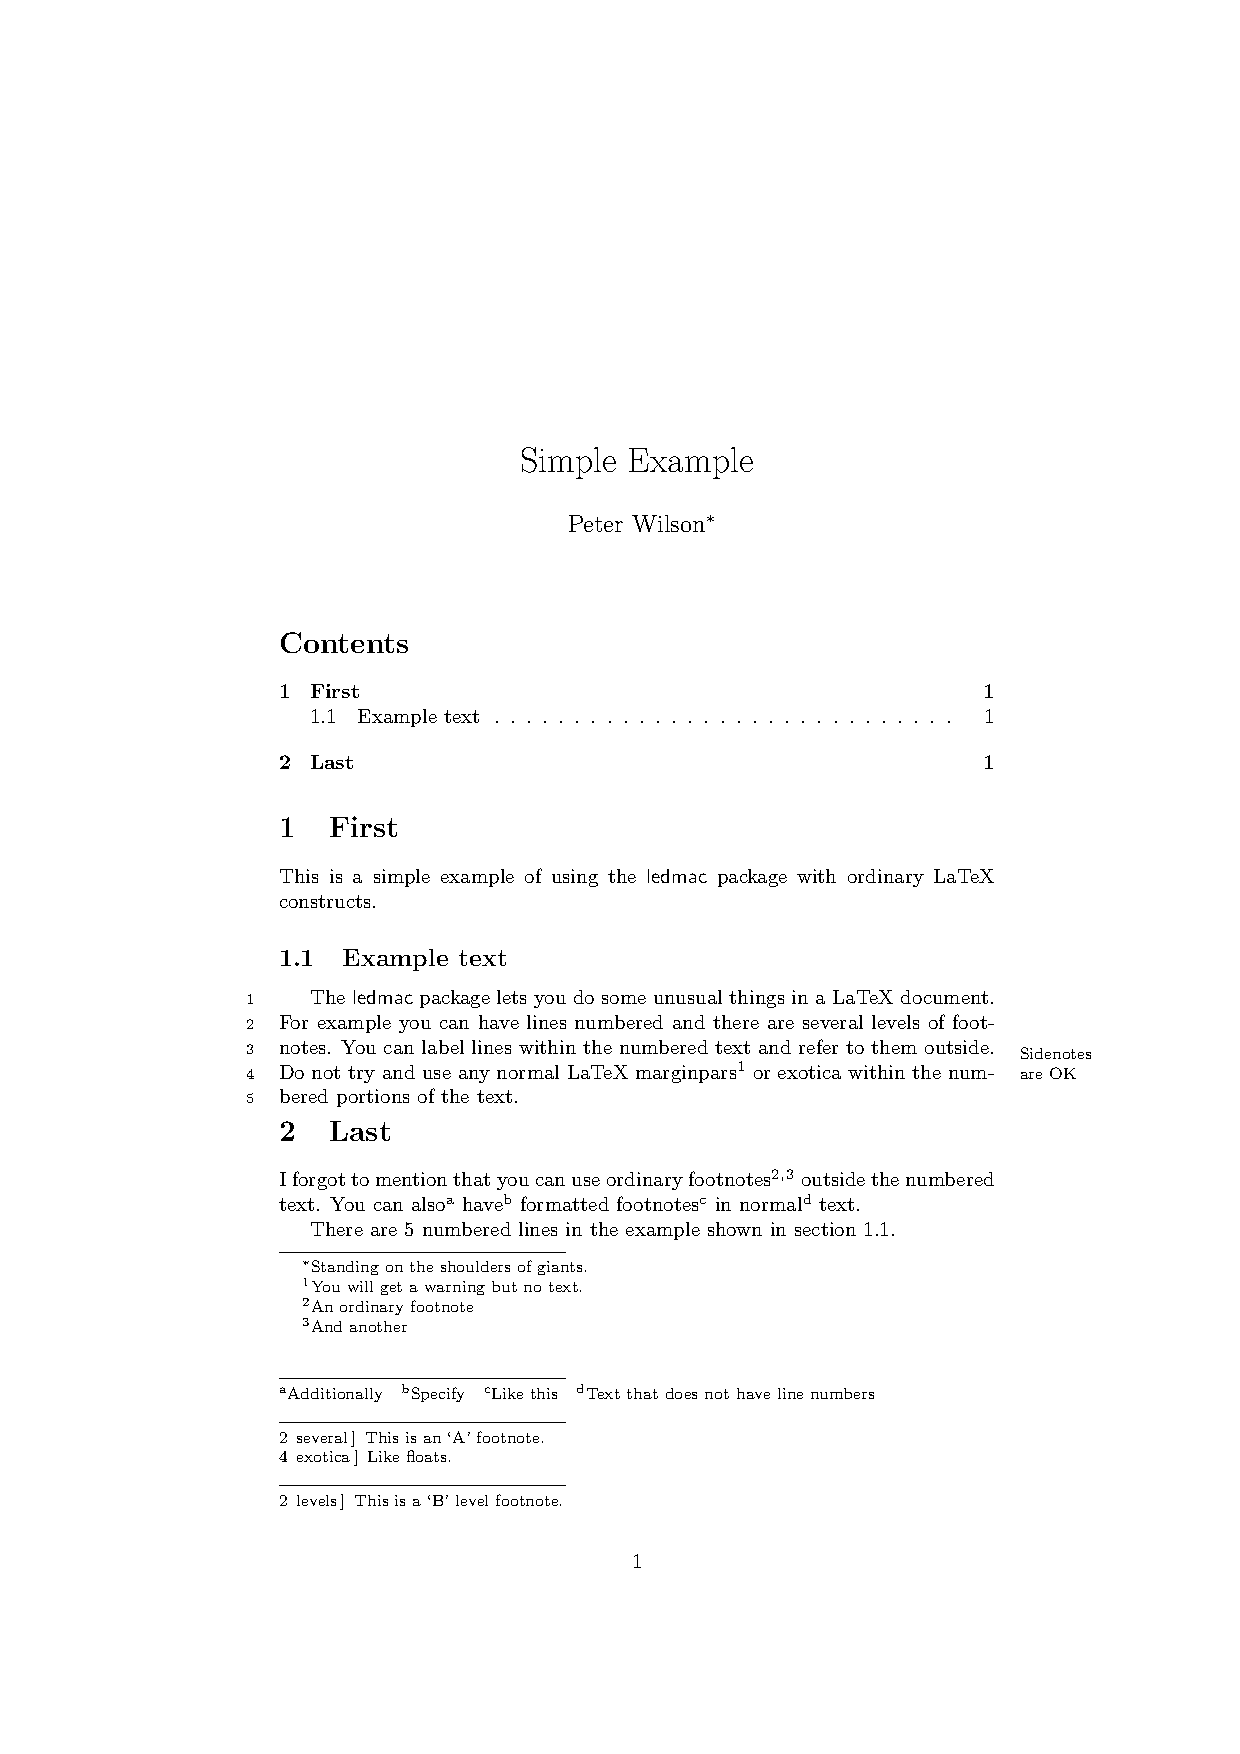
\includegraphics{ledeasy}
% \caption{Output from \file{ledeasy.tex}.}
% \label{easy-out}
% \end{figure}
%
% \begin{figure}[p]
% \centering
% 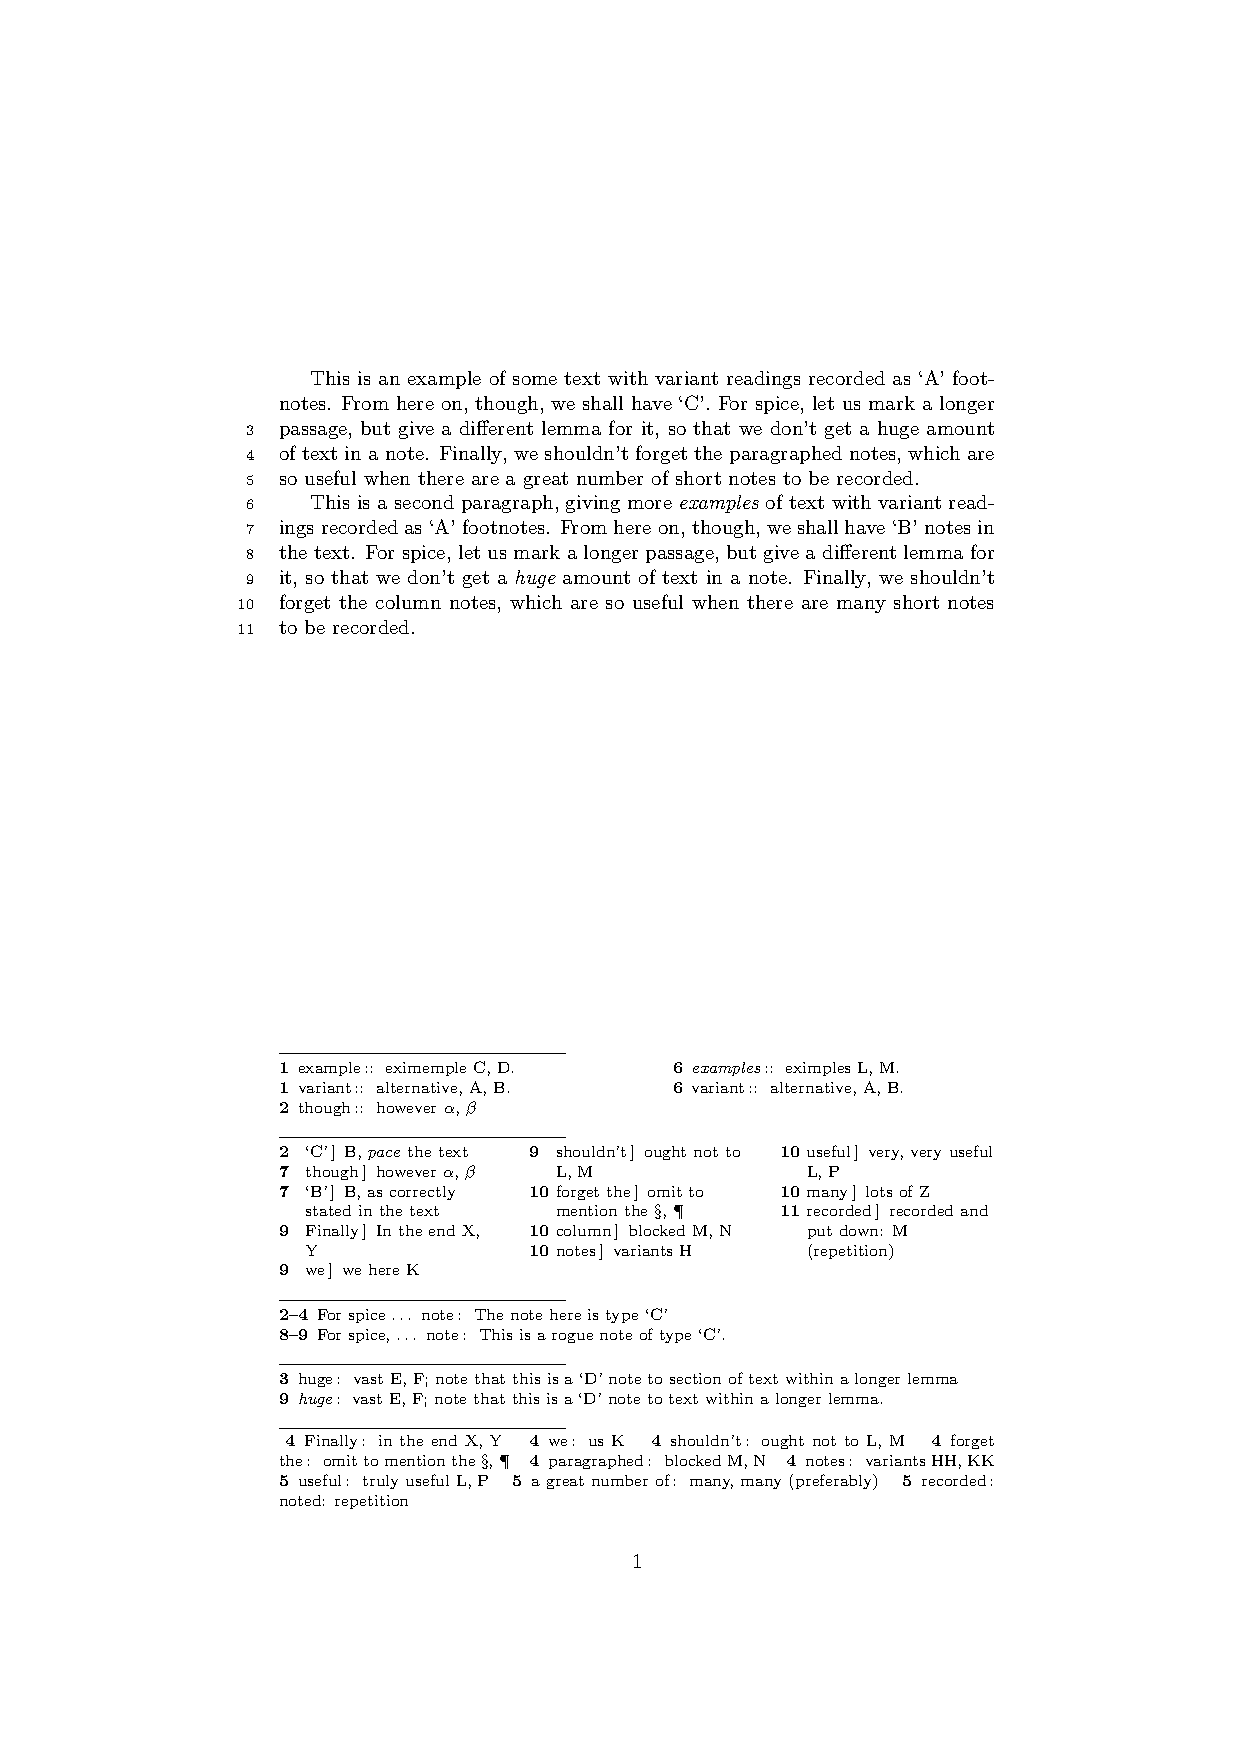
\includegraphics{ledfeat}
% \caption{Output from \file{ledfeat.tex}.}
% \label{features-out}
% \end{figure}
%
% \begin{figure}[p]
% \centering
% 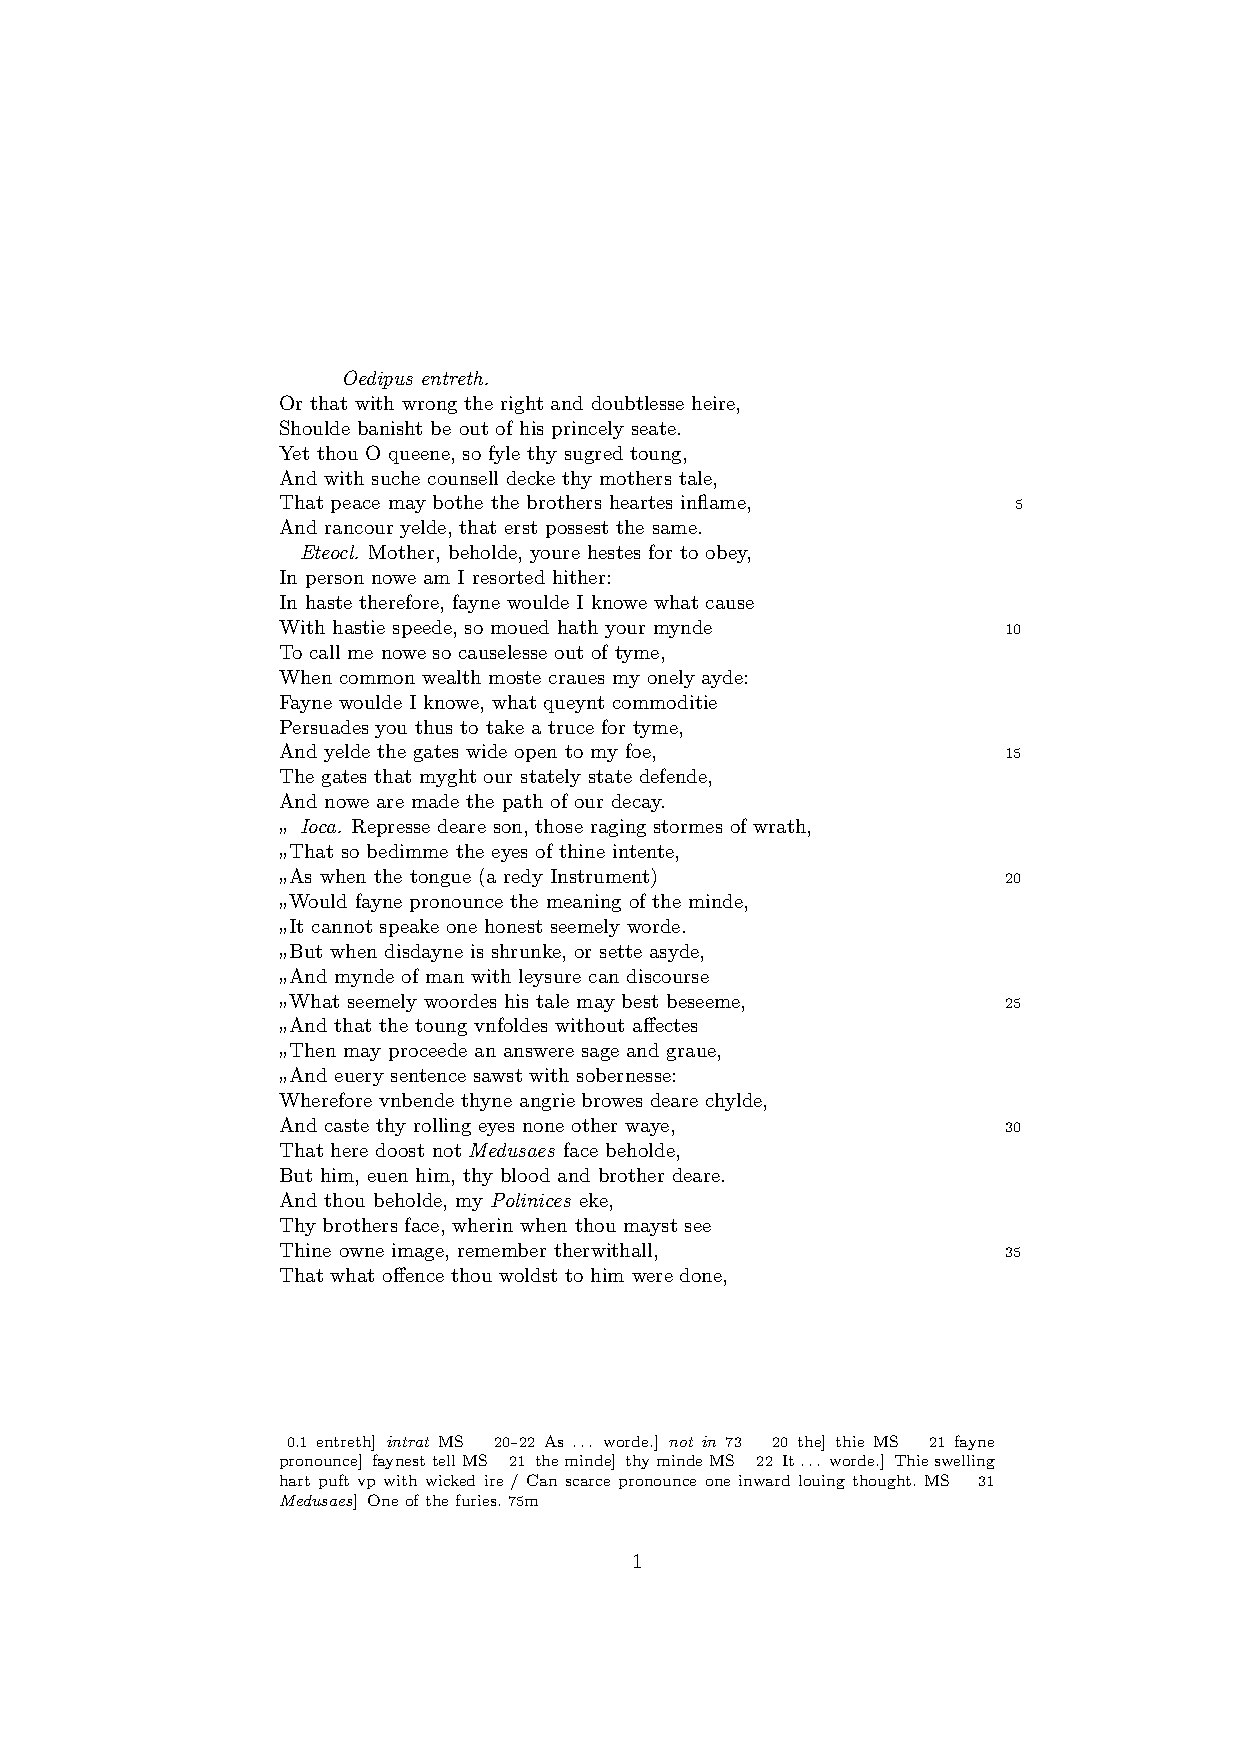
\includegraphics{ledioc}
% \caption{Output from \file{ledioc.tex}.}
% \label{iocasta-out}
% \end{figure}
%
% \begin{figure}[p]
% \centering
% 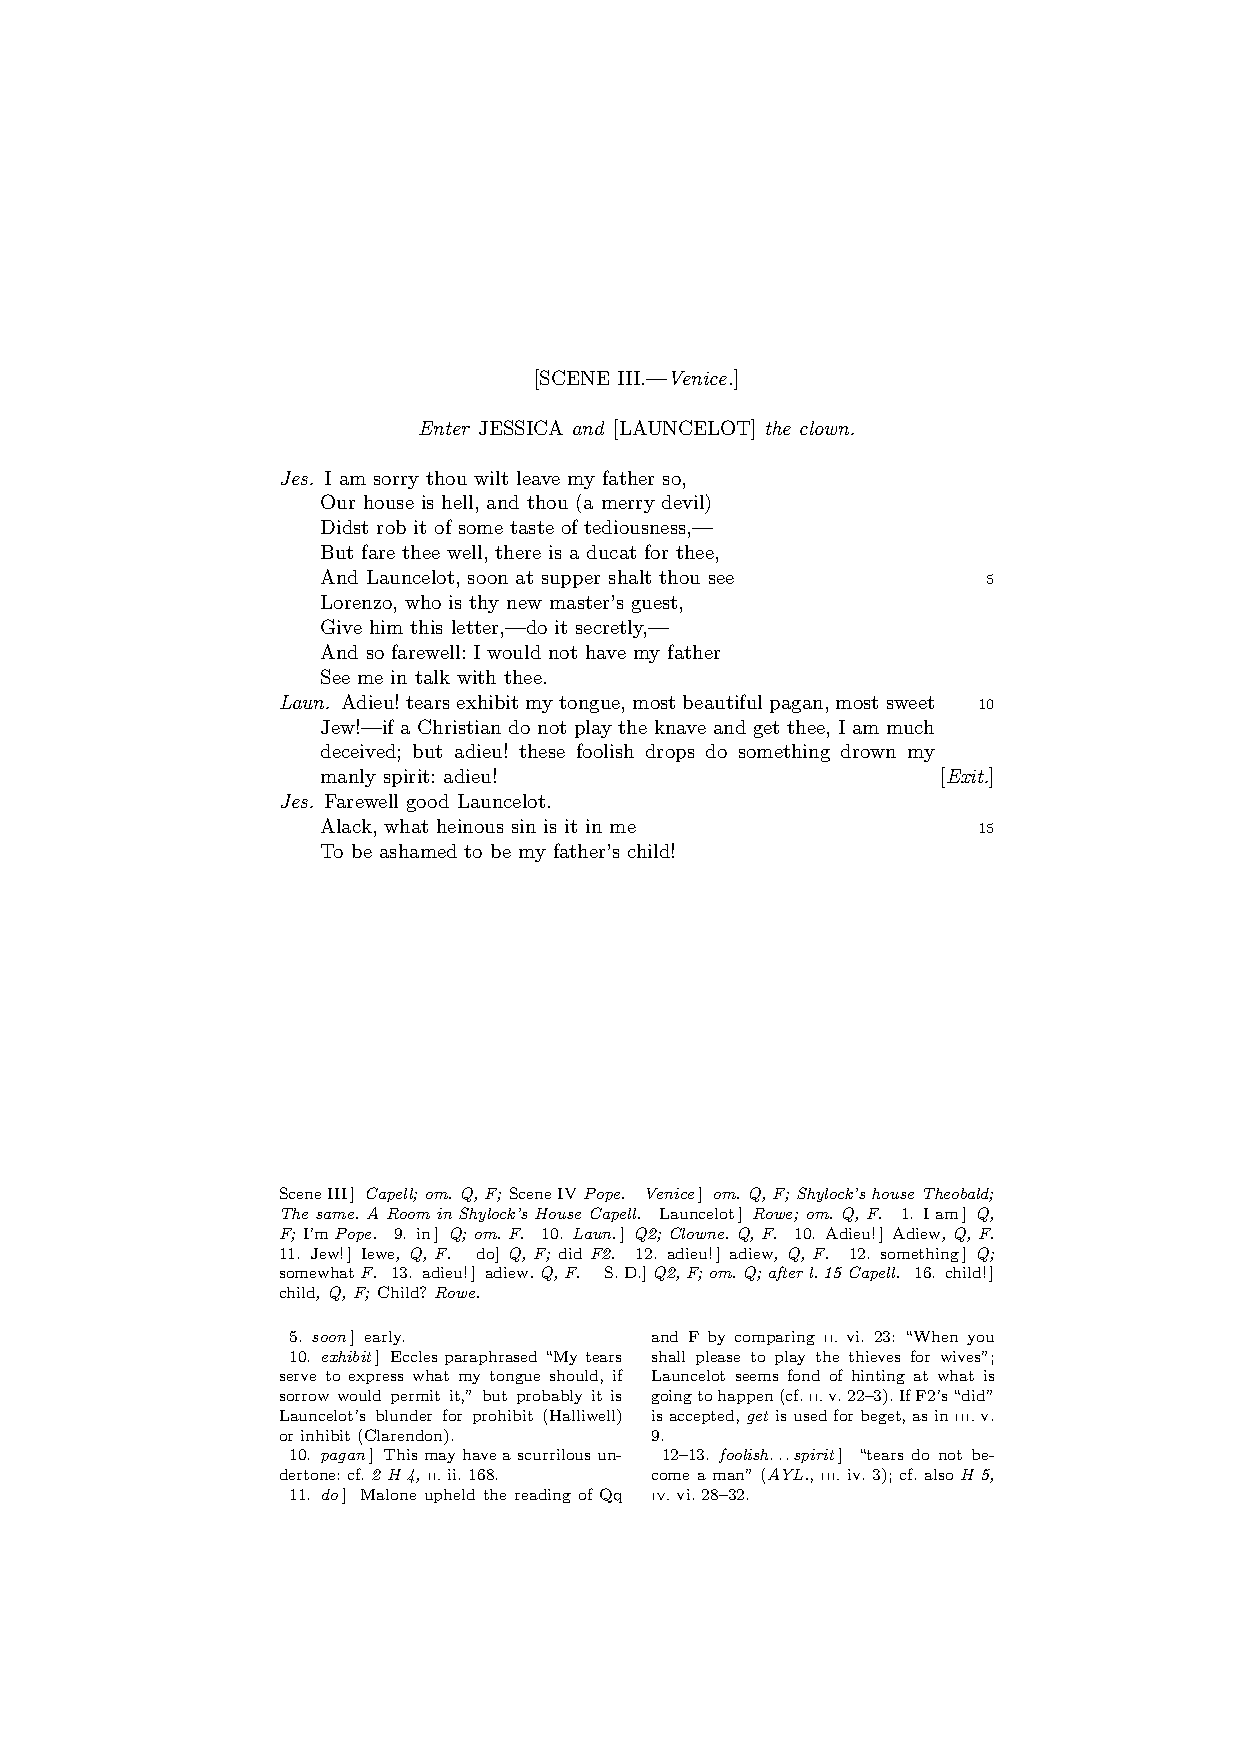
\includegraphics{ledarden}
% \caption{Output from \file{ledarden.tex}.}
% \label{arden-out}
% \end{figure}
%
% \begin{figure}[p]
% \centering
% \hspace*{-2in}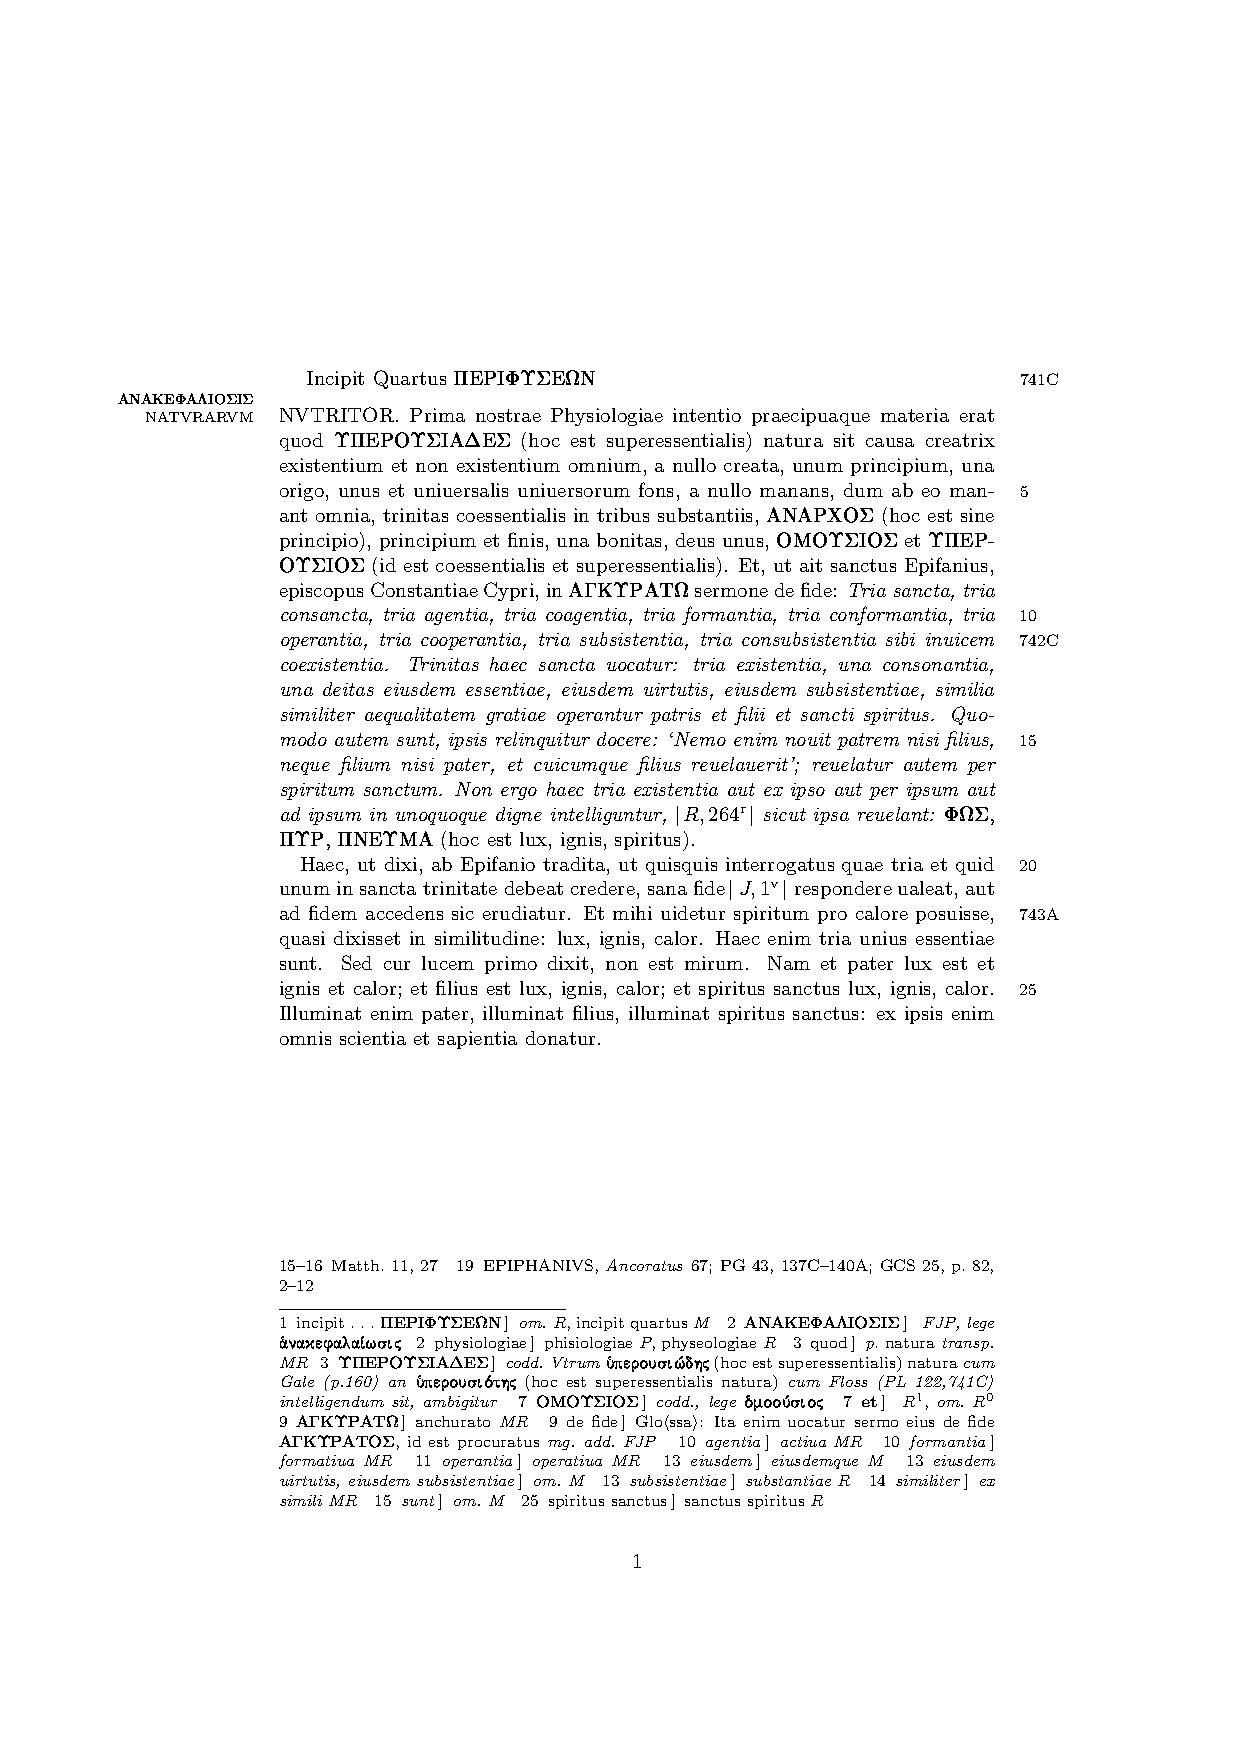
\includegraphics{ledmixed}\hspace*{-2in}
% \caption{Output from \texttt{ledmixed.tex}.}
% \label{periphyseon-out}
% \end{figure}
%
% \begin{figure}[p]
% \centering
% 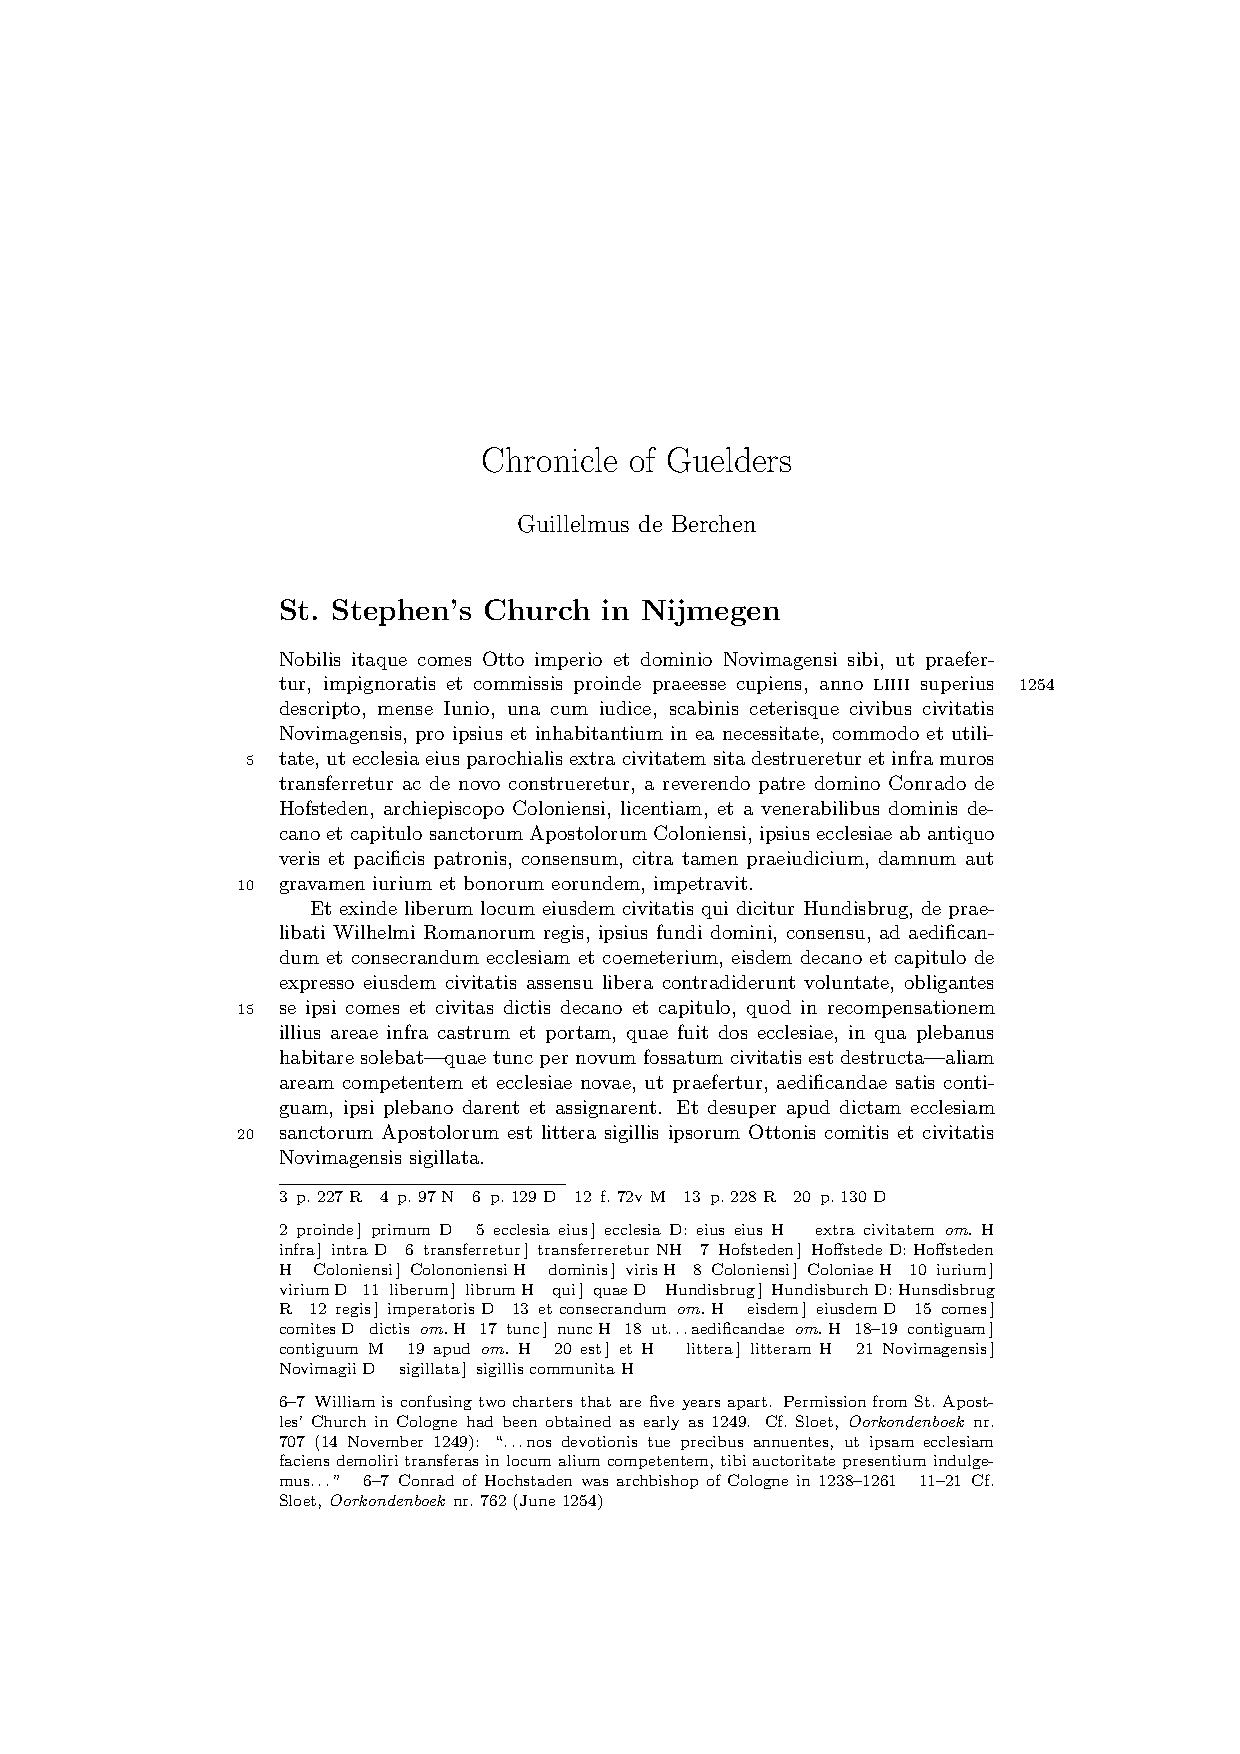
\includegraphics{ledekker}
% \caption{Output from \file{ledekker.tex}.}
% \label{ledekker-out}
% \end{figure}
%
% \begin{figure}[p]
% \centering
% 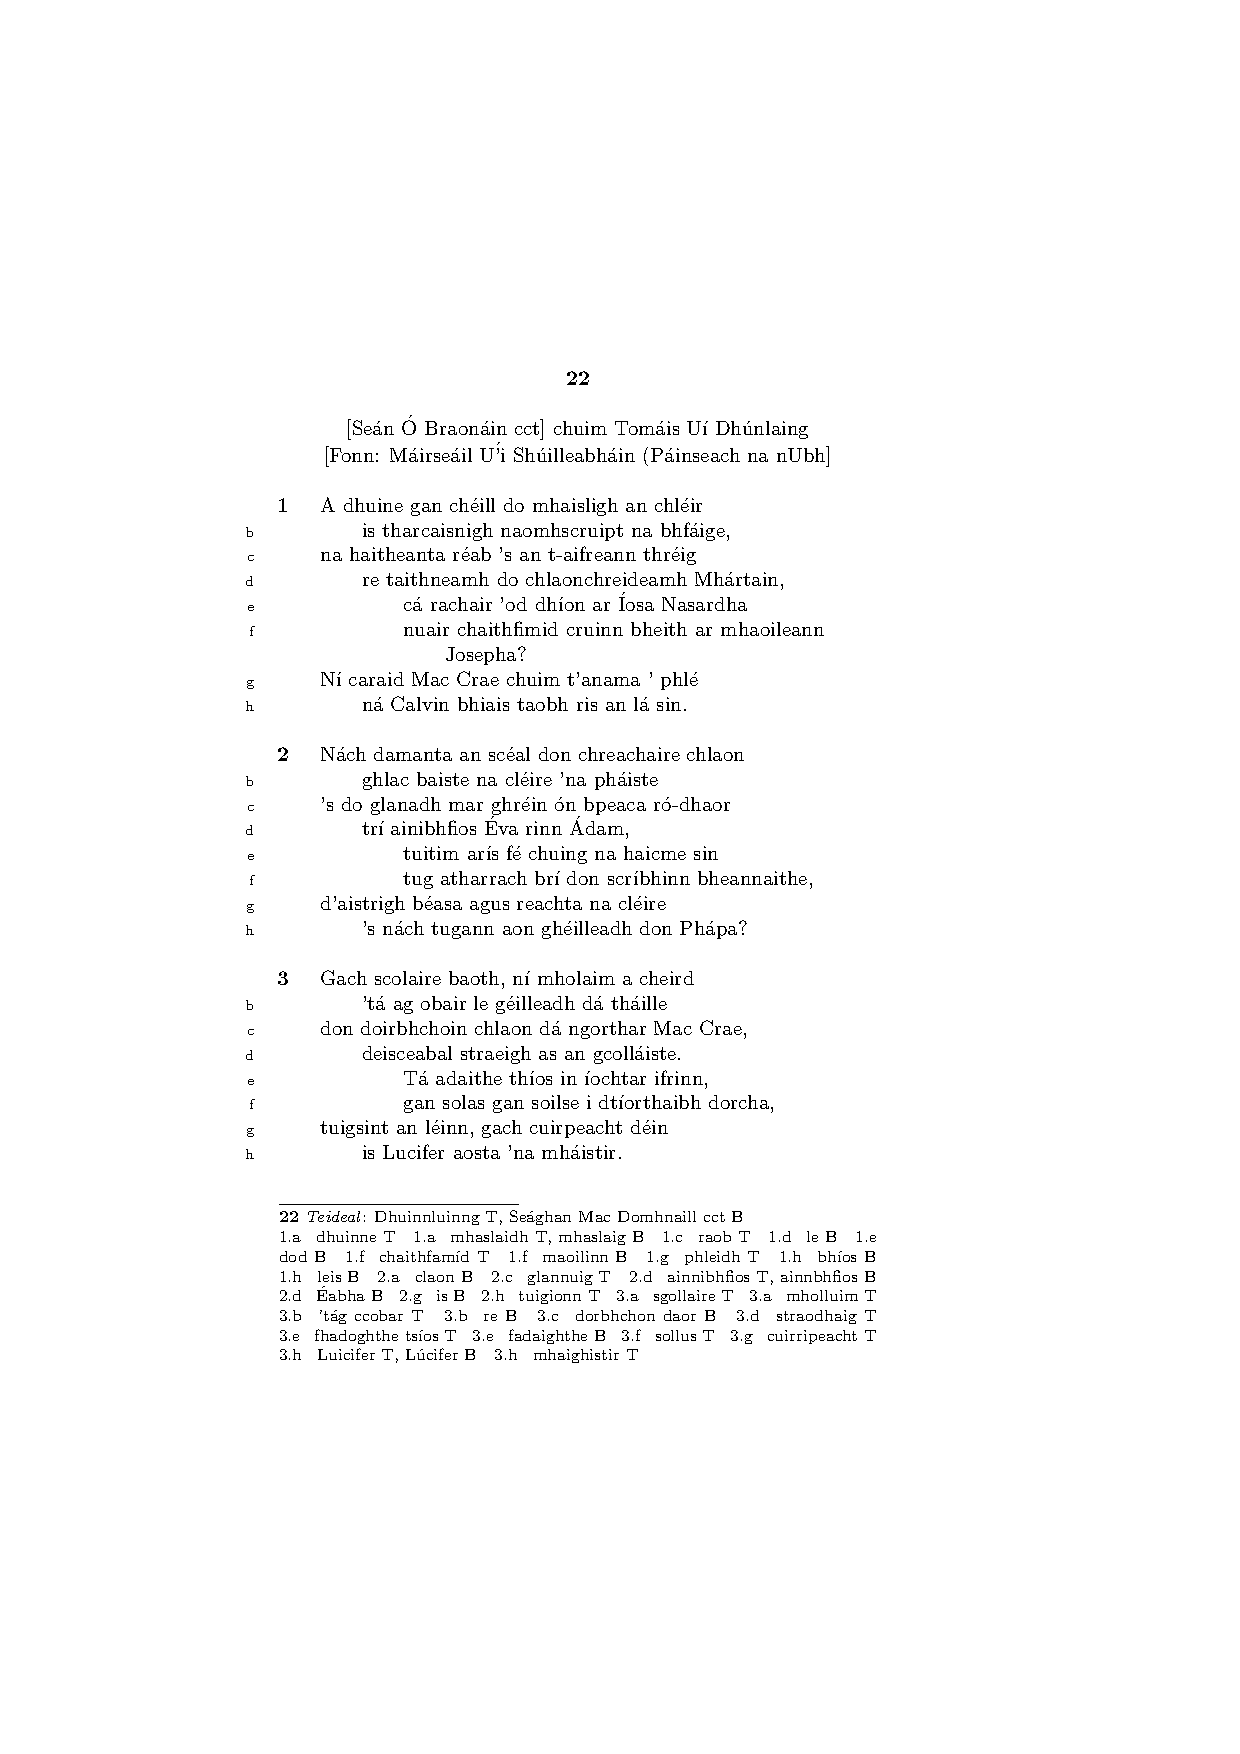
\includegraphics{ledbraonain}
% \caption{Output from \file{ledbraonain.tex}.}
% \label{braonain-out}
% \end{figure}
%
%
% \clearpage
%
% \subsection{Simple example}\label{example:ledeasy}
%
% \begin{PW}
% This made-up example, \file{ledeasy.tex}, is included to show how
% simple it can be to use \edmac{} in a LaTeX document.
% The code is given below and the result is shown in Figure~\ref{easy-out}.
%
% \end{PW}
%
% \medskip
% \hrule
% \medskip
%    \begin{macrocode}
%<*easy>
% ledeasy.tex simple example of the ledmac package
\documentclass{article}
\usepackage{ledmac}
%% number every line
\setcounter{firstlinenum}{1}
\setcounter{linenumincrement}{1}
%% Show some B series familiar footnotes, lettered and paragraphed 
\renewcommand*{\thefootnoteB}{\alph{footnoteB}}
\footparagraphX{B}
%% no endnotes
\noendnotes
%% narrow sidenotes
\setlength{\ledrsnotewidth}{4em}
\title{Simple Example}
\author{Peter Wilson\thanks{Standing on the shoulders of giants.}}
\date{}
\begin{document}
\maketitle
\tableofcontents
\section{First}
   This is a simple example of using the \textsf{ledmac} 
package with ordinary LaTeX constructs.

\subsection{Example text}\label{subsec}

\beginnumbering
\pstart
The \textsf{ledmac} package lets you do some unusual things in
a LaTeX document. For example you can have lines numbered and 
there are  
\edtext{several}{\Afootnote{This is an `A' footnote.}} 
\edtext{levels}{\Bfootnote{This is a `B' level footnote.}}
of footnotes.
You can label lines within the numbered text and refer to them 
outside. Do not try and use any normal LaTeX 
marginpars\footnote{You will get a warning but no text.}%
\ledrightnote{Sidenotes are OK}
or \edtext{exotica}{\Afootnote{Like floats.}}
within the numbered portions of the text\edlabel{line}.
\pend
\endnumbering

\section{Last}

    I forgot to mention that you can use ordinary 
footnotes\footnote{An ordinary footnote}\footnote{And another} 
outside the numbered text. You can also\footnoteB{Additionally}
have\footnoteB{Specify} formatted footnotes\footnoteB{Like this}
in normal\footnoteB{Text that does not have line numbers} text.

   There are \lineref{line} numbered lines in the example shown 
in section~\ref{subsec}.

\end{document}
%</easy>
%    \end{macrocode}
%
%
% \subsection{General example of features} \label{example:ledfeat}
%
% This made-up example, \file{ledfeat.tex}, is included purely to illustrate
% some of \Ledmac's main features.  It is hard to find real-world
% examples that actually use as many layers of notes as this, so we made
% one up.  The example is a bit tricky to read, but close study and
% comparison with the output (Figure~\ref{features-out}) will be
% illuminating.
%
% \begin{PW}
% I have converted the original TeX code to look more like LaTeX code.
% \end{PW}
%
% \medskip
% \hrule
% \medskip
%    \begin{macrocode}
%<*features>
% ledfeat.tex  Small test file for ledmac package
\documentclass{article}
\usepackage{ledmac}

\noendnotes  % we aren't having any endnotes

 \makeatletter
 % I'd like a spaced out colon after the lemma:
 \newcommand{\spacedcolon}{{\rmfamily\thinspace:\thinspace}}
 \renewcommand*{\normalfootfmt}[3]{%
   \ledsetnormalparstuff
   {\notenumfont\printlines#1|}\strut\enspace
   {\select@lemmafont#1|#2}\spacedcolon\enskip#3\strut\par}

 % And I'd like the 3-col notes printed with a hanging indent:
 \renewcommand*{\threecolfootfmt}[3]{%
   \normal@pars
   \hsize .3\hsize
   \setlength{\parindent}{0pt}
   \tolerance=5000       % high, but not infinite
   \raggedright
   \hangindent1.5em \hangafter1
   \leavevmode
   \strut\hbox to 1.5em{\notenumfont\printlines#1|\hfil}\ignorespaces
   {\select@lemmafont#1|#2}\rbracket\enskip
   #3\strut\par\allowbreak}

 % And I'd like the 2-col notes printed with a double colon:
 \newcommand*{\doublecolon}{{\rmfamily\thinspace::\thinspace}}
 \renewcommand*{\twocolfootfmt}[3]{%
   \normal@pars
   \hsize .45\hsize
   \setlength{\parindent}{0pt}
   \tolerance=5000
   \raggedright
   \leavevmode
   \strut{\notenumfont\printlines#1|}\enspace
   {\select@lemmafont#1|#2}\doublecolon\enskip
   #3\strut\par\allowbreak}

 % And in the paragraphed footnotes, I'd like a colon too:
 \renewcommand*{\parafootfmt}[3]{%
   \ledsetnormalparstuff
   {\notenumfont\printlines#1|}\enspace
   {\select@lemmafont#1|#2}\spacedcolon\enskip
   #3\penalty-10 }
 \makeatother

 % I'd like the line numbers picked out in bold.
 \renewcommand{\notenumfont}{\bfseries}
 \lineation{page}
 \linenummargin{inner}
 \setcounter{firstlinenum}{3}       % just because I can
 \setcounter{linenumincrement}{1}
 \foottwocol{A}
 \footthreecol{B}
 \footparagraph{E}
 % I've changed \normalfootfmt, so invoke it again for C and D notes.
 \footnormal{C}
 \footnormal{D}

\begin{document}

 \beginnumbering

 \pstart
 This is an \edtext{example}{
   \Afootnote{eximemple C, D.}}
 of some %\footnote{A normal footnote} 
 text with \edtext{variant}{
   \Afootnote{alternative, A, B.}}
 readings recorded as `A' footnotes.  From here on, \edtext{though}{
   \Afootnote{however $\alpha$, $\beta$}},
 we shall have \edtext{`C'}{
   \Bfootnote{B, \textit{pace} the text}}.
 \edtext{For spice, let us mark a longer passage, but give a different
   lemma for it, so that we don't get a \edtext{huge}{
     \Dfootnote{vast E, F; note that this is
     a `D' note to section of text within a longer lemma}}
   amount of text in a note}{\lemma{For spice \dots\ note}
   \Cfootnote{The note here is type `C'}}.
 \edtext{Finally}{
   \Efootnote{in the end X, Y}},
 \edtext{we}{
   \Efootnote{us K}}
 \edtext{shouldn't}{
   \Efootnote{ought not to L, M}}
 \edtext{forget the}{
   \Efootnote{omit to mention the \S, \P}}
 \edtext{paragraphed}{
   \Efootnote{blocked M, N}}
 \edtext{notes}{
   \Efootnote{variants HH, KK}},
 which are so \edtext{useful}{
   \Efootnote{truly useful L, P}}
 when there are \edtext{a great number of}{
   \Efootnote{many, many (preferably)}}
 short notes to be \edtext{recorded}{
   \Efootnote{noted: repetition}}.
 \pend

 \pstart
 This is a second paragraph, giving more \textit{\edtext{examples}{
   \Afootnote{eximples L, M.}}}
 of text with \edtext{variant}{
   \Afootnote{alternative, A, B.}}
 readings recorded as `A' footnotes.  From here on, \edtext{though}{
   \Bfootnote{however $\alpha$, $\beta$}},
 we  shall have \edtext{`B'}{
   \Bfootnote{B, as correctly stated in the text}} notes in the text.
 \edtext{For spice, let us mark a longer passage, but give a different
   lemma for it, so that we don't get a \textit{\edtext{huge}{
     \Dfootnote{vast E, F; note that this is
     a `D' note to text within a longer lemma.}}}
   amount of text in a note}{\lemma{For spice, \dots\ note}
   \Cfootnote{This is a rogue note of type `C'.}}.
 \edtext{Finally}{
   \Bfootnote{In the end X, Y}},
 \edtext{we}{
   \Bfootnote{we here K}}
 \edtext{shouldn't}{
   \Bfootnote{ought not to L, M}}
 \edtext{forget the}{
   \Bfootnote{omit to mention the \S, \P}}
 \edtext{column}{
   \Bfootnote{blocked M, N}}
 \edtext{notes}{
   \Bfootnote{variants H}},
 which are so \edtext{useful}{
   \Bfootnote{very, very useful L, P}}
 when there are \edtext{many}{
   \Bfootnote{lots of Z}}
 short notes to be \edtext{recorded}{
   \Bfootnote{recorded and put down: M (repetition)}}.
 \pend

 \endnumbering
\end{document}
%</features>
%    \end{macrocode}
% \medskip
% \hrule
% \medskip
%
% \subsection{Gascoigne}
%
% The first real-life example is taken from an edition of George
% Gascoigne's \textit{A Hundreth Sundrie Flowres} that is being
% prepared by G.~W.~Pigman III,\index{Pigman, III$^{rd}$, G. W.} at
% the California Institute of Technology. Figure \ref{iocasta-out}
% shows the result of setting the text with \Ledmac.
%
%
% \begin{PW}
% I have LaTeXified the original code, and removed all the code related
% to the main document layout, relying on the standard LaTeX layout parameters..
% \end{PW}
%
% \medskip
%
% \hrule
% \medskip
%    \begin{macrocode}
%<*ioc>
%% ledioc.tex  
\documentclass{article}
\usepackage{ledmac}

 \noendnotes
 \makeatletter

 \newcommand{\os}{\scriptsize}
 \setcounter{firstsublinenum}{1000}
 \frenchspacing \setlength{\parskip}{0pt} \hyphenpenalty=1000

 % Say \nolinenums if you want no line numbers in the notes.
 \newif\ifnolinenums
 \newcommand{\nolinenums}{\global\nolinenumstrue}
 \newcommand{\linenums}{\global\nolinenumsfalse}

 \renewcommand{\rightlinenum}{\ifbypage@\ifnum\line@num<10\kern.5em\fi\else
 \ifnum\line@num<10\kern1em\else\ifnum\line@num<100
   \kern.5em\fi\fi\fi\kern.5em\numlabfont\the\line@num
   \ifnum\subline@num>0:\the\subline@num\fi}

 \renewcommand{\leftlinenum}{\numlabfont\the\line@num
   \ifnum\subline@num>0:\the\subline@num\fi \kern.5em}
 \linenummargin{outer}
 \lineation{page}

 \newcommand{\ggfootfmt}[3]{%
   \notefontsetup
   \let\par=\endgraf
   \rightskip=0pt \leftskip=0pt
   \setlength{\parindent}{0pt} \parfillskip=0pt plus 1fil
   \ifnolinenums\relax\else
     \begingroup \os \printlines#1|\endgroup
     \enskip
   \fi
   {\rmfamily #2\def\@tempa{#2}\ifx\@tempa\empty
     \else]\enskip\fi#3\penalty-10 }}

 % Now reset the \Afootnote parameters and macros:
 \footparagraph{A}
 \let\Afootfmt=\ggfootfmt
 \dimen\Afootins=\vsize
 \skip\Afootins=3pt plus9pt
 \newcommand*{\ggfootstart}[1]{\vskip\skip\Afootins}
 \let\Afootstart=\ggfootstart

 \newcommand*{\stage}[1]{\pstart\startsub\parindent=0pt
   \hangindent=3em\hangafter=0
   {\itshape #1}\let\par=\finishstage}
 \newcommand{\finishstage}{\pend\endsub}
 \newcommand{\sen}{\leavevmode\lower1ex\hbox{\textrm{''}}}
 \newcommand{\senspeak}[1]{\pstart\obeylines\setbox0=\hbox{\textrm{''}}%
   \leavevmode
   \lower1ex\copy0\kern-\wd0\hskip1em{\textit{#1}}%
   \hbox to1ex{}\ignorespaces}
 \newcommand*{\speak}[1]{\pstart\obeylines\hskip1em{\textit{#1}}%
   \hbox to1ex{}\ignorespaces}
 \def\nospeaker{\parindent=0em\pstart\let\par=\pend}
 \newcommand*{\nospeak}{\pstart\obeylines}
 \makeatother

\begin{document}

 \setlength{\parindent}{0pt}

 \beginnumbering

 \stage{Oedipus \edtext{entreth}{\Afootnote{\textit{intrat} MS}}.}

 \nospeak
 Or that with wrong the right and doubtlesse heire,
 Shoulde banisht be out of his princely seate.
 Yet thou O queene, so fyle thy sugred toung,
 And with suche counsell decke thy mothers tale,
 That peace may bothe the brothers heartes inflame,
 And rancour yelde, that erst possest the same.
 \pend

 \speak{Eteocl.} Mother, beholde, youre hestes for to obey,
 In person nowe am I resorted hither:
 In haste therefore, fayne woulde I knowe what cause
 With hastie speede, so moued hath your mynde
 To call me nowe so causelesse out of tyme,
 When common wealth moste craues my onely ayde:
 Fayne woulde I knowe, what queynt commoditie
 Persuades you thus to take a truce for tyme,
 And yelde the gates wide open to my foe,
 The gates that myght our stately state defende,
 And nowe are made the path of our decay.
 \pend

 \senspeak{Ioca.}Represse deare son, those raging stormes of wrath,
 \sen That so bedimme the eyes of thine intente,
 \edtext{\sen As when \edtext{the}{\Afootnote{thie MS}} tongue %
   (a redy Instrument)
 \sen Would \edtext{fayne pronounce}{\Afootnote{faynest tell MS}} %
   the meaning of \edtext{the minde}{\Afootnote{thy minde MS}},
 \sen \edtext{It}{\lemma{It \dots\ worde.}\Afootnote{Thie %
   swelling hart puft vp with wicked ire / Can scarce pronounce %
   one inward louing thought. MS}} cannot speake one honest %
   seemely worde.}{\lemma{As \dots\ worde.}\Afootnote{\textit{not %
   in} \os73}}
 \sen But when disdayne is shrunke, or sette asyde,
 \sen And mynde of man with leysure can discourse
 \sen What seemely woordes his tale may best beseeme,
 \sen And that the toung vnfoldes without affectes
 \sen Then may proceede an answere sage and graue,
 \sen And euery sentence sawst with sobernesse:
 Wherefore vnbende thyne angrie browes deare chylde,
 And caste thy rolling eyes none other waye,
 That here doost not \edtext{\textit{Medusaes}}{%
 \Afootnote{One of the furies. {\os75}m}} face beholde,
 But him, euen him, thy blood and brother deare.
 And thou beholde, my \textit{Polinices} eke,
 Thy brothers face, wherin when thou mayst see
 Thine owne image, remember therwithall,
 That what offence thou woldst to him were done,
 \pend
 \endnumbering

\end{document}

%</ioc>
%    \end{macrocode}
% \medskip
% \hrule
%
%
% \subsection{Shakespeare} \label{example:ledarden}
%
% The following text illustrates another input file of moderate
% complexity, with two layers of annotation in use. The example is
% taken from the Arden \textit{Merchant of Venice}.\index{Shakespeare, William}
%
%
% \begin{PW}
% I have roughly converted the original TeX file to a LaTeX file.
% The file is below and the result of LaTeXing it is shown in
% Figure~\ref{arden-out}.
% \end{PW}
%
%
% \medskip
% \hrule
% \medskip
%
%    \begin{macrocode}
%<*arden>
%% ledarden.tex
\documentclass{article}
\usepackage{ledmac}

\makeatletter
 \newcommand{\stage}[1]{\rlap{\hbox to \the\linenumsep{%
                        \hfil\llap{[\textit{#1}]}}}}

 \newcommand{\speaker}[1]{\pstart\hangindent2em\hangafter1
   \leavevmode\textit{#1}\enspace\ignorespaces}

 \newcommand{\exit}[1]{\hfill\stage{#1}}

 % LEDMAC customizations:
 \noendnotes
 \setlength{\parindent}{0pt}
 \setlength{\linenumsep}{.4in}
 \rightskip\linenumsep

 \renewcommand{\interparanoteglue}{1em plus.5em minus.1em}

 \newcommand{\scf}{\tiny}
 \let\Afootnoterule=\relax \let\Bfootnoterule=\relax

 \renewcommand{\rightlinenum}{\numlabfont\llap{\the\line@num}}
 \frenchspacing

 % Footnote formats:
 % \nonumparafootfmt is a footnote format without line numbers.
 \newcommand{\nonumparafootfmt}[3]{%
   \ledsetnormalparstuff
   \rightskip=0pt
   \select@lemmafont#1|#2\rbracket\enskip
   \itshape #3\penalty-10 }

 \newcommand{\newparafootfmt}[3]{%
   \ledsetnormalparstuff
   {\notenumfont\printlines#1|}\fullstop\enspace
   {\select@lemmafont#1|#2}\rbracket\enskip
   \itshape #3\penalty-10 }

 \newcommand{\newtwocolfootfmt}[3]{%
   \normal@pars
   \hsize .48\hsize
   \tolerance=5000
   \rightskip=0pt \leftskip=0pt \parindent=5pt
   \strut\notenumfont\printlines#1|\fullstop\enspace
   \itshape #2\/\rbracket\penalty100\hskip .5em plus .5em
   \normalfont #3\strut\goodbreak}

 % Footnote style selections etc. (done last):
 \footparagraph{A}
 \foottwocol{B}
 \let\Afootfmt=\newparafootfmt
 \let\Bfootfmt=\newtwocolfootfmt
 \let\collation=\Afootnote
 \let\note=\Bfootnote
 \lineation{section}
 \linenummargin{right}
 \makeatother

%%%%%%%%%%%%%%%%%%%%%%%%%%%%%%%%

\begin{document}
 \pagestyle{empty}

 % Initially, we don't want line numbers.
 \let\Afootfmt=\nonumparafootfmt

 \beginnumbering
 \pstart
 \centerline{[\edtext{SCENE III}{
   \lemma{Scene III}
   \collation{Capell; om. Q, F; \textnormal{Scene IV} Pope.}}.---%
   \edtext{\textit{Venice}}{
   \collation{om. Q, F; Shylock's house Theobald; The same.
   A Room in Shylock's House Capell.}}.]}
 \pend
 \bigskip

 \pstart
 \centerline{\textit{Enter} JESSICA \textit{and}
   [\edtext{LAUNCELOT}{
   \lemma{Launcelot}
   \collation{Rowe; om. Q, F.}}] \textit{the clown.}} \pend \bigskip

 \let\Afootfmt=\newparafootfmt % we do want line numbers from now

  \setline{0}%

 \speaker{Jes.}\edtext{I am}{
   \collation{Q, F; \textnormal{I'm} Pope.}}
                       sorry thou wilt leave my father so,\\
 Our house is hell, and thou (a merry devil)\\
 Didst rob it of some taste of tediousness,---\\
 But fare thee well, there is a ducat for thee,\\
 And Launcelot, \edtext{soon}{
   \note{early.}}
                        at supper shalt thou see\\
 Lorenzo, who is thy new master's guest,\\
 Give him this letter,---do it secretly,---\\
 And so farewell: I would not have my father\\
 See me \edtext{in}{
   \collation{Q; om. F.}}
              talk with thee.
 \pend

 \speaker{Laun.}
   \edtext{}{\lemma{\textit{Laun.}}\collation{Q2; Clowne. Q, F.}}%
 \edtext{Adieu!}{
   \collation{\textnormal{Adiew}, Q, F.}}
 tears \edtext{exhibit}{
   \note{Eccles paraphrased ``My tears serve to express what my
   tongue should, if sorrow would permit it,'' but probably it is
   Launce\-lot's blunder for prohibit (Halliwell) or inhibit
   (Clarendon).}}
 my tongue, most beautiful \edtext{pagan}{
   \note{This may have a scurrilous undertone: cf. \textit{2 H 4,}
   {\scf II.} \textrm{ii. 168.}}}%
 , most sweet \edtext{Jew!}{
   \collation{\textnormal{Iewe}, Q, F. \quad \textnormal{do]} Q, F;
              \textnormal{did} F2.}}%
 ---if a Christian \edtext{do}{
   \note{Malone upheld the reading of Qq and F by comparing {\scf II.}
    vi. 23: ``When you shall please to play the thieves for
   wives''; Launcelot seems fond of hinting at what is going to
   happen (cf. {\scf II.} v. 22--3). If F2's ``did'' is accepted,
   \textit{get} is used for beget, as in {\scf III.} v. 9.}}
 not play the knave and get thee, I am much deceived; but \edtext{adieu!}{
   \collation{\textnormal{adiew}, Q, F.}}
 these \edtext{foolish drops do \edtext{something}{
   \collation{Q; \textnormal{somewhat} F.}}
 drown my manly spirit}{
   \lemma{foolish\textnormal{\dots}spirit}
   \note{``tears do not become a man'' (\textit{AYL.}, {\scf III.}
   iv. 3); cf. also \textit{H 5,} {\scf IV.} vi. 28--32.}}%
 : \edtext{adieu!}{
   \collation{\textnormal{adiew}. Q, F. \quad \textnormal{S. D.]} Q2, F; om. Q;
   after l. 15 Capell.}}
 \exit{Exit.}
 \pend

 \speaker{Jes.}
 Farewell good Launcelot.\\
 Alack, what heinous sin is it in me\\
 To be ashamed to be my father's \edtext{child!}{
   \collation{\textnormal{child}, Q, F; \textnormal{Child?} Rowe.}}
 \pend
 \endnumbering

\end{document}

%</arden>
%    \end{macrocode}
%
% \medskip
% \hrule
%
%
% \subsection{Classical text edition} \label{example:ledmixed}
%
% The next example, which was extracted from a longer file kindly
% supplied by Wayne Sullivan,\index{Sullivan, Wayne} University
% College, Dublin, Ireland, illustrates the use of \Ledmac{} to
% produce a Latin text edition, the \textit{Periphyseon}, with Greek
% passages.\footnote{The bibliographic details of the forthcoming book
% are: Iohannis Scotti Erivgenae, \textit{Periphyseon} (\textit{De
% Diuisione Naturae}) Liber Qvartvs [Scriptores Latini Hiberniae
% vol.\,xii], (Dublin: School of Celtic Studies, Dublin Institute
% for Advanced Studies, forthcoming 1992).}  The Greek font used is
% that prepared by Silvio Levy\index{Levy, Silvio} and described in 
% \textit{TUGboat}.\footnote{\textit{TUGboat} \textbf{9} (1988), pp.\,20--24.} The
% output of this file is shown in Figure~\ref{periphyseon-out}.
% Note the use of two layers of footnotes to record testimonia and
% manuscript readings respectively.
%
% \begin{PW}
%  I have converted the original \edmac{} example file from TeX
% to something that looks more like LaTeX.
% \end{PW}
%
% ^^A Periphyseon, Liber IV
%
%
% \medskip
% \hrule
% \medskip
%
%    \begin{macrocode}
%<*periph>
% ledmixed.tex
\documentclass{article}
\usepackage{ledmac}

 \noendnotes
%% \overfullrule0 pt
 \lefthyphenmin=3

%    \end{macrocode}
% \begin{PW}
% The LaTeX version uses the \Lpack{lgreek} package to access Silvio Levy's
% greek font. The \texttt{delims} package option 
% subverts\footnote{It actually changes its category code.} the normal meaning
% of \$ to switch in and out of math mode. We have to save the original meaning
% of \$ before calling the package. Later, we use \cs{Ma} and \cs{aM} for math mode
% switching.
% \end{PW}
%    \begin{macrocode}
\let\Ma=$
\let\aM=$
\usepackage[delims]{lgreek}

 % We need an addition to \no@expands since the \active $ in lgreek
 % causes problems:
 \newcommand{\morenoexpands}{\let$=0}

\makeatletter

 \newbox\lp@rbox

 \newcommand{\ffootnote}[1]{%
   \ifnumberedpar@
     \xright@appenditem{\noexpand\vffootnote{f}{{\l@d@nums}{\@tag}{#1}}}%
                                                 \to\inserts@list
     \global\advance\insert@count by 1
 %  \else         %% may be used only in numbered text
 %    \vffootnote{f}{{0|0|0|0|0|0|0}{}{#1}}%
   \fi\ignorespaces}

 \newcommand{\gfootnote}[1]{%
   \ifnumberedpar@
     \xright@appenditem{\noexpand\vgfootnote{g}{#1}}%
                                                 \to\inserts@list
     \global\advance\insert@count by 1
 %  \else         %% may be used only in numbered text
 %    \vgfootnote{g}{#1}%
   \fi\ignorespaces}

 \newcommand{\setlp@rbox}[3]{%
   {\parindent\z@\hsize=2.5cm\raggedleft\scriptsize
   \baselineskip 9pt%
   \global\setbox\lp@rbox=\vbox to\z@{\vss#3}}}

 \newcommand{\vffootnote}[2]{\setlp@rbox#2}

 \newcommand{\vgfootnote}[2]{\def\rd@ta{#2}}
 


 \renewcommand{\affixline@num}{%
   \ifsublines@
     \@l@dtempcntb=\subline@num
     \ifnum\subline@num>\c@firstsublinenum
       \@l@dtempcnta=\subline@num
       \advance\@l@dtempcnta by-\c@firstsublinenum
       \divide\@l@dtempcnta by\c@sublinenumincrement
       \multiply\@l@dtempcnta by\c@sublinenumincrement
       \advance\@l@dtempcnta by\c@firstsublinenum
     \else
       \@l@dtempcnta=\c@firstsublinenum
     \fi
     %
     \ifcase\sub@lock
       \or
         \ifnum\sublock@disp=1
            \@l@dtempcntb=0 \@l@dtempcnta=1
         \fi
       \or
         \ifnum\sublock@disp=2 \else
            \@l@dtempcntb=0 \@l@dtempcnta=1
         \fi
       \or
         \ifnum\sublock@disp=0
            \@l@dtempcntb=0 \@l@dtempcnta=1
         \fi
     \fi
   \else
     \@l@dtempcntb=\line@num
     \ifnum\line@num>\c@firstlinenum
        \@l@dtempcnta=\line@num
        \advance\@l@dtempcnta by-\c@firstlinenum
        \divide\@l@dtempcnta by\c@linenumincrement
        \multiply\@l@dtempcnta by\c@linenumincrement
        \advance\@l@dtempcnta by\c@firstlinenum
     \else
        \@l@dtempcnta=\c@firstlinenum
     \fi
     \ifcase\@lock
        \or
          \ifnum\lock@disp=1
             \@l@dtempcntb=0 \@l@dtempcnta=1
          \fi
        \or
          \ifnum\lock@disp=2 \else
             \@l@dtempcntb=0 \@l@dtempcnta=1
          \fi
        \or
          \ifnum\lock@disp=0
             \@l@dtempcntb=0 \@l@dtempcnta=1
          \fi
     \fi
   \fi
   %
   \ifnum\@l@dtempcnta=\@l@dtempcntb
     \@l@dtempcntb=\line@margin
     \ifnum\@l@dtempcntb>1
       \advance\@l@dtempcntb by\page@num
     \fi
     \ifodd\@l@dtempcntb
 %      #1\rlap{{\rightlinenum}}%
        \xdef\rd@ta{\the\line@num}%
     \else
       \llap{{\leftlinenum}}%#1%
     \fi
   \else
     %#1%
   \fi
   \ifcase\@lock
   \or
     \global\@lock=2
   \or \or
     \global\@lock=0
   \fi
   \ifcase\sub@lock
   \or
     \global\sub@lock=2
   \or \or
     \global\sub@lock=0
   \fi}

 \lineation{page}
 \linenummargin{right}
 \footparagraph{A}
 \footparagraph{B}

\renewcommand{\notenumfont}{\footnotesize}
\newcommand{\notetextfont}{\footnotesize}

 \let\Afootnoterule=\relax
 \count\Afootins=825
 \count\Bfootins=825

 \newcommand{\Aparafootfmt}[3]{%
   \ledsetnormalparstuff
   \scriptsize
   \notenumfont\printlines#1|\enspace
 %      \lemmafont#1|#2\enskip
   \notetextfont
   #3\penalty-10\hskip 1em plus 4em minus.4em\relax}

 \newcommand{\Bparafootfmt}[3]{%
   \ledsetnormalparstuff
   \scriptsize
   \notenumfont\printlines#1|\enspace
   \select@lemmafont#1|#2\rbracket\enskip
   \notetextfont
   #3\penalty-10\hskip 1em plus 4em minus.4em\relax }
 \makeatother

 \let\Afootfmt=\Aparafootfmt
 \let\Bfootfmt=\Bparafootfmt
 \def\lemmafont#1|#2|#3|#4|#5|#6|#7|{\scriptsize}
 \parindent=1em

 \newcommand{\lmarpar}[1]{\edtext{}{\ffootnote{#1}}}
 \newcommand{\rmarpar}[1]{\edtext{}{\gfootnote{#1}}}
 \emergencystretch40pt

%%%%%%%%%%%%%%%%%%%%%%%%%%%%%%%%%%%%%%%%%%%%%%

\begin{document}

 \beginnumbering
 \pstart
 \rmarpar{741C}
 \noindent \edtext{Incipit Quartus $PERIFUSEWN$}{%
 \lemma{incipit\ .~.~.\ $PERIFUSEWN$}\Bfootnote{\textit{om.\ R},
 incipit quartus \textit{M}}}
 \pend
 \medskip

 \pstart
 \noindent \edtext{NVTRITOR}{\lemma{$ANAKEFALIOSIS$}\Bfootnote{\textit{
 FJP, lege} $<anakefala'iwsis$}}.\lmarpar{$ANAKEFALIOSIS$
 NATVRARVM} Prima nostrae
 \edtext{Physiologiae}{\lemma{physiologiae}\Bfootnote{phisiologiae
 \textit{P}, physeologiae \textit{R}}} 
 intentio praecipuaque mat\-e\-ria erat 
 \edtext{quod}{\Bfootnote{\textit{p}.\ natura \textit{transp.\ MR}}}
 \edtext{$UPEROUSIADES$}{\Bfootnote{\textit{codd.\ Vtrum}
 $<uperousi'wdhs$ (hoc est superessentialis) natura \textit{cum Gale
 (p.160) an} $<uperousi'oths$ (hoc est superessentialis natura)
 \textit{cum Floss (PL 122,741C) intelligendum sit, ambigitur}}}
 (hoc est superessentialis) natura sit causa creatrix existentium et
 non existentium omnium, a nullo creata, unum principium, una
 origo, unus et uniuersalis uniuersorum fons, a nullo manans, dum
 ab eo manant omnia, trinitas coessentialis in tribus substantiis,
 $ANARQOS$ (hoc est sine principio), principium et finis, una
 bonitas, deus unus, 
 \edtext{$OMOUSIOS$}{\Bfootnote{\textit{codd., lege} $<omoo'usios$}} 
 \edtext{et}{\lemma{\textbf{et}}\Bfootnote{\textit{
 R}\textsuperscript{1}, \textit{om.\ R}\textsuperscript{0}}}
 $UPEROUSIOS$ (id est coessentialis et superessentialis). Et, ut
 ait sanctus Epifanius, episcopus Constantiae Cypri, in
 \edtext{$AGKURATW$}{\Bfootnote{anchurato \textit{MR}}} 
 sermone 
 \edtext{de fide}{\Bfootnote{Glo\Ma\langle\aM ssa\Ma\rangle\aM: Ita
 enim uocatur sermo eius de fide $AGKURATOS$, id est procuratus
 \textit{mg.\ add.\ FJP}}}:
 \begin{itshape}Tria sancta, tria consancta, tria
 \edtext{agentia}{\Bfootnote{actiua \textit{MR}}}, 
 tria coagentia, tria
 \edtext{formantia}{\Bfootnote{formatiua \textit{MR}}}, 
 tria conformantia, tria 
\edtext{operantia}{\Bfootnote{operatiua \textit{MR}}},
 tria cooperantia, tria subsistentia, tria\rmarpar{742C}
 consubsistentia sibi inuicem coexistentia. Trinitas haec
 sancta uocatur: tria existentia, una consonantia, una deitas
 \edtext{eiusdem}{\Bfootnote{eiusdemque \textit{M}}} 
 essentiae,
 \edtext{eiusdem uirtutis, eiusdem
   \edtext{subsistentiae}{\Bfootnote{substantiae \textit{R}}}}{%
 \Bfootnote{\textit{om.\ M}}}, 
 similia 
\edtext{similiter}{\Bfootnote{ex simili \textit{MR}}} 
 aequalitatem gratiae operantur patris et filii et sancti spiritus. 
 Quomodo autem 
 \edtext{sunt}{\Bfootnote{\textit{om.\ M}}}, 
 ipsis relinquitur docere: 
 \edtext{`Nemo enim nouit patrem nisi filius, neque filium nisi pater, 
    et cuicumque filius reuelauerit'}{\Afootnote{Matth.\ 11, 27}}; 
 reuelatur autem per spiritum sanctum. Non ergo haec tria existentia 
 aut ex ipso aut per ipsum aut ad ipsum in unoquoque digne intelliguntur,
 \Ma\mid\! R, 264^{\rm r}\!\mid\aM\ sicut ipsa reuelant:\end{itshape}
 $FWS, PUR, PNEUMA$ 
 \edtext{(hoc est lux, ignis, spiritus)}{\Afootnote{EPIPHANIVS, 
  \textit{Ancoratus} 67; PG~43, 137C--140A; GCS 25, p.~82, 2--12}}.
 \pend

 \pstart
 Haec, ut dixi, ab Epifanio tradita, ut quisquis interrogatus quae
 tria et quid unum in sancta trinitate debeat credere, sana fide
 \Ma\!\mid J, 1^{\rm v}\!\mid\aM\ respondere ualeat, aut ad
 fidem accedens\rmarpar{743A} sic erudiatur. Et mihi uidetur
 spiritum pro calore posuisse, quasi dixisset in similitudine:
 lux, ignis, calor. Haec enim tria unius essentiae sunt. Sed cur
 lucem primo dixit, non est mirum. Nam et pater lux est et ignis
 et calor; et filius est lux, ignis, calor; et 
 \edtext{spiritus sanctus}{\Bfootnote{sanctus spiritus \textit{R}}} 
 lux, ignis, calor. Illuminat enim pater, illuminat filius, illuminat 
 spiritus sanctus: ex ipsis enim omnis scientia et sapientia donatur.
 \pend
 \endnumbering

\end{document}

%</periph>
%    \end{macrocode}
%
% \medskip
% \hrule
%
% ^^A PW: I have removed the bits of the Arabic and Sanskrit examples.
% ^^A PW: the iffalse ... fi trick doesn't work here because of embedded ifs
%
% \subsection{Nijmegen}\label{example:ledekker}
% \changes{v0.2.2}{2003/11/09}{Added the Dekker example}
% \changes{v0.6}{2004/11/16}{Changed version of the Dekker example}
%
% \begin{PW}
% This example, illustrated in Figure~\ref{ledekker-out},
%  was provided in 2004 by Dirk-Jan Dekker\index{Dekker, Dirk-Jan}
% of the Department of Medieval History at the University of 
% Nijmegen\footnote{On 1st September 2004 the University changed its 
% name to Radboud University.}.
% Unlike earlier examples, this was coded for LaTeX and \Ledmac{} from
% the start. I have reformatted the example to help it fit this document;
% any errors are those that I have inadvertently introduced. Note that
% repeated line numbers are eliminated from the footnotes.
% \end{PW}
%
% \medskip
% \hrule
% \medskip
%    \begin{macrocode}
%<*dekker>
%%% This is ledekker.tex, a sample critical text edition
%%% written in LaTeX2e with the ledmac package.
%%% (c) 2003--2004 by Dr. Dirk-Jan Dekker,
%%% University of Nijmegen (The Netherlands)
%%% (PRW) Modified slightly by PRW to fit the ledmac manual

\documentclass[10pt, letterpaper, oneside]{article}
\usepackage[latin]{babel}
\usepackage{ledmac}

\lineation{section}
\linenummargin{left}
\sidenotemargin{outer}

\renewcommand{\notenumfont}{\footnotesize}
\newcommand{\notetextfont}{\footnotesize}

%\let\Afootnoterule=\relax
\let\Bfootnoterule=\relax
\let\Cfootnoterule=\relax

\addtolength{\skip\Afootins}{1.5mm}
%\addtolength{\skip\Bfootins}{1.5mm}
%\addtolength{\skip\Cfootins}{1.5mm}

\makeatletter

\renewcommand*{\para@vfootnote}[2]{%
  \insert\csname #1footins\endcsname
  \bgroup
    \notefontsetup
    \footsplitskips
    \l@dparsefootspec #2\ledplinenumtrue % new from here
    \ifnum\@nameuse{previous@#1@number}=\l@dparsedstartline\relax
      \ledplinenumfalse
     \fi
     \ifnum\previous@page=\l@dparsedstartpage\relax
     \else \ledplinenumtrue \fi
     \ifnum\l@dparsedstartline=\l@dparsedendline\relax
     \else \ledplinenumtrue \fi
     \expandafter\xdef\csname previous@#1@number\endcsname{\l@dparsedstartline}
     \xdef\previous@page{\l@dparsedstartpage} % to here
     \setbox0=\vbox{\hsize=\maxdimen%
       \let\bidi@RTL@everypar\@empty%
       \noindent\csname #1footfmt\endcsname#2}%
      \setbox0=\hbox{\unvxh0}%
      \dp0=0pt
      \ht0=\csname #1footfudgefactor\endcsname\wd0
      \box0
      \penalty0
  \egroup
}

\newcommand*{\previous@A@number}{-1}
\newcommand*{\previous@B@number}{-1}
\newcommand*{\previous@C@number}{-1}
\newcommand*{\previous@page}{-1}

\newcommand{\abb}[1]{#1%
        \let\rbracket\nobrak\relax}
\newcommand{\nobrak}{\textnormal{}}
\newcommand{\morenoexpands}{%
        \let\abb=0%
}

\newcommand{\Aparafootfmt}[3]{%
  \ledsetnormalparstuff
  \scriptsize
  \notenumfont\printlines#1|\enspace
%  \lemmafont#1|#2\enskip
  \notetextfont
  #3\penalty-10\hskip 1em plus 4em minus.4em\relax}
        
\newcommand{\Bparafootfmt}[3]{%
  \ledsetnormalparstuff
  \scriptsize
  \notenumfont\printlines#1|%
  \ifledplinenum
      \enspace
  \else
      {\hskip 0em plus 0em minus .3em}
  \fi
  \select@lemmafont#1|#2\rbracket\enskip
  \notetextfont
  #3\penalty-10\hskip 1em plus 4em minus.4em\relax }
       
\newcommand{\Cparafootfmt}[3]{%
  \ledsetnormalparstuff
  \notenumfont\printlines#1|\enspace
%  \lemmafont#1|#2\enskip
  \notetextfont
  #3\penalty-10\hskip 1em plus 4em minus.4em\relax}

\makeatother

\footparagraph{A}
\footparagraph{B}
\footparagraph{C}

\let\Afootfmt=\Aparafootfmt
\let\Bfootfmt=\Bparafootfmt
\let\Cfootfmt=\Cparafootfmt

\emergencystretch40pt

\author{Guillelmus de Berchen}
\title{Chronicle of Guelders}
\date{}
\hyphenation{archi-epi-sco-po Huns-dis-brug li-be-ra No-vi-ma-gen-si}
\begin{document}
\maketitle
\thispagestyle{empty}

\section*{St.\ Stephen's Church in Nijmegen}
\beginnumbering
\autopar

\noindent
Nobilis itaque comes Otto imperio et dominio Novimagensi sibi, 
ut praefertur, impignoratis et commissis 
\edtext{proinde}{\Bfootnote{primum D}} praeesse cupiens, anno 
\textsc{liiii}\ledsidenote{1254} superius descripto, mense 
Iu\edtext{}{\Afootnote{p.\ 227~R}}nio, una cum iudice, scabinis 
ceterisque civibus civitatis Novimagensis, pro ipsius et 
inhabitantium in ea necessitate,\edtext{}{\Afootnote{p.\ 97~N}} 
commodo et utilitate, ut 
\edtext{ecclesia eius}{\Bfootnote{ecclesia D: eius eius H}} 
parochialis 
\edtext{\abb{extra civitatem}}{\Bfootnote{\textit{om.}~H}} sita 
destrueretur et \edtext{infra}{\Bfootnote{intra D}} muros 
\edtext{transfer\edtext{}{\Afootnote{p.\ 129~D}}retur}%
{\Bfootnote{transferreretur NH}} 
ac de novo construeretur, \edtext{a reverendo patre domino 
\edtext{Conrado de \edtext{Hofsteden}%
{\Bfootnote{Hoffstede D: Hoffsteden H}}, 
archiepiscopo 
\edtext{Coloniensi}{\Bfootnote{Colononiensi H}}}%
{\Cfootnote{Conrad of Hochstaden was archbishop of Cologne in 
1238--1261}}, licentiam}{\Cfootnote{William is confusing two 
charters that are five years apart. Permission from St.\ Apostles' 
Church in Cologne had been obtained as early as 1249. Cf.\ Sloet, 
\textit{Oorkondenboek} nr.\ 707 (14 November 1249): 
``\ldots{}nos devotionis tue precibus annuentes, ut ipsam 
ecclesiam faciens demoliri transferas in locum alium competentem, 
tibi auctoritate presentium indulgemus\ldots{}''}}, et a 
venerabilibus \edtext{dominis}{\Bfootnote{viris H}} decano et 
capitulo sanctorum Apostolorum 
\edtext{Coloniensi}{\Bfootnote{Coloniae H}}, ipsius ecclesiae ab 
antiquo veris et pacificis patronis, consensum, citra tamen 
praeiudicium, damnum aut gravamen 
\edtext{iurium}{\Bfootnote{virium D}} et bonorum eorundem, 
impetravit. 

\edtext{Et exinde \edtext{liberum}{\Bfootnote{librum H}} locum 
eiusdem civitatis \edtext{qui}{\Bfootnote{quae D}} dicitur 
\edtext{Hundisbrug}{\Bfootnote{Hundisburch D: Hunsdisbrug R}}, 
de praelibati Wilhelmi Romanorum 
\edtext{regis}{\Bfootnote{imperatoris D}}, ipsius fundi 
do\edtext{}{\Afootnote{f.\ 72v~M}}mini, consensu, ad aedificandum 
\edtext{\abb{et consecrandum}}{\Bfootnote{\textit{om.}\ H}} 
ecclesi\edtext{}{\Afootnote{p.\ 228~R}}am et coemeterium, 
\edtext{eisdem}{\Bfootnote{eiusdem D}} decano et capitulo de 
expresso eiusdem civitatis assensu libera contradiderunt voluntate, 
obligantes se ipsi \edtext{comes}{\Bfootnote{comites D}} et civitas 
\edtext{\abb{dictis}}{\Bfootnote{\textit{om.}\ H}} decano et 
capitulo, quod in recompensationem illius areae infra castrum et 
portam, quae fuit dos ecclesiae, in qua plebanus habitare 
solebat---quae \edtext{tunc}{\Bfootnote{nunc H}} per novum fossatum 
civitatis est destructa---aliam aream competentem et ecclesiae 
novae, 
\edtext{ut praefertur, aedificandae}{\lemma{\abb{ut\ldots aedificandae}}%
\Bfootnote{\textit{om.}\ H}} satis 
\edtext{contiguam}{\Bfootnote{contiguum M}}, ipsi plebano darent 
et assignarent. Et desuper 
\edtext{\abb{apud}}{\Bfootnote{\textit{om.}\ H}} dictam ecclesiam 
sanctorum Apostolorum \edtext{est}{\Bfootnote{et H}} 
\edtext{littera}{\Bfootnote{litteram H}} sigillis ipsorum 
Ottonis\edtext{}{\Afootnote{p.\ 130~D}} comitis et civitatis 
\edtext{Novimagensis}{\Bfootnote{Novimagii D}} 
\edtext{sigillata}{\Bfootnote{sigillis communita H}}.}%
{\Cfootnote{Cf.\ Sloet, \textit{Oorkondenboek} nr.\ 762 (June 1254)}}

% (PRW) the full document continues on after this point
%%%%%%%%%%%%%%%%%%%%%%%%%%%
\endnumbering
\end{document}
%%%%%%%%%%%%%%%%%%

%</dekker>
%    \end{macrocode}
%
% \medskip
% \hrule
% \medskip
%
% \subsection{Irish verse}\label{example:ledbraonain}
% \changes{v0.3}{2004/02/14}{Added the Braonain example}
%
% \begin{PW}
% This example, illustrated in Figure~\ref{braonain-out},
% is a somewhat modified and shortened version of Wayne Sullivan's example 
% demonstration for \edstanza.
%
%  The stanza lines are numbered according to the source verse lines,
% not according to the printed lines. For example, the
% sixth (`f') line in the first stanza is printed as two lines as the source
% line was too long to fit on one printed line. Note that if you process
% this yourself you will get error reports about counters the first time 
% through; this is because alphabetic counters, like roman numerals, have no
% notion of zero.
%
%    As is fairly typical of critical edition typesetting, some of
% \Lpack{ledmac}'s internal macros had to be modified to get the
% desired effects.
% \end{PW}
%
% \medskip
% \hrule
% \medskip
%    \begin{macrocode}
%<*braonain>
%%% This is ledbraonain.tex, a sample critical verse edition.
%%% Originally written for TeX processing with edmac and edstanza
%%% by Wayne Sullivan.
%%% Extensively modified by Peter Wilson for LaTeX and the ledmac package.

\documentclass{article}
\usepackage{ledmac}

\setlength{\textheight}{40pc}
\setlength{\textwidth}{24pc}
\bigskipamount=12pt plus 6pt minus 6pt
\newcommand*{\notetextfont}{\footnotesize}

%%%               Just one footnote series
\footparagraph{C}
\count\Cfootins=800
\makeatletter
%%                but using two different formats
\def\xparafootfmt#1#2#3{%
  \ledsetnormalparstuff
  {\notenumfont\printlines#1|}\enspace
%%%  {\select@lemmafont#1|#2}\rbracket\enskip
       \notetextfont #3\penalty-10 }
\def\yparafootfmt#1#2#3{%
  \ledsetnormalparstuff
%%%  {\notenumfont\printlines#1|}\enspace
%%%  {\select@lemmafont#1|#2}\rbracket\enskip
       \notetextfont #3\penalty-10 }

\let\Cfootfmt=\xparafootfmt
\skip\Cfootins=\bigskipamount
\makeatother

%% This is the default, but just to demonstrate...
\setlength{\stanzaindentbase}{20pt}

%%                  MUST SET THE INDENTS
%% indent multiples; first=hangindent.
%% Must all be non-negative whole numbers
\setstanzaindents{4,1,2,1,2,3,3,1,2,1} 

%%                  Set stanza line penalties
%% Must be nonnegative whole numbers.
%% An initial zero indicates no penalties.
\setstanzapenalties{1,5000,10500,5000,10500,5000,5000,5000,0}
%\setstanzapenalties{0}% the default

%%                   Put some space between stanzas
\let\endstanzaextra=\bigbreak % ==> \bigskip \penalty -200

%% (almost) force line break in foot paragraph
\mathchardef\IMM=9999
\def\lbreak{\hfil\penalty-\IMM} 

%%                   Number each stanza in bold
\newcounter{stanzanum}
\setcounter{stanzanum}{0}
\newcommand*{\numberit}{%
  \flagstanza[0.5\stanzaindentbase]{\textbf{\thestanzanum}}}
%% Use the hook to insert the number (and counteract a new line)
%% and reset the line number to zero
\newcommand*{\startstanzahook}{\refstepcounter{stanzanum}%
  \numberit\vskip-\baselineskip%
  \setlinenum{0}}

%% Want to label the footnotes with the stanza and line number
%% We'll use \linenum to replace the sub-line number
%% with the stanza number, redefining \edtext to do this
%% automatically for us.
%%%%%%%%%%%%%%%%%%%%%%%%%
\makeatletter

\renewcommand{\edtext}[2]{\leavevmode
  \begingroup
    \no@expands
    \xdef\@tag{#1}%
    \set@line
    \global\insert@count=0
    \ignorespaces \linenum{||\the\c@stanzanum}#2\relax
    \flag@start
  \endgroup
  #1%
  \ifx\end@lemmas\empty \else
    \gl@p\end@lemmas\to\x@lemma
    \x@lemma
    \global\let\x@lemma=\relax
  \fi
  \flag@end}

%% We need only a very simple macro for footnote numbers,
%% to produce the stanza number (sub-line) then the line number.
\def\printstanzalines#1|#2|#3|#4|#5|#6|#7|{\begingroup
  #3\fullstop \linenumrep{#2}
  \endgroup}
\let\oldprintlines\printlines

\makeatother
%%%%%%%%%%%%%%%%%%%%%%%%%

\pagestyle{empty}

\begin{document}

\beginnumbering

\pstart  \centering \textbf{22}  \pend

\bigskip
%% do not print line number beside heading
\setcounter{firstlinenum}{1000}  
%% and heading footnotes use a different format
\let\Cfootfmt=\yparafootfmt

\pstart
\centerline{[Se\'an \'O Braon\'ain cct] chuim Tom\'ais U\'{\i}
\edtext{Dh\'unlaing}{\Cfootnote{\textbf{22} \textit{Teideal}: Dhuinnluinng T,
Se\'aghan Mac Domhnaill cct B\lbreak}}}
\pend

\pstart
\centerline{[Fonn: M\'airse\'ail U\'{'i} Sh\'uilleabh\'ain (P\'ainseach
             na nUbh]}
\pend

\bigskip

%%           revert to the regular footnote format
\let\Cfootfmt=\xparafootfmt 
%%           but use our special number printing routine
\let\printlines\printstanzalines
%%           Use letters for line numbering
\linenumberstyle{alph}
%%            number lines from the second onwards
\setcounter{firstlinenum}{2}
\setcounter{linenumincrement}{1}

%% Each verse starts with \stanza. 
%% Lines end with &; the last line with \&.

\stanza
A \edtext{dhuine}{\Cfootnote{dhuinne T}} gan ch\'eill do
\edtext{mhaisligh}{\Cfootnote{mhaslaidh T, mhaslaig B}} an chl\'eir&
is tharcaisnigh naomhscruipt na bhf\'aige,&
na haitheanta \edtext{r\'eab}{\Cfootnote{raob T}} 's an 
  t-aifreann thr\'eig&
\edtext{re}{\Cfootnote{le B}} taithneamh do chlaonchreideamh 
  Mh\'artain,&
c\'a rachair \edtext{'od}{\Cfootnote{dod B}} dh\'{\i}on ar 
  \'Iosa Nasardha&
nuair \edtext{chaithfimid}{\Cfootnote{chaithfam\'{\i}d T}} cruinn
bheith ar \edtext{mhaoileann}{\Cfootnote{maoilinn B}} Josepha?&
N\'{\i} caraid Mac Crae chuim t'anama ' 
   \edtext{phl\'e}{\Cfootnote{phleidh T}}&
n\'a Calvin \edtext{bhiais}{\Cfootnote{bh\'{\i}os B}} taobh
\edtext{ris}{\Cfootnote{leis B}} an l\'a sin.\&

\stanza
N\'ach damanta an sc\'eal don chreachaire 
  \edtext{chlaon}{\Cfootnote{claon B}}&
ghlac baiste na cl\'eire 'na ph\'aiste&
's do \edtext{glanadh}{\Cfootnote{glannuig T}} mar ghr\'ein 
  \'on bpeaca r\'o-dhaor&
tr\'{\i} \edtext{ainibhfios}{\Cfootnote{ainnibhfios T, ainnbhfios B}}
\edtext{\'Eva}{\Cfootnote{\'Eabha B}} rinn \'Adam,&
tuitim ar\'{\i}s f\'e chuing na haicme sin&
tug atharrach br\'{\i} don scr\'{\i}bhinn bheannaithe,&
d'aistrigh b\'easa \edtext{agus}{\Cfootnote{is B}} reachta na cl\'eire&
's n\'ach \edtext{tugann}{\Cfootnote{tuigionn T}} aon 
  gh\'eilleadh don Ph\'apa?\&

\stanza
Gach \edtext{scolaire}{\Cfootnote{sgollaire T}} baoth, n\'{\i}
\edtext{mholaim}{\Cfootnote{mholluim T}} a cheird&
\edtext{'t\'a ag obair}{\Cfootnote{'t\'ag ccobar T}} 
  \edtext{le}{\Cfootnote{re B}} g\'eilleadh d\'a th\'aille&
don \edtext{doirbhchoin chlaon}{\Cfootnote{dorbhchon daor B}} 
  d\'a ngorthar Mac Crae,&
deisceabal \edtext{straeigh}{\Cfootnote{straodhaig T}} as an 
  gcoll\'aiste.&
T\'a \edtext{\edtext{adaithe}{\Cfootnote{fadaighthe B}} 
th\'{\i}os}{\Cfootnote{fhadoghthe ts\'{\i}os T}} in 
  \'{\i}ochtar ifrinn,&
gan \edtext{solas}{\Cfootnote{sollus T}} gan soilse i 
  dt\'{\i}orthaibh dorcha,&
tuigsint an l\'einn, gach 
  \edtext{cuirpeacht}{\Cfootnote{cuirripeacht T}} d\'ein&
is \edtext{Lucifer}{\Cfootnote{Luicifer T, L\'ucifer B}} aosta 
  'na \edtext{mh\'aistir}{\Cfootnote{mhaighistir T}}.\&

\endnumbering

\end{document}

%</braonain>
%    \end{macrocode}
%
%
% \medskip
% \hrule
%
%
% \clearpage
%
% \bibliographystyle{alpha}
% \section*{}
% \addcontentsline{toc}{section}{References}
% \begin{thebibliography}{WWW99}
%
% \bibitem[Bre96]{TABMAC}
% Herbert Breger.
% \newblock \tabmac.
% \newblock October 1996.
% \newblock (Available from CTAN in
%            \texttt{macros/plain/contrib/tabmac})
%
% \bibitem[Bur01]{POEMSCOLTUG}
% John Burt.
% \newblock `Typesetting critical editions of poetry'.
% \newblock \emph{TUGboat}, \textbf{22}, 4, pp 353--361, December 2001.
% \newblock (Code available from CTAN in
%            \texttt{macros/latex/contrib/poemscol})
%
% \bibitem[Eck03]{PARALLEL}
% Matthias Eckermann.
% \newblock \emph{The \Lpack{Parallel}-Package}.
% \newblock April 2003.
% \newblock (Available from CTAN in
%            \texttt{macros/latex/contrib/parallel})
%
% \bibitem[Fai03]{FOOTMISC}
% Robin Fairbairns.
% \newblock \emph{\Lpack{footmisc} --- a portmanteau package for 
%            customising footnotes in LaTeX}.
% \newblock February 2003.
% \newblock (Available from CTAN in
%            \texttt{macros/latex/contrib/footmisc})
%
%
% \bibitem[LW90]{EDMACTUG}
% John Lavagnino and Dominik Wujastyk.
% \newblock `An overview of \edmac: a \textsc{Plain} TeX format for
%            critical editions'.
% \newblock \emph{TUGboat}, \textbf{11}, 4, pp. 623--643, November 1990.
% \newblock (Code available from CTAN in
%            \texttt{macros/plain/contrib/edmac})
%
% \bibitem[L\"{u}c03]{EDNOTES}
% Uwe L\"{u}ck.
% \newblock `\textsf{ednotes} --- critical edition typesetting with LaTeX'.
% \newblock \emph{TUGboat}, \textbf{24}, 2, pp. 224--236, 2003.
% \newblock (Code available from CTAN in
%            \texttt{macros/latex/contrib/ednotes})
%
% \bibitem[Sul92]{EDSTANZA}
% Wayne G.~Sullivan.
% \newblock \emph{The file \texttt{edstanza.doc}}.
% \newblock June 1992.
% \newblock (Available from CTAN in
%            \texttt{macros/plain/contrib/edmac})
%
% \bibitem[Wil02]{MEMOIR}
% Peter Wilson.
% \newblock \emph{The \Lpack{memoir} class for configurable typesetting}.
% \newblock November 2002.
% \newblock (Available from CTAN in
%            \texttt{macros/latex/contrib/memoir})
%
% \bibitem[Wil04]{LEDPAR}
% Peter Wilson.
% \newblock \emph{Parallel typesetting for critical editions: 
%                 the \Lpack{ledpar} package}.
% \newblock December 2004.
% \newblock (Available from CTAN in
%            \texttt{macros/latex/contrib/ledmmac})
%
% \bibitem[Wil05]{LEDARAB}
% Peter Wilson.
% \newblock \emph{Critical editions and arabic typesetting:
%                 the \Lpack{ledarab} and \Lpack{afoot} packages}.
% \newblock February 2005.
% \newblock (Available from CTAN in
%            \texttt{macros/latex/contrib/ledmmac})
%
% \end{thebibliography}
%
% \Finale
% \section*{}
% \addcontentsline{toc}{section}{Index}
% \PrintIndex
%
% \section*{}
% \addcontentsline{toc}{section}{Change History}
% \PrintChanges
% \endinput
\endinput

%% \CharacterTable
%%  {Upper-case    \A\B\C\D\E\F\G\H\I\J\K\L\M\N\O\P\Q\R\S\T\U\V\W\X\Y\Z
%%   Lower-case    \a\b\c\d\e\f\g\h\i\j\k\l\m\n\o\p\q\r\s\t\u\v\w\x\y\z
%%   Digits        \0\1\2\3\4\5\6\7\8\9
%%   Exclamation   \!     Double quote  \"     Hash (number) \#
%%   Dollar        \$     Percent       \%     Ampersand     \&
%%   Acute accent  \'     Left paren    \(     Right paren   \)
%%   Asterisk      \*     Plus          \+     Comma         \,
%%   Minus         \-     Point         \.     Solidus       \/
%%   Colon         \:     Semicolon     \;     Less than     \<
%%   Equals        \=     Greater than  \>     Question mark \?
%%   Commercial at \@     Left bracket  \[     Backslash     \\
%%   Right bracket \]     Circumflex    \^     Underscore    \_
%%   Grave accent  \`     Left brace    \{     Vertical bar  \|
%%   Right brace   \}     Tilde         \~}
%%
